
%%
%% forked from https://gits-15.sys.kth.se/giampi/kthlatex kthlatex-0.2rc4 on 2020-02-13
%% expanded upon by Gerald Q. Maguire Jr.
%% This template has been adapted by Anders Sjögren to the University
%% Engineering Program in Computer Science at KTH ICT. This adaptation was to
%% translation of English headings into Swedish as the addition of Swedish.
%% Many thanks to others who have provided constructive input regarding the template.

% Make it possible to conditionally depend on the TeX engine used
\RequirePackage{ifxetex}
\RequirePackage{ifluatex}
\newif\ifxeorlua
\ifxetex\xeorluatrue\fi
\ifluatex\xeorluatrue\fi

\ifxeorlua
% The following is to ensure that the PDF uses a recent version rather than the typical PDF 1-5
%  This same version of PDF should be set as an option for hyperef

\RequirePackage{expl3}
\ExplSyntaxOn
%pdf_version_gset:n{2.0}
%\pdf_version_gset:n{1.5}

%\DocumentMetadata
%{
%% testphase = phase-I, % tagging without paragraph tagging
%% testphase = phase-II % tagging with paragraph tagging and other new stuff.
%pdfversion = 2.0 % pdfversion must be set here.
%}

% Optionally, you can set the uncompress flag to make it easier to examine the PDF
%\pdf_uncompress: % to check the pdf
\ExplSyntaxOff
\else
\RequirePackage{expl3}
\ExplSyntaxOn
%\pdf_version_gset:n{2.0}
\pdf_version_gset:n{1.5}
\ExplSyntaxOff
\fi


%% The template is designed to handle a thesis in English or Swedish
% set the default language to english or swedish by passing an option to the documentclass - this handles the inside tile page
% To optimize for digital output (this changes the color palette add the option: digitaloutput
% To use \ifnomenclature add the option nomenclature
% To use bibtex or biblatex - include one of these as an option
\documentclass[nomenclature, english, bibtex]{kththesis}
%\documentclass[swedish, biblatex]{kththesis}
% if pdflatex \usepackage[utf8]{inputenc}

%% Conventions for todo notes:
% Informational
%% \generalExpl{Comments/directions/... in English}
\newcommand*{\generalExpl}[1]{\todo[inline]{#1}}                

% Language-specific information (currently in English or Swedish)
\newcommand*{\engExpl}[1]{\todo[inline, backgroundcolor=kth-lightgreen40]{#1}} %% \engExpl{English descriptions about formatting}
\newcommand*{\sweExpl}[1]{\todo[inline, backgroundcolor=kth-lightblue40]{#1}}  %% % \sweExpl{Text på svenska}
\newcommand{\inlinecode}[1]{\texttt{#1}}

% warnings
\newcommand*{\warningExpl}[1]{\todo[inline, backgroundcolor=kth-lightred40]{#1}} %% \warningExpl{warnings}

% Uncomment to hide specific comments, to hide **all** ToDos add `final` to
% document class
% \renewcommand\warningExpl[1]{}
% \renewcommand\generalExpl[1]{}
% \renewcommand\engExpl[1]{}
% For example uncommenting the following line hides the Swedish language explanations
% \renewcommand\sweExpl[1]{}


% \usepackage[style=numeric,sorting=none,backend=biber]{biblatex}
\ifbiblatex
    %\usepackage[language=english,bibstyle=authoryear,citestyle=authoryear, maxbibnames=99]{biblatex}
    % alternatively you might use another style, such as IEEE and use citestyle=numeric-comp  to put multiple citations in a single pair of square brackets
    %\usepackage[style=ieee,citestyle=numeric-comp]{biblatex}
    \addbibresource{references.bib}
    %\DeclareLanguageMapping{norsk}{norwegian}
\else
    % The line(s) below are for BibTeX
    \bibliographystyle{bibstyle/myIEEEtran}
    %\bibliographystyle{apalike}
\fi


% include a variety of packages that are useful
%%%%%%%%%%%%%%%%%%%%%%%%%%%%%% Packages %%%%%%%%%%%%%%%%%%%%%%%%%%%%%%
% The following is for use with the KTH cover when not using XeLaTeX or LuaLaTeX
\ifxeorlua\relax
\else
\usepackage[scaled]{helvet}
\fi

%% The following are needed for generating the DiVA page(s)
\usepackage[force-eol=true]{scontents}              %% Needed to save lang, abstract, and keywords
\usepackage{pgffor}                 %% includes the foreach loop

%% Basic packages

%% Links
\usepackage{xurl}                %% Support for breaking URLs

%% Colorize
%\usepackage{color}
\PassOptionsToPackage{dvipsnames, svgnames, table}{xcolor}
\usepackage{xcolor}

\usepackage[normalem]{ulem}
\usepackage{soul}
\usepackage{xspace}
\usepackage{braket}

% to support units and decimal aligned columns in tables
\usepackage[locale=US]{siunitx}

\usepackage{balance}
\usepackage{stmaryrd}
\usepackage{booktabs}
\usepackage{graphicx}	        %% Support for images
\usepackage{multirow}	        %% Support for multirow columns in tables
\usepackage{tabularx}		    %% For simple table stretching
\usepackage{mathtools}
\usepackage{algorithm} 
\usepackage{algorithmic}  
\usepackage{amsmath}
\usepackage[linesnumbered,ruled,vlined,algo2e]{algorithm2e}
% can't use both algpseudocode and algorithmic packages
%\usepackage[noend]{algpseudocode}
%\usepackage{subfig}  %% cannot use both subcaption and subfig packages
\usepackage{subcaption}
\usepackage{optidef}
\usepackage{float}		        %% Support for more flexible floating box positioning
\usepackage{pifont}

%% some additional useful packages
% to enable rotated figures
\usepackage{rotating}	    	%% For text rotating
\usepackage{array}		        %% For table wrapping
\usepackage{mdwlist}            %% various list-related commands
\usepackage{setspace}           %% For fine-grained control over line spacing


\usepackage{enumitem}           %% to allow changes to the margins of descriptions


%% If you are going to include source code (or code snippets) you can use minted in a listings environment
\usepackage{listings}		    %% For source code listing
                                %% For source code highlighting
\usepackage[chapter, cache=false]{minted}   %% If you use minted make sure to use the chapter options to do numbering in the chapter
%\usemintedstyle{borland}

\usepackage{bytefield}          %% For packet drawings


\setlength {\marginparwidth }{2cm} %leave some extra space for todo notes
\usepackage{todonotes}
\usepackage{notoccite} % do not number captions based on their appearance in the TOC


% Footnotes
%\usepackage{perpage}
%\usepackage[perpage]{footmisc} %% use symbols to ``number'' footnotes and reset which symbol is used first on each page
%% Removed option "para" to place each footnote on a separate line. This avoids bad stretching of URLs in footnotes.
\usepackage{footmisc}
\renewcommand{\thefootnote}{\arabic{footnote}}

%% Various useful packages
%%----------------------------------------------------------------------------
%%   pcap2tex stuff
%%----------------------------------------------------------------------------
\usepackage{tikz}
\usepackage{colortbl}
\usetikzlibrary{arrows,decorations.pathmorphing,backgrounds,fit,positioning, decorations.pathreplacing, calc,shapes,calc,trees,positioning,chains,shapes.geometric,matrix,shapes.symbols}

\tikzset{
    >=stealth',
        punktchain/.style={
            rectangle, 
            rounded corners, 
            % fill=black!10,
            draw=black, very thick,
            text width=10em, 
            minimum height=3em, 
            text centered, 
            on chain},
        line/.style={draw, thick, <-},
        element/.style={
            tape,
            top color=white,
            bottom color=blue!50!black!60!,
            minimum width=8em,
            draw=blue!40!black!90, very thick,
            text width=10em, 
            minimum height=3.5em, 
            text centered, 
            on chain},
        every join/.style={->, thick,shorten >=1pt},
        decoration={brace},
        tuborg/.style={decorate},
        tubnode/.style={midway, right=2pt},
}
\usepackage{pgfmath}	% --math engine
\newcommand\bmmax{2}
\usepackage{bm} % bold math


%% Managing titles
% \usepackage[outermarks]{titlesec}
%%%%%%%%%%%%%%%%%%%%%%%%%%%%%%%%%%%%%%%%%%%%%%%%%%%%%%%%%%%%%%%%%%%%%%
%\captionsetup[subfloat]{listofformat=parens}

% to include PDF pages
%\usepackage{pdfpages}

\usepackage{fvextra}
\usepackage{csquotes}               %% Recommended by biblatex
% to provide a float barrier use:
\usepackage{placeins}

\usepackage{comment}  %% Provides a comment environment
\usepackage{refcount}   %% to be able to get an expandable \getpagerefnumber

% for experiments with new cover
\usepackage{eso-pic}
\usepackage[absolute,overlay]{textpos}

% when the package is used, it draws boxes on the page showing the text, footnote, header, and margin regions of the page
%\usepackage{showframe}  
%\usepackage{printlen} % defines the printlength command to print out values of latex variable

\usepackage{xparse}  % to use for commands with optional arguments

\ifnomenclature
\usepackage[nocfg]{nomencl}  %% include refpage, refeq, to have page number and equation number for each nomenclature
\fi

\usepackage{longtable}  % For multipage tables
\usepackage{lscape}     % For landscape pages
\usepackage{needspace}  % to specify needed space, for example to keep listing heading with the listing
\usepackage{metalogo}   % for \XeLaTeX and \LuaLaTeX logos

% to define a command\B to bold font entries in a table
% based on https://tex.stackexchange.com/questions/469559/bold-entries-in-table-with-s-column-type
\usepackage{etoolbox}
\renewcommand{\bfseries}{\fontseries{b}\selectfont}
\robustify\bfseries
\newrobustcmd{\B}{\bfseries}

% To be able to have conditional text #2 that will be included IFF a label is defined, else #3
\newcommand{\iflabelexists}[3]{\ifcsundef{r@#1}{#3}{#2}}


% to allow more than 16 files to be open at once
% Package morewrites Warning: The morewrites package is unnecessary in LuaTeX.
\ifluatex\empty
\else
\usepackage{morewrites}
\fi
\usepackage{geometry}
%\usepackage{glossaries-extra}
\usepackage{svg}
%\usepackage[inkscapeformat=png]{svg}
%\usepackage{adjustbox}
%https://texample.net/tikz/examples/bar-chart/
\usepackage{pgfplots}
%\usepackage{pgf-pie}   
\usepackage{pgfplotstable}
 \pgfplotsset{compat=1.12}

%https://tex.stackexchange.com/questions/554732/bar-plot-does-not-use-defined-color-cycle-list
%\pgfplotscreateplotcyclelist{mycolors}{
%    {blue,fill=blue!30!white,mark=none},
%    {green,fill=green!30!white,mark=none},
%    {brown!60!black,fill=brown!30!white,mark=none},
%    {black,fill=gray,mark=none}
%}
    \tikzset{
        hatch distance/.store in=\hatchdistance,
        hatch distance=10pt,
        hatch thickness/.store in=\hatchthickness,
        hatch thickness=2pt
    }

    \makeatletter
    \pgfdeclarepatternformonly[\hatchdistance,\hatchthickness]{flexible hatch}
    {\pgfqpoint{0pt}{0pt}}
    {\pgfqpoint{\hatchdistance}{\hatchdistance}}
    {\pgfpoint{\hatchdistance-1pt}{\hatchdistance-1pt}}%
    {
        \pgfsetcolor{\tikz@pattern@color}
        \pgfsetlinewidth{\hatchthickness}
        \pgfpathmoveto{\pgfqpoint{0pt}{0pt}}
        \pgfpathlineto{\pgfqpoint{\hatchdistance}{\hatchdistance}}
        \pgfusepath{stroke}
    }
\makeatother
\usetikzlibrary{patterns, patterns.meta}
\usetikzlibrary{decorations.pathreplacing}
\pgfplotscreateplotcyclelist{rustcolors}{
  {red!70!black,mark=none, pattern=
  %{flexible hatch}
  {crosshatch}
  ,pattern color=red!70!white},
  {orange!90!black,mark=none, pattern={vertical lines}, pattern color=orange!90!white},{yellow!50!black,mark=none, pattern={horizontal lines}, pattern color=yellow!90!orange},{green!60!black,mark=none, pattern={north east lines}, pattern color=green!60!black},{brown!80!black,fill=brown!50!white,mark=none},
  {black,fill=gray,mark=none}
}
%\pgfplotscreateplotcyclelist{mycolors}{
%  {black!30!white,fill=black!15!white},
%  {black!50!white,fill=black!35!white},
%  {black!70!white,fill=black!60!white},
%  {black!90!white,fill=black!70!white},
%}
\pgfplotsset{cycle list name=rustcolors}
\pgfplotsset{/pgfplots/bar cycle list/.style={/pgfplots/cycle list name={rustcolors}}}

\usepackage{makecell}

\usepackage[table]{xcolor}

\usepackage{pgf-pie}
%%% Local Variables:
%%% mode: latex
%%% TeX-master: t
%%% End:
% KTH colors for LaTeX documents
%
% Started from kthcolors by:
% Riccardo Sven Risuleo
% 2016-09-06 11:05:40
%
% from https://github.com/KTH-AC/kthcolors
%
% Adapted using the colors from "Graphic Profile Manual KTH" version 180604
% (i.e.. 2018-06-04) 
% see https://intra.kth.se/en/administration/kommunikation/grafiskprofil/kth-s-grafiska-profil-1.844676
% 
% G. Q. Maguire Jr.
% 2021-07-05
%

%\NeedsTexFormat{LaTeX2e}[1994/06/01]
%\ProvidesPackage{kthcolors}[2021/07/85 v3 Latex package with official KTH colors]

\RequirePackage{xcolor}
%% Primary colors
%% As of the new manual, there is only 1 primary color; but with three 
\definecolor{kth-blue}{RGB/cmyk}{25,84,166/0.849,0.494,0,0.349}
\colorlet{kth-blue80}{kth-blue!80!}
\colorlet{kth-blue40}{kth-blue!40!}

% these are no longer used as of 2018-06-04
%\definecolor{kth-red}{RGB/cmyk}{157,16,45/0,0.898,0.713,0.384}
%\definecolor{kth-green}{RGB/cmyk}{98,146,46/0.329,0,0.685,0.427}

%% Secondary colors
\definecolor{kth-lightblue}{RGB/cmyk}{36,160,216/0.833,0.259,0,0.153}
\colorlet{kth-lightblue80}{kth-lightblue!80!}
\colorlet{kth-lightblue40}{kth-lightblue!40!}

%\definecolor{kth-lightred}{RGB/cmyk}{228,54,62/0,0.763,0.728,0.106}
\definecolor{kth-lightred}{RGB}{216,84,151}
\colorlet{kth-lightred80}{kth-lightred!80!}
\colorlet{kth-lightred40}{kth-lightred!40!}

\definecolor{kth-lightgreen}{RGB/cmyk}{176,201,43/0.124,0,0.786,0.212} % olive
\colorlet{kth-lightgreen80}{kth-lightgreen!80!}
\colorlet{kth-lightgreen40}{kth-lightgreen!40!}

% Cool Gray 9C
%\definecolor{kth-coolgray}{RGB}{101,101,108}

% Cool Gray 10 suggested by Martin Krzywinski (see http://mkweb.bcgsc.ca/colorblind) 
\definecolor{kth-coolgray}{RGB}{99,102,106}
\colorlet{kth-coolgray80}{kth-coolgray!80!}
\colorlet{kth-coolgray40}{kth-coolgray!40!}

% Tertiary colors (yet more colors)
% All of these are no longer used
%\definecolor{kth-pink}{RGB/cmyk}{216,84,151/10,0.611,0.301,0.153}
%\definecolor{kth-yellow}{RGB/cmyk}{250,185,25/0,0.26,0.9,0.0196}
%\definecolor{kth-darkgray}{RGB/cmyk}{101,101,108/0.0648,0.0648,0,0.576}
%\definecolor{kth-middlegray}{RGB/cmyk}{189,188,188/0,0.00529,0.00529,0.259}
%\definecolor{kth-lightgray}{RGB/cmyk}{227,229,227/0.00873,0,0.00873,0.102}

%\DeclareOption{gray}{\colorlet{gray}{kth-darkgray}}

% These versions are designed to meet accessability requirements for digital media
% Note that the palette is more limited than for the print version of the colors
\ifdigitaloutput
    % primary color
    \definecolor{kth-blue}{HTML}{1954A6} % Deep sea
    \definecolor{kth-blue80}{HTML}{5E87C0}

    % Secondary colors
    \definecolor{kth-lightblue}{HTML}{2191C4} % Stratosphere
    \definecolor{kth-lightred}{HTML}{D02F80} % Fluorescence
    \definecolor{kth-lightred80}{HTML}{D95599}
    \definecolor{kth-lightgreen}{HTML}{62922E} % Front-lawn
    \definecolor{kth-coolgray}{HTML}{65656C} % Office
    \definecolor{kth-coolgray80}{HTML}{848489}
\fi



%\glsdisablehyper
%\makeglossaries
%\makenoidxglossaries
%%%% Local Variables:
%%% mode: latex
%%% TeX-master: t
%%% End:
% The following command is used with glossaries-extra
\setabbreviationstyle[acronym]{long-short}
% The form of the entries in this file is \newacronym{label}{acronym}{phrase}
%                                      or \newacronym[options]{label}{acronym}{phrase}
% see "User Manual for glossaries.sty" for the  details about the options, one example is shown below
\newacronym{ABI}{ABI}{Application Binary Interface}

\newacronym{API}{API}{Application Programming Interface}
% note the specification of the long form plural in the line below
\newacronym[longplural={Debugging Information Entities}]{DIE}{DIE}{Debugging Information Entity}
%
% The following example also uses options
\newacronym[shortplural={OSes}, firstplural={operating systems (OSes)}]{OS}{OS}{operating system}
%\newacronym{ASLR}{ASLR}{Address Space Layout Randomization}
\newacronym[shortplural={CLA}, firstplural={Cross Language Attacks(s)}]{CLA}{CLA}{Cross Language Attack(s)}
\newabbreviation{CVE}{CVE}{Common Vulnerabilities and Exposures}
\newabbreviation{CWE}{CWE}{Common Weakness Enumeration}
\newacronym{FDA}{FDA}{United States Food and Drug Administration}
\newacronym{FFI}{FFI}{Foreign Function Interface}
% note the use of a non-breaking dash in long text for the following acronym
\newacronym{IQL}{IQL}{Independent Q‑Learning}
\newacronym{IoT}{IoT}{Internet of Things}
\newacronym{JDK}{JDK}{Java development Kit }
\newacronym{JNI}{JNI}{Java Native Interface}
\newacronym{KTH}{KTH}{KTH Royal Institute of Technology}
\newacronym{LAN}{LAN}{Local Area Network}
\newacronym{LOC}{LOC}{lines of code}
\newacronym{NSA}{NSA}{United States of America, National Security Agency}
\newacronym{VM}{VM}{Virtual Machine}
% note the use of a non-breaking dash in the following acronym
\newacronym{WiFi}{Wi‑Fi}{Wireless Fidelity}
\newacronym{WLAN}{WLAN}{Wireless Local Area Network}
%\newacronym{UN}{UN}{United Nations}
%\newacronym{SDG}{SDG}{Sustainable Development Goal}

                %load the acronyms file

\makeatletter
\newcommand{\DeclareLatinAbbrev}[2]{%
  \DeclareRobustCommand{#1}{%
    \@ifnextchar{.}{\textit{#2}}{%
      \@ifnextchar{,}{\textit{#2.}}{%
        \@ifnextchar{!}{\textit{#2.}}{%
          \@ifnextchar{?}{\textit{#2.}}{%
            \@ifnextchar{)}{\textit{#2.}}{%
              {\textit{#2.,\ }}}}}}}}%
}
\newcommand{\DeclareNonLatinAbbrev}[2]{%
  \DeclareRobustCommand{#1}{%
    \@ifnextchar{.}{\textit{#2}}{%
      \@ifnextchar{,}{\textit{#2.}}{%
        \@ifnextchar{!}{\textit{#2.}}{%
          \@ifnextchar{?}{\textit{#2.}}{%
            \@ifnextchar{)}{\textit{#2.}}{%
              {\textit{#2.\ }}}}}}}}%
}
\makeatother
\DeclareLatinAbbrev{\eg}{e.g}
\DeclareLatinAbbrev{\Eg}{E.g}
\DeclareLatinAbbrev{\ie}{i.e}
\DeclareLatinAbbrev{\Ie}{I.e}
\DeclareLatinAbbrev{\etc}{etc}
\DeclareNonLatinAbbrev{\etal}{et~al}

\def\first {$(i)$\xspace}
\def\Second{$(ii)$\xspace}
\def\third {$(iii)$\xspace}
\def\fourth{$(iv)$\xspace}
\def\fifth {$(v)$\xspace}
\def\sixth {$(vi)$\xspace}
\def\seventh{$(vii)$\xspace}
\def\eighth{$(viii)$\xspace}

%%% custom definitions
%% Coloring the links!
\newcommand\myshade{75} % Usage: red!\myshade!black

\definecolor{ForestGreen} {RGB}{34,  139,  34}
\definecolor{HeraldRed2}   {rgb}{0.81, 0.12, 0.15}

\newcommand{\refscolor} {blue}
\newcommand{\linkscolor}{HeraldRed2}
\newcommand{\urlscolor} {ForestGreen}

%% Some definitions of used colors
%\definecolor{darkblue}{rgb}{0.0,0.0,0.3} %% define a color called darkblue
%\definecolor{darkred}{rgb}{0.4,0.0,0.0}
%\definecolor{red}{rgb}{0.7,0.0,0.0}
%\definecolor{lightgrey}{rgb}{0.8,0.8,0.8} 
%\definecolor{grey}{rgb}{0.6,0.6,0.6}
%\definecolor{darkgrey}{rgb}{0.4,0.4,0.4}
%\definecolor{aqua}{rgb}{0.0, 1.0, 1.0}

% For runin headings
\newcommand{\smartparagraph}[1]{\vspace{.05in}\noindent\textbf{#1}}

%% Table of Contents (ToC) depth 
\setcounter{secnumdepth}{4} % how many sectioning levels to assign numbers to
\setcounter{tocdepth}{4}    % how many sectioning levels to show in ToC

%% Limit hyphenation
\hyphenpenalty=9000
\tolerance=5000
% Reduce hyphenation as much as possible:
%\hyphenpenalty=15000
%\tolerance=1000


% For notes by the authors to themselves
\newcommand*{\todoinline}[1]{\textcolor{red}{TODO: #1}}
% https://tex.stackexchange.com/questions/411566/tikz-how-to-modify-pie-chart-with-individually-adjustable-colors-and-point-numb
%\DeclareUnicodeCharacter{2003}{\quad}



\newcommand{\slice}[6]{
  \pgfmathparse{0.5*#1+0.5*#2}
  \let\midangle\pgfmathresult
  % \show\midangle
  % slice
  \draw[thick, pattern=#5, pattern color=#6] (0,0) -- (#1:1) arc (#1:#2:1) -- cycle;

  % outer label
  \node[label=\midangle:#4] at (\midangle:1) {};

  % inner label
  \pgfmathparse{min((#2-#1-10)/110*(-0.3),0)}
  \let\temp\pgfmathresult
  \pgfmathparse{max(\temp,-0.5) + 0.8}
  \let\innerpos\pgfmathresult
  \node at (\midangle:\innerpos) {#3};
}
  % load some additional definitions to make writing more consistent

% The following is needed in conjunction with generating the DiVA data with abstracts and keywords using the scontents package and a modified listings environment
%\usepackage{listings}   %  already included
\ExplSyntaxOn
\newcommand\typestoredx[2]{\expandafter\__scontents_typestored_internal:nn\expandafter{#1} {#2}}
\ExplSyntaxOff
\makeatletter
\let\verbatimsc\@undefined
\let\endverbatimsc\@undefined
\lst@AddToHook{Init}{\hyphenpenalty=50\relax}
\makeatother


\lstnewenvironment{verbatimsc}
    {
    \lstset{%
        basicstyle=\ttfamily\tiny,
        backgroundcolor=\color{white},
        %basicstyle=\tiny,
        %columns=fullflexible,
        columns=[l]fixed,
        language=[LaTeX]TeX,
        %numbers=left,
        %numberstyle=\tiny\color{gray},
        keywordstyle=\color{red},
        breaklines=true,                 % sets automatic line breaking
        breakatwhitespace=true,          % sets if automatic breaks should only happen at whitespace
        %keepspaces=false,
        breakindent=0em,
        %fancyvrb=true,
        frame=none,                     % turn off any box
        postbreak={}                    % turn off any hook arrow for continuation lines
    }
}{}

%% Add some more keywords to bring out the structure more
\lstdefinestyle{[LaTeX]TeX}{
morekeywords={begin, todo, textbf, textit, texttt}
}

%% definition of new command for bytefield package
\newcommand{\colorbitbox}[3]{%
	\rlap{\bitbox{#2}{\color{#1}\rule{\width}{\height}}}%
	\bitbox{#2}{#3}}




% define a left aligned table cell that is ragged right
\newcolumntype{L}[1]{>{\raggedright\let\newline\\\arraybackslash\hspace{0pt}}p{#1}}

% Because backref is not compatible with biblatex
\ifbiblatex
    \usepackage[plainpages=false]{hyperref}
\else
    \usepackage[
    backref=page,
    pagebackref=false,
    plainpages=false,
                            % PDF related options
    unicode=true,           % Unicode encoded PDF strings
    bookmarks=true,         % generate bookmarks in PDF files
    bookmarksopen=false,    % Do not automatically open the bookmarks in the PDF reading program
    pdfpagemode=UseNone,    % None, UseOutlines, UseThumbs, or FullScreen
    destlabel,              % better naming of destinations
    pdfencoding=auto,       % for unicode in 
    ]{hyperref}
    \makeatletter
    \ltx@ifpackageloaded{attachfile2}{
    % cannot use backref if one is using attachfile
    }
    {\usepackage{backref}
    %
    % Customize list of backreferences.
    % From https://tex.stackexchange.com/a/183735/1340
    \renewcommand*{\backref}[1]{}
    \renewcommand*{\backrefalt}[4]{%
    \ifcase #1%
          \or [Page~#2.]%
          \else [Pages~#2.]%
    \fi%
    }
    }
    \makeatother

\fi
\usepackage[all]{hypcap}	%% prevents an issue related to hyperref and caption linking

%% Acronyms
% note that nonumberlist - removes the cross references to the pages where the acronym appears
% note that super  sets the descriptions text aligned
% note that nomain - does not produce a main glossary, thus only acronyms is in the glossary
% note that nopostdot -  prevents there being a period at the end of each entry
\usepackage[acronym, style=super, section=section, nonumberlist, nomain,
nopostdot]{glossaries}
%\newglossarystyle{myglossary}{
%  \setglossarystyle{list} % Use the list style as a base
%  \renewcommand*{\glossaryentryfield}[5]{%
%    \item[\glsentryitem{##1}\glstarget{##1}{##2}] %
%    \hspace{1em} % Add some space between the name and description columns
%   \parbox[t]{\glsdescwidth}{##3} % Set the width of the description column
%    \space ##5 % Add the symbol
%    \glspostdescription % Add any post-description formatting
%    \space ##4 % Add the page number
%    \par
%  }
%}
\setlength{\glsdescwidth}{0.8\textwidth}
\usepackage[]{glossaries-extra}
\ifinswedish
    %\usepackage{glossaries-swedish}
\fi

%% For use with the README_notes
% Define a new type of glossary so that the acronyms defined in the README_notes document can be distinct from those in the thesis template
% the tlg, tld, and dn are the file extensions used for this glossary
\newglossary[tlg]{readme}{tld}{tdn}{README acronyms}

%% For use with the Aïssata's glossary
% Define a new type of glossary distinct from those in the thesis template
% the flg, fld, and fdn are the file extensions used for this glossary
\newglossary[flg]{fullg}{fld}{fdn}{Glossary}
% packages that have to be included after hyperref
\usepackage{doi}
\usepackage{cleveref}           %% Replace Section with a symbol
\usepackage{hyperxmp}           %% to be able to add the copyright information to the PDF metadata

% To be able to attach files to the final PDF
% Note that the package used is attachfile2 and not attachfile - as the former supports most TeX engines
\usepackage{attachfile2}

%% If you are going to set bidirectional text, i.e., left to right and right to left, add bidi as the last package
%\usepackage{bidi}


% For the intro glossary
\newglossary[ilg]{introductiongloss}{ild}{idn}{Introduction Glossary}

%\glsdisablehyper
\makeglossaries
%\makenoidxglossaries

% The following bit of ugliness is because of the problems PDFLaTeX has handling a non-breaking hyphen
% unless it is converted to UTF-8 encoding.
% If you do not use such characters in your acronyms, this could be simplified to just include the acronyms file.
\ifxeorlua
%%% Local Variables:
%%% mode: latex
%%% TeX-master: t
%%% End:
% The following command is used with glossaries-extra
\setabbreviationstyle[acronym]{long-short}
% The form of the entries in this file is \newacronym{label}{acronym}{phrase}
%                                      or \newacronym[options]{label}{acronym}{phrase}
% see "User Manual for glossaries.sty" for the  details about the options, one example is shown below
\newacronym{ABI}{ABI}{Application Binary Interface}

\newacronym{API}{API}{Application Programming Interface}
% note the specification of the long form plural in the line below
\newacronym[longplural={Debugging Information Entities}]{DIE}{DIE}{Debugging Information Entity}
%
% The following example also uses options
\newacronym[shortplural={OSes}, firstplural={operating systems (OSes)}]{OS}{OS}{operating system}
%\newacronym{ASLR}{ASLR}{Address Space Layout Randomization}
\newacronym[shortplural={CLA}, firstplural={Cross Language Attacks(s)}]{CLA}{CLA}{Cross Language Attack(s)}
\newabbreviation{CVE}{CVE}{Common Vulnerabilities and Exposures}
\newabbreviation{CWE}{CWE}{Common Weakness Enumeration}
\newacronym{FDA}{FDA}{United States Food and Drug Administration}
\newacronym{FFI}{FFI}{Foreign Function Interface}
% note the use of a non-breaking dash in long text for the following acronym
\newacronym{IQL}{IQL}{Independent Q‑Learning}
\newacronym{IoT}{IoT}{Internet of Things}
\newacronym{JDK}{JDK}{Java development Kit }
\newacronym{JNI}{JNI}{Java Native Interface}
\newacronym{KTH}{KTH}{KTH Royal Institute of Technology}
\newacronym{LAN}{LAN}{Local Area Network}
\newacronym{LOC}{LOC}{lines of code}
\newacronym{NSA}{NSA}{United States of America, National Security Agency}
\newacronym{VM}{VM}{Virtual Machine}
% note the use of a non-breaking dash in the following acronym
\newacronym{WiFi}{Wi‑Fi}{Wireless Fidelity}
\newacronym{WLAN}{WLAN}{Wireless Local Area Network}
%\newacronym{UN}{UN}{United Nations}
%\newacronym{SDG}{SDG}{Sustainable Development Goal}

    
\else
%%% Local Variables:
%%% mode: latex
%%% TeX-master: t
%%% End:
% The following command is used with glossaries-extra
\setabbreviationstyle[acronym]{long-short}
% The form of the entries in this file is \newacronym{label}{acronym}{phrase}
%                                      or \newacronym[options]{label}{acronym}{phrase}
% see "User Manual for glossaries.sty" for the  details about the options, one example is shown below
% note the specification of the long form plural in the line below
\newacronym[longplural={Debugging Information Entities}]{DIE}{DIE}{Debugging Information Entity}
%
% The following example also uses options
\newacronym[shortplural={OSes}, firstplural={operating systems (OSes)}]{OS}{OS}{operating system}

% note the use of a non-breaking dash in long text for the following acronym
\newacronym{IQL}{IQL}{Independent Q^^e2^^80^^91Learning}

\newacronym{KTH}{KTH}{KTH Royal Institute of Technology}

\newacronym{LAN}{LAN}{Local Area Network}
\newacronym{VM}{VM}{virtual machine}
% note the use of a non-breaking dash in the following acronym
\newacronym{WiFi}{Wi^^e2^^80^^91Fi}{Wireless Fidelity}

\newacronym{WLAN}{WLAN}{Wireless Local Area Network}
\newacronym{UN}{UN}{United Nations}
\newacronym{SDG}{SDG}{Sustainable Development Goal}

\fi

\newglossaryentry{CFI}{
    type=fullg,
    name={control flow integrity (CFI)},
    description={CFI embeds within the software a control-flow policy, that guarantees that the programs follow a path decided ahead of time.}}
    
\newglossaryentry{foreign-function-interface}{
    type=fullg,
    name={foreign function interface (FFI)},
    description={Foreign Function Interface (FFI) is a mechanism in computer programming that enables software written in one programming language to access and use functions or libraries written in another programming language. For systems programming languages such as Rust and Ada, both languages would use the C \gls{ABI}  that defines how data structures are represented in memory.}}
    
\newglossaryentry{memory-corruption}{
    type=fullg,
    name={memory corruption},
    description={Memory corruption happens when memory is altered in a way that was not intended by the programmer. The source of memory corruption is usually programming errors in low-level languages.
\\}}
\newglossaryentry{memory-error}{
    type=fullg,
    name={memory error},
    description={A memory error is common in C/C++ low level languages. It consists of two steps: 1. rendering a pointer unusable, 2. accessing this pointer. A pointer is made obsolete if it goes beyond its bounds or if the object is deallocated. A pointer to a deleted object is known as a dangling pointer. Accessing an out-of-bound pointer is called a spatial error, whereas accessing a dangling pointer is a temporal error.
\\}}
\newglossaryentry{memory-safety}{
    type=fullg,
    name={memory safety},
    description={Memory safety is a programming language property, that controls how memory is used to ensure no bugs related to memory are introduced. Memory safety can be implemented in many different ways, for example, garbage collection, run time detection, or borrow-checker. It ensures memory should not be accessed in an unsafe way. This includes verifying that memory is allocated before usage or that memory is not accessed out-of-bounds.}}
    
\newglossaryentry{ownership}{
    type=fullg,
    name={ownership},
    description={Ownership is a feature of a programming language that guarantees that a place in memory to hold a variable has only one owner. It is inspired by Linear Types (values that must be used exactly once) and Affine types (must be used at most once, \ie it can be ignored). Linear Types enable managing memory of mutable values without a garbage collector\,\cite{ferdowsi_usability_2023}.}}

\newglossaryentry{safety-critical}{
    type=fullg,
    name={safety critical},
    description={The safety-critical industry refers to products such as transportation (aircraft, automobile, railways), as well as medical devices, home appliances, or homes. For safety-critical devices, failure is unacceptable as failures put human life at risk.}}
    
\newglossaryentry{type-safety}{
    type=fullg,
    name={type safety},
    description={Type safety is a feature of the programming language which ensures that variables are of the type they have been declared through the program. Type safety is enforced at compile-time.}}











%ABC
\newglossaryentry{ig:ASLR}
{
    type=introductiongloss,
    name={adress space layout randomization (ASLR)},
    description={Address Space Layout Randomization (ASLR) is a defense technique that mangles the address space of a vulnerable process (libraries, main, heap and stack, as well as memory mapped files) to avoid an attack based on (correct) assumptions on where items lie in memory. Instead, the address space is laid out in a unique manner every time the program is used.}
}


%DEF

\newglossaryentry{ig:DEP}
{
    type=introductiongloss,
    name={data execution prevention (DEP)},
    description={Data Execution Prevention (DEP) is a security feature that makes certain areas in memory non-executable, guaranteeing no malicious code is executed from those areas.
    }
}

\newglossaryentry{ig:EHV}
{
    type=introductiongloss,
    name={exception handler validation},
    description={Exception Handler Validation checks the exception handler (triggered when an exception occurs in the program) against a list of valid handlers before it is executed, to ensure that the pointer is calling a valid address. 
    }
}



%IJK
\newglossaryentry{ig:just-in-time}{
    type=introductiongloss,
    name={just-in-time (JIT)},
    description={A dynamic compilation process that occurs at runtime, which allows to optimization of compiled code for the platform and processor architecture, with the goal to improve performance.
    }
}
\newglossaryentry{ig:ROP}{
    type=introductiongloss,
    name={return-oriented programming (ROP)},
    name={ROP},
    %long={Return Oriented \\ Programming (ROP)},
    description={In ROP, the attacker redirects program execution to a gadget already present in the program memory.
    }
}

\newglossaryentry{ig:stack-cookie}
{
    type=introductiongloss,
    name={stack cookie},
    description={A stack cookie, also known as a stack canary is a security mechanism used to detect stack buffer overflow attacks. It involves placing a random value between the local variables and the function return address on the stack. The canary value is checked when the function returns to ensure that it has not been modified by an attacker. If the canary value has been altered, then it is assumed that a buffer overflow attack has occurred. 
    }
}

%UVWXYZ


















  

% insert the configuration information with author(s), examiner, supervisor(s), ...
%% Information for inside title page


\authorsLastname{Maiga}
\authorsFirstname{Aïssata}
\email{<maiga@kth.se>}
\kthid{u1eg1x6a}
% As per email from KTH Biblioteket on 2021-06-28 students cannot have an OrCiD reported for their degree project
\authorsSchool{\schoolAcronym{EECS}}
%If the student is not in Stockholm, Sweden, add that information here
% This information will be used when generating the acknowledgements signature.
%\authorCity{A City}
%\authorCountry{A Country}
% pass into \authorCityCountryDate{} the month and year for the acknowledgment
% If there is a second author and place, the month, and year are the same, the specify the month and year for the first author:
\authorCityCountryDate{\MONTH\enspace\the\year}
% if there is a second author and the place is different, then say:
%\authorCityCountryDate{}

% If there is a second author - add them here:
%\secondAuthorsLastname{Student}
%\secondAuthorsFirstname{Fake B.}
%\secondemail{b@kth.se}
%\secondkthid{u100002}
% As per email from KTH Biblioteket on 2021-06-28 students cannot have an OrCiD reported for their degree project
\secondAuthorsSchool{\schoolAcronym{ABE}}
%If the student is not in Stockholm, Sweden, add that information here
% This information will be used when generating the acknowledgements signature.
%\secondAuthorCity{A City}
%\secondAuthorCountry{A Country}
% pass into \secondAuthorCityCountryDate{} the month and year for the acknowledgement
%\secondAuthorCityCountryDate{\MONTH\enspace\the\year}
%\secondAuthorCityCountryDate{}

\supervisorAsLastname{Artho}
\supervisorAsFirstname{Cyrille}
\supervisorAsEmail{artho@kth.se}
% If the supervisor is from within KTH add their KTHID, School and Department info
\supervisorAsKTHID{u1tesytk}
\supervisorAsSchool{\schoolAcronym{EECS}}
\supervisorAsDepartment{Computer Science}
% other for a supervisor outside of KTH add their organization info
%\supervisorAsOrganization{Timbuktu University, Department of Pseudoscience}

%If there is a second supervisor add them here:
\supervisorBsLastname{Gilcher}
\supervisorBsFirstname{Florian}
\supervisorBsEmail{florian.gilcher@ferrous-systems.com}
% If the supervisor is from within KTH add their KTHID, School and Department info
%\supervisorBsKTHID{u100003}
%\supervisorBsSchool{\schoolAcronym{ABE}}
%\supervisorBsDepartment{Architecture}
% other for a supervisor outside of KTH add their organization info
\supervisorBsOrganization{Ferrous Systems}

%If there is a third supervisor add them here:
\supervisorCsLastname{Moy}
\supervisorCsFirstname{Yannick}
\supervisorCsEmail{moy@adacore.com}
% If the supervisor is from within KTH add their KTHID, School and Department info
%\supervisorCsKTHID{u100004}
%\supervisorCsSchool{\schoolAcronym{ABE}}
%\supervisorCsDepartment{Public Buildings}
% other for a supervisor outside of KTH add their organization info
\supervisorCsOrganization{AdaCore}

\examinersLastname{Troubitsyna}
\examinersFirstname{Elena}
\examinersEmail{elenatro@kth.se}
% If the examiner is from within KTH add their KTHID, School and Department info
%\examinersKTHID{u1d13i2c}
\examinersSchool{\schoolAcronym{EECS}}
\examinersDepartment{Computer Science}
% other for a examiner outside of KTH add their organization info
%\examinersOrganization{Timbuktu University, Department of Pseudoscience}


\hostcompany{Ferrous Systems} % Remove this line if the project was not done at a host company
%\hostorganization{CERN}   % if there was a host organization


\date{\today}

\courseCycle{2}
\courseCode{DA231X}
\courseCredits{30.0}
\edprogram{Master's Programme, Computer Science, 120 credits}
\programcode{TCSCM}
\degreeName{Degree of Master (120 credits)}
\subjectArea{Computer Science and Engineering}

%\degreeName{Bachelors degree}
% Note that the subject area for a Bachelor's thesis (Kandidatexamen) should be either Technology or Architecture
% If the thesis is in Swedish, these would be: teknik | arkitektur   -- Note the use of lower case
%\subjectArea{Technology}
% if there is a second degree
%\secondProgramcode{CINTE}
%\secondDegreeName{test second degree}
%\secondSubjectArea{test second subject area}

% Note that in the case of both Both Degree of Master of Science in Engineering and Master's degree
% there are two cases: "Both" is used when the field of technology (\subjectArea{}) and the main subject (\secondSubjectArea{} are different and the case "Same" when they are the same.
%% Both case
%\courseCycle{2}
%\courseCode{xxxxxx}
%\courseCredits{30.0}
%\degreeName{Both Degree of Master of Science in Engineering and Master's degree}
%\subjectArea{Biotechnology}
%\secondSubjectArea{Medical Engineering}

%\courseCycle{2}
%\courseCode{xxxxxx}
%\courseCredits{30.0}
%\degreeName{Både civilingenjörsexamen och masterexamen}
%\subjectArea{bioteknik}
%\secondSubjectArea{medicinsk teknik}

%% Same case
%\courseCycle{2}
%\courseCode{xxxxxx}
%\courseCredits{30.0}
%\degreeName{Both Degree of Master of Science in Engineering and Master's degree}
%\subjectArea{Biotechnology}
%\secondSubjectArea{Biotechnology}

%\courseCycle{2}
%\courseCode{xxxxxx}
%\courseCredits{30.0}
%\degreeName{Både civilingenjörsexamen och masterexamen}
%\subjectArea{bioteknik}
%\secondSubjectArea{bioteknik}

% For a CDATE student the following are likely values:
%\programcode{CDATE}
%\courseCycle{2}
%\courseCode{DA231X}
%\courseCredits{30.0}
%\degreeName{Degree of Master of Science in Engineering}
%\subjectArea{Computer Science and Engineering}

% For a TCSCM student the following are likely values:
%\programcode{TCSCM}
%\courseCycle{2}
%\courseCode{DA231X}
%\courseCredits{30.0}
%\degreeName{Master's Programme, Computer Science, 120 credits}
%\subjectArea{Computer Science}

% For a CMETE student the following are likely values:
%\programcode{CMETE}
%\courseCycle{2}
%\courseCode{DA231X}
%\courseCredits{30.0}
%\degreeName{Degree of Master of Science in Engineering}
%\subjectArea{Media Technology}

% For a CINTE student the following are likely values:
%\programcode{CINTE}
%\courseCycle{2}
%\courseCode{DA231X}
%\courseCredits{30.0}
%\degreeName{Degree of Master of Science in Engineering}
%\subjectArea{Information and Communication Technology}


%%%%% for DiVA's National Subject Category information
%%% Enter one or more 3 or 5 digit codes
%%% See https://www.scb.se/contentassets/3a12f556522d4bdc887c4838a37c7ec7/standard-for-svensk-indelning--av-forskningsamnen-2011-uppdaterad-aug-2016.pdf
%%% See https://www.scb.se/contentassets/10054f2ef27c437884e8cde0d38b9cc4/oversattningsnyckel-forskningsamnen.pdf
%%%%
%%%% Some examples of these codes are shown below:
% 102 Data- och informationsvetenskap (Datateknik)    Computer and Information Sciences
% 10201 Datavetenskap (datalogi) Computer Sciences 
% 10202 Systemvetenskap, informationssystem och informatik (samhällsvetenskaplig inriktning under 50804)
% Information Systems (Social aspects to be 50804)
% 10203 Bioinformatik (beräkningsbiologi) (tillämpningar under 10610)
% Bioinformatics (Computational Biology) (applications to be 10610)
% 10204 Människa-datorinteraktion (interaktionsdesign) (Samhällsvetenskapliga aspekter under 50803) Human Computer Interaction (Social aspects to be 50803)
% 10205 Programvaruteknik Software Engineering
% 10206 Datorteknik Computer Engineering
% 10207 Datorseende och robotik (autonoma system) Computer Vision and Robotics (Autonomous Systems)
% 10208 Språkteknologi (språkvetenskaplig databehandling) Language Technology (Computational Linguistics)
% 10209 Medieteknik Media and Communication Technology
% 10299 Annan data- och informationsvetenskap Other Computer and Information Science
%%%
% 202 Elektroteknik och elektronik Electrical Engineering, Electronic Engineering, Information Engineering
% 20201 Robotteknik och automation Robotics
% 20202 Reglerteknik Control Engineering
% 20203 Kommunikationssystem Communication Systems
% 20204 Telekommunikation Telecommunications
% 20205 Signalbehandling Signal Processing
% 20206 Datorsystem Computer Systems
% 20207 Inbäddad systemteknik Embedded Systems
% 20299 Annan elektroteknik och elektronik Other Electrical Engineering, Electronic Engineering, Information Engineering
%% Example for a thesis in Computer Science and Computer Systems
\nationalsubjectcategories{10201, 10206}




\title{Does Rust SPARK joy?}
\subtitle{Recommendations for safe cross-language bindings between Rust and SPARK}

% give the alternative title - i.e., if the thesis is in English, then give a Swedish title
\alttitle{Does Rust SPARK joy?}
% You can just comment out the following line - if you do not have a Swedish subtitle
\altsubtitle{Detta är den svenska översättningen av undertiteln}
% alternative, if the thesis is in Swedish, then give an English title
%\alttitle{This is the English translation of the title}
%\altsubtitle{This is the English translation of the subtitle}

% Enter the English and Swedish keywords here for use in the PDF meta data _and_ for later use
% following the respective abstract.
% Try to put the words in the same order in both languages to facilitate matching. For example:
\EnglishKeywords{Rust, Ada, SPARK, Foreign Function Interface (FFI), memory safety, type safety, ownership}
\SwedishKeywords{Canvas Lärplattform, Dockerbehållare, Prestandajustering}

%%%%% For the oral presentation
%% Add this information once your examiner has scheduled your oral presentation
\presentationDateAndTimeISO{2022-03-15 13:00}
\presentationLanguage{eng}
\presentationRoom{via Zoom https://kth-se.zoom.us/j/ddddddddddd}
\presentationAddress{Isafjordsgatan 22 (Kistagången 16)}
\presentationCity{Stockholm}

% When there are multiple opponents, separate their names with '\&'
% Opponent's information
\opponentsNames{A. B. Normal \& A. X. E. Normalè}

% Once a thesis is approved by the examiner, add the TRITA number
% The TRITA number for a thesis consists of two parts a series (unique to each school)
% and the number in the series which is formatted as the year followed by a colon and
% then a unique series number for the thesis - starting with 1 each year.
\trita{TRITA-EECS-EX}{2023:0000}

% Put the title, author, and keyword information into the PDF meta information
% This file contains the LaTeX to add information to the PDF file (specifically, author(s), title(s), and keywords
% It uses the hyperref package and should be included before the \begin{document}
%
% I want to acknowledge the inspiration of Karl Voit's template for TU Graz that inspired me to add the PDF document information
% For more information about his template see https://github.com/novoid/LaTeX-KOMA-template
% Note that this template does not use anything from his template other than the names of the information for the PDF meta fields, i.e., mytitle, myauthor, and mykeywords together with the idea of defining the corresponding newcommand to set the relevant hyperref parameters.

\makeatletter
\ifx\@subtitle\@empty
    \newcommand{\mytitle}{\@title}
\else
    \ifinswedish
        \newcommand{\mytitle}{\@title\xspace–\xspace\@subtitle}
    \else
        \newcommand{\mytitle}{\@title: \@subtitle}
    \fi
\fi
\makeatother

% Put the alternative title (and subtitle) into the PDF Subject meta
\makeatletter
\ifx\@altsubtitle\@empty\relax
    \newcommand{\myalttitle}{\@alttitle}
\else
    \ifinswedish
        \newcommand{\myalttitle}{\@alttitle: \@altsubtitle}
    \else
    \newcommand{\myalttitle}{\@alttitle\xspace–\xspace\@altsubtitle}
    \fi
    
\fi
\makeatother
\hypersetup{
     pdfsubject={\myalttitle}        % Subject field
}

\ifinswedish
\XMPLangAlt{en}{pdfsubject={\myalttitle}}
\else
\XMPLangAlt{sv}{pdfsubject={\myalttitle}}
\fi


\ifinswedish
\hypersetup{%
    pdflang={sv},
    pdfmetalang={sv},
    pdftitle={\mytitle}        % Title field
}
\XMPLangAlt{en}{pdftitle={\myalttitle}}
\else
\hypersetup{%
    pdflang={en},
    pdfmetalang={en},
    pdftitle={\mytitle}        % Title field
}
\XMPLangAlt{sv}{pdftitle={\myalttitle}}
\fi

\makeatletter
\ltx@ifpackageloaded{hyperxmp}{
\ifx\@secondAuthorsLastname\@empty
% Note that \hyxmp@comma is used explicitly rather than \xmpcomma
% As the later will simply turn into a comma in this context.
\StrSubstitute{\@authorsLastname}{,}{\hyxmp@comma}[\@authorsLastnameXMP]
    \newcommand{\myauthor}{\xmpquote{\@authorsFirstname\space\@authorsLastnameXMP}} 
\else
% Note that \hyxmp@comma is used explicitly rather than \xmpcomma
% As the later will simply turn into a comma in this context.
\StrSubstitute{\@authorsLastname}{,}{\hyxmp@comma}[\@authorsLastnameXMP]
\StrSubstitute{\@secondAuthorsLastname}{,}{\hyxmp@comma}[\@secondAuthorsLastnameXMP]
    \newcommand{\myauthor}{\xmpquote{\@authorsFirstname\space\@authorsLastnameXMP},
\xmpquote{\@secondAuthorsFirstname\space\@secondAuthorsLastnameXMP}}
\fi
}{
\ifx\@secondAuthorsLastname\@empty
    \newcommand{\myauthor}{\@authorsFirstname\space\@authorsLastname} 
\else
    \newcommand{\myauthor}{\@authorsFirstname\space\@authorsLastname,
\space\@secondAuthorsFirstname\space\@secondAuthorsLastname}
\fi
}% end of ifpackage conditional
\makeatother

\hypersetup{
     pdfauthor={\myauthor}      % Author field
}


\makeatletter
\ifx\@EnglishKeywords\@empty
    \ifx\@SwedishKeywords\@empty
        \newcommand{\mykeywords}{}
    \else
    \newcommand{\mykeywords}{\@SwedishKeywords}
    \fi
\else
    \ifx\@SwedishKeywords\@empty
        \newcommand{\mykeywords}{\@EnglishKeywords}
    \else
        \ifinswedish
            \newcommand{\mykeywords}{\@SwedishKeywords, \@EnglishKeywords}
        \else
            \newcommand{\mykeywords}{\@EnglishKeywords, \@SwedishKeywords}
        \fi
    \fi
\fi
\makeatother

\hypersetup{
     pdfkeywords={\mykeywords}        % Keywords field
}        
% I have _not_ set the following fields:
%    pdfcreator             % Creator field
%    pdfproducer            % Producer field

%% Note that the copyright information is added to the PDF file inside bookinfo{}
%% as until then, the copyright information is unknown.

% Put the alternative title (and subtitle) into the PDF Subject meta
\makeatletter
\ifx\@secondkthid\@empty\relax
    \newcommand{\mykthids}{author: \@kthid}
\else
    \newcommand{\mykthids}{author: \@kthid,\xspace
    secondauthor: \@secondkthid}
\fi
\makeatother

\hypersetup{
     pdfcontactemail={\mykthids}        % Subject field
}

% Add the TRITA number to the metadata
% Get and store information about the series and the number within this series, i.e, TRITA numbers
%"Series": \{
%	"Title of series": "TRITA-ICT-EX"
%	"No. in series": "2019:00"
\makeatletter
\ifinswedish
\hypersetup{
        pdfvolumenum={\@thesisSeries},        % put the series in the volume field
        pdfissuenum={\@thesisSeriesNumber},
        pdfpublisher={Kungliga Tekniska högskolan (KTH)},
        pdfpubtype={report}
}
\else
\hypersetup{
        pdfvolumenum={\@thesisSeries},        % put the series in the volume field
        pdfissuenum={\@thesisSeriesNumber},
        pdfpublisher={KTH Royal Institute of Technology},
        pdfpubtype={report}
}
\fi
\makeatother


% summary


% the custom colors and the commands are defined in defines.tex    
\hypersetup{
	colorlinks  = true,
	breaklinks  = true,
	linkcolor   = \linkscolor,
	urlcolor    = \urlscolor,
	citecolor   = \refscolor,
	anchorcolor = black
}

\ifnomenclature
% The following lines make the page numbers and equations hyperlinks in the Nomenclature list
\renewcommand*{\pagedeclaration}[1]{\unskip, \dotfill\hyperlink{page.#1}{page\nobreakspace#1}}
% The following does not work correctly, as the name of the cross-reference is incorrect
%\renewcommand*{\eqdeclaration}[1]{, see equation\nobreakspace(\hyperlink{equation.#1}{#1})}

% You can also change the page heading for the nomenclature
\renewcommand{\nomname}{List of Symbols Used}

% You can even add customization text before the list
\renewcommand{\nompreamble}{The following symbols are  later used within the body of the thesis.}
\makenomenclature
\fi

%
% The commands below are to configure JSON listings
% 
% format for JSON listings
\colorlet{punct}{red!60!black}
\definecolor{delim}{RGB}{20,105,176}
\definecolor{numb}{RGB}{106, 109, 32}
\definecolor{string}{RGB}{0, 0, 0}

\lstdefinelanguage{json}{
    numbers=none,
    numberstyle=\small,
    frame=none,
    rulecolor=\color{black},
    showspaces=false,
    showtabs=false,
    breaklines=true,
    postbreak=\raisebox{0ex}[0ex][0ex]{\ensuremath{\color{gray}\hookrightarrow\space}},
    breakatwhitespace=true,
    basicstyle=\ttfamily\small,
    extendedchars=false,
    upquote=true,
    morestring=[b]",
    stringstyle=\color{string},
    literate=
     *{0}{{{\color{numb}0}}}{1}
      {1}{{{\color{numb}1}}}{1}
      {2}{{{\color{numb}2}}}{1}
      {3}{{{\color{numb}3}}}{1}
      {4}{{{\color{numb}4}}}{1}
      {5}{{{\color{numb}5}}}{1}
      {6}{{{\color{numb}6}}}{1}
      {7}{{{\color{numb}7}}}{1}
      {8}{{{\color{numb}8}}}{1}
      {9}{{{\color{numb}9}}}{1}
      {:}{{{\color{punct}{:}}}}{1}
      {,}{{{\color{punct}{,}}}}{1}
      {\{}{{{\color{delim}{\{}}}}{1}
      {\}}{{{\color{delim}{\}}}}}{1}
      {[}{{{\color{delim}{[}}}}{1}
      {]}{{{\color{delim}{]}}}}{1}
      {’}{{\char13}}1,
}

\lstdefinelanguage{XML}
{
  basicstyle=\ttfamily\color{blue}\bfseries\small,
  morestring=[b]",
  morestring=[s]{>}{<},
  morecomment=[s]{<?}{?>},
  stringstyle=\color{black},
  identifierstyle=\color{blue},
  keywordstyle=\color{cyan},
  breaklines=true,
  postbreak=\raisebox{0ex}[0ex][0ex]{\ensuremath{\color{gray}\hookrightarrow\space}},
  breakatwhitespace=true,
  morekeywords={xmlns,version,type}% list your attributes here
}


% In case you use both listings and lstlistings - this makes them both use the same counter
\makeatletter
\AtBeginDocument{\let\c@listing\c@lstlisting}
\makeatother
\usepackage{subfiles}

% To have Creative Commons (CC) license and logos use the doclicense package
% Note that the lowercase version of the license has to be used in the modifier
% i.e., one of by, by-nc, by-nd, by-nc-nd, by-sa, by-nc-sa, zero.
% For background see:
% https://www.kb.se/samverkan-och-utveckling/oppen-tillgang-och-bibsamkonsortiet/open-access-and-bibsam-consortium/open-access/creative-commons-faq-for-researchers.html
% https://kib.ki.se/en/publish-analyse/publish-your-article-open-access/open-licence-your-publication-cc
\usepackage[
    type={CC},
    %modifier={by-nc-nd},
    %version={4.0},
    modifier={by-nc},
    imagemodifier={-eu-88x31},  % to get Euro symbol rather than Dollar sign
    hyphenation={RaggedRight},
    version={4.0},
    %modifier={zero},
    %version={1.0},
]{doclicense}


\begin{document}
%\selectlanguage{swedish}
%
\selectlanguage{english}

%%% Set the numbering for the title page to a numbering series not in the preface or body
\pagenumbering{alph}
\kthcover
\clearpage\thispagestyle{empty}\mbox{} % empty back of front cover
\titlepage

% If you do not want to have a bookinfo page, comment out the line saying \bookinfopage and add a \cleardoublepage
% If you want a bookinfo page: you get a copyright notice, unless you have used the doclicense package in which case you  get a Creative Commons license. To include the doclicense package, uncomment the configuration of this package above and configure it with your choice of license.
\bookinfopage

% Frontmatter includes the abstracts and table-of-contents
\frontmatter
\setcounter{page}{1}
\begin{abstract}
% The first abstract should be in the language of the thesis.
% Abstract fungerar på svenska också.
  \markboth{\abstractname}{}
\begin{scontents}[store-env=lang]
eng
\end{scontents}
%%% The contents of the abstract (between the begin and end of scontents) are saved in LaTeX format
%%% and output on the page(s) at the end of the thesis with information for DiVA facilitating the correct
%%% entry of the meta data for your thesis.
%%% These page(s) are removed before the thesis is inserted into DiVA.
%\engExpl{All theses at KTH are \textbf{required} to have an abstract in both \textit{English} and \textit{Swedish}.}

%\engExpl{Exchange students may want to include one or more abstracts in the language(s) used in their home institutions to avoid the need to write another thesis when returning to their home institution.}

%Write an abstract that is about 250 and 350 words (1/2 A4-page)  with the following components:
% key parts of the abstract


\begin{scontents}[store-env=abstracts,print-env=true]
%\generalExpl{Enter your abstract here!}


This thesis explores the challenges of combining two memory-safe programming languages: Rust and SPARK.

SPARK is a subset of Ada, a programming language with a long track record in safety-critical applications. Rust is a multi-paradigm language that has gained great popularity since its emergence roughly a decade ago. Both languages ownership systems and type-safety help in the development of safe and reliable software.

Memory-safety bugs in code written in C/C++ account for about \SI{70}{\percent} of major vulnerabilities in the industry, as reported by organizations such as Microsoft, Apple, and Google. While tools to avoid memory errors exist, code cannot be made safe retroactively, which creates a need for languages designed with safety in mind, such as Rust and SPARK. 

Combining those two languages is a very promising path for low-level and systems programming, as well as safety-critical applications (automotive, avionics, medical \ldots). This thesis identifies best practices for safe bindings between Rust and SPARK, focusing on ensuring memory safety, type safety, and ownership, and then analyzes how these properties are maintained or transferred. The thesis provides clear recommendations based on control study programs and a real-world example using BBQueue, a circular buffer library suitable for embedded systems implemented in both languages. The identified best practices can be used for safe bindings and automated tools/code generation. 

This thesis fills a gap in existing research, which has primarily focused on the combination of safe and unsafe languages. It provides a valuable contribution to software security and safety-critical systems.

\end{scontents}

\subsection*{Keywords}
\begin{scontents}[store-env=keywords,print-env=true]
% If you set the EnglishKeywords earlier, you can retrieve them with:
\InsertKeywords{english}
% If you did not set the EnglishKeywords earlier then simply enter the keywords here:
% comma separate keywords, such as: Canvas Learning Management System, Docker containers, Performance tuning
\end{scontents}
%\engExpl{\textbf{Choosing good keywords can help others to locate your paper, thesis, dissertation, \ldots and related work.}}
%Choose the most specific keyword from those used in your domain, see for example: the ACM Computing Classification System ({\small \url{https://www.acm.org/publications/computing-classification-system/how-to-use})},
%the IEEE Taxonomy ({\small \url{https://www.ieee.org/publications/services/thesaurus-thank-you.html}}), PhySH (Physics Subject Headings)\linebreak[4] ({\small \url{https://physh.aps.org/}}), \ldots or keyword selection tools such as the  National Library of Medicine's Medical Subject Headings (MeSH)  ({\small \url{https://www.nlm.nih.gov/mesh/authors.html}}) or Google's Keyword Tool ({\small \url{https://keywordtool.io/}})\\

%\textbf{Formatting the keywords}:
%\begin{itemize}
%  \item The first letter of a keyword should be set with a capital letter and proper names should be capitalized as usual.
%  \item Spell out acronyms and abbreviations.
%  \item Avoid "stop words" - as they generally carry little or no information.
%  \item List your keywords separated by commas (",").
%\end{itemize}    
%Since you should have both English and Swedish keywords - you might think of ordering them in corresponding order (\ie, so that the n\textsuperscript{th} word in each list correspond) - this makes it easier to mechanically find matching keywords.
\end{abstract}
\cleardoublepage
\babelpolyLangStart{swedish}
\begin{abstract}
    \markboth{\abstractname}{}
\begin{scontents}[store-env=lang]
swe
\end{scontents}

\begin{scontents}[store-env=abstracts,print-env=true]

Denna avhandling syftar till att utforska utmaningarna med att kombinera två minnessäkra programmeringsspråk: Rust och SPARK.

SPARK är en delmängd av Ada, ett programmeringsspråk med en lång meritlista inom säkerhetskritiska tillämpningar. Rust är ett flerparadigmatiskt språk som har fått stor popularitet sedan det dök upp för ungefär ett decennium sedan. Deras ägarskapssystem och typsäkerhet hjälper till att utveckla säker och tillförlitlig programvara.

Minnessäkerhetsbuggar i kod skriven i C/C++ står för cirka 70 \% av de största sårbarheterna i branschen, enligt rapporter från organisationer som Microsoft, Apple och Google. Även om verktyg för att undvika minnesfel finns kan kod inte göras säker i efterhand, vilket skapar ett behov av språk som Rust och SPARK, som har utformats med säkerhet i åtanke.
Att kombinera dessa två språk är en mycket lovande väg för lågnivå- och systemprogrammering, samt säkerhetskritiska applikationer (fordon, flygelektronik, medicinsk, ...). Denna avhandling syftar till att identifiera bästa praxis för säkra bindningar mellan Rust och SPARK, med fokus på att säkerställa minnessäkerhet, typsäkerhet och ägande, och analyserar sedan hur dessa egenskaper bibehålls eller överförs. Avhandlingen ger tydliga rekommendationer baserade på kontrollstudieprogram och ett verkligt exempel med hjälp av BBQueue, ett cirkulärt buffertbibliotek lämpligt för inbyggda system som implementerats i båda språken. De identifierade bästa praxis kan användas för säkra bindningar och automatiserade verktyg/kodgenerering.
Denna avhandling fyller en lucka i befintlig forskning, som främst har fokuserat på kombinationen av säkra och osäkra språk, och ger ett värdefullt bidrag till programvarusäkerhet och säkerhetskritiska system.





\end{scontents}
\subsection*{Nyckelord}
\begin{scontents}[store-env=keywords,print-env=true]
% SwedishKeywords were set earlier, hence we can use alternative 2
\InsertKeywords{swedish}
Rust, Ada, SPARK, Foreign Function Interface (FFI), minnessäkerhet, typsäkerhet, ownership
\end{scontents}

\end{abstract}
\babelpolyLangStop{swedish}

\cleardoublepage

\begin{comment}
%\selectlanguage{french}
\generalExpl{
If you are fluent in other languages, feel free to add the abstracts in one or more of them.}
\engExpl{Note that you may need to augment the set of languages used in \texttt{polyglossia} or
\texttt{babel} (see the file \texttt{kththesis.cls}). The following languages include those languages that were used in theses at KTH in 2018-2019, except for one in Chinese.\\
Remove those versions of abstracts that you do not need.\\
If you add a new language, when specifying the language for the abstract, use the three-letter ISO 639-2 Code – specifically the "B" (bibliographic) variant of these codes (note that this is the same language code used in DiVA).}

\babelpolyLangStart{french}
\begin{abstract}
    \markboth{\abstractname}{}
\begin{scontents}[store-env=lang]
fre
\end{scontents}
\begin{scontents}[store-env=abstracts,print-env=true]
Résumé en français.
\end{scontents}
\subsection*{Mots-clés}
\begin{scontents}[store-env=keywords,print-env=true]
% In languages other than Swedish and English, you simply enter the relevant keywords in this subsection
5-6 mots-clés
\end{scontents}
\end{abstract}
\babelpolyLangStop{french}
\cleardoublepage
\babelpolyLangStart{spanish}
\begin{abstract}
    \markboth{\abstractname}{}
\begin{scontents}[store-env=lang]
spa
\end{scontents}
\begin{scontents}[store-env=abstracts,print-env=true]
Résumé en espagnol.
\end{scontents}
\subsection*{Palabras claves}
\begin{scontents}[store-env=keywords,print-env=true]
5-6 Palabras claves
\end{scontents}
\end{abstract}
\babelpolyLangStop{spanish}
\cleardoublepage
\babelpolyLangStart{italian}
\begin{abstract}
    \markboth{\abstractname}{}
\begin{scontents}[store-env=lang]
ita
\end{scontents}
\begin{scontents}[store-env=abstracts,print-env=true]
Sommario in italiano.
\end{scontents}
\subsection*{parole chiave}
\begin{scontents}[store-env=keywords,print-env=true]
5-6 parole chiave
\end{scontents}
\end{abstract}
\babelpolyLangStop{italian}
\cleardoublepage
% note that a command is used to avoid Overleaf parsing problems
\babelpolyLangStart{norsk}
\begin{abstract}
    \markboth{\abstractname}{}
\begin{scontents}[store-env=lang]
nor
\end{scontents}
\begin{scontents}[store-env=abstracts,print-env=true]
Sammendrag på norsk.
\end{scontents}
\subsection*{Nøkkelord}
\begin{scontents}[store-env=keywords,print-env=true]
5-6 nøkkelord
\end{scontents}
\end{abstract}
\babelpolyLangStop{norsk}
\cleardoublepage
% note that a command is used to avoid Overleaf parsing problems
\babelpolyLangStart{ngerman}
\begin{abstract}
    \markboth{\abstractname}{}
\begin{scontents}[store-env=lang]
ger
\end{scontents}
\begin{scontents}[store-env=abstracts,print-env=true]
Zusammenfassung in Deutsch.
\end{scontents}
\subsection*{Schlüsselwörter}
\begin{scontents}[store-env=keywords,print-env=true]
5-6 Schlüsselwörter
\end{scontents}
\end{abstract}
\babelpolyLangStop{ngerman}
\cleardoublepage
\babelpolyLangStart{danish}
\begin{abstract}
    \markboth{\abstractname}{}
\begin{scontents}[store-env=lang]
dan
\end{scontents}
\begin{scontents}[store-env=abstracts,print-env=true]
Abstrakt på dansk.
\end{scontents}
\subsection*{Søgeord}
\begin{scontents}[store-env=keywords,print-env=true]
5-6 Søgeord
\end{scontents}
\end{abstract}
\babelpolyLangStop{danish}
\cleardoublepage
\babelpolyLangStart{dutch}
\begin{abstract}
    \markboth{\abstractname}{}
\begin{scontents}[store-env=lang]
dut
\end{scontents}
\begin{scontents}[store-env=abstracts,print-env=true]
Samenvatting in het Nederlands.
\end{scontents}
\subsection*{Trefwoorden}
\begin{scontents}[store-env=keywords,print-env=true]
5-6 trefwoorden
\end{scontents}
\end{abstract}
\babelpolyLangStop{dutch}
\cleardoublepage
\babelpolyLangStart{estonian}
\begin{abstract}
    \markboth{\abstractname}{}
\begin{scontents}[store-env=lang]
est
\end{scontents}
\begin{scontents}[store-env=abstracts,print-env=true]
Eesti keeles kokkuvõte.
\end{scontents}
\subsection*{Märksõnad}
\begin{scontents}[store-env=keywords,print-env=true]
5-6 Märksõnad
\end{scontents}
\end{abstract}
\babelpolyLangStop{estonian}
\cleardoublepage
\end{comment}
\section*{Acknowledgments}
\markboth{Acknowledgments}{}
\todoinline{rewrite and fix}

I would like to thank Cyrille for accepting to be my supervisor in the current penury of supervisors, and Elena for being my examinator. Chip for infinite patience and the magic template, and Yannick and Florian for advice (...this is going to be rewritten). And Johannes for his framework who simplified my work.


\acknowlegmentssignature

\fancypagestyle{plain}{}
\renewcommand{\chaptermark}[1]{ \markboth{#1}{}} 
\tableofcontents
  \markboth{\contentsname}{}

\cleardoublepage
\listoffigures

\cleardoublepage

\listoftables
\cleardoublepage
%\lstlistoflistings
 \listoflistings
 
%\engExpl{If you have listings in your thesis. If not, then remove this preface page.}
\cleardoublepage


% Align the text expansion of the glossary entries
\newglossarystyle{mylong}{%
  \setglossarystyle{long}%
  \renewenvironment{theglossary}%
     {\begin{longtable}[l]{@{}p{\dimexpr 3cm-\tabcolsep}p{0.8\hsize}}}% <-- change the value here
     {\end{longtable}}%
 }
%\glsaddall
%\printglossaries[type=\acronymtype, title={List of acronyms}]
\printglossary[style=mylong, type=\acronymtype, title={List of acronyms and abbreviations}]
%\printglossary[type=\acronymtype, title={List of acronyms and abbreviations}]
%\printnoidxglossary[style=mylong, title={List of acronyms and abbreviations}]

\cleardoublepage
%\glsaddall
\newglossarystyle{mydefs}{%
  \setglossarystyle{long}%
  \renewenvironment{theglossary}%
     {\begin{longtable}[l]{@{}>{\bfseries}>{\bfseries}>{\raggedright}p{3.5cm} p{0.85
     \hsize}}}% <-- change the value here
     {\end{longtable}}%
 }
%\printglossary[type=fullg,toctitle={Glossary}, style=myglossary, title={Full glossary}, nonumberlist]
\newgeometry{left=2cm,right=3cm,top=2cm,bottom=2cm}
\printglossary[type=fullg, style=mydefs, toctitle={Glossary}, title={Full glossary}]
%\setlength{\glsdescwidth}{0.9\hsize}
\restoregeometry

% if the nomenclature option was specified, then include the nomenclature page(s)
\ifnomenclature
    \cleardoublepage
    % Output the nomenclature list
    \printnomenclature
\fi

%% The following label is essential to know the page number of the last page of the preface
%% It is used to compute the data for the "For DIVA" pages
\label{pg:lastPageofPreface}
% Mainmatter is where the actual contents of the thesis goes
\mainmatter
\glsresetall

%% add all of the entries that are in glss.tex
%\glsaddall[types={fullg}]


\renewcommand{\chaptermark}[1]{\markboth{#1}{}}
\selectlanguage{english}
\chapter{Introduction}
\label{ch:introduction}
%\sweExpl{svensk: Introduktion}


%\sweExpl{Ofta kommer problemet och problemägaren från industrin där man önskar en specifik lösning på ett specifikt problem. Detta är ofta ”för smalt” definierat och ger ofta en ”för smal” lösning för att resultatet skall vara intressant ur ett mer allmänt ingenjörsperspektiv och med ”nya” erfarenheter som resultat. Fundera tillsammans med projektets intressenter (student, problemägare och akademi) hur man skulle kunna använda det aktuella problemet/förslaget för att undersöka någon ingenjörsaspekt och vars resultat kan ge ny eller kompletterande erfarenhet till ingenjörssamfundet och vetenskapen.\\slöser man en del eller hela delen av det ursprungliga problemet.\\Erfarenheten kommer ur en frågeställning som man i examensarbetet försöker besvara med tidigare och andras erfarenhet, egna eller modifierade metoder som ger ett resultat vilket kan användas för att diskutera ett svar på undersökningsfrågan.\\Detta stycke skall alltså, förutom det ursprungliga ”smala” problemet, innehålla  vad som skall undersökas för att skapa ny ingenjörserfarenhet och/eller vetenskap.}

%\engExpl{The first paragraph after a heading is not indented, all of the subsequent paragraphs have their first line indented.}
  
%This chapter describes the specific problem that this thesis addresses, the context of the problem, thegoals of this thesis project, and outlines the structure of the thesis.\\

%\generalExpl{Give a general introduction to the area. (Remember to use appropriate references in this and all other sections.)}

% One can use either biblatex or bibtex - set as the option for the document at the top of this file
%\ifbiblatex
%\engExpl{We use the \emph{biblatex} package to handle our references.  We
%use the command \texttt{parencite} to get a reference in parenthesis, like
%this \textbackslash parencite\{heisenberg2015\} resulting in \parencite{heisenberg2015}.  It is also possible to include the author as part of the sentence using \texttt{textcite}, like talking about the work of \textbackslash textcite\{einstein2016\} resulting in \textcite{einstein2016}.\\
%This also means that you have to change the include files to include biblatex and change the way that the \texttt{reference.bib} file is included.}
%\else
%\engExpl{We use the \emph{bibtex} package to handle our references.  We, therefore,
%use the command \textbackslash cite\{farshin\_make\_2019\}. For example, Farshin, \etal described how to improve LLC cache performance in in the context of links running
%at \qty{200}{Gbps}.}
%\fi

%\newpage
At the time of writing, Rust is still a relatively new programming language with a growing community (12 years old in 2023). Ada and SPARK have an established reputation in the safety-critical industry. Both languages provide \gls{memory-safety} guarantees through their \gls{ownership}-based paradigm. While there exist many frameworks and guidelines to combine both safe languages with C/C++ through \gls{foreign-function-interface}, there is little research or framework on how to effectively combine those two memory-safe languages to fully benefit from their strength and avoid pitfalls that can happen when using \glsxtrshort{FFI}. As our world becomes more interconnected, exploring the challenges of combining Rust and SPARK to provide clear recommendations for safe bindings is a timely and valuable contribution to the field of software security, systems programming, embedded and \gls{IoT}, and \gls{safety-critical} systems.


\section{Background}
\label{sec:background}
%\todo[inline]{There should be text here to introduce the subsections}
This background will cover memory unsafety, which is the underlying issue of this research.

%\generalExpl{Present the background for the area. Set the context for your project – so that your reader can understand both your project and this thesis. (Give detailed background information in Chapter 2 - together with related work.)
%Sometimes it is useful to insert a system diagram here so that the reader knows what are the different elements and their relationship to each other. This also introduces the names/terms/… that you are going to use throughout your thesis (be consistent). This figure  also help you later delimit what you are going to do and what others have done or  do.}

%\subsection{How sizeable is the problem when it comes to memory unsafe software?}
\subsection{How bad is memory-unsafe software?}
\label{sec:sizeOfProblem}

% Introduction glossary
% Maybe here?
%\newgeometry{left=3cm,right=3cm,top=2cm,bottom=2cm}

%\restoregeometry

This thesis mainly studies memory: its vulnerabilities in unsafe (typically C/C++) vs safe languages and memory vulnerabilities, and how they are addressed respectively.  

Attacks on memory in the literature and professional blogs list many exploits of software written in C/C++. The MITRE \glspl{CWE}\,\cite{noauthor_cwe_nodate} lists \gls{memory-safety} exploitation high on the list in parallel with improper input validation --- with examples, such as Out-of-bounds Write (1\textsuperscript{st}), Out-of-bounds Read (5\textsuperscript{th}) and use after free (7\textsuperscript{th}).

In a very widely cited blog article on memory safety issues in large code bases (million \gls{LOC}) written in C/C++, Alex Gaynor reports that 65\% of security vulnerabilities are caused by the unsafe language itself\,\cite{gaynor_what_2020}. Gaynor cites code bases such as Android (use-after-free, double-free, and heap buffer overflows representing over 65\% of bugs in Chrome and Android); Apple's iOS and macOS (between 66.3\% and 71.5\% memory safety bugs); Microsoft (70\%  memory safety issues); and the Ubuntu Linux kernel (65\% of Ubuntu security updates).

Gaynor provides other examples; however, the range of 65 to 70\% is consistent with academic literature\,\cite{mergendahl_cross-language_2022,scherer_engineering_2021, li_improving_2014}) and security blogs, such as the \gls{NSA} Software Memory Safety report published in 2022\,\cite{noauthor_nsa_2022}, or security white papers and software security books, such as~\cite{chapman_adacore_2018}.

Although some protections are deployed in common systems, such as stack-cookies (which use an additional random placeholder value on the stack to detect memory changes), exception handler validation (which tests whether an exception is in a list
of valid handlers before it is executed), data execution prevention (security feature that makes certain areas in memory non-executable), and address space layout randomization (consists in mangling the address space of a vulnerable process like libraries, main, heap, and stack, as well as memory-mapped files), several attack vectors are still effective"\,\cite{szekeres_sok_2013}, and it is impossible to make C/C++ code safe \emph{retroactively}. 

\subsection{Challenges to designing secure software}

Several authors have explained why designing secure software is extremely challenging. While the best solution would be to avoid writing software in C/C++ altogether, this is impractical and impossible\,\cite{szekeres_sok_2013}. Other sources recommend safe languages for new projects\,\cite{scherer_engineering_2021}. But for many reasons (especially, cost and not reinventing the wheel when well-tested libraries exist), replacing unsafe languages is not on the map for most developers.

Moy and Aiello\,\cite{moy_when_2020} say that as products integrate and start to rely on software for their functionality and move from hardware-only to the cyber-physical space, they become vulnerable, which rings especially true for the \gls{safety-critical} industry. Furthermore, they warn that software complexity is increasing exponentially (\cite{moy_when_2020}), aggravating challenges to software security.

\begin{comment}
  \begin{figure}[!ht]
  \begin{center}
    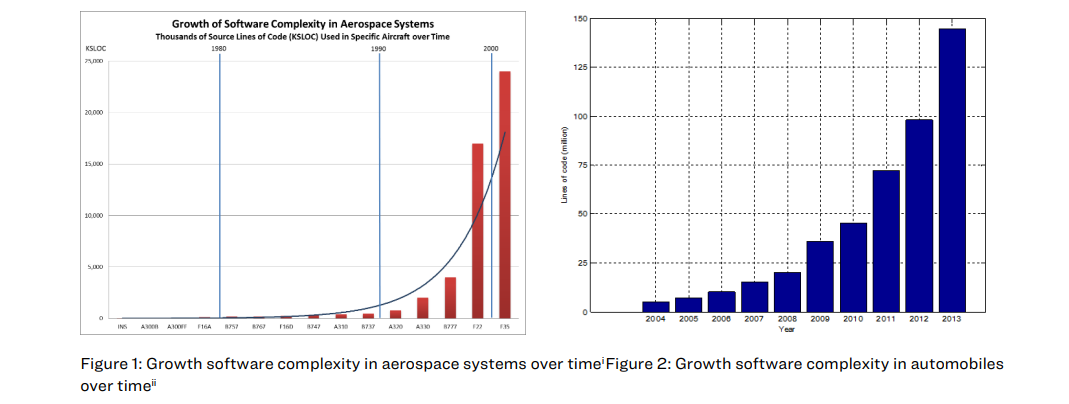
\includegraphics[width=1\textwidth]{figures/complexity.png}
  \end{center}
  \caption[Software complexity, automotive/aerospace]{Software complexity in the automotive and aerospace industry from\,\cite{moy_when_2020}}
  \label{fig:complexity}
\end{figure}
\FloatBarrier  
\end{comment}


The authors\,\cite{moy_when_2020} report security incidents which brought down AT\&T (at the cost of US\$\,60 million and long-lasting damage to the company's reputation), the \gls{FDA} warned against almost 500 thousand cardiac devices that put the patients in pain or at risk of death, and the infamous WannaCry ransomware attack that encrypted 200 thousand computers in 150 countries with a reported cost of USD\$\,8 billion.

Scherer\,\cite{scherer_engineering_2021} reports successful attacks against ``train schedule systems, entire energy grids, hospital networks, vehicular control software, and even critical aircraft systems". Scherer notes that security needs to be built into the software development process instead of being an add-on or an afterthought. Scherer also notes the ``continuously increasing rate of bugs with increasing project size amongst other factors in long-lived projects" and ``a slow turnaround time" for software improvement (1 to 10 years) causes problems to pile up.

Regarding security, the software developer also faces a series of asymmetries\,\cite{chapman_adacore_2018}, in capability (the attackers skills do not grow linearity), in efforts, knowledge and impact (the destructive impact of security failures are unpredictable). Scherer notes that any defect is guaranteed to be exploited when discovered as malicious actors systematically screen for issues. As a result, the risk that said defect is found the attacker is much higher than detection during testing\,\cite{scherer_engineering_2021}.


\section{Sustainability considerations}

Sustainability is an important concern while developing technology or advocating for its use. When it comes to the use of programming languages, considering energy consumption is essential and in line with SGD development goals 9 -- Industry, Innovation and Infrastructure --, 12 -- Responsible Consumption and Production -- and 13 -- Climate Action --\cite{noauthor_envision2030_nodate}. As studied by Pereira \etal\,\cite{pereira_energy_2017}, Ada and Rust energy consumption are comparable to C, and both languages are a good choice for energy-conscious development when it comes to various aspects, such as time, memory, and energy usage. This point is defended by companies such as AWS\,\cite{miller_sustainability_2022}, which pinpoints the increasing demand for data consumption and processing, emerging demand for \glsxtrshort{IoT} and ML applications. Broad adoption of energy-efficient programming languages could greatly reduce the energy consumption of computing by 50\%\cite{miller_sustainability_2022}.

\section{Problem}
\label{sec:problem}

Research and technical blogs recommend that programmers use memory-safe languages for new projects. They also recommend being extremely careful when using \glsxtrfull{FFI} as the boundary between two programming languages, as assumptions on both sides may not hold. 

\textbf{While frameworks and guidelines exist for C/C++, how is this implemented practically when programmers or organizations want to combine two well-known memory-safe languages?}

\subsection{Assignment provider and objective}

The research project is conducted in cooperation between Ferrous Systems and AdaCore. Both companies are engaged in an effort to provide a certified version of the Rust compiler through the Ferrocene initiative\,\cite{noauthor_ferrocene_2023}. This initiative would greatly benefit the \gls{safety-critical} industry by bringing Rust guarantees to software that \emph{should never} fail.

% Research Question
\subsection{Research question}
\label{sec:researchQuestion}

What are the best practices for secure bindings between Rust and SPARK code?

Sub questions: How can we ensure that \first \gls{memory-safety}, \Second \gls{type-safety}, and \third \gls{ownership} are maintained in these bindings?

\subsection{Hypothesis}
We hypothesize that the internal coherency of both languages can be maintained if we can provide recommendations for the safe use of combined Rust/SPARK code.

\subsection{Objectives}
The tasks must be fulfilled to answer the research question:
\begin{enumerate}
    \item Write a series of control study programs that examine the memory safety, type safety, and ownership of Rust and SPARK code when combined.
    \item Use a circular buffer library, which is implemented in both Rust and SPARK\,\cite{munns_bbqueue_2022,chouteau_bbqueue_nodate}, as a larger code base to experiment with bindings between the two languages
    \item Use the information gathered from the control study programs and the BBqueue library to identify good practices for bindings between Rust and SPARK code.
\end{enumerate}


\section{Purpose}
%\sweExpl{Syfte}
%\sweExpl{Skilj på syfte och mål! Syfte är att förändra något till det bättre. I examensarbetet finns ofta två aspekter på detta. Dels vill problemägaren (företaget) få sitt problem löst till det bättre men akademin och ingenjörssamfundet vill också få nya erfarenheter och vetskap. Beskriv ett syfte som tillfredställer båda dessa aspekter.\\
%Det finns även ett syfte till som kan vara värt att beakta och det är att du som student skall ta examen och att du måste bevisa, i ditt examensarbete, att du uppfyller examensmålen. Dessa mål sammanfaller med kursmålen för examensarbetskursen. 
%}
%\generalExpl{State the purpose  of your thesis and the purpose of your degree project.\\
%Describe who benefits and how they benefit if you achieve your goals. Include anticipated ethical, sustainability, social issues, etc. related to your project. (Return to these in your reflections in Section~\ref{sec:reflections}.)}

The purpose is to provide safe and practical recommendations that could be used by organizations or individual programmers, that are orienting themselves toward memory-safe languages.

\section{Goals}
%\sweExpl{Mål}
%\sweExpl{Skilj på syfte och mål. Syftet är att åstakomma en förändring i något. Målen är vad som konkret skall göras för att om möjligt uppnå den önskade förändringen (syfte). }

%\generalExpl{State the goal/goals of this degree project.}

The goal of this project is to study the safe combination of Rust and SPARK and provide guidelines. This has been divided into the following three sub-goals:

\begin{enumerate}[leftmargin=*, label=\textbf{Subgoal \arabic*}, ref={Subgoal \arabic*}]
\item\label{sg:selectdatatypes} Select appropriate existing data types for control studies.
\item\label{sg:safebindings} Implement control studies in a series of safe bindings.
\item\label{sg:providesafebindings} From lesson learned from \ref{sg:safebindings}, provide safe binding in a more complex library.
\end{enumerate}

%\generalExpl{In addition to presenting the goal(s), you might also state what the deliverables and results of the project are.}

\section{Research Methodology}
%\sweExpl{Undersökningsmetod}
%\sweExpl{Här anger du vilken vilken övergripande undersökningsstrategi eller metod du skall använda för att försöka besvara den akademiska frågeställning och samtidigt lösa det e v ursprungliga problemet. Ofta kan man använda ”lösandet av ursprungsproblemet” som en fallstudie kring en akademisk frågeställning. Du undersöker någon intressant fråga i ”skarpt” läge och samlar resultat och erfarenhet ur detta.\\
%Tänk på att företaget ibland måste stå tillbaka i sin önskan och förväntan på projektets resultat till förmån för ny eller kompletterande ingenjörserfarenhet och vetenskap (ditt examensarbete). Det är du som student som bestämmer och löser fördelningen mellan dessa två intressen men se till att alla är informerade. 
%}
%\generalExpl{Introduce your choice of methodology/methodologies and method/methods – and the reason why you chose them. Contrast them with and explain why you did not choose other methodologies or methods. (The details of the actual methodology and method you have chosen should be in methods. Note that in Chapter~\ref{ch:methods}, the focus could be research strategies, data collection, data analysis, and quality assurance.)\\
%In this section you should present your philosophical assumption(s), research method(s), and research approach(es).}
The objective of this thesis is to procure a series of recommendations ("\textit{Do's}") that can be applied, for example, to create an automated tool for bindings on the model of \texttt{bindgen}\footnote{As a reminder, bindgen is a binding tool that generates bindings between Rust and C.}\,\cite{noauthor_bindgen_2022}. The languages analyzed in this thesis have richer types than C, and the goal is to take advantage of their expressivity. Both languages also implement type safety and ownership, and we study how those are passed or conserved through \gls{FFI}.

The binding is considered correct if the data is correctly passed and no memory error is found \texttt{valgrind} - this does not prove complete correctness but rather the absence of memory error. But our goal is to pass the correct type through the \gls{FFI} barrier, and rely on both languages' guarantees once the \gls{FFI} frontier is passed. 

The method chosen is manually doing those bindings through control studies and analyzing them with the help of the documentation for each type as well as memory tools to ensure the binding is correct and that there is no memory leak. 

This method is reliable and appropriate as big programs are built from smaller modular pieces. In addition, \gls{FFI} research is carried out from control studies in surveyed literature. Possible issues, including safety issues, are demonstrated with the help of control studies. Control studies allow replicating the necessary complexity that is needed for illustration purposes. Control studies also allow full control over layout and alignment when passing chosen data types and data structures.
Small control study programs are useful when illustrating best practices for memory safety, type safety, and studying how ownership s transferred or maintained.
Control study programs can provide a foundation for automatic tooling.

After the control studies are performed, an additional experiment is executed with a BBqueue, a complex library available in both languages. Porting BBqueue allowed to implement most of the "lesson learned" through the control studies.


\section{Delimitations}
%\generalExpl{Describe the boundary/limits of your thesis project and what you are explicitly not going to do. This  helps you bound your efforts – as you have clearly defined what is out of the scope of this thesis project. Explain the delimitations. These are all the things that could affect the study if they were examined and included in the degree project.}

This thesis will go through manual bindings for increasingly complex types and will not implement an automated tool, which is future work.

\section{Structure of the thesis}
%\sweExpl{ Rapportens disposition}
~\Cref{ch:background} presents relevant background information about Rust and SPARK, and talks more about memory safety.  
~\Cref{ch:relatedworks} discuss related works when it comes to \gls{FFI}.  \Cref{ch:methods} presents the methodology and method used to solve the problem. ~\Cref{ch:resultsAndAnalysis} discuss the outcome of the experiments, and ~\Cref{ch:conclusionsAndFutureWork} present possible expansion of this work.


%\setglossarysection{section}
% The following line removes the glossary title.
\renewcommand{\glossarysection}[2][]{}
% Add every thing from this glossary
%\glsaddall[types={introductiongloss}] 
\printglossary[type=introductiongloss, style=mydefs, 
%toctitle={Terms in the introduction}, 
%title={Terms in the int• The statistic tool is available here.roduction}
]


\cleardoublepage\chapter{Background}
\label{ch:background}

This thesis covers the interaction of Rust and SPARK and which safety guarantees are retained when both languages are combined. Both languages implement \gls{memory-safety} but combining them in the same program requires clear recommendations. 

The background is composed of two parts. 
In Part 1, we present a 
high-level description of Rust and SPARK(\Cref{sec:rust_and_spark}), and what makes them desirable programming languages in terms of memory safety, \gls{type-safety}, as well as the concept of \gls{ownership} they both implement.

In Part 2, we discuss (\Cref{sec:software_safety}) \gls{memory-safety} in software and why the industry and researchers believe safe languages are considered to be a solution to common \gls{memory-error}s and attacks. In this part, historical memory errors and attacks are discussed to understand the protection offered by safe languages. 

\section{Background: Rust and SPARK}
\label{sec:rust_and_spark}

This section covers Rust and SPARK and describes what makes them memory safe according to the literature and their official documentation. This section explains why those two languages are relevant for \gls{safety-critical} industries and for software safety.


\subsection{Rust}

Rust was designed as a systems programming language\,\cite{mergendahl_cross-language_2022}, to interact with other low-level languages. Rust focuses on speed, \gls{memory-safety}, and concurrency. Thus, Rust is multi-paradigm and combines features from imperative \textit{and} functional programming. It is fully open-source and has a six-week release cycle, with backward compatibility guaranteed\,\cite{poveda_ruiz_bounded_2019,noauthor_rust_nodate}. Rust is characterized by its ``strong performance and safety properties". In addition, the language combines a strong type system enforced at compile-time, and other compile-time checks, to prevent ``large classes of memory bugs"\,\cite{mergendahl_cross-language_2022}. Furthermore, Rust ensures spatial safety by performing compile-time checks for statically-sized objects. For dynamically sized objects, instructions are passed to the binary, to delay those checks until runtime.

For temporal safety, Rust relies on its concept of ownership --- a concept shared by SPARK. As described by Mergendahl \etal\,\cite{mergendahl_cross-language_2022}, Scherer\,\cite{scherer_engineering_2021}, and Poveda Ruiz\,\cite{poveda_ruiz_bounded_2019} as well as the official documentation\,\cite{noauthor_rust_nodate}, a unique owner for a value can exist at a time and the value is destroyed when the unique owner goes out of scope.  This implies that when a value is destroyed, the reference is nullified, without the need for garbage collection. The Rust compiler adds lifetimes to all values, which is a ``tag" guaranteeing the value is still valid. The borrow checker ensures that no value outlives its lifetime.
 
To relax this strictness, Rust can temporarily transfer ownership, known as borrowing. More importantly, Rust allows one mutable reference \inlinecode{\& mut T} or multiple immutable references to co-exist \inlinecode{\&T} simultaneously --- these two scenarios are exclusive. This  protects against type-related errors at compile-time, as rustc (the rust compiler) warns of any error. An example of code\footnote{A note on special syntax: \texttt{!} is used to use a macro, here is a \texttt{Vector}. \texttt{\{:?\}} is used to print variables in \texttt{Debug} format.} that shifts ownership is shown in \Cref{lst:rust_ownership}.

\begin{listing}[!ht]
\begin{minted}[fontsize=\footnotesize]{rust}
// a is a vector, it is heap-allocated
let a = vec![1, 2, 3]; 
// ownership of a is moved to b
let b = a;             
println!("b: {:?}", a);
\end{minted}
\caption[Rust code showing ownership]{Rust code showing ownership}
\label{lst:rust_ownership}
\end{listing}
%\FloatBarrier

In addition, Rust’s type system statically rules out data races. At its heart, the Rust type-system has the concept of ownership. In the Rust ownership system, many aliases can exist to a place in memory, but only one alias can give mutable access, that the capacity to write to this place in memory. If ownership is shared between many aliases, then those aliases can only read the contents of this place in memory. The restrictions linked to borrowing ensure that a value is unable to exist in memory without an owning variable in the same scope, and it is impossible to modify a variable from different threads, preventing data-races\,\cite{poveda_ruiz_bounded_2019,noauthor_rust_nodate}\footnote{There are of course ways to implement thread safety such as channels or atomic reference counters (\texttt{Arc} in Rust terminology) but this is a general overview.}. 

The system of ownership is not applied to simple types as the compiler knows their size at compile-time. Those types are known to implement the \texttt{Copy trait}. This trait means that the compiler can copy those types \emph{without} needing to transfer ownership. Some simple types implementing the copy traits are integers, for example, ``i32" or ``u64". Those types are called \gls{copy-type}.

Rust allows unsafe operations that are fenced by the keyword \texttt{unsafe\{\}}. Inside unsafe brackets, operations such as raw pointer manipulation, or initialization of unsafe objects are possible, under the programmer's responsibility. Unsafe blocks are used mainly to interact with low-level code.

Rust does not implement exceptions, but has an error management system, distinguishing between recoverable and unrecoverable errors. Recoverable errors can be managed by the program, while unrecoverable errors make the program stop and unwind the stack --- resulting in a so-called \texttt{panic}. The programmer decides when an error is handled gracefully and when the program should panic.

In the somewhat contrived  example shown in \Cref{lstlisting:data_race}, we see that the compiler does not accept modification of a global variable from different threads. The compiler warns about aliasing violations or potential data races that cause undefined behavior.
\begin{listing}[!ht]
\begin{minted}[
%frame=lines,
framesep=2mm,
baselinestretch=1.2,
fontsize=\footnotesize,
linenos
]{rust}
static mut SHARED: i32 = 0; // Global scope
fn main() {
   let cls = thread::spawn(move || {
        for _ in 0..10000 {
        // aliasing violation happens here!
            SHARED += 1;
        }
   });
   for _ in 0..10000 {
      SHARED += 1;
   }
}
\end{minted}
\caption[Rust code showing aliasing violations]{Rust code showing aliasing violations}
\label{lstlisting:data_race}
\end{listing}
\FloatBarrier

\Needspace*{5\baselineskip}	
In contrast, if we frame the variable ``SHARED" inside \texttt{unsafe} blocks, the program compiles and runs, and prints all possible results between 100000 and 200000, as expected from a data race. This is an example of what \texttt{unsafe} allows the programmer to do: more freedom but it makes Rust as memory-safe as any C/C++ program.

\begin{listing}[!ht]
\begin{minted}[
framesep=2mm,
baselinestretch=1.2,
fontsize=\footnotesize,
linenos
]{rust}
    let cls = thread::spawn(move || {
        for _ in 0..100000 {
            unsafe {
                SHARED += 1;
            }
    // ...
        unsafe {
            SHARED += 1;
        }
    //...
    unsafe {
        print!("Shared {shared}");
    }
}
\end{minted}
\caption[Rust code showing a data race]{Rust code showing a data race }
\label{lstlisting:data_race2}
\end{listing}
\FloatBarrier



\subsection{Ada}

Ada is a high-level programming language, designed for long-term applications that should not be dependent on software updates -typically the safety-critical industry. It was developed in the early 1980s and has a syntax inspired by the Pascal language family.
Chapman and Moy\,\cite{chapman_adacore_2018} list some of Ada's advantages. First, its syntax protects from assignment and comparison (a well-known C problem!) as well as the unintentional use of \texttt{NULL} or the dangling else problem. In addition, there is no explicit use of pointers and its strong typing system prevents confusion or abusive type promotion. Furthermore, it has many features for concurrency.

Ada has strong type safety as in Rust. Additional constraints can be imposed with subtypes or bounds. This ensures at compile-time that data is only used in ways that are consistent with its declared type and that type-safety is not violated.

 \begin{listing}[!ht]
    \begin{minted}[
        frame=lines,
        framesep=2mm,
        baselinestretch=1.2,
        fontsize=\footnotesize,
        linenos
    ]{ada}
    -- those are not the same type, and it is impossible
    -- to assign those interchangeably.
    type My_int is range -1 .. 20;
    type My_int2 is range -1 .. 20;
   
   -- same here!
   subtype MyInteger1 is Integer range 0..10;
   subtype MyInteger2 is Integer range 5..15;
\end{minted}
\caption[Ada/SPARK code showing type guarantees]{Ada/SPARK code showing type guarantees}
\label{lstlisting:spark_datatypes}
 \end{listing}

\subsection{SPARK}

%\gls{safety-critical}

SPARK refers to a set of tools for verification as well as the language name.
SPARK allows formal verification of code to provide guarantees that would not be achieved otherwise at multiple levels of assurance, which can be integrated into development processes (Moy, in direct conversation). The language was designed to be the largest subset of Ada that was ``still amenable to simple specification and sound verification", and as such, the use of pointers (which permits aliasing!) was not a part of the language until fairly recently \footnote{at the time of writing, 2014}\,\cite{jaloyan_safe_2017, dross_using_2019}.

 SPARK supports, amongst other features, basic data, control flow analysis, ineffective assignments, and exhaustive detection of uninitialized variables. To ensure the safety and security of software systems, SPARK provides support for mathematical proofs. These proofs can be used to demonstrate the absence of runtime exceptions, verify the fulfillment of security and safety properties, or establish that the software follows its specifications and has the required behavior\,\cite{noauthor_spark_nodate}.
 
Carré and Garnsworthy\,\cite{carre_spark_1990} describe the rationale behind the design of SPARK, highlighting a number of key requirements that the language must meet to be effective in safety-critical programming contexts. These include being logically sound and free of ambiguities, having a simple and formal definition, maintaining expressive power to support rigorous program development and faithful representation of abstractions, prioritizing security and reliability to ensure that errors are not tolerated in safety-critical contexts, and finally, the ability to be verifiable.

SPARK is compiled with the Ada compiler, (GNAT is used in the experiments in this thesis) but it has in addition the SPARK checker. SPARK verifies contracts are always upheld, insuring no runtime error, proving for example that no division by zero is possible or that the result of an increment is always bigger than the number sent to the program. In addition, SPARK ensures thread safety via synchronized objects (Scherer\,\cite{scherer_engineering_2021}, SPARK resources\,\cite{noauthor_spark_nodate}).

As an example from AdaCore documentation (\Cref{lstlisting:spark_illegal_transfer}), this program is legal in Ada but illegal in SPARK, as the operation on \texttt{X} is not benign, meaning that we are trying to make an assignment to the contents of a pointer whose \gls{ownership} has been moved to \texttt{Y}. Once \texttt{Y} has ownership of the data contained in \texttt{X}, it becomes impossible to manipulate \texttt{X}.

\begin{listing}[!ht]
    \begin{minted}[
    %frame=lines,
    framesep=2mm,
    baselinestretch=1.2,
    fontsize=\footnotesize,
    linenos
    ]{ada}
    procedure Ownership_Transfer is
       type Int_Ptr is access Integer;
       X     : Int_Ptr;
       Y     : Int_Ptr;
       Dummy : Integer;
    begin
       X     := new Integer'(1);
       X.all := X.all + 1;
       Y     := X;
       -- legal, ownership pertains to Y
       Y.all := Y.all + 1;  
       -- illegal, trying to access a variable through X,
       -- which was moved. No further operations, 
       -- assignment and transfer are possible.
       X.all := X.all + 1;  
       X.all := 1;          
       Dummy := X.all;      
    end Ownership_Transfer;
    \end{minted}
    \caption[Illegal ownership transfer in SPARK]{Illegal ownership transfer in SPARK}
    \label{lstlisting:spark_illegal_transfer}
\end{listing}

Pointer ownership in SPARK took inspiration from Rust\,\cite{dross_using_2019}, with some differences. In SPARK, only read aliasing is allowed, as per the Concurrent-Read-Exclusive-Write (CREW) model \cite{moy_proof_2019}. SPARK checks the absence of aliasing on write at the call site. Pointer assignment operates as a transfer of ownership, where the source object loses permission to the underlying object as per \Cref{lstlisting:spark_illegal_transfer}. Once ownership is transferred, the original owner is not valid. Begning aliasing, or local handles on data with pointers ``borrow" for read, called \emph{observability}.


\subsection{Summary on Rust and SPARK}

The concept of type safety and ownership, and why these traits are considered desirable in safe programming languages like Rust and SPARK, have been covered in detail. Those traits are their use of strong \gls{type-safety} and ensuring \gls{memory-safety} through \gls{ownership}. This reduces the probability of \gls{memory-safety} errors as SPARK does not fail at runtime and the Rust compiler maintains its guarantees as long as the programmer does not use \texttt{unsafe} wrongly.

%\newpage

\section{Background: Software Safety}
\label{sec:software_safety}

The literature around the state of software security generally agrees about the threats caused by memory-safety issues and the underlying reasons for those threats, namely unsafe languages. 

\subsection{Memory safety}

Skezeres \etal\,\cite{szekeres_sok_2013} (in ``SoK: Eternal War in Memory") and Pal \etal\,\cite{pal_memory_2016} (in ``Memory Corruption-Basic Attacks and Counter Measures") define \gls{memory-safety} in terms of protection against \gls{memory-error}s. 
In the C++ standard, writing out-of-bounds of an array, dereferencing null pointers, or reading uninitialized variables results in undefined behavior. Buffer overflows (writing outside of the allocated space in memory), double-frees (freeing the memory twice), and use after free (accessing a memory that has been freed before) are very common errors\,\cite{szekeres_sok_2013,scherer_engineering_2021}. 
These errors can be leveraged into full-fledged attacks, as ``every exploit starts by triggering a memory error"\,\cite{szekeres_sok_2013}. The attack process is two-fold. The first is to make a pointer invalid, and the second is dereferencing this invalid pointer. Attackers can exploit either dangling pointers (\ie temporal errors) or an out-of-bound pointer (\ie a spatial error). These attack techniques can be combined and chained for successful exploitation. 
%as illustrated in detail in \Cref{fig:sok}.

\Needspace*{17\baselineskip}
\subsection{The `Memory Wars"}.

C/C++ are especially susceptible to \gls{memory-error}s, because of the freedom they give to the programmer. Szekeres \etal\,\cite{szekeres_sok_2013} call the \gls{memory-corruption} bugs in low-level languages ``one of the oldest problems" in security. Memory errors have been exploited for 30 years, while real-world exploits prove that protections can always be defeated. The authors established that not only does a completely secure system not exist, but protection mechanisms never achieve wide adoption by the software engineering community. The reason is that protection mechanisms present a significant overhead, in terms of performance (\eg garbage collectors are costly in systems relying on speed, not even to mention changing the programming language, and the trade-off is not worth the benefit of the protection) or more simply the cost of replacing billions of lines of existing C/C++ is too expensive. According to Skezeres \etal\,\cite{szekeres_sok_2013} the issues may be that the protection is not robust enough or there exist problems of incompatibility with legacy code and dependencies.

\begin{comment}
    
  \begin{figure}[!ht]  \centering 
\includesvg[inkscapelatex=false, scale=0.4]{figures/figuressvg/redrawn_memory_attack.svg}
\caption{Redrawn figure}
\end{figure}
\FloatBarrier  




\begin{sidewaysfigure}[!ht]
  \begin{center}
    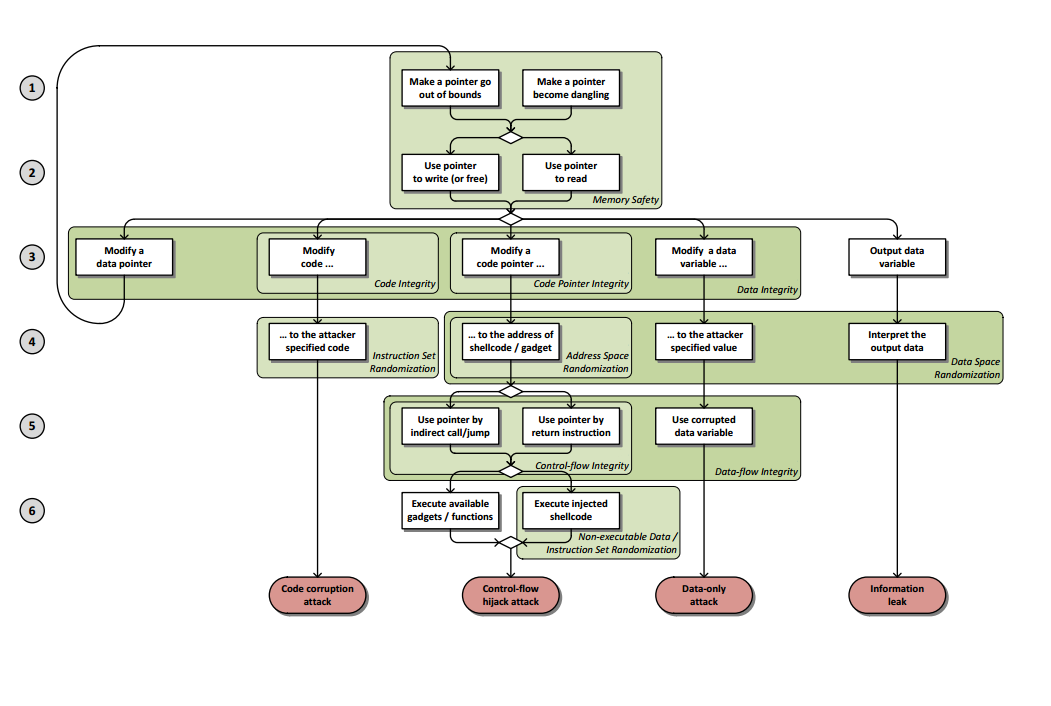
\includegraphics[width=0.8\textwidth]{figures/sok.png}
    %\includesvg{figures/sok.svg}
  \end{center}
  \caption[Attack model demonstrating four exploit types and policies mitigating the attacks in different stages by Szekeres \etal\,]{Attack model demonstrating four exploit types and policies mitigating the attacks in different stages by Szekeres \etal\,\cite{szekeres_sok_2013}  \textcopyright2013 IEEE}
  \label{fig:sok}
\end{sidewaysfigure}

\end{comment}

To mitigate these problems, various tools have been introduced\,\cite{mergendahl_cross-language_2022}. Dynamic analysis tools observe the program while it is running, while static analysis tools analyze the source code. Such tools are for example Valgrind, sanitizers (dynamic analysis), or the Clang static analyzer. Even if writing analysis tools is, to say the least, ``non-trivial"\,\cite{scherer_engineering_2021}, some authors studied in the frame of this thesis wrote their own (FFIChecker by Li \etal\,\cite{li_detecting_2022} and Scherer who participated to the project Miri\,\cite{noauthor_miri_2023}). Tools have limitations: dynamic analysis tools are time-consuming and specific to the input, and static analysis tools have false positives\,\cite{li_improving_2014}.
Unfortunately, those tools provide very limited protection, in part because the software engineering community is facing professionalization and an increase in complexity from the attacking side\,\cite{scherer_engineering_2021, chapman_adacore_2018}. 
According to Mergendahl \etal\,\cite{mergendahl_cross-language_2022}, ``sanitizers suffer from coverage limitations", with many missed bugs as a consequence, while ``enforcement-based exploit mitigation techniques" can still allow attacks that do not violate their policies as they are ``relaxed enough", and randomization techniques remain susceptible to information leakage.
\FloatBarrier



\subsection{The monopoly of C/C++}

Both C/C++ are considered as building bricks of modern software, in systems programming and embedded because of the performance they offer, as argued by Mergendahl \etal and Scherer \,\cite{mergendahl_cross-language_2022, scherer_engineering_2021}. Both C/C++ are also prevalent in embedded systems (Moy and Aiello\,\cite{moy_when_2020} Chapman and Moy\,\cite{chapman_adacore_2018}). Renouncing C/C++ is equivalent to renouncing performance and losing the fine-grained control necessary to work with low-level systems.
C/C++ are by nature unsafe languages. They are designed for direct interaction with memory and can modify it without any restriction. Mergendahl \etal state that the underlying root of all evil, \gls{memory-corruption}, comes from the error-prone process of delegating all security checks to the programmer. As a consequence, developer errors introduce both spatial and temporal errors.

The inherent unsafely of C/C++ affects safe languages. By design, Rust and Ada (and its subset SPARK) were designed to interact with existing low-level applications written in C/C++, and use dependencies written in unsafe languages. 

\section[FFI in software engineering]{FFI in software engineering}

\glsxtrshort{FFI} is commonly used in systems programming languages. 
To write software with FFI in general, as well as in this thesis, it is important to follow existing guidelines\,\cite{gjengset_rust_2021, noauthor_ffi_nodate, noauthor_multi-language_nodate}. 
Those guidelines cover important points such as calling conventions (that is to say, the data representation that the compiler is expect) or symbols, which must be deterministically generated. Error management is critical, as unwinding an error through an FFI barrier is considered undefined behavior. Type matching is also an important consideration, as one language possesses no information on the representation of complicated types in another language. We consider memory management (when to keep and release ownership) which most of the time must be returned to the appropriate allocator according to guidelines\,\cite{gjengset_rust_2021}. 

In ``Improving Quality of Software with Foreign Function Interfaces using Static Analysis", Li\,\cite{li_improving_2014} covers the reason for FFI prevalence in modern software. FFI is a gluing layer that allows the connection of software written in different languages. Multi-language software seems ``prevalent and necessary"\,\cite{li_detecting_2022}: different languages have different strengths due to design choices, or rich ecosystems, or have a specific use for ``performance-critical scenarios" in a time where software development requires faster processes, higher quality, and faster time to market.

Some problems arise only in multi-language contexts as failures can be caused by wrong assumptions. ``Rust’s automatic memory management relies on it being the only entity controlling the allocation status of memory"\,\cite{mergendahl_cross-language_2022} --- but this may not be the case. Rust uses \texttt{malloc()} and shares a heap with other components of multi-language applications. So, ``Rust’s spatial memory safety can rely on bounds stored in memory which is only safe if the entire application is memory safe"\,\cite{mergendahl_cross-language_2022}.

\glsxtrfull{CLA} show, counter-intuitively, that multi-language applications are weakened by the very assumption the programmer has about combining different languages' strengths. Instead, it is each language's \emph{weakness} that threatens to become the weakest link of the application.
For example, hardened C through \gls{CFI}, prevents control-flow hijacking by checking the validity of pointers. The Rust side provides protection against the same attacks by enforcing memory safety. However, this does not make the C side memory safe, and Rust does not validate the code pointers --- it just assumes \gls{memory-safety} in the whole memory space. The attacker can take advantage of the C language weaknesses to combine memory corruption and non-validated pointers in Rust. 

Mergendahl \etal\,\cite{mergendahl_cross-language_2022}, insist that the problem is much deeper than what meets the eye. They could demonstrate control-flow hijacking, but the ``weakest link principle holds for any element of an application’s threat model that varies across languages". If one part of the code introduces code signing and validation (on the Rust side), but another part of the code does not (C libraries), then the cross-language application remains completely vulnerable to supply chain attacks.

Finally, the authors introduce the most ``insidious case of multi-language applications". The component languages can have eliminated a threat but use different assumptions. The result is that ``the combination of two safe languages itself being unsafe", a theory that is of the utmost interest in the frame of this thesis --- as both Rust and SPARK are safe languages.

The authors also underline that the cost of writing such attacks is relatively simple: while attacks on single-language code require ``new primitives", \glsxtrshort{CLA} opens a new avenue of attack reusing old vulnerabilities ``brought back to life" ---the attack that we surveyed in \Cref{sec:software_safety}, in addition to CLA specific vulnerabilities. The authors call those attacks ``revenant vulnerabilities"\,\cite{mergendahl_cross-language_2022}. 

\section{Summary}

Memory safety is a primary concern in low-level and systems programming, with constant research for its improvement (\Cref{sec:software_safety}). Ameliorating the state of affairs is challenging, in terms of cost and trade-offs.

\cleardoublepage

%\chapter[Related works: Foreign Function Interface]{Related works: Foreign\linebreak[4] Function Interface}
\chapter{Related works}
\label{ch:relatedworks}

Related works examine dependencies, language formalization, and studies around \glsxtrfull{FFI}.

\section{Dependencies}
\label{subsec:dependencies}

Safe systems programming languages can be dependent on libraries written in unsafe languages. Even if those dependencies were well tested, they still represent a safety risk. As a result, the inherent unsafely of C/C++ can affect safe languages. Rust was designed to interact with existing low-level applications written in C/C++ but can also depend on libraries written in C/C++. This is different from SPARK, which only depends on Ada, even if programmers can interface with C/C++ as any system programming language.

While the consensus is that the Rust language is excellent in reducing memory-safety issues, Evans \etal examined the actual usage of Rust by developers in their paper ``Is Rust Used Safely by Software Developers?"\,\cite{evans_is_2020} and their conclusions are somehow different. They note that \texttt{unsafe\{\}} --- a Rust keyword to do memory operations not authorized by the compiler \footnote{See more details in \Cref{sec:rust_and_spark}} is used in one-third of dependencies which are impossible to check. They believe ``propagation of unsafeness offers a challenge to the claim of Rust as a memory-safe language". In this case, Evans \etal recommend changes to the rust compiler to raise awareness in programmers when their code is rendered unsafe through dependencies. 

But Evans \etal do not quantify their findings. Li \etal (in ``Detecting Cross-Language Memory Management Issues in Rust"\,\cite{li_detecting_2022}), analyzed whether  Rust could realize its promised guarantees and found that more than 70\% of packages on \texttt{crates.io} have at least one unsafe binding. This result is based upon their looking at approximately 77,000 packages. Finally, Li \etal built a \gls{FFI}-checker tool that found only 34 bugs in 12 packages out of a sample of 984 packages. The authors consider this result of great significance (probably because of Rust's memory safety reputation) as the bugs were previously unknown and were subsequently reported by the authors in a GitHub trophy case \,\cite{li_rust-ffi-checkertrophy-case_nodate}. The relatively low number of bugs seems to strengthen the consensus around safety guarantees provided by Rust.

\section{Formalization}

Rust is an open-source project without formal specifications, contrasting with Ada and SPARK. But there are many efforts ongoing to formalize Rust. The Rust Belt\,\cite{jung_rustbelt_2018} project aims ``to equip Rust programmers with the first formal tools for verifying safe encapsulation of unsafe code". Rust Belt defines a set of rules to model Rust programs and uses those rules to prove the security of those programs mathematically. Rust Belt has demonstrated the safety of basic typing and that there is no undefined behavior in well-typed Rust \,\cite{xu_memory-safety_2021}. 

The Ferrocene language specification (a collaboration between Ferrous Systems and AdaCore\,\cite{noauthor_ferrocene_2023}) aims to document the behavior of the Rust compiler in a standardized form. The goal is to qualify a version of the Rust compiler for use by safety-critical industries.

SPARK is built upon the Ada standard ISO/IEC 8652:2012\,\cite{1400-1700_isoiec_2013}, which defines the form and meaning of programs to ensure the portability of Ada code. Specifically, SPARK Pro is a group of static analysis tools which use formal methods to verify SPARK deductively. This tool can meet several high-assurance standards, including DO-178B/C (and the Formal Methods supplement DO-333), CENELEC 50128, IEC 61508, and DEFSTAN 00-56\,\cite{jaloyan_safe_2017}.

\section{Software written with FFI}

Previous publications have found many issues when combining safe and unsafe languages, making the multi-language program weaker than the sum of their part. But even a combination of safe languages can be expected to be unsafe.

With this goal in mind, we set aside discussions on \gls{memory-safety} in single-language applications (such as Regehr \etal and Chandra \etal focusing on C\,\cite{regehr_efficient_2006,chandra_physical_1999}), and papers too tightly centered around security (such as the work on the formalization on exploits by Dullien\,\cite{dullien_weird_2020}). 

In this part, we review again the work of Mergendahl \etal\,\cite{mergendahl_cross-language_2022} whose paper was an inspiration for this thesis, Li's work on improving FFI software safety\,\cite{li_improving_2014}, Scherer work on software safety\,\cite{scherer_engineering_2021} and Li \etal\,\cite{li_detecting_2022}, who built on Mergendahl \etal work. For a formal expression of the need for linking type, we can refer to the work of Patterson and Ahmed\,\cite{patterson_linking_2017} on using richer types available in other languages and linking those types modeled in abstract compilers.

Software built with FFI layers can be listed easily\,\cite{li_improving_2014,li_detecting_2022,mergendahl_cross-language_2022}: the \gls{JNI} which glues together the \gls{JDK} and it's core systems libraries written in C and C++, the Android mobile \gls{OS} which includes a Java \glsxtrfull{VM} and a C/C++ kernel; Firefox --- studied extensively by Mergendhal \etal which is also a well-known example. The Linux kernel is integrating Rust as a core language\footnote{At the time of writing this thesis.}. The Tor project, Microsoft Windows \gls{OS}, and Google Fuchsia can also be named.

\subsection{How to evaluate quality in FFI bindings}

Li distinguishes four software quality issues caused by \glsxtrshort{FFI}: security, reliability, safety, and performance\,\cite{li_improving_2014}.

\begin{description}[labelwidth=\widthof{\textbf{Memory safety}}, leftmargin = !]
\item[\textbf{Security}] implies that an attacker is not in a position to exploit the FFI layer for security attacks. 
\item[\textbf{Reliability}]implies that the system should not behave unexpectedly because of its FFI layer(s).
\item[\textbf{Safety}] implies that multi-threaded execution is safe. This property has been studied extensively but only for uni-language systems and is not relevant for FFI. Commonly, safety issues involve deadlocks and race conditions, synchronization in threads, and data integrity. While the present thesis does not investigate multi-threading, it is important to stress that it is a core issue in FFI safety.
\item[\textbf{Performance}] Performance issues are mostly related to poor memory management (memory leaks, dangling pointers...)
\end{description}

However, independently of quality metrics, calling external code is inherently dangerous (Mergendahl \etal\,\cite{mergendahl_cross-language_2022} and Li \etal\,\cite{li_detecting_2022}). Intuitively, calling foreign code that does not present the same guarantees as a safe language should be considered dangerous. But according to the existing literature, simply the fact that our code \textbf{is} multi-language makes it dangerous, independently of which languages are bound together, even if called languages offer many guarantees. It depends on the assumption.

\subsection[A new cross-language paradigm for the programmer]{A new cross-language paradigm for\linebreak[4] the programmer}

Li\,\cite{li_improving_2014} stresses why using \glsxtrshort{FFI} is an error-prone process for the programmer. From the human perspective, it is not only expected to reason in their own language but across different languages. Some differences are straightforward, such as  type system, semantics, and syntax while some are more subtle, such as exceptions or error handling, or memory management. All of a sudden, the programmer needs to understand the nuances and complex inter-connectivity of programming languages, as well as the context that allows the apparition of specific bugs.

In a safe language such as Rust, programmers may misuse the \texttt{unsafe} abilities that are provided to them (Li \etal\,\cite{li_detecting_2022}), while any mistake at the FFI layer may corrupt Rust safety, an issue stressed by Evans \etal\,\cite{evans_is_2020}.

In other words, FFI are challenging, not only when it comes to identifying bug patterns but also in establishing solutions. In addition, programmers (and researchers) must now reason about single-language components in a multi-language context. 
For example, Java programmers tend to avoid reasoning about code interleaving and can consider native methods as black boxes\,\cite{li_improving_2014}. 
The complexity is accrued by the general lack of experience in FFI and the lack of empirical or experimental research. From the programmer and researcher side, it requires keen knowledge and comfort with both the foreign and host languages, in particular within exception and error handling, memory, type system, and thread models, as well as a deep understanding FFI interactions and the 
impact that the technique itself may have during those interactions.  In other words, FFI errors are one of the most significant causes behind memory-safety bugs in existing code bases\,\cite{li_improving_2014, patterson_linking_2017}.

\subsection{Issues from the compiler perspective}

While managing \glsxtrshort{FFI} is challenging from the human perspective, it is also not trivial for a compiler. While writing code, programmers add annotations that are an additional source for the compiler. Richer linking types are beneficial as a source of information\,\cite{patterson_linking_2017}. Mergendahl \etal\,\cite{mergendahl_cross-language_2022} also illustrate how it is inherently unsafe to use FFI in Rust. Even if Rust has rules, such as a warning that the programmer should avoid using dynamically-sized types, it still authorizes sending arbitrary data and pointers across the language barrier \footnote{just to be clear, this rule is not forcefully implemented. The compiler warns but does not prevent compilation. Sending dynamically-sized data is de facto possible}. 
And when communicating with C, this requires the \texttt{unsafe} keyword, which indicates to the compiler that the programmer is taking responsibility from the compiler to ensure that this part of the code is correct.

Additionally, Mergendahl \etal stress another aspect, namely the difference between intended/unintended interactions. Their work focuses on intended interactions, but they remind us that unintended interactions are also possible within multi-language applications sharing a heap and an address space. In other words, a new class of bugs not yet discovered await the unsuspecting programmer, which the authors leave as future work\,\cite{mergendahl_cross-language_2022}.

\subsection{FFI introduces a new class of bugs}

Bugs introduced by \glsxtrshort{FFI} are not straightforward (Li\,\cite{li_improving_2014}). They are subtle, and the lack of previous experience and tools introduces additional complexity. There is very little empirical or experimental research systematically identifying FFI bugs\footnote{At the time of writing in 2014, but other authors do not mention a strong body of research.}.

On the contrary, Li insists that the search for bug patterns particular to FFI has just begun. This search focuses on a small set of problems that concern a minority of software quality issues --- while some bugs are completely unique. This is also a point confirmed by Mergendahl \etal\,\cite{mergendahl_cross-language_2022}, as well as Li \etal\,\cite{li_detecting_2022}.

Work on Rust FFI is closely related to research done on \glsxtrshort{JNI} (Mergendahl \etal\,\cite{mergendahl_cross-language_2022}). Without entering into too many details unrelated to this thesis, one pattern causing vulnerabilities is the mishandled Java exceptions. At the time of writing (2014), this bug pattern was considered unique (Li\,\cite{li_improving_2014}), but not unique to JNI. This pattern concerned any language which allowed exceptions thrown by native components\,\cite{li_improving_2014}. Rust is known for its rich error handling management (distinguishing recoverable vs. unrecoverable errors, error propagation) and how Rust errors can be propagated to SPARK through FFI is a relevant question in the frame of this thesis. 
\subsection{Cross-Language Attacks}

When going further from \emph{mere} memory unsafety to the actual act of exploitation, Mergendahl \etal\,\cite{mergendahl_cross-language_2022}, emphasize how incompatible assumptions on different sides of the \glsxtrshort{FFI} permit attacks that are impossible in a single language context. The authors mean that the gradual integration of additional safe languages in an unsafe code base, which was assumed to improve the code base safety was in fact a problem. By doing so, the authors add a new vector of attack to the current knowledge on security, the \gls{CLA} vector. They demonstrate that the mere idea of ``incrementally hardening memory unsafe code with memory safe code can have serious flaws—beyond C/C++ hardening bypasses—if not handled properly"\,\cite{mergendahl_cross-language_2022}.

Although Rust and other safe programming languages, such as Go and Swift, are announced as being the best chance for safe software Mergendahl \etal show several examples of how exploitation is possible because of the combination of safe and unsafe languages. Furthermore, since exploitation in unsafe languages without protection are ``trivial"\,\cite{mergendahl_cross-language_2022}, the authors focus on the case where  \glsxtrshort{FFI} is bridging unsafe code with \textit{some} protection, and safe code. 


In Mergendahl \etal model \glsxtrshort{CLA} starts in a safe language (Rust), where memory safety is guaranteed. The control flow is transferred to the unsafe language to proceed to the memory corruption (where hardened C with \gls{CFI} ensures that control-flow hijacking is made impossible). The application transfer back to the safe language to execute the gadget. In summary, the unsafe language assumes [\ldots\ ] hardening (control flow integrity), which prevents control hijacking, while the safe language assumes the program is free of corruption.

The authors insist that their model while focusing on Rust and C++ for simplicity, can generalize to other safe languages. It is natural to wonder how it can generalize between safe languages such as SPARK and Rust. In their conclusions, Mergendahl \etal note that they believe their model applies to Rust and Go. Those two safe languages have different strategies around memory safety --- that is lifetime management and garbage collection. If a system combining both disagree, double frees and use after frees are still possible, which opens the door to other non-obvious vulnerabilities\,\cite{mergendahl_cross-language_2022}.

Mergendahl \etal successfully illustrate that any FFI established without ``extreme care"\cite{mergendahl_cross-language_2022} can lead to artfully crafted exploits, where the classic control-flow hijacking was impossible before. They show that the thread model for a multi-language application is the ``union of the threat models of the constituent languages"\cite{mergendahl_cross-language_2022}. Does this bring the state of knowledge to where we were with C/C++, where the programmer was responsible for securing the program?

\section{Summary}

Ensuring software security can be challenging, even in languages with strong safety guarantees. One reason is that dependencies can introduce potential vulnerabilities, and another reason is that programmers can still call unsafe code. However, the SPARK is formally verified, and the Rust community is actively working towards formal verification as well. Adhering to established guidelines and specifications is the first step to ensuring security.

Multi-language applications with \glsxtrshort{FFI} open new vectors of attacks and resuscitate old vulnerabilities. This is still true when combining two safe languages with different memory assumptions. 
There is ongoing research around FFI, as it is a complicated subject for the programmer and the compiler. In addition, debugging FFI software is a complex and uncharted territory. The most effective tool is static analysis\,\cite{li_improving_2014}, which requires expertise from the programmer.
This reinforces the need for safe guidelines when building multi-language applications.


\cleardoublepage
\chapter[Methods: Control studies and BBqueue]{Methods: Selection process for control studies and\linebreak[4] presentation of the BBqueue library}
\label{ch:methods}
%\sweExpl{Metod eller Metodval}
%\generalExpl{This chapter is about Engineering-related  content, Methodologies and Methods.  Use a self-explaining title.\\The  contents and structure of this chapter change with your choice of  methodology and methods.}


%\generalExpl{Describe the engineering-related contents (preferably with models) and the research methodology and methods that are used in the degree project.\\
%Give a theoretical description of the scientific or engineering methodology  you are going to use and why have you chosen this method. What other methods did you consider and why did you reject them?\\
%In this chapter, you describe what engineering-related and scientific skills you are going to apply, such as modeling, analyzing, developing, and evaluating engineering-related and scientific content. The choice of these methods should be appropriate for the problem. Additionally, you should be conscious of aspects relating to society and ethics (if applicable). The choices should also reflect your goals and what you (or someone else) should be able to do as a result of your solution --- which could not be done well before you started.}


\begin{comment}
(1) Vilken process skall användas för konstruktion av lösningen och vilken process skall kopplas till denna för att svara på undersökningsfrågan?\\
(2) Hur och vilket resultat (storheter) skall presenteras både för att redovisa svar på undersökningsfrågan (resultatkapitlet i denna rapport) och redovisa resultat av problemlösningen (prototypen, ofta dokument som bilagor men vilka dokument och varför?).\\
(3) Vilken teori/teknik skall väljas och användas både för undersökningen (taxonomi, matematik, grafer, storheter mm)  och  problemlösning (UML, UseCases, Java mm) och varför?\\
(4) Vad behöver du som student leverera för att uppnå hög kvaliet (minimikrav) eller mycket hög kvalitet på examensarbetet?\\
(5) Frågorna kopplar till de följande underkapitlen.\\
(6) Resonemanget bygger på att studenter på hing-programmet ofta skall konstruera något åt problemägaren och att man till detta måste koppla en intressant ingenjörsfråga. Det finns hela tiden en dualism mellan dessa aspekter i exjobbet.
\end{comment}

This chapter provides an overview of the research method and experimentation, as well as information for reproducibility. 

%Section~\ref{sec:researchProcess} describes the research process. Section~\ref{sec:researchParadigm} details the research paradigm. 
%Section~\ref{sec:dataCollection} explains the selection of data types for the control studies. Section~\ref{sec:experimentalDesign}
%describes the experimental design. 
%\Cref{sec:methodBBQueue} covers our work on BBQueue. Finally, Section~\ref{sec:systemDocumentation}
%describes the system to ensure reproducibility.

\section{Research Process}
\label{sec:researchProcess}

Figure~\ref{fig:researchprocess} decomposes the steps to carry on this project. 

%https://tex.stackexchange.com/questions/116621/tikz-flow-chart-questions

\begin{figure}[ht!]
    \centering
    \scalebox{0.9}{
    \begin{tikzpicture}
    [node distance=.8cm,
    start chain=going below, %font=\large,
    tuborg/.style={decorate, decoration={brace, amplitude=3pt}, line width=1mm},
    tubnode/.style={midway, right=2pt, align=left, font=\large, text width=4cm, xshift=4mm},
    ]
    % group 1
         \node[punktchain, join, draw=black,fill=color1bg_fill] (lit){Literature study};
         \node[punktchain, join, draw=black,fill=color1bg_fill] (consult){Consultation with experts};
         \node[punktchain, join, draw=black,fill=color1bg_fill] (scope){Scope limitation};  
    % group 2
         \node[punktchain, join, draw=black,fill=color2bg_fill] (typselec){Type selection};
         \node[punktchain, join, draw=black,fill=color2bg_fill] (stats){Statistics};
    % group 3
         \node[punktchain, join, draw=black,fill=color3bg_fill] (cs){Control studies};
         \node[punktchain, join, draw=black,fill=color3bg_fill] (analys){Analysis};   
         \node[punktchain, join, draw=black,fill=color3bg_fill] (memver){Verification of correctness};   
    % group 4
         \node[punktchain, join, draw=black, fill=color4bg_fill] (bbq){BBQueue implementation};
    %% No. 1
    \draw[tuborg, decoration={brace}] let \p1=(lit.north), \p2=(scope.south) in
        ($(3, \y1)$) -- ($(3, \y2)$) node[tubnode] {Preparation};
    %% No. 2
    \draw[tuborg, decoration={brace}] let \p1=(typselec.north), \p2=(stats.south) in
        ($(3, \y1)$) -- ($(3, \y2)$) node[tubnode] {Types selection};
    %% No. 3
    \draw[tuborg, decoration={brace}] let \p1=(cs.north), \p2=(memver.south) in
        ($(3, \y1)$) -- ($(3, \y2)$) node[tubnode] {Control studies};
    %% No. 4
    \draw[tuborg, decoration={brace}] let \p1=(bbq.north), \p2=(bbq.south) in
        ($(3, \y1)$) -- ($(3, \y2)$) node[tubnode] {Real-world \\ implementation};
    \end{tikzpicture}}
  \caption{Research Process}
  \label{fig:researchprocess}
\end{figure}


The research process is constituted of four steps:

\begin{enumerate}[leftmargin=*, label=\textbf{Step \arabic*}, ref=Step \arabic*] %labelindent=1em for indent
    \itemsep0em
    \item \label{x:s1} Preparation: planning the experiments and delimiting the scope, including setting all appropriate tooling and environment for both Rust and SPARK ecosystems,
    \item \label{x:s2} Type selection: choosing data types for control studies,
    \item \label{x:s3} Control studies: perform the control studies, and
    \item \label{x:s4} Application: apply the learning from the control studies in a real-world setting.
\end{enumerate}
\FloatBarrier

\section{Research Paradigm}
\label{sec:researchParadigm}

Three paradigms are used. 

Firstly, this project is hypothesis-driven. The hypothesis is that the internal coherency of both languages can be maintained if we can provide
recommendations for the safe use of combined Rust/SPARK code, and this is a hypothesis that we strive to confirm.


Secondly, the qualitative research paradigm is applied when carefully selecting data types that allow the exploration of safe bindings.


Thirdly, the empirical research paradigm is also used. After guidelines are established through control studies, an applied experiment consists of following said guidelines to a larger code base. This step is appropriate as this is an experiment with real-life setting, and bugs and errors are expected to arise. This experiment is relevant as it is a first step in reproducibility and generalization.



\section{Choice of datatypes for control studies}
\label{sec:dataCollection}

The research question that was raised early in this process is how to select useful Rust and SPARK types for analysis. 
With the tool described below, we could reply to the preliminary research question and select data types that are stack and heap objects, and mostly references/pointers. 

A simple regex counter was created to analyze 17 Rust code bases\footnote{\href{https://github.com/Dajamante/stat_ada_rust_code}{Rusty Regex Types Counter}}, including the Rust compiler, and three open-source code bases in SPARK for a total of 1,861 k\gls{LOC}. The selected data types are a series of stack and heap objects, which were chosen based on the results of the statistical tool that identified widely used types in Rust and SPARK projects. 

With that tool and expert advice, we identified which types are widely used and relevant in Rust and SPARK projects (\cref{sec:stats}).

\subsection{Statistic tool}
\label{sec:stats}


The program counts occurrences of different patterns with Regex in the code bases, including numbers, arrays, references, strings, and various heap-allocated types. The detailed patterns and scripts will be provided in \Cref{sec:systemDocumentation}.

\texttt{cloc 1.9} counted 26,754 Rust files (1,862 k\gls{LOC}) in popular and qualitative Rust repositories. It covered 504 Ada files in open-source SPARK repositories, totalizing 27 kLOC.

The detailed list of regexes used for statistics is available in \Cref{sec:regexes}.

\subsection{Reliability and validity of the statistics}

The data is collected via file parsing and \texttt{Regex} patterns\footnote{Using the Regex Rust crate \href{(documentation)}{https://crates.io/crates/regex}}. 

One source of error can be that some data types can appear in comments instead of the code. This results in the counts being potentially higher than the actual numbers; however, a manual inspection of some matches indicates that the extent of numbers in comments is limited, and the numbers are fairly close to the actual occurrences of the counted type.


Another source of error is that while the regex covers the most common cases, they do not cover edge cases.
%When it comes to Rust mutable and immutable references, admittedly references can point at any data structure, i.e, a \inlinecode{struct AStruct} can be declared and then referred by a number of \inlinecode{\&AStruct}. But this does not mean that we count the same object several times, rather then we study the use of references and how ownership is transmitted. 

%The presence of many references and pointers (\inlinecode{\&mut T} and \inlinecode{\&T}, as well as \inlinecode{Access} types in SPARK), rather confirms the need to study references and pointers.

\subsection{Rust}

Rust is an open-source project with open crates (libraries). To perform the statistics below, the most popular crates were selected on Rust's official pages for crates, \href{crates.io}{crates.io}. 

Those crates are mostly used in the compiler, and for this reason, we selected popular projects on \href{lib.rs}{lib.rs} to analyze what programmers are actively using in production\footnote{Lib.rs utilizes a ranking algorithm that offers more qualitative information than crates.io, filtering away spam and poor-quality projects. 

The crate popularity is measured by downloads, direct and reverse dependencies, the usage trend, quality of README, tests, comments documentation, examples, and whether the crate is actively maintained}.
Thirdly, the compiler (git hash 66a2d62), with a code base almost 5 times bigger than the two projects above, was also deemed relevant for statistics.

\begin{table}[ht!]
\footnotesize
\centering
\caption{Most popular projects on crates.io (\num{171897} LOC)}
\label{tab:crates_io}
\renewcommand{\arraystretch}{1.5}
\begin{tabular}{ |l|>{\raggedright}p{4cm}|>{\raggedright}p{3cm}|>{\centering\arraybackslash}p{1.8cm}|S[table-format=7.0]| }
\hline
\rowcolor{color1bg_fill}
\textbf{Package}& \textbf{Description} & \begin{tabular}{@{}l} \textbf{Git hash} \\ (\textbf{Reverse} \\ \textbf{Dependencies})\end{tabular}&\textbf{Downloads} \newline \textbf{(millions)} & \textbf{LOC}\\
\hline
libc & Raw FFI bindings to platform libraries like libc & \#89ec881 (\num{5200}) & 177 & \num{100719}\\
\hline
syn & Parser for Rust source code & \#6365093 (\num{5501}) & 191 & \num{50801} \\
\hline
rand & Random number generators and other randomness functionality & \#0f3eced (\num{9892}) & 183 & \num{13655}\\
\hline
quote & Macro for turning Rust syntax tree data structures into tokens of source code & \#ca98b65 (\num{5498}) & 177 & \num{2154}\\
\hline
cfg-if & Ergonomically defines an item depending on a large number of \#[cfg] & \#2621a59 (\num{1147}) & 175 & \num{144} \\
\hline
procmacro2 & A substitute implementation of the compiler's proc\_macro API & \#ab25487 (\num{4538}) & 176 & \num{4424}\\
\hline
\end{tabular}
\end{table}
\FloatBarrier

\begin{table}[ht!]
\footnotesize
\centering
\caption{Most popular projects on lib.rs 172,059 LOC}
\label{tab:lib_rs}
\renewcommand{\arraystretch}{1.5}
\begin{tabular}{ |l|>{\raggedright}p{4cm}|>{\raggedright}p{3cm}|>{\centering\arraybackslash}p{1.8cm}| S[table-format=7.0]| }
\hline
\rowcolor{color1bg_fill}
\textbf{Package}& \textbf{Description} & \textbf{Git hash} \newline \textbf{(Reverse Dependencies)}&\textbf{Downloads} \newline \textbf{all time in millions} & \textbf{LOC}\\
\hline
serde & Framework for serializing and deserializing & \#b80e722 (\num{26571}) & \num{151} & \num{30681} \\
\hline
serde-json & A JSON serialization file format & \#a15bd09 (\num{17799}) & \num{126} & \num{15553} \\
\hline
clap & Command line args parser & \#8469554 (\num{10933}) & \num{106} & \num{49799} \\
\hline
log & A lightweight logging facade for Rust & \#dc32ab9 (\num{12709}) & \num{135} & \num{3322} \\
\hline
thiserror & Error handler & \#0e45dde (\num{9779}) & \num{83} & \num{2812} \\
\hline
tokio & Non-blocking platform for asynchronous I/O backed applications & \#1df874e (\num{12745}) & \num{89} & \num{69892} \\
\hline
\end{tabular}
\end{table}
\FloatBarrier

\subsection{Results}

When looking at types per project, the rust compiler is almost 5 times bigger than crates.io and lib.rs combined.
%(\Cref{fig:barplottypesrust}). 
lib.rs is 172 k\gls{LOC}, crates.io is 171 kLOC and the compiler is 1,518 kLOC, but the type repartition is similar \Cref{fig:stackedrust}. 

As we can see, numbers dominate the statistics \Cref{fig:repartitionrust} followed by references, which allows replying to the subsidiary research question: both numbers and pointers need to be tested when binding Rust and SPARK.

A number size is known at compile time. They are expressive in their type and protected against overflow\footnote{The compiler warns against risks of overflow}. This confirms that Rust is used as a low-level systems programming language. 

The second most common category is references, \inlinecode{\&mut T} and \inlinecode{\&T}. References are a key element of Rust's ownership system -- to the difference of pointers, references guarantee a valid ``owner" to the data-- and are used in a fourth of the cases. 
%Logically, heap types account for a minority of types.

\begin{comment}
\pgfplotstableread{
Rust_type crates_io lib_rs rustc
Numbers  44715 22470 305087
Refs 12662 13909 137530
Arrays  329 700 13790
Vec  228 1682 8576
Enum  602 1283 15040
Struct  4704 3646 48955
String  445 1363 18613
}\EXPDATA 

\begin{figure}
    \centering
    \scalebox{0.9}{
    \begin{tikzpicture}
        \begin{axis}[ 
            cycle list name=rustcolors,
            xtick=data,
            symbolic x coords={Numbers,Struct,String,Refs, Arrays,Vec,Enum},
            ybar,
            ymajorgrids=true,
            grid style=dashed,
            ymode=log,
            width=1\textwidth,
            ylabel=Count of types,
            reverse legend=true,
            width=1\textwidth,
            reverse legend=false,
            legend style={draw=none},
            legend image post style={scale=2.0},
            legend style={
                at={(0.5,-0.1)},
            anchor=north,
            %legend columns=-2
            %mark size=20pt,
        },
            ]
          \addplot table [x=Rust_type, y=rustc]{\EXPDATA} ;
          \addplot table [x=Rust_type, y=crates_io]{\EXPDATA} ;
          \addplot table [x=Rust_type, y=lib_rs]{\EXPDATA} ;
        \legend{rustc (1518 kLOC), crates.io (171 kLOC), lib.rs (172 kLOC)}
        \end{axis}  
    \end{tikzpicture}}
\caption{Absolute number of Rust data types per project}
\label{fig:barplottypesrust}
\end{figure}
%https://tex.stackexchange.com/questions/188147/how-to-put-legend-below-the-chart
\clearpage

\end{comment}


\pgfplotstableread{
Label Numbers  Refs  Struct/Enum  Heap  Arrays
cratesio 70.04 19.83 8.31 1.3 0.52
librs 49.26 30.49 10.80 7.92 1.53
rustc 55.01 24.80 11.54 6.16 2.49
}\testdata


\pgfkeys{
    /pgf/number format/.cd,
    fixed,
    fixed zerofill,
    precision=2
}
\begin{figure}[ht!]
    \centering
    \scalebox{0.9}{
    \begin{tikzpicture}
    \begin{axis}[
        ybar stacked,
        %reverse legend,
        reverse legend=false,
        %https://tex.stackexchange.com/questions/88892/pgfplots-bar-plot-spacing-inbetween-bars
        enlarge x limits=0.4,
	    bar width=45pt,
        /pgfplots/nodes near coords*/.append style={
        every node near coord/.style={
            color=black,
            font=\small,
            name=X,
%            shift={    
%                (50pt,25pt)
%                },
            xshift={50pt},
                yshift ={
                ifthenelse((\plotnum == 4), 30pt,20pt)},
            },
            scatter/@post marker code/.append code={
                \node(Y){};
                \draw(X)--(Y.center);
            }
        },
	    nodes near coords,
        bar shift=5pt,
        ymin=0,
        ymax=115,
        xtick=data,
        width=1\textwidth,
        legend style={draw=none},
        legend image post style={scale=2.0},
        legend style={
            at={(0.5,-0.2)},
            anchor=north,
            legend columns=-2,
            font=\large,
            %mark size=20pt,
        },
        ylabel=Percentage points (\%),
        xticklabels from table={\testdata}{Label},
        xticklabel style={rotate=30},
    ]
    \addplot  table [y=Numbers, meta=Label, x expr=\coordindex] {\testdata};
    \addlegendentry{Numbers}
    \addplot table [y=Refs, meta=Label, x expr=\coordindex] {\testdata};
    \addlegendentry{Refs}
    \addplot  table [y=Struct/Enum, meta=Label, x expr=\coordindex] {\testdata};
    \addlegendentry{Struct/Enum}
    \addplot  table [y=Heap, meta=Label, x expr=\coordindex] {\testdata};
    \addlegendentry{Heap}
    \addplot  table [y=Arrays, meta=Label, x expr=\coordindex] {\testdata};
    \addlegendentry{Arrays}
    \end{axis}
    \end{tikzpicture}}
\caption{Rust types repartition for the compilers, crates.io, and lib.rs
(percentage)}
\label{fig:stackedrust}
\end{figure}


\makeatletter
\let\stripatpt\strip@pt
\makeatother

\begin{figure}[ht!]
  \centering
  \scalebox{0.9}{
    \begin{tikzpicture}[scale=3]
    \centering    
     
    \newlength\lena
    \newlength\lenb
      {black,fill=gray,mark=none}
    \foreach \p/\t/\pat\c in {56.06/Numbers/crosshatch/color1bg_dark_fill, 24.71/Refs/vertical lines/color2bg_dark_fill, 11.18/Struct\&Enum/grid/color3bg_dark_fill, 8.05/others (heap)/horizontal lines/color4bg_dark_fill}
       {
        \global\lena=\lenb
        \global\lenb=\dimexpr\lenb+\dimexpr\p pt\relax
        \edef\numbera{\stripatpt\lena}
        \edef\numberb{\stripatpt\lenb}
        \slice{\numbera/100*360}
              {\numberb/100*360}
              {\p\%}{\t}
              {\pat}
              {\c}
              %{\pattern}
              %{black!\p}
      }
    \end{tikzpicture}}
  \caption{Rust types repartition}
  \label{fig:repartitionrust}
\end{figure}
\FloatBarrier

\subsection{SPARK}

Most SPARK large code bases are proprietary. It is therefore difficult to run statistics on a representative code base. From expert opinion (Moy, in direct conversation) and our statistics, similar types to Rust types are appropriate for the control studies, as SPARK and Rust are used in similar contexts.

The statistics were made on three open-source repositories. 
We checked a total number of 504 files and a total of 27 k\gls{LOC}.

\begin{itemize}
    \item \textbf{SPARKNaCl}, with 8,546 \gls{LOC} (git hash dfb1bd1). SPARKNaCl is a cryptography library that implements the same functionality as the NaCl (a networking crypto library), which aims to provide a completely automated static proof of type-safety.
    \item \textbf{EwoK}, with 12,755 LOC (git hash ca8e2a0). Ewok is a secure microkernel designed for micro-controllers and embedded systems that enforces strict isolation between tasks and device drivers, and provides strong access control to physical resources.  
    \item \textbf{SPARK by example}, with 6,485 LOC (git hash 2e4eb5a). This a repository with exercises to practice the language
\end{itemize}

\begin{figure}[ht!]
  \centering
  \scalebox{0.9}{
    \begin{tikzpicture}[scale=3]
    \centering    
    \foreach \p/\t\pat\c in {58.69/Numbers/crosshatch/color1bg_dark_fill, 27.78/Access/vertical lines/color2bg_dark_fill, 12.65/Record\&Enum/grid/color3bg_dark_fill, 0.88/others (0.88\%)/crosshatch/color4bg_dark_fill}   
      {
       \pgfmathtruncatemacro\intp{\p}
    
        \global\lena=\lenb
        \global\lenb=\dimexpr\lenb+\dimexpr\p pt\relax
    
        \edef\numbera{\stripatpt\lena}
        \edef\numberb{\stripatpt\lenb}
    
        \ifthenelse{\intp<2}{
        \slice{\numbera/100*360}
              {\numberb/100*360}
              {}{\t}
              {\pat}
              {\c}
              %{black!\p}
       }{
        \slice{\numbera/100*360}
              {\numberb/100*360}
              {\p\%}{\t}
              {\pat}
              {\c}
              %{black!\p}
        }
      }
    \end{tikzpicture}}
  \caption{SPARK types repartition}
  \label{fig:repartition_spark}
\end{figure}
\FloatBarrier



\section[Experimental design/Planned Measurements]{Experimental design and\\Planned Measurements}
\label{sec:experimentalDesign}
%\todo[inline]{Add some text here to introduce the subsections - there should always be text between any pair of headings.}

This part covers the conclusion to the control studies and threat to validity.
\subsection{Chosen data types}
The control studies are centered around:
\begin{itemize}
    \item Stack objects and scalars: numbers, arrays, enums, and structs (with objects size known at compile time).
    \item \texttt{\&mut T} and \texttt{\&T}, as well as the \texttt{Access} types, with focus on how ownership is kept or transmitted ownership.
    \item Some heap objects: dynamic types such as Vec.
\end{itemize}
\subsection{Threat to validity of the statistics}

We do not foresee large threats to statistical validity for Rust. Rust is a systems programming language and appears to be used as such. The most significant threat to the validity of the statistics concerns the experiments on SPARK. Large SPARK code bases are proprietary, forcing us to apply statistical analysis on small \gls{OSS} projects. As a counterpoint, we can rely here on expert opinion on how SPARK code is used in real projects (Moy, in direct conversation). SPARK has a long industrial track record and it is widely used in many industrial applications, including air traffic, avionics, railways \etc. It is based on Ada, which is a general-purpose, stack-based\footnote{\href{https://www.adacore.com/uploads/books/pdf/AdaCore-Tech-Cyber-Security-web.pdf}{documentation reference}} language. Being used in industrial applications, one can safely assume that high-effectivity is a concern of SPARK programmers\,\cite{chapman_adacore_2018}.

\section[BBqueue]{Application with BBQueue}
\label{sec:methodBBQueue}
\subsection{High-level view}
BBqueue is a bi-partite circular buffer that allows for contiguous data writes. It is designed for communication between two concurrent threads of control, such as in embedded systems or device drivers. It is particularly adapted for elements of different sizes and streams, and allows partial commits and releases.

BBqueue is particularly useful for \glsxtrfull{DMA} in embedded microcontroller systems with memory-mapped peripherals. DMA allows hardware to directly read from or write to memory, minimizing the time needed for the CPU to copy data. This allows efficient data transfer, frees the CPU to execute other tasks or entering sleep-mode, saving energy.

This structure is often used when a producer and consumer process must communicate with each other, and this is why the Rust implementation has a wrapper Producer/Consumer. While the SPARK implementation does not use those wrappers, the underlying logic is the same.

BBqueue uses Write and Read grants to communicate in Rust and SPARK implementation. A grant is a
privileged way to access the inner buffer to make communication safe, as the grant engages atomic operations in a precise order. 

\begin{table}[ht!]
\footnotesize
\centering
\caption{BBqueue structure: Producer-Consumer vs Single queue}
\label{tab:bbqueue}
\begin{tabular}{ |m{5cm}|m{5cm}| }
\hline
\rowcolor{color1bg_fill}
\multicolumn{2}{|c|}{BBQueue (SPARK)} \\
\hline
\rowcolor{color1bg_fill}
\centering Producer (Rust) & \centering Consumer (Rust) \tabularnewline
\hline
1. \textbf{Grant} \newline Gives space to write bytes. Space is guaranteed to have single ownership and be continuous in memory. & 3. \textbf{Read} \newline Gives a mutable slice to read (continuous in memory), but the custom use is an immutable read. \tabularnewline
\hline
2. \textbf{Commit} \newline Makes memory available to read. & 4. \textbf{Release} \newline Frees the memory and gives the space back. \tabularnewline
\hline
\end{tabular}
\end{table}
\FloatBarrier
For our experiments, it is important to note that all communications with the queue go through the Read and Write grants, and the header remains protected from direct interaction. 

\begin{figure}[ht!]
  \centering 
\includesvg[inkscapelatex=false, scale=0.6]{figures/figuressvg/bbqueuelogic.svg}
\caption{Communication flow in BBqueue}
\end{figure}
\FloatBarrier

\subsection{Algorithm}

BBqeue is a BipBuffer, which is a circular buffer commonly used in embedded systems. It ensures that data is written in continuously to avoid fractioning. This makes it an ideal candidate for our real-life implementation as we are garanteed by both Rust and SPARK implementations that the data will be assigned in a continuous manner.

The data structure uses pointers that simulates a circular buffer connected end to end, even if the underlying buffer is of course a fixed size buffer of size N (decided by the user.)  

It has a series of atomic pointers to for both safety and efficiency. Atomic variables ensure thread safety and permit concurrency, as two threads should never access the same memory chunks at the same time. The atomic pointers track where data should be written and where it should be read from. It also has extra pointers for inverted condition (when the write mark is before the read), a watermark to ensure continuity of the written data (making the queue wrap around if there is not enough space at the end of the buffer).  The write operation is in charge of write and watermark pointers, and the read operation is in charge the read pointer. It also has atomic variables to indicate read/write in progress, returning errors to be handled. More information is available from \cite{chouteau_rust_2021, munns_design_2019}.

\section{Summary}

This chapter presented the selection of types, the libraries on which statistics were carried on, and the regexes used for said statistics. In addition, this chapter contains a high-level presentation of the BBqueue library and its algorithm.

\cleardoublepage
\chapter{Experiments}
\label{ch:whatYouDid}

\section{Presentation of experiments}

This section describes both control studies and real-world implementation with BBQueue, intending to provide final recommendations for FFI bindings between Rust and SPARK. The experiments are listed in \Cref{tab:listexperiments}
while the GitHub links to the code are available in \Cref{sec:systemDocumentation}. 

\section{List and description of experiments}
\label{tab:listexperiments}

\Cref{tab:fromsparktorust} and \Cref{tab:fromrusttospark} list the control studies and the behaviour being tested. The experiment in BBQueue gathers the lessons learned from control studies. \Cref{sec:experimentstack} summarize the experiments's goals for stack-allocated types, and \Cref{sec:experimentsheap} covers the heap-allocated types.

\begin{table}[ht!]
\footnotesize
\centering
\caption{Experiments from SPARK to Rust}
\label{tab:fromsparktorust}
\begin{tabular}{ |p{3cm}|p{4cm}|p{7cm}| }
\hline
\rowcolor{color1bg_fill}
\multicolumn{3}{|c|}{\centering From SPARK to Rust} \\
\hline
\rowcolor{color1bg_fill}
\centering Name & \centering Description & \centering Test or Issue addressed \tabularnewline
\hline
adder\_ada & Sending and reading \texttt{Integer}s & Sending and accessing scalar types by copy and reference. \newline Verifying if the \texttt{in out} parameter annotation can be used to pass objects, which value is initialy defined, by reference to Rust as in a usual SPARK/Ada subprogram \tabularnewline
\hline
swap\_ada & Swapping \texttt{in out Integer}s by reference & Sending, accessing and manipulating simple data types by reference, still using \texttt{in out} and without declaring a new access type \tabularnewline
\hline
array\_sender & Iteration through an \texttt{Integer} array  & Iterating through a type for which size is known at compile time. \newline Triggering compiler error by going out of bounds (OOB). \newline Introducing sanitizers \texttt{-Z sanitizer=address} on the Rust and \texttt{ -fsanitize=address} on SPARK side to test for undefined behaviour. \tabularnewline
\hline
fat\_pointer & Sending and accessing composite data type (\texttt{Struct} with \texttt{String} and \texttt{Integer}) & Reconstructing a composite datatype, using layout information provided by the compiler. \tabularnewline
\hline
print\_enum & Sending and accessing \texttt{enum}s with a given size & Verifying \texttt{enum}s behave as expected (as \gls{copy-type}). \newline Comparing Rust's \texttt{\#[repr(u8)]} and SPARK \texttt{Size => 8}. \tabularnewline
\hline
fat\_pointer\_overwrite & As above, sending and accessing composite data type and writing over the sent \texttt{String} & Same as above, but with additional implementation of separation of concerns between pointer logic (\glsxtrshort{FFI} side hidden from user) and business logic (user side) \tabularnewline
\hline
mem\_violation & Passing created \texttt{String} type and reading OOB & Verifying what happens when an error unwinds across the FFI frontier. \tabularnewline
\hline
panics & Calling explicitly a Rust \texttt{panic!()} & Same as above. \tabularnewline
\hline
p pointer & Passing non-anonymous access type to a \texttt{Struct} with two \texttt{Integer} and increment both fields & Verify that non-anonymous pointers can be passed and received in Rust as references, and study the behaviour of anonymous access types. \tabularnewline
\hline
\end{tabular}
\end{table}
\FloatBarrier


\begin{table}[ht!]
\footnotesize
\centering
\caption{Experiments from Rust to SPARK}
\label{tab:fromrusttospark}
\begin{tabular}{ |p{3cm}|p{4cm}|p{7cm}| }
\hline
\rowcolor{color1bg_fill}
\multicolumn{3}{|c|}{\centering From SPARK to Rust} \\
\hline
\rowcolor{color2bg_fill}
\centering Name & \centering Description & \centering Test or Issue addressed \tabularnewline
\hline
num\_swapper & Swapping \texttt{Integer}s sent by copy & Accessing and manipulating simple data types by copy \tabularnewline
\hline
ada\_adder & Sending and reading \texttt{Integers} by copy and reference & Sending and accessing scalar types, both by copy and reference, to be read or incremented. This experiment was also used to analyze the compiler's behavior with miri\footnote{\href{https://github.com/rust-lang/miri/}{miri} is an interpreter for mid-level intermediate representation (MIR) for the rust language. It tests certain types of undefined behavior. It is not available for pure FFI projects}. \tabularnewline
\hline
ada\_divider & Passing \texttt{Integer}s by copy & Manipulating \texttt{Integer}s and returning a new copy object. \newline Testing undefined behavior and unwinding a program at the FFI boundaries. \tabularnewline
\hline
enum\_sender & Sending and accessing \texttt{enum}s with fixed size & Verifying \texttt{enum}s behave as expected (as \gls{copy-type}). \newline Verify enums can be reconstructed on the other side of the FFI frontier \newline Comparing \texttt{\#[repr(u8)]} and \texttt{Size => 8}. \tabularnewline
\hline
array\_sender & Iteration through an array & Iterating through a type for which size is known at compile time and verify it behaves as expected. The chosen array type was bounded String. \tabularnewline
\hline
ada\_forbidden\_mem & Sending \texttt{String} dynamically allocated in different regions and trying to recover the object on the Rust side & Understanding where non-anonymous/anonymous access types are allocated in SPARK and what kind of memory pointers are possible to pass.\tabularnewline
\hline
num\_allocator & Allocating and deleting \texttt{Integer}s on the heap in SPARK & Managing heap allocated memory according to good FFI citizen principles. Writing appropriate allocation and deallocation functions. \tabularnewline
\hline
ada\_string\_overwriter & Sending and accessing String created in SPARK, with deallocation managed according to the good FFI citizen principle & Same as above, with some additions: separation of concerns between pointer and user data, and implementing traits that are found in the original Rust String \tabularnewline
\hline
\end{tabular}
\end{table}
\FloatBarrier



\section{Experiments on stack-types}
\label{sec:experimentstack}
A series of experiments were conducted on scalar and aggregate types\footnote{A scalar type is a type that can hold a single value at a time (\texttt{Integer, Float, enum...}). Conversely, a non-scalar type holds different values (\texttt{array...})}. Scalar types included Integer and arithmetic manipulations (by value and references). Non-scalar types included arrays, structs and fieldless enums where the focus was on how to achieve compatibility. Errors were also explored.

Those experiments demonstrated how to perform sound and safe operations with stack-allocated data using \gls{FFI}
as well as best practices for memory safety and type safety. Ownership was usually not a concern as simple types are \gls{copy-type}.
Various use cases were tested, such as passing integers, arrays, and enums, and handling memory allocation and deallocation. The experiments also highlight potential issues. The experiments cover:

\begin{itemize}
    \item passing integers by reference and by copy, demonstrating type safety and memory safety as well as memory leaks.
    \item passing composite types with different sizes
    \item passing an aggregate type (array) to a foreign function to calculate a sum, illustrating memory errors in the process.
    \item passing an aggregate type (enums) to a foreign function to demonstrate the use of repr attributes for FFI-safe enums.
    \item allocating and deallocating memory through FFI, following the "good FFI citizen principles"\cite{gjengset_rust_2021}: memory must be freed by the appropriate allocator.   
    \item testing for various memory violations and undefined behavior, demonstrating how the guarantees offered by safe languages no longer hold.
\end{itemize}
 
\section{Experiments on heap types}
\label{sec:experimentsheap}

The heap-types experiments focused on more complex memory management scenarios, with an emphasis on representing heterogeneous data correctly, meeting layout expectations, and writing to specific locations.
%, such as replacing bytes inside a String
These experiments demonstrated how to perform safe operations with heap-allocated data while minimizing unsafe code and delegating the operations to the language semantics - such as built-in ownership management, or separation of concerns between the language logic and the FFI logic.

The experiments covered:

\begin{itemize}
    \item Defining structs to hold complex data types, respecting their layout and alignment.
    \item Implementing methods/traits for creating, accessing, modifying complex data types.
    \item Implementing method/traits for dereferencing and dropping when the memory was not needed anymore
    \item Minimizing unsafe code: while still not focusing on defensive code, the unsafe operations were exported to a part of the code where those operations could be delegated to the language semantics.   
\end{itemize}


%We run \texttt{valgrind} to show both sound bindings and bindings which have intentional memory leaks, as a demonstration.


\section{BBqueue}

The BBqueue experiments consisted in testing the `lesson learned" from the control study to understand and model a more complex object. The work was divided in smaller steps. Firstly, we looked at data structures and algorithm implementations on both Rust and SPARK sides. Secondly, we tested the Rust official version of BBQueue for single-threading and multi-threading usage. Thirdly, we switched to the unofficial, FFI-safe, bbqueue\_ipc implementation, modifying stack-allocated data. 
Finally, we proceeded to the \glsxtrshort{FFI} implementation with SPARK.

The operations on BBQueue covered the following:
\begin{itemize}
    \item Defining structs to hold complex data types, respecting their layout and alignment.
    \item Implementing methods for sending and accessing complex data types.
    \item Verifying for type safety (by creating appropriate types), memory safety (with valgrind) and ownership (manual analysis).
\end{itemize}

\section{Additional tools for debugging and tracking memory usage}

To assess for memory safety, we use \texttt{valgrind} and \texttt{Rust-san}\footnote{https://github.com/japaric/rust-san}.
When possible we used \texttt{gnatprove} and \texttt{miri}, even if the tools are not designed for FFI. The prover can only cover SPARK code, not external code, and \texttt{miri} is still limited for FFI.

Other tools were considered: \texttt{FFI-checker}\cite{li_detecting_2022}, \texttt{rr}\footnote{https://rr-project.org/} and \texttt{memflow}\footnote{https://github.com/memflow/memflow} but \texttt{valgrind} is sufficient.
For some types that are \gls{copy-type}, we used graph-generators to visualize the control flow. To examine which memory areas were inaccessible, we used \texttt{objdump}.


\section{System documentation}
\label{sec:systemDocumentation}

\begin{itemize}
    \item Control studies and BBqueue experiments: 
        \url{https://github.com/Dajamante/ada_rust_programs}.
    \item Statistic tool : 
        \url{https://github.com/Dajamante/stat_ada_rust_code}.
    \item SPARK BBqueue 
        \url{https://github.com/Fabien-Chouteau/bbqueue-spark}.
    \item Official Rust BBQueue 
        \url{https://github.com/jamesmunns/bbqueue}
    \item FFI safe Rust BBQueue
        \url{https://github.com/tosc-rs/mnemos/tree/main/source/abi/src/bbqueue_ipc}.
\end{itemize}

\section{Summary}

This chapter presents the experiments carried as control study, as well as the objectives for data structures allocated on the stack or heap. This chapter also summarizes the process when working with BBqueue.

\cleardoublepage
\chapter{Results and Analysis}
\label{ch:resultsAndAnalysis}

The experiments are useful to provide a set of recommendations and insights for creating automated binding tools, for languages with richer types than C, while preserving type safety and ownership. Manual binding allows full control over layout and alignment, to explore safety issues.

%Secure languages have strong expectations and passing data structures is complicated.
%The compiler behaviour is also crucial when passing data. To guarantee consistent behavior between Rust and SPARK, we recommend using the GNAT compiler. 
%We came through guidelines an automated tool would need to implement.

\section{Stack types behaviour}
\label{stack-types-behaviour}

Regarding type safety for stack types, the issues encountered can mostly be addressed by identifying the appropriate types and ensuring their size and alignment is correct. As for the process of passing and modifying by reference, it can be implemented seamlessly by using \texttt{\&mut T} or \texttt{\& T} on the Rust side, and \texttt{in out} on the Spark side. This process is considerably smoother than dealing with heap types, which necessitates pure pointer logic.

The challenges regarding type selection can be resolved from the existing documentation (language and compiler) or by creating an appropriate zero-sized wrapper type for nested types. Both Rust and SPARK are well-behaved and previsible when it comes to \gls{copy-type}.
When it comes to memory safety and ownership, there were no significant problems. Copy types are effectively managed by the compiler, thereby eliminating any potential issues. 


\subsection{Numbers}
\label{sec:numbers}
Numbers are straightforward to work with, provided that the appropriate type is provided. As numbers are \gls{copy-type}, there is no need to ensure ownership. 

Consistency must be ensure between Rust and Ada/SPARK types: Rust types are explicit about their size (e.g., \texttt{u64, i32}). Corresponding Ada/SPARK types must be the same size to avoid unexpected results, such as garbage being read. For SPARK, the necessary information is found in the compiler documentation\footnote{\href{https://docs.adacore.com/gnat_rm-docs/html/gnat_rm/gnat_rm/implementation_defined_characteristics.html}{GNAT compiler documentation.}}
For instance, the GNAT reference manual states that the Integer type in Ada/SPARK is 32-bit signed, which corresponds to \texttt{i32} in Rust. This is not necessarily true if using another compiler.

Additionally, the programmer should avoid machine-dependent types when they are unnecessary: types like \texttt{usize} and \texttt{isize} in Rust are machine-dependent and used for indexing rather than counting. When interfacing with SPARK, these types should be replaced with appropriate, non-machine-dependent counterparts to ensure platform compatibility.

Numbers are well-behaved and can be passed by copy or reference. Ownership for numbers is not a concern as those types are \gls{copy-type} in Rust. For Ada/SPARK, it is more nuanced as the compiler chooses to pass the data as it sees fit. Even if passing by copy is not an issue (with the pragma \texttt{pass\_by\_copy}\footnote{\href{https://docs.adacore.com/live/wave/gnat_rm/pdf/gnat_rm/gnat_rm.pdf}{GNAT documentation, p33}}) it is expected to follow the C convention and pass by reference when bridging the two languages. It guarantees a behavior similar to C, which is \href{https://en.wikibooks.org/wiki/Ada_Programming/Types/access}{predictable}.

\subsection{Enums}

The primitive representations of fieldless enums set the size and alignment to be the same as the primitive type of the same name. \texttt{\#[repr(C)]} will guarantee the same layout as expected from C, but \texttt{\#[repr(u*)]}, with * being a number that covers the number of variants, is a better way to represent this structure. All variants will be resolved to a tag and can be passed simply. The enum must be reconstructed on the other side and can be accessed.
\begin{comment}
    \begin{minted}{rust}
#[repr(u8)] 
enum TwoEnum {
    One,
    Two,
}  
\end{minted}

\begin{minted}{ada}
type TwoEnum is (One, Two);
\end{minted}
\end{comment}

%It is recommended not to give fieldless enums sizes. this is unnecessary and giving different sizes will end up in reading garbage.

\subsection{Arrays}

Sized arrays can be passed by copy or reference. The size of the elements must be indicated on the side that is receiving the object, as described in \Cref{sec:numbers}.

\section{Heap types behaviour}

Regarding type safety, the encountered issues can be largely resolved by identifying the correct data-types documentation as per the previous section on stack types in \Cref{stack-types-behaviour}. However, the matter of memory safety is a bit more intricate. Both the Rust and Spark compilers have their memory safety mechanisms, but these safeguards fail at the FFI boundary as this is not what those mechanisms are there for -- they assume a single language. In the case of non-\gls{copy-type} types, the borrow-checker is not usable anymore and it makes not suitable to use references to existing objects. Instead, it is necessary to work with pure pointers. Nevertheless, some language guarantees can be maintained by separating pointer logic from language logic. Additionally, it's crucial to minimize the unsafe parts to limited parts of the code.
For ownership concerns, as we default to pointers, we need to adhere to good FFI citizen principles. Once the data has been passed to the other language, we can rely on some language mechanics.

%\todoinline{so the stuff not-null becomes unnecessary since we use pure pointers}

It is worth noting that Rust's borrowing behavior is both more flexible and complex compared to Spark's more restrictive approach. SPARK does not use life-times and all information about borrowing/observing must be statistically known\cite{moy_proof_2019}. For instance, Spark assumes ownership of an entire array when passed, prohibiting Rust's slicing. Additionally, memory management is more opaque in Rust than in Spark. Spark allows for the creation of storage pools for object allocation in memory– a feature absent in Rust. Although this allows Spark to make more guarantees and more fine-grained control of memory, we must default to the more restrictive model when bridging the two languages. Even though control studies and experiments with the BBQueue library have shown successful outcomes with the default storage pool and heap, we recommend deferring to the more restrictive model in a more complex experiment, for the sake of consistency and caution.

\subsection{Fat pointers}
Ada/SPARK access types and Rust references are fat pointers. They carry more information and have more assumptions than in the C language. This information must be conveyed appropriately throughout the FFI barrier. In those experiments, memory allocation for heap types was not an issue as both Rust\cite{santos_investigating_2022} and SPARK are using \texttt{malloc} on x86\_64. Still, we must also underline that some memory regions are inaccessible to \gls{FFI}.


In SPARK, pointers have nominal equality instead of structural equality; thus, \inlinecode{type T1 is access Integer} will not be equal to \inlinecode{type T2 is access Integer}, even if both are pointers to Integers. In Ada/SPARK pointers cannot escape as they are protected by their types. Rust references are also protected by their types. In addition there is a guarantee of a single mutable reference \texttt{\&mut T} or several immutable references \texttt{\&T}. References carry several assumptions: \first they are never null and \Second they points always to valid data.

We used the String type to carry out a demonstration, which is complex in both SPARK and Rust. With the String type, we represent all the information carried by the fat pointer and how to rely on the language semantics to ensure all the security operations "for free".



\begin{figure}[ht!]
    \centering
    \scalebox{0.8}{
    \begin{tikzpicture}
    [node distance=.8cm,
    start chain=going right,
    tuborg/.style={decorate, decoration={brace, amplitude=3pt}, line width=1mm},
    tubnode/.style={midway, right=2pt, align=left, font=\large, text width=4cm, xshift=4mm},
    ]         \node[punktchain, join, draw=black,fill=color1bg_fill] (string){Vec<u8> of UTF-8};  
    % group 2
    \node[punktchain, join, draw=black,fill=color2bg_fill] (vec){Vec<T>};
    \node[punktchain, join, draw=black,fill=color3bg_fill] (rawvec){RawVec<T>};
    \end{tikzpicture}}
  \caption{Rust String: it is build on three different internal types}
  \label{fig:ruststring}
\end{figure}


\begin{figure}[ht!]
    \centering
    \scalebox{0.8}{
    \begin{tikzpicture}
	\node [draw, rectangle, fill=color1bg_fill, minimum width=1cm, minimum height=1cm] (box1) at (0,0) {first};
	\node [draw, rectangle, fill=color1bg_fill, minimum width=1cm, minimum height=1cm, right=0cm of box1] (box2) {last};
	\node [draw, rectangle, fill=color2bg_fill, minimum width=1cm, minimum height=1cm, right=0cm of box2] (box3) {'h'};
	\node [draw, rectangle, fill=color2bg_fill, minimum width=1cm, minimum height=1cm, right=0cm of box3] (box4) {'e'};
	\node [draw, rectangle, fill=color2bg_fill, minimum width=1cm, minimum height=1cm, right=0cm of box4] (box5) {'l'};
	\node [draw, rectangle, fill=color2bg_fill, minimum width=1cm, minimum height=1cm, right=0cm of box5] (box6) {'l'};
	\node [draw, rectangle, fill=color2bg_fill, minimum width=1cm, minimum height=1cm, right=0cm of box6] (box7) {'o'};
 	\draw [decorate, decoration={brace, mirror, amplitude=10pt}] (box1.south west) -- (box2.south east) node [midway, below=12pt] {Bounds (discrete type)};
    \end{tikzpicture}
 }
  \caption[Ada/SPARK unconstrained String]{Ada/SPARK unconstrained String: it is a pointer to bounds, and an array. The bounds can be indexed by any discrete type.}
  \label{fig:sparkstring}
\end{figure}


\subsection{Receiving and reading fat pointers}

Both sides needed to reconstruct the String type. For Ada, the documentation informs that values of unconstrained array (which an unconstrained String array is) types stores the bounds ahead of the value, but we are guaranteed by the language that the address of the first component will be passed{\footnote{\href{https://learn.adacore.com/courses/intro-to-embedded-sys-prog/chapters/multi_language_development.html}{documentation link}}}. Since we know how the internal representation looks like, we can now model the String in Rust, while passing a normal String from SPARK.

\begin{listing}[!ht]
\begin{minted}[fontsize=\footnotesize]{rust}
#[repr(C)]
pub struct AdaBounds {
    first: i32,
    last: i32,
}
#[repr(C)]
pub struct AdaString {
    // internal memory allocation that must follow Ada convention
    data: *mut u8,
    bounds: *const AdaBounds,
}
\end{minted}
\caption[Reconstructed Ada String]{Reconstructed Ada String}
\label{lst:reconstructed_ada_string}
\end{listing}
%\FloatBarrier


The Rust approach is somewhat different. A Rust string is not \texttt{\#[repr(C)]}, so first we need to break down the structure to return its inner fields in \Cref{lst:deconstructed_rust_string}. As a reminder, anything that is not tagged \texttt{\#[repr(C)]} cannot be passed safely: this tag request the compiler to arrange the data type as we would expect if from C. Since this tag is absent from the Rust String, this needs to be done by hand. In addition, since Rust memory is managed with ownership, Rust must "forget"\footnote{The procedure of forgetting is to request the compiler to not deallocate that memory, and let the programmer take responsibility for deallocating it} about the string and should not drop it when its owner goes out of scope. Meaning that for this experiment we must get around the safety guarantees and prevent the language to follow its design. 

Since we now removed the language guarantee, we must re-implement this guarantee. 


\begin{listing}[!ht]
\begin{minted}[fontsize=\footnotesize]{rust}
#[repr(C)]
struct RustFFIString {
    ptr: *mut c_char,
    len: usize,
    cap: usize,
}

impl RustFFIString {
    fn from_string(s: String) -> Self {
        let raw_str = RustFFIString {
            ptr: s.as_ptr() as *mut c_char,
            len: s.len(),
            cap: s.capacity(),
        };
        // forgetting allows the language to not drop 
        // the object when it goes out of scope
        std::mem::forget(s);
        // returning the object
        raw_str
    }
}

\end{minted}
\caption[Deconstructed Rust String]{Deconstructed Rust String}
\label{lst:deconstructed_rust_string}
\end{listing}
\FloatBarrier

\begin{listing}[!ht]
\begin{minted}[fontsize=\footnotesize]{ada}
type Rust_String is record
    ptr : System.Address;
    len : Interfaces.Unsigned_64;
    cap : Interfaces.Unsigned_64;
  end record;
  -- Forcing the compiler to treatr objects by reference
  pragma Convention (Ada_Pass_By_Reference, Rust_String);
end record;
\end{minted}
\caption[Reconstructed Rust String]{Reconstructed Rust String in SPARK}
\label{lst:reconstructed_rust_string}
\end{listing}
\FloatBarrier

Again, it was very important to get the types right. One of the unexpected results was that we could not rely on the \texttt{\&mut T} type, despite the apparent guarantees (single ownership, no aliasing) it was providing. \texttt{\&mut T} and \texttt{\&T} should be used in a very limited scope, and in any case not be relied on when bridging two languages, as the life-time guarantees cover only Rust. We instead choose a design with a unique owner. Borrowing is a short term solution and should not be passed across FFI borders. Instead we adopted the following design \Cref{tab:stringlogic}, with a Rust-like string facing the user, and a private String with unique pointers that managed communication across the FFI border.


\begin{table}[ht!]
\footnotesize
\centering
\caption{FFI Heap object logic (String)}
\label{tab:ffistringlogic}
\begin{tabular}{ |>{\raggedright\arraybackslash}m{5cm}|>{\raggedright\arraybackslash}m{5cm}| }
\hline
\rowcolor{color1bg_fill}
\multicolumn{1}{|>{\centering\arraybackslash}m{5cm}|}{pub String} &
\multicolumn{1}{>{\centering\arraybackslash}m{5cm}|}{priv String} \\
%pub String & priv String \\
\hline
1. Unique \newline 2. Can be borrowed \newline 3. Must implements language memory guarantees & 1. Fat pointer with data and bounds \newline 2. Hidden from the user \newline 3. Memory management relies on the programmer \\
\hline
\end{tabular}
\label{tab:stringlogic}
\end{table}
\FloatBarrier



\subsection{Composite types}
\label{sec:compositetypes} 

As we found that both Rust and SPARK objects were "well-behaved" in the sense that they  were designed to interact with C and the outcome was predictable. But composite objects need closer examination as layout needs sometimes to be adjusted manually.
GNAT has a series flags that allow to visualise an object in memory and adjust the Rust object accordingly, such as \inlinecode{-gnatRe2}\footnote{\href{https://docs.adacore.com/gnat_ugn-docs/html/gnat_ugn/gnat_ugn/building_executable_programs_with_gnat.html}{debugging control documentation}}. Using it on a composite object will give the output \Cref{lst:gnatrj}.

\begin{listing}[!ht]
\begin{minted}[
%frame=lines,
framesep=2mm,
baselinestretch=1.2,
fontsize=\footnotesize,
%linenos
]{ada}
type Record_String_Int is record
    S : access String;
    I : Integer;
    B : Boolean;
end record;
\end{minted}
\label{lst:composite}
\end{listing}
\FloatBarrier

\begin{listing}[!ht]
\begin{minted}[
framesep=2mm,
baselinestretch=1.2,
fontsize=\footnotesize,
]{console}
    Representation information for unit Record_Access (body)
--------------------------------------------------------
for Record_String_Int'Object_Size use 192;
for Record_String_Int'Value_Size use 168;
for Record_String_Int'Alignment use 8;
for Record_String_Int use record
   S at  0 range  0 .. 127;
   I at 16 range  0 .. 31;
end record;
\end{minted}
\caption[mem layout output]{Console output for memory layout}
\label{lst:gnatrj}
\end{listing}
\FloatBarrier

This is the layout of the object in memory:

\begin{figure}[ht!]
    \centering
    \MemoryLayout{
    8/color1bg/Bounds,
    16/color2bg/S,
    20/color3bg/I,
    32/color5bg/padding    
    }
  \caption{Composite type}
  \label{fig:memlayout}
\end{figure}

After modelling it as per previous section, it is then possible to check that the object is correctly represented in Rust by printing its inner representation: 
\inlinecode{AdaRecord \{ data: AdaString \{ inner\_string: 0x23f22a8, bounds: 0x23f22a0 \}, integer: 42 \}}. As we can see the addresses and bounds come as expected (bounds 8 bytes before) when integer and bool are passed by copy.

\section{Forbidden memory}

Coming from SPARK, we found that when creating access-to-object types to be passed to Rust, those access types must be named and must come from the same storage pool. In that case, the object and the access type will share the same area of storage created by the same allocator \footnote{\href{https://www.adaic.org/resources/add_content/standards/05aarm/html/AA-3-10.html}{documentation}}. This is an important point that an automated tool must control.  


\begin{listing}[!ht]
\begin{minted}[fontsize=\footnotesize]{ada}
package body Ok is
    type String_Access is access String;
  
    function Replace return String_Access is
        -- memory allocated in the same pool
        Hello : String_Access := new String'("hello");

    begin
        -- sending the pointer to Rust
        return Hello;
    end Replace;

package Not_Ok is
    function Replace return access String is
        -- This will give a segmentation fault
        Hello : access String := new String'("hello");

    begin
        return Hello;
    end Replace;
\end{minted}
\caption[Access pool]{Access must be named}
\label{lst:samepool}
\end{listing}
\FloatBarrier

\section{Undefined behavior}

When working with \gls{FFI}, understanding the unique undefined behaviors of each programming language is necessary. In some control studies, errors were deliberately introduced, which sanitizers occasionally rectified. For instance, when reading out of bounds, sanitizers might initialize other memory locations to zero, but this is not always true.

One important aspect to consider is reducing the unsafe segments in the code. Furthermore, it is essential that this code strictly adheres to the invariants for unsafe blocks to avoid introducing undefined behavior and avoid errors spreading to the rest of the code. In any case, sanitizers are not a solution to this issue.

In this example, an automated tool should be utilized to check array sizes rigorously, but this is not exhaustive. An automated tool needs to ensure no instances of undefined behavior are overlooked. Interactions with unsafe code are limited to certain operations and should not be used otherwise \cite{miller_step_2018, noauthor_unsafe_nodate, noauthor_unsafety_nodate}. 
%\todoinline{\href{https://play.rust-lang.org/?version=stable&mode=debug&edition=2021&gist=c9e4d27feaf842c54d9ffc2e5557b1f7}{link to enum stuff}}

\section{Exception and panic management}



Exceptions can be handled in SPARK if the exception is expected, meaning it is covered by a choice in an exception handler. 
Rust has also recoverable errors as \inlinecode{Result<>} and unrecoverable errors in the form of \inlinecode{panic!()}. In the experiments, we saw that exceptions should never unwind across the FFI boundary, as this is undefined behavior. Even if exceptions and panics could theoretically be handled, we recommend the strategy of aborting on any exception or panic. The reason is that after an error has happened and has been managed, it is impossible to go back to a clean state. Instead, we have a complex interaction with a faulty state and we introduce state extension, when the next state is post-error. We do not know whether this state is fully correct and there is a risk of branching into a new erroneous state. The best strategy is to crash and recover the system, which implies that some redundancy must be introduced.

\begin{figure}[ht!]
  \centering 
\includesvg[inkscapelatex=false, scale=0.7]{figures/figuressvg/stateextension.svg}
\caption[Faulty state extension]{Faulty state extension: there is no guarantee that the "post-exception" action reverted the system to state 1}
\end{figure}
\FloatBarrier



\section{Passing BBqueue}

The real-life experiment was challenging despite the useful guidelines established in the control experiments.

First, we established that all complex structures should be passed by pointer.
Secondly, the identification and selection of the types were not trivial: BBqueue uses atomic types and statically allocated buffers (for embedded systems).
Thirdly, both types and layout must match, and it was not the case in both implementations of BBqueue for historical reasons (simply, one implementation evolved for different needs).

Nevertheless, we could still use the experience gained from control experiments to pass on some information through FFI. This realistic experiment was useful to gain som insights on what an automated tool in a real-life context would need, when it comes to library design.

In Rust, BBqueue has two implementations. The official one is not \glsxtrshort{FFI} safe, and we will be using the version developed for \href{https://github.com/tosc-rs/mnemos/tree/main/source/abi/src/bbqueue_ipc}{mnemos OS} (a custom OS for embedded systems\footnote{https://mnemos.jamesmunns.com/intro.html}) for this experiment.  

As we learned in the control study,  FFI safety is guaranteed by, firstly:  \texttt{\#[repr(C)]} which ensures a memory layout consequent with C, and prevents the compiler from optimizing. Secondly, the data structure must be modeled on the other side of the FFI barrier.

As seeen in \Cref{sec:methodBBQueue}, to keep correctness and safety, the inner buffer must be accessed only through the grants. The header should not be interacted with directly, but a pointer to the header is passed in the  \texttt{GrantW} and \texttt{GrantR}. Furthermore, there is a sequence of atomic operations, as the queue is lock-free. This sequence of atomic operations must be executed in the same order for all four operations:
\begin{enumerate}
    \item Get Write Grant
    \item Commit Write Grant
    \item Get Read Grant
    \item Release Read Grant
\end{enumerate}
   
This allows all operations to be thread-safe and avoid undefined behavior. The producer and the consumer read the same atomic variables (in the header) and get authorization to touch the actual buffer of \texttt{N} bytes.


To make it work beyond the FFI barrier in SPARK we need to guarantee consistent layout across the FFI border, provide pointers to the grant and the content of the header, and ensure the header content must be of the appropriate size and the appropriate atomic types, ensure the functions in SPARK touch the atomics in the exact described order. If the order is not respected, thread-safety cannot be guaranteed (the order is carefully designed to prevent consumer or producer from touching parts of data they should not have access to).

There are no differences in the algorithm implementation but notable differences in the header in both Rust and SPARK, as well as how they are accessed.

\begin{listing}[!ht]
\begin{minted}[fontsize=\footnotesize]{rust}
#[repr(C)]
pub struct BBBuffer {
    buf: AtomicPtr<u8>,
    buf_len: AtomicUsize,
    write: AtomicUsize,
    read: AtomicUsize,
    last: AtomicUsize,
    reserve: AtomicUsize,
    read_in_progress: AtomicBool,
    write_in_progress: AtomicBool,
}
\end{minted}
\caption[BBqueue header in Rust]{BBqueue header in Rust}
\label{lst:rust_bbqueue_header}
\end{listing}
\FloatBarrier

\begin{listing}[!ht]
\begin{minted}[fontsize=\footnotesize]{ada}
 type Offsets_Only (Size : Buffer_Size) is limited record
      Write : aliased Atomic_Count.Instance 
      := Atomic_Count.Init (0);
      Read  : aliased Atomic_Count.Instance 
      := Atomic_Count.Init (0);
      Last  : aliased Atomic_Count.Instance 
      := Atomic_Count.Init (0);
      Reserve  : aliased Atomic_Count.Instance 
      := Atomic_Count.Init (0);
      Read_In_Progress : aliased Atomic.Flag 
      := Atomic.Init (False);
      Write_In_Progress : aliased Atomic.Flag 
      := Atomic.Init (False);
      Granted_Write_Size : Count := 0;
      Granted_Read_Size : Count := 0;
   end record
     with Invariant =>
    -- series of invariants
   ;
\end{minted}
\caption[BBqueue header in SPARK]{BBqueue header in SPARK}
\label{lst:SPARK_bbqueue_header}
\end{listing}
\FloatBarrier

To respect the design decisions (buffer should be interacted with only through grants) we modeled the the header and read grant on the SPARK side \Cref{lst:bbqueueheaderinspark} and \Cref{lst:bbqueuereadgrantinspark}. Some variables declared on the Rust side are not declared on the SPARK side, including the pointer to the buffer. The reason is that the SPARK implementation passes this information in the Write/Read grant. There are also significant differences in the parameters that the functions for atomic operations are taking.

It was possible to reconstruct both the header (\Cref{lst:bbqueueheaderinspark}) and the read grant (\Cref{lst:bbqueuereadgrantinspark}) in SPARK, after assigning data through a \texttt{Write} grant in Rust, following the recommendations from the control study. The memory layout is as in \Cref{fig:memBBqueue}.


\begin{figure}
    \begin{minipage}{.40\textwidth}
        \begin{bytefield}{24}
        \memsection{..AD0}{..B0F}{4}{Header (64B) - 8 fields of 8 bytes with atomic variables}{color4bg_fill}\tikzmark{end}\\
    	\memsection{..B10}{..B9F}{20}{ BBBuffer       \\ UnsafeCell<[u8; 128]> \tikzmark{end2}\\ (128B+16B padding)}{color4bg_fill}
        \end{bytefield}         \label{fig:hiddenbufferheader}
    \end{minipage}
    \begin{minipage}{.15\textwidth}\quad\quad    \end{minipage}%
    \begin{minipage}{.40\textwidth}
        \begin{bytefield}{6}
        %\begin{rightwordgroup}{Reconstruced \\ Read grant \\ passed to \\ SPARK}
        \memsection{..BA0}{..BA7}{2}{\tikzmark{start} 0x..AD0: pointer to header}{color1bg_fill}\\
        \memsection{..BA8}{..BAF}{2}{\tikzmark{start2} 0x..B10: pointer to BBBuffer}{color1bg_fill}\\
        \memsection{..BB0}{..BB7}{2}{length of read (4)}{color1bg_fill}\\
        %\end{rightwordgroup}
    \end{bytefield}
    \end{minipage}
    \begin{tikzpicture}[overlay,remember picture]
        (pic cs:end);
      \Connect{start}{end}
      \Connect{start2}{end2}
    \end{tikzpicture}
    \caption[BBqueue Read grant in memory]{BBqueue Read grant in memory (not to scale!)\\
    %\legendsquare{fill=green}~Memory allocated in Rust,
    %\textcolor{red}{$\blacksquare$} & Memory allocated in Rust
    \cbox{color4bg_fill} Memory assigned in Rust.\quad \\
    \cbox{color1bg_fill} Memory passed to SPARK.\quad \\
    %\legendsquare{fill=color3bg}~Memory transferred to SPARK
    }
    
    \label{fig:memBBqueue}
\end{figure}


The control studies showed that it was better to wrap the object to be passed into an additional data structure with a layout of our design, and pass it by reference with appropriate types on the other side. It was then important to ensure proper memory clean-out as per the good FFI citizens principle. This was ensured as the queue was allocated in Rust and even if a pointer was passed to read (simulating an immutable read), the memory went out of scope in Rust.

\begin{listing}[ht!]
\begin{minted}[framesep=2mm,
baselinestretch=1.2,
fontsize=\footnotesize]{ada}
type BBBuffer is record
    Buf : System.Address; -- not needed
    Inner_buf         : System.Address; -- not needed
    Write             : Interfaces.Unsigned_64;
    Read              : Interfaces.Unsigned_64;
    Last              : Interfaces.Unsigned_64;
    Reserve           : Interfaces.Unsigned_64;
    Read_In_Progress  : Boolean;
    Write_In_Progress : Boolean;
    --Granted_Write_Size : Count := 0; missing!
    --Granted_Read_Size : Count := 0; missing!
    end record;
\end{minted}
\caption{Modelling the header}
\label{lst:bbqueueheaderinspark}
\end{listing}
\FloatBarrier


\begin{listing}[ht!]
\begin{minted}[framesep=2mm,
baselinestretch=1.2,
fontsize=\footnotesize]{ada}
type RustReadGrant is record
    bbq: System.Address;
    inner_buf: System.Address;
    buf_len: Interfaces.Unsigned_64;
end record;
-- Reminding the compiler the object must be passed by reference
pragma Convention (Ada_Pass_By_Reference, RustReadGrant);
\end{minted}
\caption{Modelling the Read Grant}
\label{lst:bbqueuereadgrantinspark}
\end{listing}
\FloatBarrier


Nevertheless, even if reading from the queue and passing the data structure were possible following the recommendations found from the control studies, the design for the API were not similar enough to use the methods of SPARK on the Rust side of the memory.


\todoinline{in other words there is much more work with rust who has more layers to peel, ada is clearly well thought to work for interaction with C (ownership is deeply nested in Rust so you need to do things like reconstruct the objects) on the other hand the rust compiler is your friend and tells you when you are trying to pass FFI unsafe stuff. what i found is that nothing is insurmountable, correct types require more research and design is super important at a higher level for smooth porting. also, use the compiler wisely repr(C) no mangle and pass by references were not made for dogs}
\cleardoublepage

\chapter{Conclusions and Future work}
\label{ch:conclusionsAndFutureWork}

This chapter summarises possible future work

\section{Conclusions}
\label{sec:conclusions}
\sweExpl{Slutsatser}
\engExpl{Describe the conclusions (reflect on the whole introduction given in Chapter 1).}


\engExpl{Discuss the positive effects and the drawbacks.\\
Describe the evaluation of the results of the degree project.\\
Did you meet your goals?\\
What insights have you gained?\\
What suggestions can you give to others working in this area?\\
What would you have done differently if you had it to do again?}

The positive effects were that in principle, such a tool is possible to implement. 
One of the main difficulty was that the information is spread. There are language specifics, but also compiler specific issuess. Some goals were met, one personal goal was to understand memory management better.
A more high-level approach would have been necessary. For example to port BBqueue, the role of the design is predominant.


\section{Limitations}
\label{sec:limitations}
\sweExpl{Begränsande faktorer\\Vad gjorde du som begränsade dina ansträngningar? Vilka är begränsningarna i dina resultat?}
\engExpl{What did you find that limited your efforts? What are the limitations of your results?}

Obvious time limitations to really port all interesting data structures, for example there was no time for recursive types. 
In addition a whole redesign of BBqueue in either Rust or SPARK would be necessary to make them fit each other and to allow us to port them and call methods of the one on the other.


\section{Future work}
\label{sec:futureWork}
\sweExpl{Vad du har kvar ogjort?\\Vad är nästa självklara saker som ska göras?\\Vad tips kan du ge till nästa person som kommer att följa upp på ditt arbete?}
\engExpl{Describe valid future work that you or someone else could or should do.\\
Consider: What you have left undone? What are the next obvious things to be done? What hints can you give to the next person who is going to follow up on your work?}


Due to the breadth of the problem, only some of the initial goals have been
met. In these section we  focus on some of the remaining issues that
should be addressed in future work. \ldots\ 
Redesign of BBqueue for more consistent experiment.

\todoinline{study moer the existing tool like bindgen and look up ada tool}

The port from SPARK to Rust was not completely done but there is no reason to assume it would not be as complicated.

Even if we rely on the languages for safety, a consistent mesh of tests is necessary.

More SPARK one challenge was that I did not know SPARK enough so there was no exploration on how to effectively use SPARK, instead it was a lot about Ada.

\subsection{What has been left undone?}
\label{what-has-been-left-undone}

The most interesting future work is clearly to implement an automated tool, that could port control study experiment.


\section{Reflections}
\label{sec:reflections}
\sweExpl{Reflektioner}
\sweExpl{Vilka är de relevanta ekonomiska, sociala, miljömässiga och etiska aspekter av ditt arbete?}
\engExpl{What are the relevant economic, social,
  environmental, and ethical aspects of your work?
}


One of the most important results is that in a time where safe languages are recommended to be used, this is a step forward in using safer languages then C and C++.

%The thesis contributes to the \gls{UN}\enspace\glspl{SDG} numbers 1 and 9 by xxxx. 


\noindent\rule{\textwidth}{0.4mm}
%\engExpl{In the references, let Zotero or other tool fill this in for you. I suggest an extended version of the IEEE style, to include URLs, DOIs, ISBNs, etc., to make it easier for your reader to find them. This  make life easier for your opponents and examiner. \\IEEE Editorial Style Manual: \url{https://www.ieee.org/content/dam/ieee-org/ieee/web/org/conferences/style_references_manual.pdf}}
%\sweExpl{Låt Zotero eller annat verktyg fylla i det här för dig. Jag föreslår en utökad version av IEEE stil - att inkludera webbadresser, DOI, ISBN osv. - för att göra det lättare för läsaren att hitta dem. Detta kommer att göra livet lättare för dina opponenter och examinator.}

\cleardoublepage
% Print the bibliography (and make it appear in the table of contents)
\renewcommand{\bibname}{References}
\addcontentsline{toc}{chapter}{References}

\ifbiblatex
    %\typeout{Biblatex current language is \currentlang}
    \printbibliography[heading=bibintoc]
\else
    \bibliography{references}
\fi



% \warningExpl{If you do not have an appendix, do not include the \textbackslash cleardoublepage command below; otherwise, the last page number in the metadata  be one too large.}
\cleardoublepage
\appendix
\renewcommand{\chaptermark}[1]{\markboth{Appendix \thechapter\relax:\thinspace\relax#1}{}}

\chapter{Regexes}
\label{sec:regexes}

This section covers Rust and SPARK regexes.
\section{Rust regexes}

The Rust regex patterns are designed to match type declarations and literals, except for the number pattern. The number pattern focuses on matching numeric literals. Since the Rust compiler is generally efficient at deducing the types, writing a type declaration is generally omitted. The patterns cover the following constructs:

\begin{enumerate}
    \item Numbers (\verb|\b(?:\d+(?:\.\d\+)?\d+(?:\_\d\+)\+)\b|): 
    
    Matches integer and floating-point literals, including those with underscores. For example:
    \begin{minted}[fontsize=\footnotesize]{rust}
    let c = 3.14;
    \end{minted}
    \item Enums and Structs (\verb|struct| and \verb|enum|): both \texttt{struct}s and \texttt{enum}s are declared with a keyword. 
    \begin{minted}[fontsize=\footnotesize]{rust}
    struct Point {
        x: f32,
        y: f32,
    }
    enum Color {
        //...
    }
    \end{minted}
    \item Arrays (\verb|\[(\s*\d+\s*(?:,\s*\d+\s*)*)\]|):
    
    Matches array literals, excluding array declarations to avoid double matching and overreporting the type. For example, this will be only one match:
    \begin{minted}[fontsize=\footnotesize]{rust}
    let a : [i32; 5] = [1, 2, 3, 4, 5];  
    \end{minted}
    \item References (\verb|&[mut\s]*\w+|): Matches mutable and immutable reference types. It will match \texttt{\&T} and \texttt{\&mut T}.
    \begin{minted}[fontsize=\footnotesize]{rust}
    let y = &mut x;  
    \end{minted}
    \item Heap Types (\verb|Box<[<>]+>| \verb|Rc<[<>]+>|\verb|Arc<[<>]+>|): Matches Box, Rc, and Arc heap-allocated type declarations. For example:
    \begin{minted}[fontsize=\footnotesize]{rust}
    let boxed_value: Box<i32>
    \end{minted}
    \item Dynamic Vectors (\verb|vec!|Vec::new|): 
    
    Matches dynamic vector types declaration in Rust and the vec![] macro.
    \begin{minted}[fontsize=\footnotesize]{rust}
    let v = Vec::new();
    \end{minted}
    \item Strings (\verb|String::|.to\_string|format!|): 
    Matches String creation and manipulation through various methods and macros.
    \begin{minted}[fontsize=\footnotesize]{rust}
    let girl_name = "Mouneissa".to_string();
    \end{minted}
\end{enumerate}
 
\section{SPARK regexes}

These focus on type declarations.
The patterns cover the following constructs:

\begin{enumerate}
    \item Numbers 
(\verb|: Integer ||| \verb|range \d.. \d| || \verb|is digits|).

This pattern uses Ada keywords for numbers (\texttt{Integer, Float, Modular...}) and matches various numeric types such as integer, float, fixed, decimal, modular, natural, positive, long, and range, but not an array declaration where the type is used for indexing or as the type contained in the array. We choose to proceed differently and list all possible types as SPARK requires initialization. It matches predefined types and custom declarations but not when array of numbers are declared

    \begin{minted}[fontsize=\footnotesize]{ada}
    -- matches:
    X : Integer := 42;
    Y : Short_Integer := 5;
    type My_Integer is range -100 .. 100;
    -- does not match:
    type Integer_Array is array (1 .. 5) of Integer;
    \end{minted}

    \item Structs (\verb|type\s\+\w\+\s\+is\s\+record|). This pattern matches record types, which are similar to structs in other languages.

    \begin{minted}[fontsize=\footnotesize]{ada}
    type Point is record
        -- ...
    end record;
    \end{minted}

    \item Enums: (\verb|type\s\+\w\+\s\+is\s\+\(|). Matches enumeration types in SPARK.

    \begin{minted}[fontsize=\footnotesize]{ada}
    type Color is (Red,Orange,Green);
    \end{minted}

    \item Arrays: (\verb|type\s+[a-zA-Z\_]+\s+is\s+array\s*(\d+)|). Matches array declarations.

    \begin{minted}[fontsize=\footnotesize]{ada}
    type Int_Array is array (1 .. 10) of Integer;
    \end{minted}

    \item Dynamic Vectors: (Combines \verb|range <>|, \verb|Containers.Vector| and \verb|Containers|).
This pattern matches unconstrained arrays and instances of the Containers.Vector package.

    \begin{minted}[fontsize=\footnotesize]{ada}
    type Int_Vector is array (Integer range <>) of Integer;
    \end{minted}

    \item References: (Combines: \verb|type\s+\w+\s+is\s+access\s+\w+| and \verb|new\s+\w+)|). This pattern matches access types (pointers) and memory allocations using 'new'.

    \begin{minted}[fontsize=\footnotesize]{ada}
    type Int_Ptr is access Integer;
    \end{minted}

    \item Unbounded Strings: (\verb|Strings.Unbounded|). This matches unbounded strings from the Ada.Strings.Unbounded package.

    \begin{minted}[fontsize=\footnotesize]{ada}
    S : Unbounded_String;
    begin
    S := "Some string";
    \end{minted}
\end{enumerate}

 

\chapter{Build systems to reproduce experiments}
\label{sec:buildSystems}


\section{System}

Linux 5.19.0-051900-generic \#202207312230 SMP PREEMPT\_DYNAMIC Sun Jul 31 22:34:11 UTC 2022 x86\_64 GNU/Linux

Description: Ubuntu 22.04.1 LTS

Release:	22.04

% the following sets the TOC entry to break after the & - note you have to include the first letter of the following word as it get swolled by the \texorpdfstring{}{} processing
\section[Environment for \& SPARK/Rust experiments]{Environment for SPARK/Rust experiments}

For reproducibility purposes,  \Cref{sec:buildSystems} describes the setup from a high-level perspective while the source code is available in \Cref{sec:systemDocumentation}.


\section{Build systems SPARK to Rust}

\Cref{fig:sparkbuild} shows the build process for a SPARK file using a Rust library. The process is straightforward: all files are in the same folder, and a script runs the build. The script can be adjusted to include useful switches\footnote{\href{https://docs.adacore.com/gnat_ugn-docs/html/gnat_ugn/gnat_ugn/building_executable_programs_with_gnat.html}{documentation}} as described for example in \Cref{sec:compositetypes}. 
Both files reside in the same root folder and this is a straightforward process. 
The SPARK file is compiled without optimizations for debugging purposes and the Rust library is compiled as a static library for simplicity. 
Gnatbind then checks whether the SPARK program is consistent and the linking with the Rust library is done in the last step.
The process is designed to fail if a step does not compile properly and provides useful information for debugging.

\begin{figure*}[ht!]
    \centering
    \begin{tikzpicture}[node distance=2cm, font=\small]
    \tikzstyle{process} = [draw, rectangle, minimum width=5cm, minimum height=1.5cm, text centered, text width=6cm, fill=white, rounded corners=10,thick, inner sep=5pt]
    \tikzstyle{smallprocess} = [draw, rectangle, minimum width=2.5cm, minimum height=1cm, text centered, text width=2.2cm, fill=white, rounded corners=5,thick]
    \tikzstyle{arrow} = [->, >=stealth, thick]
    \node (step1) [process, fill=color1bg_fill] {Common root folder 
    \begin{tikzpicture}[font=\footnotesize, scale=0.2, inner sep=10pt]
    \node (main) [smallprocess, fill=color2bg_fill] {main.adb};
    \node (lib) [smallprocess, fill=color2bg_fill, right of=main, xshift=1cm] {lib.rs};
    \end{tikzpicture}
    };
    \node (step2) [process, below of=step1,fill=color3bg_fill] {Compile SPARK main};
    \node (step3) [process, ,fill=orange!20, below of=step2] {Compile Rust lib as static lib};
    \node (step4) [process, fill=color4bg_fill, below of=step3] {Control consistency};
    \node (step5) [process, fill=color5bg_fill, below of=step4] {Link Ada and Rust objects};
    \draw [arrow] (step1) -- (step2) node[midway, right] {gcc -O0};
    \draw [arrow] (step2) -- (step3) node[midway, right] {rustc staticlib};
    \draw [arrow] (step3) -- (step4) node[midway, right] {gnatbind};
    \draw [arrow] (step4) -- (step5) node[midway, right] {gnatlink SPARK, Rust and system libs};
\end{tikzpicture}
\caption{Process for SPARK code using Rust library}
\label{fig:sparkbuild}
\end{figure*}
\FloatBarrier

\section{Build systems Rust to SPARK}

\Cref{fig:rustbuild} shows the build process for a Rust project using a SPARK project. 

The main difference is using the crate \texttt{gpr, v0.1.2}\footnote{\href{https://crates.io/crates/gpr}{documentation on crates.io}}, designed for more complex projects\cite{kliemann_adding_2022}. While it introduces more complexity for control studies, it also allows access to a richer toolset (package managers alire and cargo for Ada and Rust respectively), which is useful to set up more complicated experiments and is used in the BBqueue experiment.  

An entire Rust project was built with \texttt{cargo new <proj>}, the Rust packet manager. Then a library project was built inside the Rust project with \texttt{alire}, the GNAT packet manager \texttt{alr init --lib <newlib>}. The library path is provided to the Rust \texttt{build.rs} file. This approach requires some familiarity with Rust and Ada packet managers.
Even in this case, we made the build fail if one step is not successful, to avoid to inadvertently run an experiment with an old version of the library.

\begin{figure*}[ht!]
\centering
    \begin{tikzpicture}[node distance=2.8cm, font=\small]
    \tikzstyle{process} = [draw, rectangle, minimum width=6cm, minimum height=1.5cm, text centered, text width=5.5cm, fill=white, rounded corners=10,thick]
    \tikzstyle{smallprocess} = [draw, rectangle, minimum width=3.5cm, minimum height=0.8cm, text centered, text width=3.2cm, fill=white, rounded corners=5,thick]
    \tikzstyle{arrow} = [->, >=stealth, thick]
        \node (step1) [process, fill=color1bg_fill] {Cargo project \
        \begin{tikzpicture}[font=\footnotesize, scale=0.2, inner sep=2pt]
        \node (lib.adb) [smallprocess, fill=color2bg_fill] {lib.adb};
        \end{tikzpicture}
        };
        \node (step2) [process, below of=step1,fill=color3bg_fill] {Load SPARK project file with gpr crate};
        \node (step3) [process, ,fill=color4bg_dark_fill, below of=step2] {Build SPARK project with gprbuild command};
        \node (step4) [process, fill=color4bg_fill, below of=step3] {Generate linker search path and flags for Cargo};
        \node (step5) [process, fill=color5bg_fill, below of=step4] {Build and link Rust executable};
        \draw [arrow] (step1) -- (step2) node[midway, right] {cargo run + path to LD\_LIBRARY\_PATH};
        \draw [arrow] (step2) -- (step3) node[midway, right] {Call gprbuild};
        \draw [arrow] (step3) -- (step4) node[midway, right, align=center] {Extract library directory \\ and name from project object};
        \draw [arrow] (step4) -- (step5) node[midway, right,  align=center] {Use linker search path and flags \\ to build and link executable};
    \end{tikzpicture}
\caption{Process for Rust code building a SPARK library}
\label{fig:rustbuild}
\end{figure*}
\FloatBarrier
% \textcolor{black}{black} {\color{black} \rule{\linewidth}{1mm} }

% Include an example of using nomenclature
% \ifnomenclature
% \cleardoublepage
% \chapter{Main equations}
% \label{ch:NomenclatureExamples}
% This appendix gives some examples of equations that are used throughout this thesis.
% \section{A simple example}
% The following example is adapted from Figure 1 of the documentation for the package nomencl (\url{https://ctan.org% /pkg/nomencl}).
% \begin{equation}\label{eq:mainEq}
% a=\frac{N}{A}
% \end{equation}
% \nomenclature{$a$}{The number of angels per unit area\nomrefeq}%       %% include the equation number in the list
% \nomenclature{$N$}{The number of angels per needle point\nomrefpage}%  %% include the page number in the list
% \nomenclature{$A$}{The area of the needle point}%
% The equation $\sigma = m a$%
% \nomenclature{$\sigma$}{The total mass of angels per unit area\nomrefeqpage}%
% \nomenclature{$m$}{The mass of one angel}
% follows easily from \Cref{eq:mainEq}.

% \section{An even simpler example}
% The formula for the diameter of a circle is shown in \Cref{eq:secondEq} area of a circle in \cref{eq:thirdEq}.
% \begin{equation}\label{eq:secondEq}
% D_{circle}=2\pi r
% \end{equation}
% \nomenclature{$D_{circle}$}{The diameter of a circle\nomrefeqpage}%
% \nomenclature{$r$}{The radius of a circle\nomrefeqpage}%

% \begin{equation}\label{eq:thirdEq}
% A_{circle}=\pi r^2
% \end{equation}
% \nomenclature{$A_{circle}$}{The area of a circle\nomrefeqpage}%

% Some more text that refers to \eqref{eq:thirdEq}.
% \fi  %% end of nomenclature example

%\cleardoublepage
% Information for authors
%\documentclass[examplethesis.tex]{subfiles}
\begin{document}
\ifxeorlua
\lstdefinestyle{latexExampleForAuthors}{
language=[LaTeX]{TeX},
    breaklines=true,
    postbreak=\mbox{\textcolor{red}{$\hookrightarrow$}\space},
    basicstyle=\small\tt,
    keywordstyle=\color{blue}\sf,
    identifierstyle=\color{magenta},
    commentstyle=\color{cyan},
    backgroundcolor=\color{yellow!15},
    extendedchars=true,
    inputencoding=utf8,
    tabsize=2,
    columns=flexible,
    morekeywords={subtitle, alttitle, altsubtitle, hostcompany, courseCycle,
      courseCode, courseCredits, programcode, degreeName, subjectArea,
      nationalsubjectcategories, todo, ifbiblatex, subsection}
}
\else
\lstdefinestyle{latexExampleForAuthors}{
language=[LaTeX]{TeX},
    breaklines=true,
    postbreak=\mbox{\textcolor{red}{$\hookrightarrow$}\space},
    basicstyle=\small\tt,
    keywordstyle=\color{blue}\sf,
    identifierstyle=\color{magenta},
    commentstyle=\color{cyan},
    backgroundcolor=\color{yellow!15},
    extendedchars=false,
    inputencoding=utf8,
    tabsize=2,
    columns=flexible,
    morekeywords={subtitle, alttitle, altsubtitle, hostcompany, courseCycle,
      courseCode, courseCredits, programcode, degreeName, subjectArea,
      nationalsubjectcategories, todo, ifbiblatex, subsection},
% Support for Swedish, German and Portuguese umlauts
  literate=%
  {Ö}{{\"O}}1
  {Ä}{{\"A}}1
  {Å}{{\AA{}}}1
  {Ü}{{\"U}}1
  {ß}{{\ss}}1
  {ü}{{\"u}}1
  {ö}{{\"o}}1
  {ä}{{\"a}}1
  {å}{{\aa{}}}1
  {á}{{\'a}}1
  {ã}{{\~a}}1
  {é}{{\'e}}1
  {è}{{\`e}}1
  {€}{\euro}1%
  {’}{{\char13}}1
  {-}{{\textendash}}1
  {–}{{\textendash}}1
  {…}{{\ldots}}1,
}
\fi


\chapter{README\_author - the starting place for authors}
\label{ch:READMEauthor}

This document, written by Gerald Q. Maguire Jr, describes the thesis template that I have developed for use at KTH Royal Institute of Technology (KTH). It is important to note that the template is \textbf{not prescriptive}, as not every thesis will have all of the parts that the template shows. However, if there is something that you decide to leave out, you should make a conscious decision to do so and you should consider the impact this may have on your thesis being approved by the examiner.

Fundamental to the design of the template are several key factors:
\begin{itemize}
    \item Helping students be successful in their degree project,
    \item Helping students produce a high-quality thesis, and
    \item Supporting all of the (relevant) phases of the degree project process.
\end{itemize}

\noindent\textbf{This document is a work in progress.}


\section{Advice for Author or Authors}
\label{sec:authors}
One of the hardest problems an author faces is getting started writing, \ie the blank sheet of paper -- empty file barrier. The template provides a \mbox{non-blank} starting point; hence, avoiding the blank paper barrier. Additionally, the template provides some initial structure, basically, an Introduction, Methods, Results, and Discussion (IMRAD) structure, so that there are hints of where to place material. Moreover, there are places (and notes) about material that the student should consider adding; for example, the ``required reflections'' section in the final chapter.

The template (located in the file \texttt{examplethesis.tex}) also provides some examples of commonly occurring types of content, so that one can easily find examples of how to include a figure, table, code listing, \etc. These examples are not meant to be exhaustive and quite often the student will probably need to learn new \LaTeX\  commands in the course of writing their thesis.

As an author, the first step is to configure the \LaTeX\  engine that you will use to process the files - see \Cref{sec:latexEngine}. The second step will be to configure the template - see \Cref{sec:authorConfigs}. The third step will be to make sure that the information about you, your supervisor(s), and the examiner are correct in the file \texttt{custom\_configuration.tex} - this information uses the macros described in \Cref{sec:authorMacros}. Now that you have a lot of the administrative details taken care of it is time to start to write - see \Cref{sec:startingToWrite}.

Note that if you are using Overleaf, it is a good idea to rename the project to a name that includes your name. This will make it easier for your adviser(s) and examiner to find your project in the list of projects they may have in Overleaf.


If you have more detailed questions about the template itself - 
\iflabelexists{ch:READMEnotes}{see \Cref{ch:READMEnotes}.}
{You have to include the \texttt{README\_notes/README\_notes.tex} file when compiling.}

\section{Author configuration of the \LaTeX\  engine}
\label{sec:latexEngine}
The template should work with \textsc{pdfLaTeX}, \XeLaTeX, and \LuaLaTeX.  If you are using Overleaf, I strongly recommend using \XeLaTeX\ ---  as this will get the \texttt{Arial} fonts correct for the KTH cover. If you are running the compiler on your local machine and you use \XeLaTeX\  \textbf{and} you have \texttt{Arial} as a system font, then it will be able to use it. Similarly, for \LuaLaTeX. For \textsc{pdfLaTeX} I have used \textbackslash fontfamily{helvet}, \ie Helvetica, as it is a sans serif font.

One student reported problems with \textsc{fontspec} not loading the fonts properly when running locally with macOS 12.4, TeXLive 2022, LaTeX Workshop on VS Code, and \XeLaTeX\  - the solution is described at \url{https://tug.org/TUGboat/tb39-2/tb122robertson-fontspec.pdf}.

If you are using Overleaf, it is easy to select the compiler (\ie \TeX\ engine) by using the drop-down menu, as shown in \Cref{fig:selectingTeXEngine}.
\begin{figure}[!ht]
  \begin{center}
    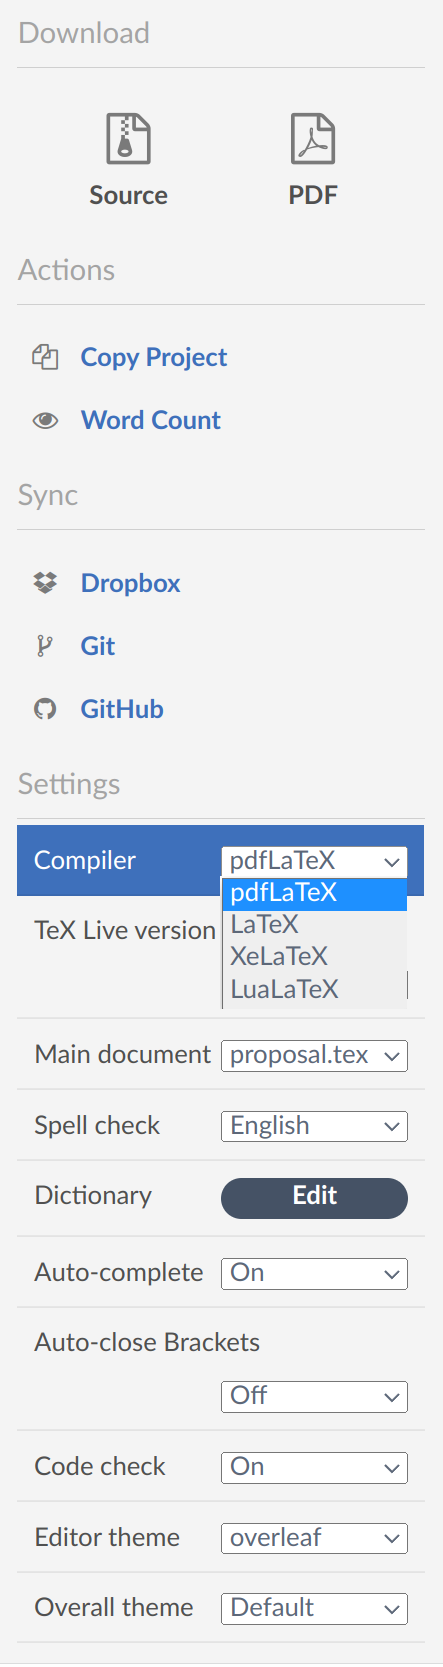
\includegraphics[width=0.40\textwidth]{README_notes/selecting-engine-in-overleaf.png}
  \end{center}
  \caption{Selecting a compiler (\ie TeX engine) in Overleaf}
  \label{fig:selectingTeXEngine}
\end{figure}
\FloatBarrier


\section{Author configuration of the template}
\label{sec:authorConfigs}
The template is designed to handle a thesis written in English or Swedish.
You can set the default language to `english' or `swedish' by passing an option to the documentclass. Note that the language option is written in all lowercase letters; for example, to set the document's language to English:
\begin{lstlisting}[style=latexExampleForAuthors]
\documentclass[english]{kththesis}
\end{lstlisting}

To set the document's language to Swedish (uncomment the following line):
\begin{lstlisting}[style=latexExampleForAuthors]
\documentclass[swedish]{kththesis}
\end{lstlisting}

The language option `swedish' sets the conditional \texttt{\textbackslash ifinswedish} to true.  Among many other things, this conditional is used to configure the KTH cover and the title page to use the chosen language.

The two most common bibliographic engines are supported, \ie BibTeX and BibLaTeX. To set the language to English and use the bibliographic engine to BibTeX you would say:
\begin{lstlisting}[style=latexExampleForAuthors]
\documentclass[english, bibtex]{kththesis}
\end{lstlisting}
To set the language to Swedish and use the bibliographic engine to BibLaTeX you would say:
\begin{lstlisting}[style=latexExampleForAuthors]
\documentclass[swedish, biblatex]{kththesis}
\end{lstlisting}

The above illustrates that you can pass multiple options to the document class separated by commas. Also, note that the options were passed as all lowercase letters.

You can, of course, also modify the formatting of the citations and bibliography. See for example the following code snippet:

\begin{lstlisting}[style=latexExampleForAuthors]
\ifbiblatex
    %\usepackage[language=english,bibstyle=authoryear, citestyle=authoryear, maxbibnames=99]{biblatex}
    %\usepackage[style=numeric,sorting=none,backend=biber]{biblatex}
    \usepackage[bibstyle=authoryear,citestyle=authoryear, maxbibnames=99,language=english]{biblatex}
    % alternatively you might use another style, such as IEEE
    %\usepackage[style=ieee]{biblatex}
    \addbibresource{references.bib}
    %\DeclareLanguageMapping{norsk}{norwegian}
\else
    % The line(s) below are for BibTeX
    \bibliographystyle{bibstyle/myIEEEtran}
    %\bibliographystyle{apalike}
\fi
\end{lstlisting}

To optimize for digital output (this changes the color palette) add the option: \texttt{digitaloutput}. There are also options for A4 or G6 paper: \texttt{a4paper} or \texttt{g5paper} (respectively). The is an option for \texttt{nomenclature}, to produce and refer to equations
\ifnomenclature
as shown in \Cref{ch:NomenclatureExamples}
\fi
.  Finally, there are options for a 1\textsuperscript{st} cycle thesis or 2\textsuperscript{nd} cycle thesis: \texttt{bachelor} and \texttt{master} (respectively); however, these two options are \textbf{not} currently used.

One of the first things that the author(s) will want to do is add the working title and subtitle to the thesis. This is done using the \textbackslash title, \textbackslash subtitle, \textbackslash alttitle, and \textbackslash altsubtitle macros as shown below:
\begin{lstlisting}[style=latexExampleForAuthors]
\title{This is the title in the language of the thesis}
\subtitle{A subtitle in the language of the thesis}

% give the alternative title - i.e., if the thesis is in English,
% then give a Swedish title
\alttitle{Detta är den svenska översättningen av titeln}
\altsubtitle{Detta är den svenska översättningen av undertiteln}
% alternative, if the thesis is in Swedish, then give an English title
%\alttitle{This is the English translation of the title}
%\altsubtitle{This is the English translation of the subtitle}   
\end{lstlisting}

Setting these values once and then using them in many places reduces the work to change them while at the same time ensuring consistency. 

Some additional configuration that the author(s) might do is to set the values of the macros related to the course cycle, course code, date of the thesis, number of credits, degree/exam name, subject area, and if the degree is done external to KTH to set the host information. Consider the snippet below for a student admitted to the ``Bachelor's Programme in Information and Communication Technology (TCOMK)'' program and enrolled in the degree project course ``IA150X Degree Project in Information and Communication Technology, First Cycle 15.0 credits'' and working at a company ``Företaget AB'':
\begin{lstlisting}[style=latexExampleForAuthors]
\hostcompany{Företaget AB} % Remove this line if the project was not done at a host company

\date{\today}

\courseCycle{1}
\courseCode{IA150X}
\courseCredits{15.0}

\programcode{TCOMK}
\degreeName{Bachelors degree}
% Note that the subject area for a Bachelor's thesis (Kandidatexamen)
% should be either Technology or Architecture
% If the thesis is in Swedish, these would be: teknik | arkitektur
% -- Note the use of lower case for the Swedish subject area
\subjectArea{Technology}
\end{lstlisting}

Note that in the above macros you have to give the English or Swedish names in the arguments to \textbackslash degreeName and \textbackslash subjectArea - as shown below:
\begin{lstlisting}[style=latexExampleForAuthors]
\degreeName{Kandidatexamen}
\subjectArea{teknik}
\end{lstlisting}

For a CDATE student enrolled in the course ``DA231X Degree Project in Computer Science and Engineering, Second Cycle 30.0 credits'', the cycle, program, course code, degree, and subject area information would be:
\begin{lstlisting}[style=latexExampleForAuthors]
\programcode{CDATE}
\courseCycle{2}
\courseCode{DA231X}
\courseCredits{30.0}
\degreeName{Degree of Master of Science in Engineering}
\subjectArea{Computer Science and Engineering}
\end{lstlisting}

The set of possible values for the English or Swedish names in the arguments to \textbackslash degreeName are:
\begin{lstlisting}[style=latexExampleForAuthors]
\degreeName{Higher Education Diploma}
\degreeName{Högskoleexamen}

\degreeName{Bachelors degree}
\degreeName{Kandidatexamen}

\degreeName{Master of Architecture}
\degreeName{Arkitektexamen}

\degreeName{Degree of Master of Science in Engineering}
\degreeName{Civilingenjörs}

\degreeName{Magister}
\degreeName{Magisterexamen}

\degreeName{Degree of Master of Science}
\degreeName{Masterexamen}

\degreeName{Master of Science in Engineering and Master of Arts in Education degree}
\degreeName{Civilingenjör och lärare examen}

\degreeName{Degree of Master of Science in Secondary Education}
\degreeName{Ämneslärarexamen}

\degreeName{Both}		# Degree Project in the Field of Technology <teknikområde> and the Main Field of Study <huvudområde>
\degreeName{Same}		# The case when the field of technology <teknikområde> and main field of study <huvudområde> are the same.
\end{lstlisting}

For the last two cases, the code compares the values of subjectArea and secondSubjectArea.

You can find a list of the program codes and school acronyms in the file:\linebreak[4] \texttt{lib/schools\_and\_programs.ins}.

There are a set of rules about what is to be displayed on the KTH cover. These can be found at \url{https://www.kth.se/social/group/sprakkommitten/page/omrade-for-examensarbete/}.

One of the reasons for many of the macros shown above and below is to collect the information that is needed to report the approved thesis in Digitala Vetenskapliga Arkivet (DiVA) and to report the title(s) and grade in \foreignlanguage{swedish}{Lokalt adb–baserat dokumentationssystem (LADOK)}.

National subject categories are a \textbf{required} field in the DiVA record. These categories follow a definition by \foreignlanguage{swedish}{SCB} (nowadays known as \foreignlanguage{swedish}{Statistikmyndigheten} or in English: Statistics Sweden) and HSV (\foreignlanguage{swedish}{Högskoleverket} - nowadays known as  \foreignlanguage{swedish}{Universitetskanslersämbetet (UK-ämbetet)} and \foreignlanguage{swedish}{Universitets- och högskolerådet (UHR)} or in English: Swedish Higher Education Authority and Swedish Council for Higher Education).
While these codes refer to research areas, these codes are also used in KTH to indicate the area of the thesis. The guidance that I received from the Linköping University library was that one should try to use 5-digit codes when possible. Some examples of these codes are shown in Table~\ref{tab:nationalsubject categories}.
\begin{description}[leftmargin=!, labelwidth =\widthof{\texttt{\textbackslash nationalsubjectcategories\{\}}}]
\item [\texttt{\textbackslash nationalsubjectcategories\{\}}] comma separated list of national subject category codes - each a 3 or 5 digit code
\end{description}

\Needspace*{2\baselineskip}
An example for a thesis in Computer Science and Computer Systems:
\begin{lstlisting}[style=latexExampleForAuthors]
\nationalsubjectcategories{10201, 10206}
\end{lstlisting}

You can find the subjects and their codes in:\\ \url{https://www.scb.se/contentassets/3a12f556522d4bdc887c4838a37c7ec7/standard-for-svensk-indelning--av-forskningsamnen-2011-uppdaterad-aug-2016.pdf}\\
and\\
\url{https://www.scb.se/contentassets/10054f2ef27c437884e8cde0d38b9cc4/oversattningsnyckel-forskningsamnen.pdf}

\begin{table}[!ht]
  \begin{center}
    \caption{Examples of some national subject categories and their codes}
    \label{tab:nationalsubject categories}
    \begin{tabular}{p{0.85cm} L{6.2cm} L{6.2cm}} % <-- Alignments: 1st column left, 2nd middle, with vertical lines in between
      \textbf{Code}  & \textbf{Category (in Swedish)} & \textbf{Category (in English)} \\
      \hline
102 & \foreignlanguage{swedish}{Data- och informationsvetenskap (Datateknik)} &   Computer and Information Sciences \\
      \hline
10201 & \foreignlanguage{swedish}{Datavetenskap (datalogi)} & Computer Sciences \\
      \hline
10202 & \foreignlanguage{swedish}{Systemvetenskap, informationssystem och informatik} (\foreignlanguage{swedish}{samhällsvetenskaplig inriktning} under 50804) &
Information Systems (Social aspects to be 50804)\\
      \hline
10203 & \foreignlanguage{swedish}{Bioinformatik (beräkningsbiologi)} (\foreignlanguage{swedish}{tillämpningar} under 10610) & Bioinformatics (Computational Biology) (applications to be 10610) \\
      \hline
10204 & \foreignlanguage{swedish}{Människa-datorinteraktion (interaktionsdesign)} (\foreignlanguage{swedish}{Samhällsvetenskapliga aspekter} under 50803) & Human Computer Interaction (Social aspects to be 50803)\\
      \hline
10205 & \foreignlanguage{swedish}{Programvaruteknik} & Software Engineering \\
      \hline
10206 & \foreignlanguage{swedish}{Datorteknik} & Computer Engineering \\
      \hline
10207 & \foreignlanguage{swedish}{Datorseende och robotik (autonoma system) }& Computer Vision and Robotics (Autonomous Systems) \\
      \hline
10208 & \foreignlanguage{swedish}{Språkteknologi (språkvetenskaplig databehandling)} & Language Technology (Computational Linguistics) \\
      \hline
10209 & \foreignlanguage{swedish}{Medieteknik} & Media and Communication Technology \\
      \hline
10299 & \foreignlanguage{swedish}{Annan data- och informationsvetenskap} & Other Computer and Information Science \\
      \hline
      \hline
202   & \foreignlanguage{swedish}{Elektroteknik och elektronik} & Electrical Engineering, Electronic Engineering, Information Engineering \\
      \hline
20201 & \foreignlanguage{swedish}{Robotteknik och automation} & Robotics \\
      \hline
20202 & \foreignlanguage{swedish}{Reglerteknik} & Control Engineering \\
      \hline
20203 & \foreignlanguage{swedish}{Kommunikationssystem} & Communication Systems \\
      \hline
20204 & \foreignlanguage{swedish}{Telekommunikation} & Telecommunications \\
      \hline
20205 & \foreignlanguage{swedish}{Signalbehandling} & Signal Processing \\
      \hline
20206 & \foreignlanguage{swedish}{Datorsystem} & Computer Systems \\
      \hline
20207 & \foreignlanguage{swedish}{Inbäddad systemteknik} & Embedded Systems \\
      \hline
20299 & \foreignlanguage{swedish}{Annan elektroteknik och elektronik} & Other Electrical Engineering, Electronic Engineering, Information Engineering \\
      \hline
    \end{tabular}
  \end{center}
\end{table}



\FloatBarrier



\section{Author macros}
\label{sec:authorMacros}
It is assumed that there can only be 1 or 2 authors. For many years now 2\textsuperscript{nd} cycle theses are expected to only have one author.

For the author or first author, there are a number of macros defined to store information about the author, so that it can later be used in multiple places -- for example, the KTH cover (produced with \texttt{\textbackslash kthcover)}, the title page (produced with \texttt{\textbackslash titlepage}, the ``For DIVA'' section at the end of the thesis (produced with \linebreak[4]
\texttt{\textbackslash divainfo\{pg:lastPageofPreface\}\{pg:lastPageofMainmatter\}}), and possibly a JavaScript Object Notation (JSON) file named \texttt{fordiva.json} produced as a by product of the \texttt{\textbackslash divainfo}. Note that the actual section name has DiVA set in all caps - which hopefully should not occur in the thesis! If the string DiVA set in all caps, does have to appear, then the section heading should be preceded by four euro signs and followed by four more euro signs (as is done this doucment).

The author-related macros are:
\begin{description}[leftmargin=!, labelwidth =\widthof{\texttt{\textbackslash secondAuthorsFirstname\{\}}}]
\item [\texttt{\textbackslash authorsLastname\{\}}] the last name of the author\footnote{Note that the author's name can include a suffix such as ``, Jr.'' or `` Jr.'', i.e., the suffix can be separated with a comma or not -- as the author prefers to write their name.}

\item [\texttt{\textbackslash authorsFirstname\{\}}] the first name of the author

\item [\texttt{\textbackslash email\{\}}] the KTH e-mail address of the author

\item [\texttt{\textbackslash kthid\{\}}] the author's kthid, this generally starts with the string ·``u1'' and is a unique identifier for every KTH user.

% As per email from KTH Biblioteket on 2021-06-28 students cannot have an OrCiD reported for their degree project
\item [\texttt{\textbackslash authorsSchool\{\}}] the value is generally of the form:\linebreak[4] \texttt{\textbackslash schoolAcronym\{EECS\}}. The currently supported school acronyms are: ABE, CBH, EECS, ITM, and SCI. These are defined in the file\linebreak[4] \texttt{schools\_and\_programs.ins}.
\end{description}

If the first author is not in Stockholm, Sweden when the acknowledgements are written, then add that information via the macros described below.
This information will be used when generating the acknowledgements signature. The acknowledgements signature is the text at the end of the acknowledgements and it gives the place where the author(s) is/are when writing the acknowledgements and also gives the date and name(s).
\begin{description}[leftmargin=!, labelwidth =\widthof{\texttt{\textbackslash secondAuthorsFirstname\{\}}}]
\item [\texttt{\textbackslash authorCity\{A City\}}] specify the city

\item [\texttt{\textbackslash authorCountry\{A Country\}}] specify the country

\item [\texttt{\textbackslash authorCityCountryDate\{\}}] pass into this function the month and year for the acknowledgement. This can be a string such as January 2022 or it can be a \LaTeX\  expression, such as \textbackslash MONTH\textbackslash enspace\textbackslash the\textbackslash year.
\end{description}

If there is a second author and the place, month, and year are \textbf{all} the same, then specify the month and year for only the \textbf{first} author:
\begin{lstlisting}[style=latexExampleForAuthors]
\authorCityCountryDate{\MONTH\enspace\the\year}
\end{lstlisting}

If there is a second author and the place is different, then say:
\begin{lstlisting}[style=latexExampleForAuthors]
\authorCityCountryDate{}
\end{lstlisting}
\clearpage

If there is a second author, the macros are:
\begin{description}[leftmargin=!, labelwidth =\widthof{\texttt{\textbackslash secondAuthorsFirstname\{\}}}]
\item [\texttt{\textbackslash secondAuthorsLastname\{\}}] the last name of the 2\textsuperscript{nd} author
\item [\texttt{\textbackslash secondAuthorsFirstname\{\}}] the first name of the 2\textsuperscript{nd} author
\item [\texttt{\textbackslash secondemail\{\}}] the KTH e-mail address of the 2\textsuperscript{nd} author
\item [\texttt{\textbackslash secondkthid\{\}}] the 2\textsuperscript{nd} author's kthid
% As per email from KTH Biblioteket on 2021-06-28 students cannot have an OrCiD reported for their degree project
\item [\texttt{\textbackslash secondAuthorsSchool\{\}}] the school of the 2\textsuperscript{nd} author
\end{description}

If the second author is not in the same place as the first author, then add the relevant information using the macros below.  This information will be used when generating the acknowledgements signature.
\begin{description}[leftmargin=!, labelwidth =\widthof{\texttt{\textbackslash secondAuthorsFirstname\{\}}}]
\item [\texttt{\textbackslash secondAuthorCity\{A City\}}]  specify the city

\item [\texttt{\textbackslash secondAuthorCountry\{A Country\}}] specify the country

\item [\texttt{\textbackslash secondAuthorCityCountryDate\{\textbackslash MONTH\textbackslash enspace\textbackslash the\textbackslash year\}}]  pass into this function the month and year for the acknowledgement
\end{description}

If the second author is the same place as the first author, then comment out or delete the \textbackslash secondAuthorCityCountryDate\{\} as shown below:
\begin{lstlisting}[style=latexExampleForAuthors]
%\secondAuthorCityCountryDate{}
\end{lstlisting}

\section{Starting to write}
\label{sec:startingToWrite}

As you write you will notice "todo" notes in the template. They follow the following conventions:
\begin{lstlisting}[style=latexExampleForAuthors]
\generalExpl{Comments/directions/... in English}
\sweExpl{Text på svenska}
\engExpl{English descriptions about formatting}
\sweExpl{warnings}
\end{lstlisting}


\subsection{Working abstract}
\label{sec:wrtingFirstAbstract}
I generally recommend that every student start by writing a working abstract, this will help you keep your focus. To find where you can start to enter your abstract look in the \textit{examplethesis.tex} file for the line:
\begin{lstlisting}[style=latexExampleForAuthors]
\generalExpl{Enter your abstract here!}
\end{lstlisting}

There is lots of information already in the template to help you with entering text, equations, \etc in your abstract. \textbf{NB} Abstracts are supposed to stand by themselves, this means no footnotes, no cross-references, no figures, no tables, \etc.

I suggest avoiding the use of the defined acronyms in abstracts \ie spell them out rather than using the glossary commands. This is due to the fact that the \texttt{glossaries} package (that is being used to support acronyms) does not directly provide support for multiple languages and because I do not understand how to programmatically create plurals of acronyms in Swedish or other languages. Even in an English abstract, it is desirable to avoid using the glossary commands - as this makes subsequent processing of the abstracts harder - since one has to make sure that the list of acronyms and their definitions are provided to any program that will process this \LaTeX\  source code. For this reason, later versions of this template include the acronyms.tex file after the metadata for DiVA.

\subsection{Structure of the abstracts and summaries}
The basic \LaTeX\  structure for an abstract or summary is shown below (for the case of an English abstract and a Swedish summary \ie sammanfattning):
\begin{lstlisting}[style=latexExampleForAuthors]
\begin{abstract}
  \markboth{\abstractname}{}
\begin{scontents}[store-env=lang]
eng
\end{scontents}

\begin{scontents}[store-env=abstracts,print-env=true]
here is where you abstract goes.
\end{scontents}

\subsection*{Keywords}
\begin{scontents}[store-env=keywords,print-env=true]
% If you set the EnglishKeywords earlier, you can retrieve them with:
\InsertKeywords{english}
% If you did not set the EnglishKeywords earlier then simply enter the comma separate keywords here:
%such as: Canvas Learning Management System, Docker containers, Performance tuning
\end{scontents}
\end{abstract}

\cleardoublepage
\babelpolyLangStart{swedish}
\begin{abstract}
    \markboth{\abstractname}{}
\begin{scontents}[store-env=lang]
swe
\end{scontents}
\begin{scontents}[store-env=abstracts,print-env=true]
Swedish summary goes here
\end{scontents}
\subsection*{Nyckelord}
\begin{scontents}[store-env=keywords,print-env=true]
% SwedishKeywords were set earlier, hence we can use alternative 2
\InsertKeywords{swedish}
\end{scontents}
\end{abstract}
\babelpolyLangStop{swedish}
\end{lstlisting}

It is important to note that the contents of the \texttt{scontents} environment for the abstracts are stored \textbf{verbatim}, \ie the \LaTeX\  is \textbf{not} executed. The reason for this is to be able to later have a program that can manipulate the source \LaTeX\  to convert it to HTML for use in announcements, calendar events, and for DiVA. This means that if you write the following:
\begin{lstlisting}[style=latexExampleForAuthors]
\begin{scontents}[store-env=abstracts,print-env=true]
\input{abstract.txt}
\end{scontents}
\end{lstlisting}
\noindent what will end up in your abstract in the metadata save for DiVA will simply be: \texttt{''\textbackslash input{abstract.tex}''} -- which means that someone will have to cut and paste your actual abstract to insert it into DiVA.

It is also important to that that the following lines:
\begin{lstlisting}[style=latexExampleForAuthors]
\begin{scontents}[store-env=lang]
eng
\end{scontents}
\end{lstlisting}
\noindent \textbf{must} to be before the \texttt{scontents} environment for the abstracts and keywords -- as these lines indicate what language the subsequent abstract and keywords are in. The three-character code used for the language is the ISO 639-2 Code – specifically the "B" (bibliographic) variant of these codes --- as these codes are used in the DiVA metadata to tag what language is used.

\subsection{Acronyms}
\label{sec:addingAcronyms}
You may want to define an acronym to help you with your writing, as this can both reduce the amount of typing and help your reader by providing consistent use of acronyms. The acronyms' definitions can be found in the file \textit{lib/acronyms.tex}. The file contains some examples. I generally try to sort the lines to help find which acronyms I already have defined and keep track of the new one(s) I want to add.

\subsection{Some predefined macros to help when writing}
\label{sec:predefine}

The file \textit{lib/defines.tex} includes some macros that will help you when writing. This includes \textbackslash etc, to give you ``\etc'', \textbackslash eg, \textbackslash ie, and \textbackslash etal.
The file also defines \textbackslash first, \textbackslash Second, ... \textbackslash eighth to give you \first, \Second, \third, ... \eighth. Note that `Second' is written with an initial capital letter to avoid conflict with the unit `second' in the \texttt{siunitx} package.

\subsection{Additional abstract(s)}
\label{sec:additionalAbstracts}

All theses at KTH are \textbf{required} to have an abstract in both \textit{English} and \textit{Swedish}. However, in addition to this, many students want to add abstracts in additional languages. The template comes pre-configured with places for abstracts in several other languages. If there is a language that you want to use that is not already supported, there are directions for how to add an additional language. If there are abstracts in languages that you do not want, please delete them or comment them out (see \Cref{sec:hideComment}).

\subsection{Removing and hiding parts that you do not want}
\label{sec:hideComment}

It is quite likely that you will find parts of the template that you do not want/need. One way of dealing with this is to delete them, and another way is to comment them out. Personally, I like to comment things out, in case I actually do want to be able to read it in the \LaTeX\  file or uncomment it later. To comment out a portion of the file, simply use the following environment:

\begin{lstlisting}[style=latexExampleForAuthors]
\begin{comment}
    **** what you want to comment out ****
\end{comment}
\end{lstlisting}

For example, if you are not interested in the Swedish language \texttt{todo} notes, you can look for lines with ``\textbackslash sweExpl'' in them and comment them out (or delete them).

\subsection{Removing the README\_notes}
At some point you will no longer want this README information. You can remove it by removing the line
\textbackslash include\{README\_notes/README\_notes\} -- from the \textit{examplethesis.tex} file. You can then remove the \textbf{README\_notes} directory.

Unless you are an examiner or an administrator you can delete the file: \texttt{README\_notes/README\_examiner\_notes.tex} and delete the include of this file from near the end of the template (\ie \textit{examplethesis.tex}. You can also delete the directory \textbf{README\_notes/README\_examiner-figures}.


\section[Copyright or Creative Commons License]{Copyright or Creative Commons\\ License}
\label{sec:copyrightOrCClicense}
It is possible to have several variants of the bookinfo page\footnote{When printed double sided, the bookinfo page is the back of the title page.}:
\begin{enumerate}[labelwidth =\widthof{\textbf{Creative Commons (CC)}}, leftmargin = !]
    \item[copyright] If you want to have a bookinfo page, include the line saying \textbackslash bookinfopage.
    \item[Creative Commons (CC)] If you want to have a bookinfo page but want to have a Creative Commons license, then include \textbackslash bookinfopage and use and configure the \texttt{doclicense} package as described below.
    \item[none] If you do \textbf{not} want to have a bookinfo page, comment the line saying \textbackslash bookinfopage and add a \textbackslash cleardoublepage.
\end{enumerate}

For background about Creative Commons licenses, see:
\url{https://www.kb.se/samverkan-och-utveckling/oppen-tillgang-och-bibsamkonsortiet/open-access-and-bibsam-consortium/open-access/creative-commons-faq-for-researchers.html} and \url{https://kib.ki.se/en/publish-analyse/publish-your-article-open-access/open-licence-your-publication-cc}.

Note that the lowercase version of the Creative Commons license has to be used in the modifier, \ie one of: by, by-nc, by-nd, by-nc-nd, by-sa, by-nc-sa, or zero. For the list of supported licenses, see the documentation for the \texttt{doclicense} package.

Note that if the \texttt{doclicense} package is used, it automatically redefines \texttt{\textbackslash bookinfopage} to be \texttt{\textbackslash bookinfopageCC}.

\subsection{Example configuration to have a CC BY-NC-ND license}

\begin{lstlisting}[style=latexExampleForAuthors]
\usepackage[
    type={CC},
    modifier={by-nc-nd},
    version={4.0},
    hyphenation={RaggedRight},
]{doclicense}
\end{lstlisting}

Note that the option ``hyphenation={RaggedRight}'' can be used with the configuration of the package to set the license information with a ragged right margin rather that as a filled and justified paragraph.


\subsection{Example configuration to have a CC BY-NC-ND license with a Euro symbol rather than a Dollar sign}

\begin{lstlisting}[style=latexExampleForAuthors]
\usepackage[
    type={CC},
    modifier={by-nc-nd},
    version={4.0},
    imagemodifier={-eu-88x31},  % to get Euro symbol rather than Dollar sign
    hyphenation={RaggedRight},
]{doclicense}
\end{lstlisting}


\subsection{Example configuration to have a CC0 license}

\begin{lstlisting}[style=latexExampleForAuthors]
\usepackage[
    type={CC},
    modifier={zero},
    version={1.0},
]{doclicense}
\end{lstlisting}

\section{Use of fonts within the thesis}
\label{sec:useOfFontsWithinThesis}

The choice of fonts is a very individual matter and may be affected by the kind of content that you are trying to write, the language that you are writing in, and what you want to convey to your reader. However, some points to keep in mind are:
\begin{itemize}
    \item Use fonts with serifs for the body of your thesis, their presence makes it much easier for your reader.

    \item Use sans serif fonts for headings. This helps your reader distinguish them from the body.

    \item Be very careful when using fonts that are not widely available\footnote{For example, even though it is widely used. not everyone has the Arial font.}. Unless you embed the fonts that you have used, your reader may not see what you want them to see. Ideally, you should embed all fonts -- even if you only embed the subset you use.

    \item Although there are fonts that have a huge number of characters in them, they might not have the characters that you need.

    \item There are also fonts that, although they have a vast number of characters in them, do not have the math table that \LaTeX\ needs to be able to set mathematical content\footnote{An example of such a font is Google's Noto font. Even though it includes a vast number of characters, it lacks a math table -- although there is an awareness of this missing feature}.
\end{itemize}

What can you do when the fonts you use are missing characters that you need to use? One solution is to use a font that has the character(s) that you want and then make use of them in the places that you need to.

\warningExpl{The details of working with different fonts and characters is a rather complex area and not for the faint-hearted. However, if you \textbf{really} want to have specific characters, \XeLaTeX\ and \LuaLaTeX\ have the means to help you realize what you want. }


\end{document}

% \subfile{README_author}

% \cleardoublepage
% information about the template for everyone
% % \newacronym[⟨options⟩]{⟨label⟩}{⟨abbrv⟩}{⟨long⟩}
%\newglossaryentry{⟨label⟩}{type=\acronymtype,
%name={⟨abbrv⟩},
%description={⟨long⟩},
%text={⟨abbrv⟩},
%first={⟨long⟩ (⟨abbrv⟩)},
%plural={⟨abbrv⟩s},
%firstplural={⟨long⟩s (⟨abbrv⟩s)},
%⟨options⟩}

%\newacronym{API}{API}{Application Programming Interface}
\newglossaryentry{tld:API}{type=readme,
name={API},
description={Application Programming Interface},
text={API},
first={Application Programming Interface (API)},
plural={APIs},
firstplural={Application Programming Interfaces (APIs)},
}
\newglossaryentry{tld:DiVA}{type=readme, name={DiVA}, description={Digitala Vetenskapliga Arkivet},
first={Digitala Vetenskapliga Arkivet (DiVA)}}
\newglossaryentry{tld:IMRAD}{type=readme, name={IMRAD}, description={Introduction, Methods, Results, and Discussion},
first={Introduction, Methods, Results, and Discussion (IMRAD)}}
\newglossaryentry{tld:JSON}{type=readme, name={JSON}, description={JavaScript Object Notation},
first={JavaScript Object Notation (JSON)}}
\newglossaryentry{tld:KOPPS}{type=readme, name={KOPPS}, description={Kurs- och programplaneringssystemet},
first={Kurs- och programplaneringssystemet (KOPPS)}}
\newglossaryentry{tld:KTH}{type=readme, name={KTH}, description={KTH Royal Institute of Technology},
first={KTH Royal Institute of Technology (KTH)}}
\newglossaryentry{tld:LADOK}{type=readme, name={LADOK}, description={Lokalt adb–baserat dokumentationssystem},
first={Lokalt adb–baserat dokumentationssystem (LADOK)}}
\newglossaryentry{tld:TIMTM}{type=readme, name={TIMTM}, description={Interactive Media Technology}
first={Interactive Media Technology (TIMTM)}}
\newglossaryentry{tld:TMMTM}{type=readme, name={TMMTM}, description={Media Management}
first={Media Management (TMMTM)}}


\lstdefinestyle{latexExample}{
language=[LaTeX]{TeX},
    breaklines=true,
    postbreak=\mbox{\textcolor{red}{$\hookrightarrow$}\space},
    basicstyle=\small\tt,
    keywordstyle=\color{blue}\sf,
    identifierstyle=\color{magenta},
    commentstyle=\color{cyan},
    backgroundcolor=\color{yellow!15},
    tabsize=2,
    columns=flexible,
}
\lstset{style=latexExample}
\newcommand{\dname}[1]{\textbf{#1}}
\newcommand{\fname}[1]{\texttt{#1}}
\chapter{README and notes about the template}
\label{ch:READMEnotes}

\glsresetall[readme]
This document, written by Gerald Q. Maguire Jr,  describes the thesis template that I have developed for use at \gls{tld:KTH} and provides some background about why it is the way that it is. It is important to note that the template is \textbf{not prescriptive}, as not every thesis will have all of the parts that the template shows. However, if there is something that you decide to leave out, you should make a conscious decision to do so and you should consider the impact this may have on your thesis being approved by the examiner.

Fundamental to the design of the template are several key factors:
\begin{itemize}
    \item Helping students be successful in their degree project,
    \item Helping students produce a high-quality thesis, and
    \item Supporting all of the (relevant) phases of the degree project process.
\end{itemize}

There are several thousand theses written each year by \gls{tld:KTH} students. Every approved thesis will be entered into \gls{tld:DiVA} (independent of whether the full text is made available via \gls{tld:DiVA}). Collecting the data necessary for \gls{tld:DiVA} was a major driving force in the design of the template. This data is useful for many of the phases of the degree project, such as announcing the oral presentation.
    
This template is \textbf{not} designed for use by \gls{tld:TIMTM} and \gls{tld:TMMTM} students - as students in these two programmes are using a different structure for their reports (there is another template available for them).

\textbf{This document is a work in progress.}

\section{Introduction}
This template evolved (radically) from an earlier thesis template that was widely used at \gls{tld:KTH}. The direction of this evolution was based on the DOCX template that was developed over many years for use with students for whom I was the examiner and/or supervisor. The suggested structure and contents of the thesis reflect my experience as an examiner for more than 590 degree projects and the experience I have had as a teacher and examiner for the course II2202 Research Methodology and Scientific Writing. The template also reflects my interest as a member of KTH's Language Committee in facilitating the parallel use of English and Swedish at \gls{tld:KTH}, as well as supporting other languages. The latter aspect
reflects my experience with double-degree students, who often need to have at least the abstract of their thesis available in the language(s) of their home university. The thesis template also reflects
my experience in entering the metadata for hundreds of theses into \gls{tld:DiVA} and announcing a very large number of degree project seminars.

\Cref{sec:expectedUsers} describes several different groups of users and how the template is relevant to them.

There were several major thoughts influencing the design of this template:
\begin{enumerate}[leftmargin=*, label=\textbf{Thought \arabic*}, ref={Thought \arabic*}]
    \item \label{thought:helpStudent} The template should help a student be successful in their degree project and help them produce a high-quality thesis in conjunction with their degree project.
    
    \item \label{thought:process} The template should help support all of the (relevant) phases of the degree project process.
    
    \item \label{thought:reducingDataEntry} Redundant data entry should be minimized in order to increase consistency.
    
    \item \label{thought:volume} There are several thousand theses written each year at \gls{tld:KTH}. In fact, theses are the second most common type of publication at \gls{tld:KTH}.
    
    \item \label{thought:inDiVA} Every approved thesis will have at least its metadata entered into \gls{tld:DiVA}. \gls{tld:DiVA} features multi-language support for title, subtitle, abstract, and keywords.
\end{enumerate}

\section{Deliminations}

This template is \textbf{not} designed for use by \gls{tld:TIMTM} and Media Management \gls{tld:TMMTM} students - as students in these two programmes are using a different structure for their reports (there is another template available for them).

Additionally, I have been told by one of my colleagues in applied mathematics that theses in this area generally do not follow the \gls{tld:IMRAD} structure.

Some parts of the template are conditional based on the value of a switch: \texttt{\textbackslash ifinswedish}. The idea is to easily have a single template that supports theses written in English or Swedish. However, in many places, the conditional has not been used but could be. Examples of this include the Swedish names for chapters and sections. Generally this information is in a note after the English chapter or section name. More complete implementation of the use of this condition remains as future work.

The template does not fully support the G5 paper format. In particular, the \gls{tld:KTH} cover (produced with \texttt{\textbackslash kthcover)} and back cover (produced with \texttt{\textbackslash kthbackcover)}) have only been adapted for A4 paper. Support for G5 paper remains as future work.

The handling of the subject area (Swedish: \foreignlanguage{swedish}{Område för examensarbete}) is currently incomplete and remains as future work. Personally, I'm still struggling to understand the rules and how one knows what the correct values are (especially for cases of \first dual degrees and \Second combinations of technical subjects and education degrees).

\section{Structure of the files for the template}
\Cref{tab:file_structure} shows the structure of the files for the template. These files are generally taken either from an existing Overleaf project, a ZIP file, or a github.

One hope is that by automatically extracting information from various sources, this information is more likely to be \textit{correct} and \textit{consistent} (supporting \ref{thought:reducingDataEntry}). This approach has been used to generate two of the files used for the template. These files are:
\begin{enumerate}
    \item The file \fname{custom\_configuration.tex} contains macros and values for configuring a project. These values are generally expected to be known at the start of the project, \eg author(s), supervisor(s). examiner, course code for the degree project program code, \etc. While this file can be manually edited, it was designed to be generated by a program that I have written that extracts most of the data from the Canvas course being used in conjunction with the degree project. One of the goals of using such a program is to automatically extract data from Canvas, the \gls{tld:KTH} profile \gls{tld:API}, \gls{tld:KOPPS}, and other sources. The macros for defining this information are described in Sections \ref{sec:authorMacros}, \ref{sec:supervisorMacros}, and \ref{sec:examinerMacros} - for authors, supervisors, and examiner (respectively).

    \item The file \texttt{schools\_and\_programs.ins} contains the English and Swedish names of schools and programs. This information was extracted by a program from \gls{tld:KOPPS}.
\end{enumerate}

We will assume that these files have been generated by someone. Later we will examine who this someone might be for each of these files.

\begin{table}[!ht]
    \caption{Structure of files for the template}
    \label{tab:file_structure}
\resizebox{\columnwidth}{!}{%
    \begin{tabular}{l l p{4cm}<{\raggedright}}
%\textbf{Top level} & \textbf{2\textsuperscript{nd} level} & \textbf{Description} \\
\hline
\dname{bibstyle} & \multicolumn{2}{c}{\textbf{directory containing files related to the style of the bibliography}} \\
{} & \fname{myIEEEtran.bst} & a bibtex style file  \\
\hline
\dname{figures} & \multicolumn{2}{c}{\textbf{directory containing files for figures}} \\
\hline
\dname{lib} & \multicolumn{2}{c}{\textbf{directory containing various library files}}  \\
& \fname{acronyms.tex} & a place to define the acronyms that will or might be used \\
& \fname{defines.tex} & some generally useful defines \\
& \fname{includes-after-hyperref.tex} & a special include file for packages that have to be included \textbf{after} the hyperref package \\
& \fname{includes.tex} & a centralized place to include packages that might be useful \\
& \fname{kthcolors.tex} & defines a number of colors from the \gls{tld:KTH} palette \\
& \fname{pdf\_related\_includes.tex} & includes to be able to add the title and other information to the PDF file \\
& \fname{schools\_and\_programs.ins} & English and Swedish names of schools and the programs \\
\hline
\fname{custom\_configuration.tex} & & macros and values for configuring a project\\
\fname{examplethesis.tex} & & an example of the thesis itself \\
\fname{kth\_logo.png} & & the \gls{tld:KTH} logo for use on the cover \\
\fname{KTH\_ROYAL\_INSTITUTE\_OF\_TECHNOLOGY\_logotype.png} & & \gls{tld:KTH} logotype for use on the English language cover \\
\fname{kththesis.cls} & & the kththesis class file \\
\fname{README\_notes.tex} & & these notes \\
\fname{references.bib} & & references that may be cited in the thesis \\
\end{tabular}
}  % End of resizebox

\end{table}
%\FloatBarrier
\clearpage


\section{Expected users and their differences}
\label{sec:expectedUsers}
This template is relevant to several different sets of users:
\begin{enumerate}[leftmargin=*,label=\textbf{Users \arabic*}, ref={Users \arabic*}]
    \item \label{users:authors} Author or Authors (see \Cref{sec:authors}),
    \item \label{users:others} Those working together with the author(s) during the degree project process (see \Cref{sec:examinerAdvisorsOpponent}),
    \item \label{users:admins} Administrative staff working with the document after it has been approved by the examiner (see \Cref{sec:adminStaff}), and
    \item \label{users:readers} The (hopefully) many (human) readers of the final document (see \Cref{sec:readers}).
    \item \label{users:searchEngines} The (hopefully) many computers reading the metadata and the full text of the final document (see \Cref{sec:searchEngines}).
    \item \label{users:maintainer} Those who are maintaining or updating this template (see \Cref{sec:maintainer}).
\end{enumerate}

Each of these different sets of users has different needs and perspectives. The following subsections describe these needs and perspectives.

For information for authors see \Cref{{ch:READMEauthor}} - located in the file \texttt{README\_author.tex}.

\section{Those working in parallel with the authors(s) during the degree project}
\label{sec:examinerAdvisorsOpponent}
Those working together with the author(s) during the degree project process include the examiner, supervisor(s), and the opponent(s).

\subsection{Supervisor}
\label{sec:supervisorMacros}
If a degree project is done in industry, there is generally an industrial supervisor in addition to the academic supervisor(s). The template supports up to 3 supervisors (typically an academic supervisor, an industrial supervisor, and sometimes an additional academic or industrial supervisor). The choice of up to three reflects my experience and observation of prior theses in \gls{tld:DiVA}. Note that there is expected to be at least one supervisor. The supervisors are enumerated as A, B, and C. For each of A, B, and C as appropriate, replace the "X" in the following macros:
\begin{description}[leftmargin=!, labelwidth =\widthof{\texttt{\textbackslash secondAuthorsFirstname\{\}}}]
\item [\texttt{\textbackslash supervisorXsLastname\{\}}] the last name of the supervisor
\item [\texttt{\textbackslash supervisorXsFirstname\{\}}] the first name of the supervisor
\item [\texttt{\textbackslash supervisorXsEmail\{\}}] e-mail address of the supervisor
\end{description}

If the supervisor is from within \gls{tld:KTH}, then add their KTHID, School, and Department info:
\begin{description}[leftmargin=!, labelwidth =\widthof{\texttt{\textbackslash secondAuthorsFirstname\{\}}}]
\item [\texttt{\textbackslash supervisorXsKTHID\{\}}] the supervisor's kthid 
\item [\texttt{\textbackslash supervisorXsSchool\{\}}] the school of the supervisor
\item [\texttt{\textbackslash supervisorXsDepartment\{\}}] the department of the supervisor
\end{description}

If the supervisor is from outside of \gls{tld:KTH}, then add their organization with:
\begin{description}[leftmargin=!, labelwidth =\widthof{\texttt{\textbackslash secondAuthorsFirstname\{\}}}]
\item [\texttt{\textbackslash supervisorXsOrganization\{\}}] the supervisor's organization
\end{description}

\subsection{Examiner}
\label{sec:examinerMacros}
I assume that there is only a single examiner for a given thesis\footnote{Statistically, there are very few theses with multiple examiners, and this generally occurs for students either in a double degree program or when there are two students in a 1\textsuperscript{st} cycle degree project from different schools, then there might be one examiner for each student. As the case of more than one examiner occurs very infrequently, I have left it for future work. The pseudo-JSON structure is set up to handle multiple examiners, but additional macros would be needed in a similar fashion as used for multiple supervisors, and this metadata would have to be conditionally added where appropriate.}. For this examiner, the relevant macros are:
\begin{description}[leftmargin=!, labelwidth =\widthof{\texttt{\textbackslash secondAuthorsFirstname\{\}}}]
\item [\texttt{\textbackslash examinersLastname\{\}}] the last name of the examiner
\item [\texttt{\textbackslash examinersFirstname\{\}}] the first name of the examiner
\item [\texttt{\textbackslash examinersEmail\{\}}] e-mail address of the examiner
\end{description}

If the examiner is from within \gls{tld:KTH}, then add their KTHID, School, and Department info:
\begin{description}[leftmargin=!, labelwidth =\widthof{\texttt{\textbackslash secondAuthorsFirstname\{\}}}]
\item [\texttt{\textbackslash examinersKTHID\{\}}] the examiner's kthid 
\item [\texttt{\textbackslash examinersSchool\{\}}] the school of the examiner
\item [\texttt{\textbackslash examinersDepartment\{\}}] the department of the examiner
\end{description}

If the examiner is from outside of \gls{tld:KTH}, then add their organization with:
\begin{description}[leftmargin=!, labelwidth =\widthof{\texttt{\textbackslash secondAuthorsFirstname\{\}}}]
\item [\texttt{\textbackslash examinersOrganization\{\}}] the examiner's organization
\end{description}


I assume that someone (such as the examiner) will generate the file:\linebreak[4] \fname{custom\_configuration.tex}. This assumption is based upon the fact that the examiner knows who the student or students are who will be working on a given degree project, who the supervisor or supervisors are, what program the student is in, course code, \ldots . Ideally, this file should be generated automatically by some computer program so that each student or pair of students in a group gets a customized template automatically via the Canvas course. However, currently, the file is generated using a command line program (\texttt{create\_customized\_JSON\_file.py}) to generate a \gls{tld:JSON} file. Subsequently, a separate program (\texttt{customize\_LaTeX\_project.py}) takes this \gls{tld:JSON} data and creates the appropriate \LaTeX\ commands and inserts this information into the file and then inserts this file into a ZIP file, either replacing or augmenting the \fname{custom\_configuration.tex} within this ZIP file (if one exists). There is an option for this second program \texttt{--initialize} that causes the program to simply replace the file rather than appending the new information to the end of the file.

The above programs are available from \url{https://github.com/gqmaguirejr/E-learning}. The README file for this github contains information about how to run the programs, their options, and gives examples.

\subsection{Opponent(s) and oral presentation}
\label{sec:opponentMacros}
Unlike the supervisors and examiner, the macros related to the opponent and oral presentation are in the \fname{examplethesis.tex} file.
The macro for the opponent(s) is: 
\begin{description}[leftmargin=!, labelwidth =\widthof{\texttt{\textbackslash secondAuthorsFirstname\{\}}}]
\item [\texttt{\textbackslash opponentsNames\{\}}] the names (in normal name order) of the opponent or opponents
\end{description}
When there are multiple opponents, separate their names with '\textbackslash \&'; for example, A. B. Normal \textbackslash \& A. X. E. Normalè.

For the oral presentation, the following macros are filled in once the examiner has scheduled your oral presentation:
\begin{description}[leftmargin=!, labelwidth =\widthof{\texttt{\textbackslash presentationDateAndTimeISO\{\}}}]
\item [\texttt{\textbackslash presentationDateAndTimeISO\{\}}] date and time of the presentation is ISO format, for example: 2022-03-15 13:00
\item [\texttt{\textbackslash presentationLanguage\{\}}] three letter abbreviation for the language of the presentation according to three letter ISO 639-2 Code – specifically the "B" (bibliographic) variant of these codes (note that this is the same language code used in DiVA), generally eng or swe
\item [\texttt{\textbackslash presentationRoom\{\}}] a room name and/or\hspace*{\fill}\linebreak[4] ``via Zoom https://kth-se.zoom.us/j/ddddddddddd''
\item [\texttt{\textbackslash presentationAddress\{\}}] location of the room, for example: Isafjordsgatan 22 (Kistagången 16)
\item [\texttt{\textbackslash presentationCity\{\}}] city where the presentation occurs, generally: Stockholm
\end{description}


\section{Administrative staff}
\label{sec:adminStaff}

Once a thesis is approved by the examiner we need to add the TRITA number. The TRITA number is assigned by the student affairs office of the school from an annual series of numbers.

\subsection{What is a TRITA number and why does each approved thesis get assigned one?}

TRITA stands for Transactions for the Royal Institute of Technology, with the letter "A" appended to it. The TRITA definition is the 1971 report, "\foreignlanguage{swedish}{Mall för publikationsserier vid Kungl. Tekniska högskolan i Stockholm}''", TRITA-LIB-1001, \url{http://urn.kb.se/resolve?urn=urn:nbn:se:kth:diva-127656}.

The format for TRITA numbers for degree projects is TRITA-$\langle$school acronym$\rangle$-EX-YYYY:nnnn, where nnnn is a sequential number starting from 1 each year with the numbers assigned in chronological order to approved theses ("\foreignlanguage{swedish}{numren delas ut kronologiskt först när examinatorn godkänt arbetet.}" - according to one of KTH's archivists). Note that the list of assigned TRITA numbers is archived each year\footnote{It seems that this archiving is done twice a year.}. The year, YYYY, is based on the year that the thesis was approved.

The TRITA number value can be set with a macro that takes two arguments: series and year:number as shown below:
\begin{lstlisting}
% for entering the TRITA number for a thesis
\trita{TRITA-EECS-EX}{2022:00}  
\end{lstlisting}

\subsection{Where does the TRITA number go?}
The TRITA number will appear on the back cover of the thesis. It is also stored as part of the metadata that is entered into \gls{tld:DiVA}.

\subsection{What does this mean in practice?}
Currently, at EECS the TRITA number is only assigned to the thesis when the examiner has approved the thesis and submitted the PDF of the approved thesis (with cover) to the student affairs office. Of course, this does not make a lot of sense because the back cover is already on the thesis! This means that someone in the student affairs office must either \first edit the sequential number part of the TRITA number (using some PDF tool) or \Second they need to make a new back cover and replace the existing back cover. A better solution would be to inform the examiner of the TRITA number and the examiner can see that this number is inserted into the macro shown above and this can enable the number to appear on the back cover and as an added bonus be included in the metadata for \gls{tld:DiVA}.

Note that it is expected that in 2023, this process will change -- thus the assignment of the TRITA number and the application of the back cover would be done by the student affairs office (as only they have the relevant information)\footnote{Note to maintainers: This means that the back cover can be removed from this template.}.

\subsection{Entering the metadata into DiVA}
If a thesis has used this template the ``For DIVA'' page contains the metadata for \gls{tld:DiVA} and an administrator can cut and paste this data into \gls{tld:DiVA}. Alternatively, this metadata can be extracted with a program from the PDF file to produce a \gls{tld:JSON} file that can subsequently be used to create a MODS file for import into \gls{tld:DiVA}. The \LaTeX\ compiler can in many cases produce a file called ``fordiva.json'' that contains the metadata.

The programs that can be used to extract data and to take a \gls{tld:JSON} file and create a MODS file are available from \url{https://github.com/gqmaguirejr/E-learning}.

Note that the import of the MODS file does \textbf{not import the collaboration data}, even though this is in the file. This is a limitation of the \gls{tld:DiVA} import function. Therefore, this information has to be manually entered along with uploading of the PDF file itself.

\section{(Human) Readers of the thesis}
\label{sec:readers}
Some theses have very few downloads from \gls{tld:DiVA} while some have had hundreds of thousands of downloads. Therefore, you should keep in mind that you have a wide range of human readers of your thesis. The readers include other students looking for information related to their own thesis or because they are interested in the future work that you have suggested to work on for their own degree project. Additionally, researchers who are looking for your results may find your thesis relevant to them. In many cases, companies will look at theses for ideas about what the state of the art is - in a number of cases theses have been important as ``prior art'' and this invalidated patents that had been issued if the patent was submitted after the thesis became public (hence it pays to get theses public as soon as possible). Other human readers are the \foreignlanguage{swedish}{UKÄ} review teams that examine the degree programs offered at \gls{tld:KTH}. Finally, as \gls{tld:KTH} is a public agency, it is important that the general public know what is done at \gls{tld:KTH}\footnote{This is an important part of the Swedish \foreignlanguage{swedish}{Offentlighetsprincipen}.}.

\subsection{Machines reading the metadata or full text of the thesis}
\label{sec:searchEngines}
The file \fname{pdf\_related\_includes.tex} contains \LaTeX\ code that stores the title, author(s), and keyword information into the PDF document in such a way that if you ask for the properties of the PDF file you will get this data. This information makes it easier for machines to get this information from the PDF file. 

Additionally, many search engines (such as Google's search engine) mine \gls{tld:DiVA} for the metadata and if the full text of the thesis is published via \gls{tld:DiVA} then they also process the full text of the thesis. The result is that search engines can find the content in these theses.  This is likely to increase the probability that someone will download your thesis if they think it is relevant to them -- increasing the number of your human readers (see \Cref{sec:readers}).

\subsection{Template author and maintainers}
\label{sec:maintainer}

\gls{tld:KTH} periodically changes the cover design for theses, introduces new programs of study, eliminates programs of study, reorganizes administratively,
and faculty move between schools, departments, and divisions. It can be expected that this template will need to evolve with these changes.

For example, if there is a change in schools or programs then there needs to be changes made to the file \texttt{schools\_and\_programs.ins}. While the current file was extracted from \gls{tld:KOPPS}, the program that does this will need to be replaced because further development of \gls{tld:KOPPS} has been terminated by KTH's central IT unit which plans to transition all of this information to \gls{tld:LADOK}.

As another example, on 13 December 2021 there was a change in the \gls{tld:KTH} cover for 1\textsuperscript{st} and 2\textsuperscript{nd} theses, and the cover generator web service was shutdown. The initial draft version of the cover used a proprietary font (TheSans B4 SemiLight and TheSans B6 SemiBold). The version that was publicly introduced uses another proprietary font (Arial) and officially only existed as a DOCX file for a thesis in Swedish. The result is that I had to make my own version in \LaTeX\  to try to emulate the DOCX cover. This lead to a lot of effort, but one can get a reasonable cover with the correct font as described in \Cref{sec:latexEngine}.

\section{While writing}
As was noted in \Cref{sec:authors} the thesis template contains lots of examples, notes, and comments. One method used to provide additional information is the use of \textbackslash todo. A number of different types of \texttt{todo} notes have been used in the thesis. These are described in \Cref{sec:todonotes}.

\subsection{Conventions for todo notes}
\label{sec:todonotes}
The example thesis text includes extensive comments, directions, and warnings. These follow the form shown below:
\begin{lstlisting}
\generalExpl{Comments/directions/... in English}
\sweExpl{Text på svenska}
\engExpl{English descriptions about formatting}
\warningExpl{warning}  
\end{lstlisting}
and appear as:
\generalExpl{Comments/directions/... in English}
\sweExpl{Text på svenska}
\engExpl{English descriptions about formatting}
\warningExpl{warning}

Each of the above is a macro, so as usual in \LaTeX\ you can redefine it - even defining it to produce nothing! Several previous students have placed these re-definitions in the \fname{custom\_configuration.tex} file.

\subsection{Turning on and off the README\_notes}
As the various README notes are targeted at different readers, you may or not want to see them. It is very easy to turn them on or off by adding or removing a percent ('\%') character before the relevant \textbackslash begin\{comment\} and \textbackslash end\{comment\} comments around each set of notes.

For example, if you are a student writing a thesis, I would suggest turning off everything except for the \fname{README\_author.tex} and \fname{README\_notes.tex} sets of notes. However, I would suggest keeping the other README files around (at least for a little while) as a source of examples of how to do things. Despite having spent a very large number of hours working on the template and drafts of students' theses, I find some of the README files very helpful as a reminder of how to do things.

\subsection{Removing the README\_notes}
At some point you will no longer want this README information. You can remove it by removing the line
\textbackslash include\{README\_notes/README\_notes\} -- from the \fname{examplethesis.tex} file. If you have removed the other README* files from the \dname{README\_notes} directory, you can then remove the \dname{README\_notes} directory.

\subsection{Removing the README\_notes}
At some point, you will no longer want this README information. You can remove it by removing the line
\textbackslash include\{README\_notes/README\_notes\} -- from the \fname{examplethesis.tex} file. If you have removed the other README* files from the \dname{README\_notes} directory, you can then remove the \dname{README\_notes} directory.

\subsection{Removing unused fonts}
This version of the template may also have some font information, in the form of Opentype Font files (with the extension ``.otf'') and TrueType Font font files (with the extension ``.ttf''). If you are not using these fonts (and no longer are using any of the README files), then you can delete these font files.

\printglossary[type=readme,toctitle={README acronyms}]





% information for examiners
% \ifxeorlua
% \cleardoublepage
% %\documentclass[../examplethesis.tex]{subfiles}
%\begin{document}
\lstdefinestyle{PDF}{
language=[LaTeX]{TeX},
    breaklines=true,
    postbreak=\mbox{\textcolor{red}{$\hookrightarrow$}\space},
    basicstyle=\small\tt,
    keywordstyle=\color{blue}\sf,
    identifierstyle=\color{magenta},
    commentstyle=\color{cyan},
    backgroundcolor=\color{yellow!15},
    extendedchars=true,
    inputencoding=utf8,
    stringstyle=\ttfamily,
    morestring=[b]',
    tabsize=2,
    columns=flexible,
    morekeywords={Type, Action, JavaScript, obj, endobj, Length, Filter, FlateDecode, stream, endstream, JS, ASCIIHexDecode, startxref, xref, trailer, Size, Root, Catalog, OpenAction, AcroForm, Pages, Outlines, S,
    Kids, Count, Page, Parent, MediaBox, Contents, Resources, Font, ProcSet, PDF, Text, F1}
}

% Extend the XML style
\lstdefinestyle{myXML}{
    language=XML,
    columns=flexible,
    breaklines=true,
    showspaces=false,                       % Dont make spaces visible
    showtabs=false,                         % Dont make tabs visible
    breakatwhitespace=true,
    postbreak=\raisebox{0ex}[0ex][0ex]{\ensuremath{\color{red}\hookrightarrow\space}},
    basicstyle=\ttfamily\small,
    columns=fixed,
    escapechar = £,
    postbreak=\raisebox{0ex}[0ex][0ex]{\ensuremath{\color{red}\hookrightarrow\space}},
    morekeywords={dc:format, dc:title, dc:date, dc:type, dc:creator, dc:description, dc:subject, dc:source, dc:language, rdf:Alt, rdf:li, rdf:Bag, rdf:Seq, rdf:Description, rdf:Description, rdf:RDF, pdfaExtension:schemas, pdfaSchema:property, pdfaSchema:valueType, pdf:Producer, pdf:Keywords, pdf:PDFVersion, pdfaSchema:schema, pdfaSchema:prefix, pdfaSchema:namespaceURI, pdfaProperty:name, pdfaProperty:valueType, pdfaProperty:category, pdfaProperty:description,  xmp:CreateDate, xmp:ModifyDate, xmp:MetadataDate, xmp:CreatorTool, xmpMM:DocumentID, xmpMM:InstanceID, xmpMM:VersionID, xmpMM:RenditionClass, Iptc4xmpCore:CreatorContactInfo, Iptc4xmpCore:CiEmailWork, prism:complianceProfile, prism:pageCount, xmpTPg:NPages,  x:xmpmeta},
    %string=[bd]{|}      % Uncommenting this line eliminates the visible spaces in strings
% Support for Swedish, German and Portuguese umlauts
  literate=%
  {Ö}{{\"O}}1
  {Ä}{{\"A}}1
  {Å}{{\AA{}}}1
  {Ü}{{\"U}}1
  {ß}{{\ss}}1
  {ü}{{\"u}}1
  {ö}{{\"o}}1
  {ä}{{\"a}}1
  {å}{{\aa{}}}1
  {á}{{\'a}}1
  {ã}{{\~a}}1
  {é}{{\'e}}1
  {è}{{\`e}}1
  {€}{\euro}1%
  {’}{{\char13}}1
  {-}{{\textendash}}1
  {–}{{\textendash}}1
  {…}{{\ldots}}1
  {}{{BOM}{\;}{0xfeff}}{10},
}

\chapter{README and notes about the template for examiners}
\label{ch:readme_examiner}

This chapter, written by Gerald Q. Maguire Jr, describes the thesis template that I have developed for use at KTH Royal Institute of Technology (KTH) and provides some background about why it is the way that it is. This document provides some information for examiners (and possibly for administrators) about the template and especially how it can be used with some programs to help make the degree process easier for students, faculty, and administrators.

\textbf{This document is a work in progress and started from a DOCX document entitled ``Proposal for a standard thesis template''.}

An assumption for readers of this chapter is that you know KTH-speak, including the various acronyms used. I have spelled out some of the acronyms and given the Swedish for those that are of an administrative nature.

\section{Introduction for examiners}
\label{sec:IntroForExaminers}

Each year there are thousands of degree projects done by students at KTH Royal Institute of Technology. These are one of the core elements of undergraduate education, and producing high-quality degree projects is of interest to the faculty, students, administration, Universitetskanslersämbetet (UKÄ), and the public. The reasons for the work described in this document are \first I have been an examiner for a lot ($>$560) of degree projects and I want to help students by providing them a template to start with (avoiding the ``Blank paper'' barrier) and to help facilitate the degree project process, \Second the previous \LaTeX~template that used to be widely available to students at KTH was no longer being maintained, and \third the references from the KTH web to this template was removed by the Gemensamt verksamhetsstöd (GVS) Communications unit.

Since $\approx$2010, all KTH theses should have English and Swedish abstracts. Ideally, the thesis would also include keywords and titles in both English and Swedish. Moreover, this information is useful not only in the thesis itself but also in:
\begin{enumerate}
    \item The announcements of degree project presentations: As, in several programs, students doing degree projects need to be active listeners (really active participants) for some number of other degree project presentations; hence, it is desirable to announce these presentations and have students easily about to find this information and select which they would like to attend. Moreover, degree project presentations are supposed to be public, so it would be useful and foster their visibility if it was easy to make such announcements (in both English and Swedish).
    \item The final approved thesis needs to be entered into \foreignlanguage{swedish}{Digitala Vetenskapliga Arkivet (DiVA)} (both the metadata and the thesis itself) [There is a separate issue regarding whether the full-text is publicly available for not, but this is outside the scope of this document.]
    \item Reporting both English and Swedish titles in \foreignlanguage{swedish}{Lokalt adb–baserat dokumentationssystem (LADOK)}.
\end{enumerate}

Therefore, in my roles as an examiner, a (former) member of the “\foreignlanguage{swedish}{språkkommittén (referensgruppen för språkfrågor})” (until 31 March 2022), and to foster the production of theses in both English and Swedish, I have written a DOCX and \LaTeX~template for 1\textsuperscript{st} and 2\textsuperscript{nd} cycle degree projects (as well as a \LaTeX~template for third cycle degree projects). Additionally, I have written some software to: \first make it easier to announce these events to make it easier for people to know about them so that they can attend, \Second make it easy to make the cover and apply it (or in the case of \LaTeX, integrate it into the template), and \third facilitate entering the metadata and thesis into DiVA. There is also an experimental effort to insert the two titles into LADOK (see \Cref{sec:JSONtoLADOK}).

The focus of this document will be on the \LaTeX\ template for 1\textsuperscript{st} and 2\textsuperscript{nd} cycle degree projects. A separate document examines the DOCX version of the template, and a future document will examine the 3rd cycle \LaTeX~template. There is also a separate document that addresses the quality of the data in DiVA and LADOK, as the titles of theses as recorded in LADOK do not necessarily match those in either DiVA or the document itself (as a sample data point for the year 2020 and the School of Electrical Engineering and Computer Science (EECS), 9.4\% of the entries for titles in LADOK are in error). Additionally, since only a small number of students’ KTHIDs are recorded in the DiVA entry for their thesis, it is not easy to mechanically match the LADOK and DiVA records.
Most readers will only be interested in the high-level overview given in Sections~\ref{sec:AutomatingLaterSteps}, \ref{sec:accuracyAndEconomics}, \ref{sec:makeItSimpleFromTheStart}, and \ref{sec:AutomatingLaterSteps}. Some readers may be interested in accessibility, see \Cref{sec:accessibility}. The rest of the document should contain enough information to let someone else deal with the problems that remain. An easy to read user manual for the \LaTeX~template is integrated as an appendix in the template
\iflabelexists{ch:READMEnotes}{(see \Cref{ch:READMEnotes}).}
{- You have to include the \texttt{README\_notes/README\_notes.tex} file when compiling.}




\section{Accuracy and Economics}
\label{sec:accuracyAndEconomics}

An earlier 1\textsuperscript{st} cycle thesis  looked at the automation of entering a thesis and its metadata into DiVA and found that a large fraction of existing entries with manually entered metadata in DiVA had errors in them and also estimated that the total number of full-time equivalent (FTE) hours spent entering this data was several FTEs equivalent. Note that the change to having only administrative staff enter the metadata has not eliminated the problem of errors in data entry.
\begin{description}[labelwidth =\widthof{\textbf{Hypothesis}}, leftmargin = !]
\item[Hypothesis] Incorporating the relevant data into the thesis document will facilitate both announcements and DiVA data entry.

\item[Approach] Make this data readily available via the template and collect \& output it in a 
“For DIVA” set of information at the end of the Portable Document Format (PDF) document. Additionally, try to minimize the need to manually enter information by taking information from the Canvas course room.
\end{description}

Given the hypothesis stated above, the overall flow is shown in \Cref{fig:LogicalOverviewOfWhatIsDone}. 
\tikzset{
    processBox/.style={rectangle, rounded corners, minimum width=3cm, minimum height=1cm,text centered, font=\sffamily, draw=black, fill=red!20},
    destinationBox/.style={rectangle, rounded corners, minimum width=3cm, minimum height=1cm,text centered, draw=black, fill=green!10},
    arrow/.style={thick,->,>=stealth}
}

\begin{figure}[!ht]
\resizebox{\textwidth}{!}{%
\begin{tikzpicture}
[align=left,node distance=2cm]


\node (latexFile) [tape,tape bend top=none,draw,font=\sffamily] {\LaTeX file};
\node (PDFfile) [tape,tape bend top=none,draw,font=\sffamily, above of=latexFile] {PDF file};
\node (DOCXFile) [tape,tape bend top=none,draw,font=\sffamily, below of=latexFile] {DOCX file};

\node (extractor) [processBox, right=1cm of latexFile] {Extractor};
\node (jsonFile) [tape,tape bend top=none,draw,font=\sffamily, right=0.5cm of extractor] {JSON file};
\node (start) [processBox, right=0.5cm of jsonFile] {JSON\_to\_calendar};

\node (jsontoMODS) [processBox, below of=start] {JSON\_to\_MODS};
\node (modsFile) [tape,tape bend top=none,draw,font=\sffamily, below of=jsontoMODS] {MODS file};
\node (diva) [destinationBox, right=1cm of modsFile] {Import into DiVA};

\node (calendarEvent) [destinationBox, right=1cm of start] {Canvas calendar event};
\node (announcement) [destinationBox,  above of =calendarEvent] {Canvas announcement};
\node (cortinaCalendarEvent) [destinationBox,  right=0.5cm of start, below of=calendarEvent] {KTH Cortina calendar event};
\draw [arrow] (latexFile) --  (extractor.west);
\draw [arrow] (PDFfile) --  (extractor.west);
\draw [arrow] (DOCXFile) --  (extractor.west);
\draw [arrow] (extractor) --  (jsonFile.west);
\draw [arrow] (jsonFile) --  (start.west);
\draw [arrow] (start.east) --  (announcement.west);
\draw [arrow] (start.east) -- (calendarEvent);
\draw [arrow] (start.east) -- (cortinaCalendarEvent.west);
\draw [arrow] (jsonFile) --  (jsontoMODS.west);
\draw [arrow] (jsontoMODS) --  (modsFile);
\draw [arrow] (modsFile) --  (diva);
\end{tikzpicture}
}
\caption{From PDF file, \LaTeX\;project, or DOCX file generate announcement, calendar entries, and a MODS file for import into DiVA}
  \label{fig:LogicalOverviewOfWhatIsDone}
\end{figure}
\FloatBarrier

\section{Make it simple from the start}
\label{sec:makeItSimpleFromTheStart}

\Needspace*{3\baselineskip}
The key to the process shown in \Cref{fig:LogicalOverviewOfWhatIsDone} is collecting all of the necessary data in the thesis and organizing all of the data so that it is easy to extract (hence the limitation to my templates). It is this information and its organization that makes the magic ``Extractor'' possible.

If a Canvas course room is set up for degree projects, one can greatly simplify the many processes involved for all the stakeholders (students, faculty, and staff). The Canvas course\_id is the number following the string ``https://canvas.kth.se/courses/''.

The student (or student) doing a degree project is/are assumed to be enrolled in the Canvas course room and that one knows the student’s e-mail address (or in the case of a 1\textsuperscript{st} cycle thesis, possibly two students’ addresses), and the e-mail address of the examiner and the supervisor(s). Multiple supervisors are supported, both internal to KTH and external to KTH.

For two 1\textsuperscript{st} cycle students (with e-mail addresses s1@kth.se and s2@kth.se), myself as the examiner (maguire@kth.se), and Anders Västberg (vastberg@kth.se) as the academic supervisor and an unknown supervisor at a company – together with the program code and course code, generating s pre-configuring of the \LaTeX~template is as simple as two (single line) commands, shown in \Cref{lst:createCustomizeJSON} and \Cref{lst:customizeLaTeXproject}. The first command (shown in \Cref{lst:createCustomizeJSON}) gets relevant data from Canvas and makes a JSON file (by default named \texttt{customize.json}) with the relevant information in it. The \texttt{xxx} in the command will generate dummy entries for an external supervisor.

\Needspace*{7\baselineskip}
\begin{lstlisting}[language={bash}, caption={Example of creating a customized JSON file for two students}, label=lst:createCustomizeJSON]
./create_customized_JSON_file.py --canvas_course_id 31167 --author s1@kth.se --author2 s2@kth.se --language eng --programCode TIDAB --Examiner maguire --Supervisor vastberg   --Supervisor2 xxx --courseCode II142X  --exam högskoleingenjör
\end{lstlisting}

\Needspace*{14\baselineskip}
The second command (shown in \Cref{lst:customizeLaTeXproject}) takes a local zip file of the \LaTeX\;project (in \texttt{z23.zip}) and adds the customization information to it. The ``--initialize'' option indicates that the program should replace any of the project's existing customization information concerning the author(s), examiner, and supervisor(s). The program produces a \texttt{z23-modified.zip} file - that I rename based on the student's name and then send to the student. The student only has to upload this file into Overleaf, and off they go! If they then invite the examiner and supervisor(s) to the Overleaf project, these people can directly see what the student is doing, comment, etc. I generally suggest that the student rename their Overleaf project to put their name into the project name; thus, I can search the Overleaf projects easily to find the project of this student or students. Creating a customized \LaTeX\;project for each student greatly simplifies things and collects some of the needed data already at the start of the degree project.

\Needspace*{4\baselineskip}
\begin{lstlisting}[language={bash}, caption={Create a customized \LaTeX\;project}, label=lst:customizeLaTeXproject]
./customize_LaTeX_project.py --json customize.json --file z23.zip --initialize
\end{lstlisting}

\Needspace*{7\baselineskip}
For a 2\textsuperscript{nd} cycle thesis, an example of the first command is shown in \Cref{lst:createCustomizeJSONmasters}. The same second command is used to make the customized \LaTeX\;project for the 2\textsuperscript{nd} cycle student.
\begin{lstlisting}[language={bash}, caption={Create a customized \LaTeX\;project for a Master's student}, label=lst:createCustomizeJSONmasters]
./create_customized_JSON_file.py --canvas_course_id 33514 --author s1 --language eng --programCode TCSCM  --Examiner maguire --Supervisor vastberg   --Supervisor2 xxx  --courseCode DA231X  --exam master
\end{lstlisting}

\Cref{tab:examValues} shows the types of degrees supported as the value for the ``--exam'' option. Note that the values are in Swedish, an acronym, `both', or `both\_same'. The case of `both\_same' is for the case when both when the field of technology and main subject is the same, \ie \foreignlanguage{swedish}{både om dessa områden har samma benämning}. In most cases, the value should be known, but it may be necessary to ask the student what degree they will apply for. This information is necessary because it makes a difference in the KTH cover and is also needed for the DiVA entry.

\begin{table}[!ht]
    \caption{Supported exam values}
    \label{tab:examValues}
    \begin{tabular}{L{3cm}|L{4.5cm}|L{4.5cm}}
      \textbf{value} & \textbf{English name} & \textbf{Svenskt namn}\\
      \hline
kandidat & Degree of Bachelor of Science & Kandidatexamen\\
högskoleingenjör & Degree of Bachelor of Science in Engineering & Högskoleingenjörsexamen\\
civilingenjör & Degree of Master of Science in Engineering & Civilingenjörsexamen\\
magister & Magister & Magisterexamen\\
master & Degree of Master of Science & Masterexamen\\
arkitekt & Degree of Master of Architecture & Arkitektexamen\\
ämneslärar & Degree of Master of Science in Secondary Education & Ämneslärarexamen\\
CLGYM & Master of Science in Engineering and in Education & Civilingenjör och lärare\\
KPU & KPU (supplementary teacher education) & KPU (kompletterande pedagogisk utbildning)\\
both & Both Degree of Master of Science in Engineering and Degree of Master of Science &
        Både civilingenjörsexamen och masterexamen\\
both\_same & Both Degree of Master of Science in Engineering and Degree of Master of Science & Både civilingenjörsexamen och masterexamen\\
\hline
   \end{tabular}
\end{table}
\FloatBarrier


\subsection{Using Information from Canvas and putting information into Canvas}
In order to minimize the amount of data that needs to be manually entered it is important to ask several questions:
\begin{itemize}
    \item What kind of information can be gotten from Canvas?
    \item What can you do with this data?
    \item What information can be put into Canvas?
\end{itemize}

Given the course course\_id (31167 and 33514 in the examples above), you can look up information about the student via the Canvas course room. For example, if we assume the course\_id is 33514 (the EECS 2\textsuperscript{nd} cycle degree project Canvas course room for lots of different courses) and the student is taking the course DA231X. When the student is enrolled in this Canvas course room they are added to a section that has their course code in it. For example:
\begin{quote}
    Section for the course DA231X VT22-2 Degree Project in Computer Science and Engineering, Second Cycle
\end{quote}

Canvas sections are a very powerful mechanism for organizing students. A student can be in up 18 different sections in a given Canvas course room. For example, it is possible to create sections for each of the examiners (assumed to be Examiners in the Canvas course room) and the academic supervisors (assumed to be Teachers in the Canvas course room). Now one can add the student to the examiner section and supervisor(s) section(s). The result is that the student now appears in these different sections, see \Cref{fig:studentInMultipleSections}. The information about what sections each student is in can be seen via the ``People'' course navigation button - in the ``Section'' column.

\begin{figure}[!ht]
  \begin{center}
    \small
    \begin{tabular}{p{9cm} p{2cm}} 
    XXXXX, XXXXXXX & Student \\
    Maguire Jr, Gerald Quentin & Student \\
    Section for the course DA231X VT22-2 Degree Project in Computer Science and Engineering, Second Cycle & Student \\
 \end{tabular}
  \end{center}
  \caption{A student in multiple sections – one for the course, one for the supervisor, and one for the examiner. The supervisor's name has been anonymized.)}
  \label{fig:studentInMultipleSections}
\end{figure}

This greatly simplifies the work for the examiner and supervisor as now they can choose to view the gradebook and only need to see their students, as shown in \Cref{fig:examinersViewOfGradebook}.
 	
\begin{figure}[!ht]
  \begin{center}
    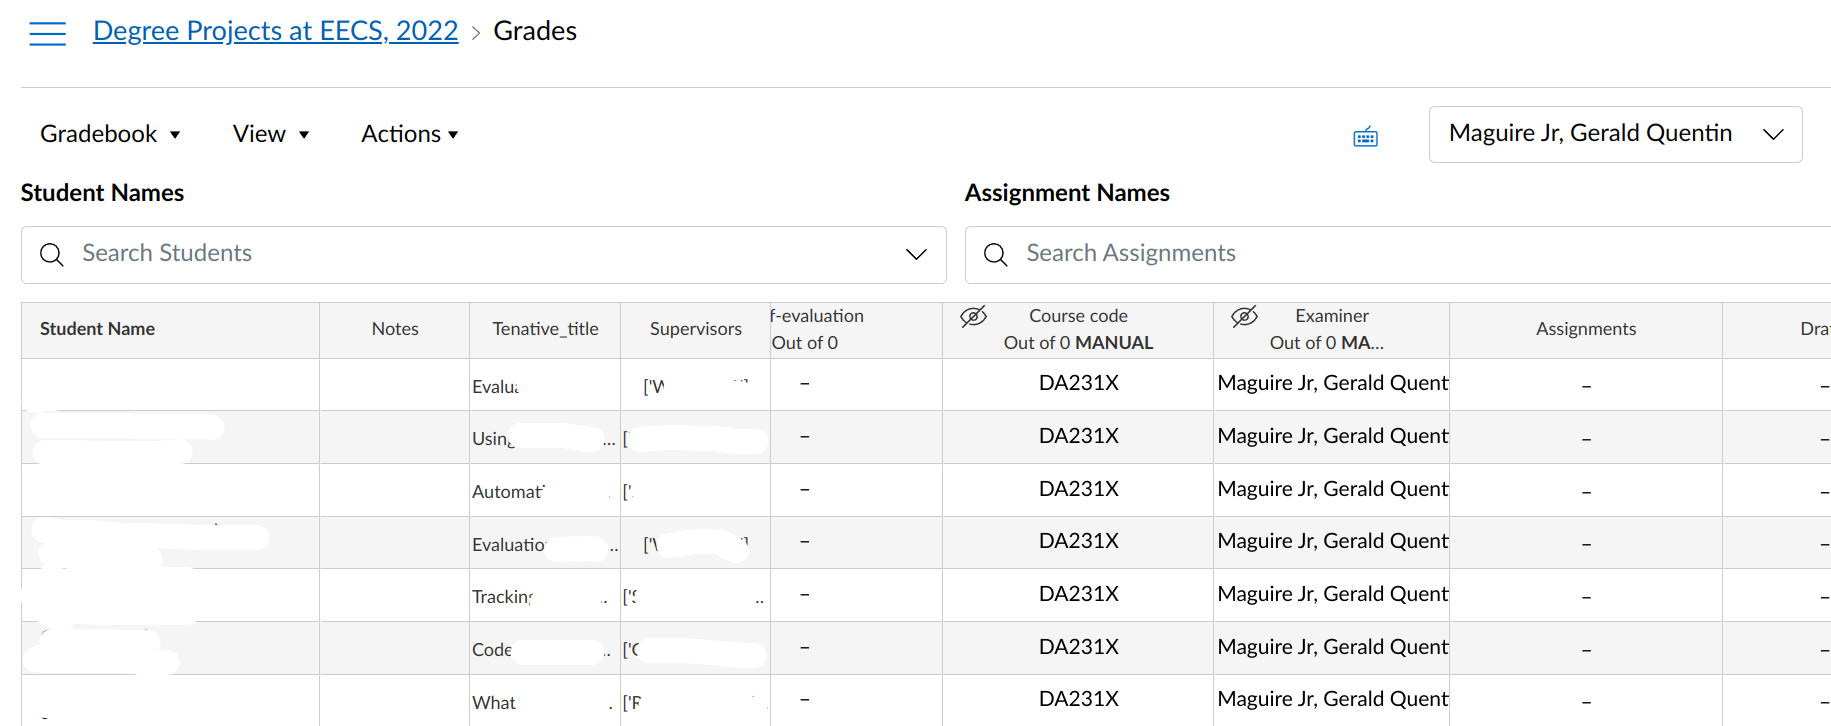
\includegraphics[width=0.99\textwidth]{README_notes/README-examiner-figures/part-of-my-students-Screenshot_20220325_152422-edited.png}
  \end{center}
  \caption{Examiner's view of the gradebook)}
  \label{fig:examinersViewOfGradebook}
\end{figure}

Note that in \Cref{fig:examinersViewOfGradebook}, there are two columns “Course code” and “Examiner”. These are what I call \textit{administrative assignments} and the students do not need to see them (hence the eye symbol with a slash through it – indicating these are hidden from the students). In the “Course code” assignment, I have given the student a “grade” that is the course code of their degree project. This way it is very easy to see what course code a student is enrolled in – as an examiner or supervisor may have students enrolled in several different course codes. This “grading standard”\footnote{What Canvas calls a grading standard is often called a grading scale.} was created from the list of all the EECS 2\textsuperscript{nd} cycle course codes that share this same Canvas course room. The “Examiner” column contains a “grade” that is the name of the examiner assigned for this student. The examiner “grading standard” is created from the list of all of the examiners in the Canvas course room. In the same way that a teacher can assign a grade, if you click on the gradebook cell for a student, you get a pull-down list of all of the possible “grades” in this case the list of examiners, see \Cref{fig:listOfExaminers}.
\begin{figure}[!ht]
  \begin{center}
    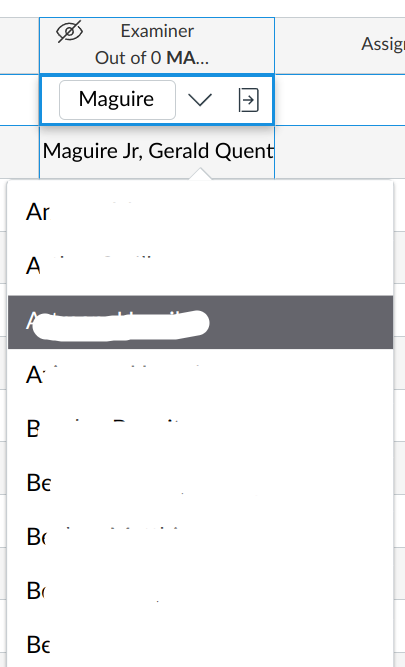
\includegraphics[width=0.5\textwidth]{README_notes/README-examiner-figures/top-of-the-list-of-examiners-Screenshot_20220325_153634.png}
  \end{center}
  \caption[List of examiners]{List of examiners (with the names erased to avoid GDPR problems)}
  \label{fig:listOfExaminers}
\end{figure}

Did I have to manually enter all of the course codes for the 687 students in the course room? No, I used a script via the command shown in \Cref{lst:addCourseCodesForStudentsInCourse}.  This required that initially the grading standard with course codes be created. It was created with the command shown in \Cref{lst:insertCourseCodeGradingStandard}.
\Needspace*{3\baselineskip}
\begin{lstlisting}[language={bash}, caption={add\_course\_codes\_for\_students\_in\_course.py}, label=lst:addCourseCodesForStudentsInCourse]
./add_course_codes_for_students_in_course.py 33514
\end{lstlisting}
\Needspace*{3\baselineskip}
\begin{lstlisting}[language={bash}, caption={insert\_course\_code\_grading\_standard.py}, label=lst:insertCourseCodeGradingStandard]
./insert_course_code_grading_standard.py 33514
\end{lstlisting}
\Needspace*{3\baselineskip}
The grading standard for examiners (and even one for teachers as supervisors) is created with the command shown in  \Cref{lst:insertTeachersGradingStandard}. To create the teachers grading standard you leave off the ``--emaniners'' option.

%% the following conditional is needed to avoid problems with "--" in the listing when using pdflatex
\ifxeorlua
\begin{lstlisting}[language={bash}, caption={insert\_teachers\_grading\_standard.py}, label=lst:insertTeachersGradingStandard]
./insert_teachers_grading_standard.py –-examiners 33514
\end{lstlisting}
\else
\begin{lstlisting}[%language={bash}, 
  basicstyle=\ttfamily, extendedchars=false,
caption={insert\_teachers\_grading\_standard.py}, label=lst:insertTeachersGradingStandard]
./insert_teachers_grading_standard.py –-examiners 33514
\end{lstlisting}
\fi

The command line shown in \Cref{lst:insertTeachersGradingStandard} creates a grading standard with the suffix “\_Examiners”. Note that all of these grading standards are \textit{course specific} grading standards, so they are invisible outside of this course room. One caution about the use of grading standards is that if the list of course codes or list of teachers/examiners changes – there can be problems with the mappings as the grading standard creates a mapping between a numeric grade and a string (the course code or name); therefore, they should only be generated once at the start of the course when the full list of values is known.

So clearly we can have information about the student, supervisors (who are teachers in the course), and examiner in the Canvas course room. Then since these people are in the Canvas course room we can know their sort-able name, KTHID, e-mail address, etc. Clearly, the students were added to the course when they were enrolled in the course. How did the teachers and examiners get into the course? These people were added to the course by a script that IT runs that takes this data from Kurs- och programplaneringssystemet (KOPPS)!

\subsection{How can we associate students with examiners and supervisors?}
In the case of the computer science (CS) students the exjobb coordinator XXXXX\footnote{The person's name has been removed, to avoid issues with GDPR.} has a spreadsheet with the student’s name, working title, examiner, and supervisors in it. It has a sheet named “Closed” that contains information about the students who have been assigned an examiner and supervisor. \Cref{fig:spreadsheetOfCSStudents} shows the column headings of the spreadsheet “Masters\_thesis\_proposals-CS-P3-2022a.xlx” (this is my local file name for the spreadsheet).
	
\begin{figure}[!ht]
  \begin{center}
    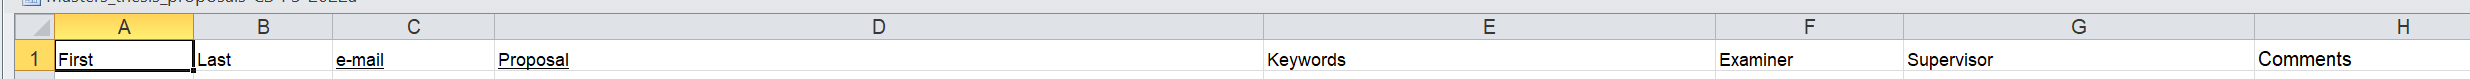
\includegraphics[width=0.99\textwidth]{README_notes/README-examiner-figures/sheet-columns-Screenshot_20220325_155622.png}
  \end{center}
  \caption{Columns in the `Closed' sheet of spreadsheet of CS students)}
  \label{fig:spreadsheetOfCSStudents}
\end{figure}

\Needspace*{6\baselineskip}
A script takes the data from this spreadsheet and adds the information to the Canvas gradebook with the command shown in \Cref{lst:insertExaminersAndSupervisorsFromSpreadsheet}.
\begin{lstlisting}[language={bash}, caption={insert-examiners-and-supervisors-from-spreadsheet.py}, label=lst:insertExaminersAndSupervisorsFromSpreadsheet]
./insert-examiners-and-supervisors-from-spreadsheet.py  33514   "Masters_thesis_proposals-CS-P3-2022a.xlsx"  
\end{lstlisting}
The script uses the student’s e-mail address to look up the student in the Canvas course room, then adds the student to the examiner’s section and updates the “Examiner” grade for this student to show this assigned examiner. It also adds the contents of “Proposal” field from the spreadsheet as text in a custom column in the gradebook called “Tentative\_title” and adds the list of supervisors to the custom column called “Supervisors” – see \Cref{fig:examinersViewOfGradebook}. Note that this program uses a JavaScript Object Notation (JSON) file, \texttt{spreadsheet\_aliases-33514.json}, containing aliases for each of the examiners and supervisors. \Cref{lst:aliasFile} shows part of the alias file.
\Needspace*{15\baselineskip}	
\begin{lstlisting}[language={Python}, caption={Some of the contents of an alias file for a course}, label=lst:aliasFile]
{
    "examiners": {
        "Anders Västberg": "Västberg, Anders",

        "Gerald Maguire": "Maguire Jr, Gerald Quentin",
        "Gerald  Q.  Maguire": "Maguire Jr, Gerald Quentin",

    },
    "teachers": {
    
    }
}
\end{lstlisting}

The alias file takes the names used in the spreadsheet (the name shown on the left in the listing above) and maps them to the sortable names used in Canvas (the name shown on the right in the listing above). While this adds a little more complexity, it addressed the problem that the names used in the spreadsheet are not always consistent or even complete.

The availability of information in Canvas also suggests that some of the arguments that were shown earlier for the script \texttt{create\_customized\_JSON\_file.py} are actually unnecessary and the program can figure them out given the course\_id and student’s e-mail address. However, some things are not accessible directly from Canvas, for example, I have not been able to figure out what exam a student intends to apply for following their degree project course. Another example of missing information is the program code; however, this information is in LADOK and Canvas has the LADOK identifier for each student; however, my script to access LADOK is currently not working.
\Needspace*{8\baselineskip}
\subsection[What happens if I do not have such a spreadsheet?]{What happens if I do not have such\\ a spreadsheet?}

A Canvas administrator can add students to the examiner’s and supervisor’s sections, as shown in \Cref{fig:sectionEntrollments}. Note that the input field can do partial matches on the text that you enter and will give you a list of the partially matching entries and then you can click on one and then click on Update. 
 	
\begin{figure}[!ht]
  \begin{center}
    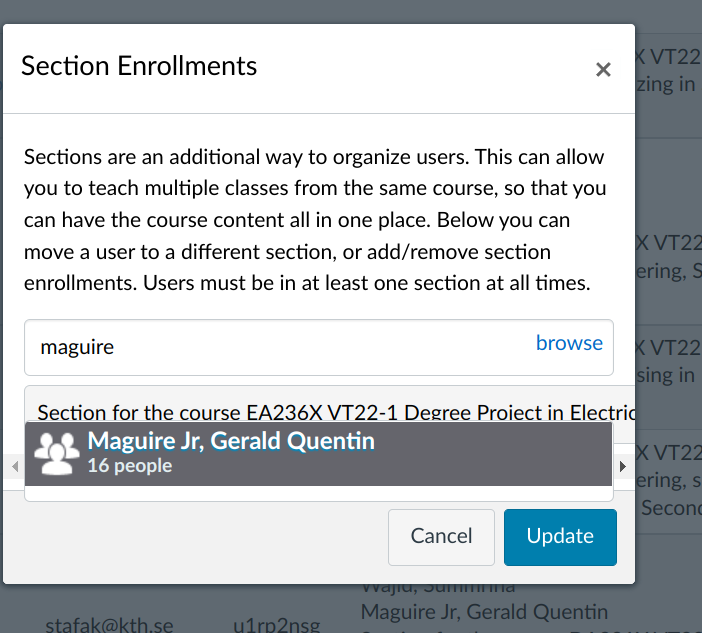
\includegraphics[width=0.99\textwidth]{README_notes/README-examiner-figures/edit-sections-Screenshot_20220325_161529.png}
  \end{center}
  \caption{Section enrollments)}
  \label{fig:sectionEntrollments}
\end{figure}
\FloatBarrier

To get the Section Enrollments editing box popup (shown above) – you go to the “People” page – find the student (either scrolling down the page or starting to type the student’s name in “Search people” box (shown in \Cref{fig:peopleSearchbox}) then click on the vertical three dots on the right side of the row for this student and click on Edit section (as shown in \cref{fig:editSectionsButton}).
\begin{figure}[!ht]
  \begin{center}
    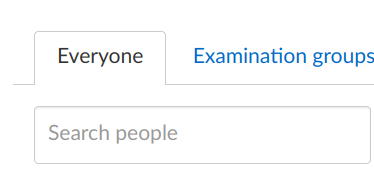
\includegraphics[width=0.5\textwidth]{README_notes/README-examiner-figures/Search-people-Screenshot_20220325_161811.png}
  \end{center}
  \caption{Search people box on People page}
  \label{fig:peopleSearchbox}
\end{figure}
	
\begin{figure}[!ht]
  \begin{center}
    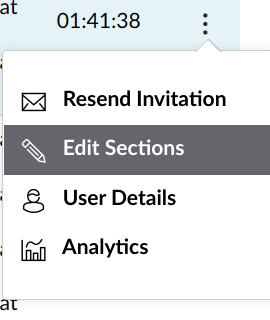
\includegraphics[width=0.5\textwidth]{README_notes/README-examiner-figures/edit-section-cmd-Screenshot_20220325_162252.png}
  \end{center}
  \caption{Three vertical dots and Edit Sections button}
  \label{fig:editSectionsButton}
\end{figure}
\FloatBarrier

Now that we have tied together the student, examiner, and supervisors; we can make use of that information in many ways. One of these ways was to create the customized \LaTeX\;project described earlier. The next section will explain some of the additional steps in the degree project that can be partially automated.
\Needspace*{12\baselineskip}
\section{Automating later steps in the degree project}
\label{sec:AutomatingLaterSteps}
There are many different steps in the degree project that can be facilitated by using the information from the Canvas course room and from the student's thesis. An example of one of these is making an announcement for the student's oral presentation (described in \Cref{sec:makingAnAnnouncement}). Another example is facilitating entering the metadata about the thesis into DiVA (see \Cref{sec:facilitatingDiVAentry}).

\subsection{Making an announcement}
\label{sec:makingAnAnnouncement}
When the examiner has set a time, place, \ldots for the student's oral presentation, then assuming that a student has submitted their thesis with the information in the “For DIVA” pages and that this information includes the information about the opponent(s) and presentation (\eg time, place, zoom link), the steps to make an announcement are:
\begin{enumerate}
    \item Save the PDF file of the thesis, for example \texttt{oscar.pdf}
    \item Extract the “For DIVA” information as JSON, as shown in \Cref{lst:extractPseudoJSONFromPDFforOscarFileToJSON}\footnote{For information about an alternative way to get the JSON file, see \Cref{sec:optimizeJSONToMods}.}
    
    If acronyms are used in the abstracts, you can add the “--acronyms acronyms.tex” argument to the extract command line and the program will process the acronyms from the acronyms.tex file (this means that you will also need this file). The output of the program is a JSON file (oscar.json) that can subsequently be used to make an announcement.
    
    \item Make the announcement for a Canvas course room (in this case, for a Canvas course room with course\_id 11), as shown in \Cref{lst:jsonToCalenarforOscar1}.
    
    Replace 11 with the course\_id of the Canvas course room, for example, 33514 for the EECS 2\textsuperscript{nd} cycle degree projects during 2022.
\end{enumerate}
\Needspace*{7\baselineskip}
\begin{lstlisting}[language={bash}, caption={extract\_pseudo\_JSON-from\_PDF.py for Oscar}, label=lst:extractPseudoJSONFromPDFforOscarFileToJSON]    
   ./extract_pseudo_JSON-from_PDF.py --pdf oscar.pdf --json oscar.json
\end{lstlisting}

\begin{lstlisting}[language={bash}, caption={JSON\_to\_calendar.py for Oscar}, label=lst:jsonToCalenarforOscar1] 
./JSON_to_calendar.py -c 11 --json oscar.json
\end{lstlisting}
The command line shown in \Cref{lst:jsonToCalenarforOscar1} will publish the announcement in \first Canvas course 11, \Second in the Canvas course’s calendar, and \third (eventually) in the KTH Calendar. To publish a KTH calendar event, the software supports the development version of the KTH Cortina API. However, this is API not yet in production and requires a KTH Cortina Access Key.

 For more information see Sections~\ref{sec:whatCanweDoWithTheJSONfile} and \ref{sec:otherVariantsofJSONtoCalendar}.

\subsection{Making a cover and applying it}
\label{sec:makingACover}
As of December 2021, there is a new cover for 1\textsuperscript{st} and 2\textsuperscript{nd} cycle theses at KTH. Information about this is at \url{https://intra.kth.se/en/administration/kommunikation/mallar/avhandlingarochexamensarbeten/skapa-ett-omslag-till-ditt-exjobb-1.479838}.

When the student is writing their thesis, they can set up the title and subtitle in English and Swedish by simply editing the relevant lines in the \LaTeX~file, see \Cref{lst:titleSubtitleEtc}. This is further described in detail in \Cref{sec:putInformationIntoLatexTemplate}  
\iflabelexists{ch:READMEnotes}{and \Cref{ch:READMEnotes}}
{- You have to include the \texttt{README\_notes/README\_notes.tex} file when compiling to get additional information.}

\Needspace*{12\baselineskip}
\begin{lstlisting}[language={[LaTeX]TeX}, caption={Title and subtitle in the two languages}, label=lst:titleSubtitleEtc] 
\title{This is the title in the language of the thesis}
\subtitle{A subtitle in the language of the thesis}

% give the alternative title - i.e., if the thesis is in English, then give a Swedish title
\alttitle{Detta är den svenska översättningen av titeln}
\altsubtitle{Detta är den svenska översättningen av undertiteln}
% alternative, if the thesis is in Swedish, then give an English title
%\alttitle{This is the English translation of the title}
%\altsubtitle{This is the English translation of the subtitle}
  \end{verbatim}
  \caption{Title, subtitle, etc.)}
  \label{fig:titleSubtitleEtc}
\end{lstlisting}

In the case of the \LaTeX\;project, the cover is automatically made and updated as the student writes their thesis. The only things that are needed for the cover that are missing is the exam that the student is going to take out and the TRITA number. We will assume that the student has entered the exam that they are going to apply for in their \LaTeX~file.

Within EECS, the Office of Student Affairs assigns the TRITA number when the examiner has approved the thesis and submitted the PDF file of the approved thesis\footnote{This PDF file is supposed to have the front and back covers; however, as can be seen from the temporal ordering there is a problem as the back cover is made and applied \textbf{before} the number is assigned. One possible solution for this would be to not apply the back cover, but rather have the back cover created and applied by the Office of Student Affairs after they have assigned the TRITA number. Another possible solution would be to tell the examiner the TRITA number so that it can be added to the project and the cover and MODS file made. I think that ideally the TRITA number should be assigned by a program (and stored in a database) and the same program can make and add to the PDF of the thesis. Additionally, the assignments of TRITA numbers in the database can be sent to the archiving unit each year.}. The TRITA number needs to be \first added to the project before generating the final PDF file or \Second alternatively it can be entered by editing the placeholder text on the back cover when the TRITA number is assigned. Note that in the latter case, this data has to be (a) added to the JSON file used to make the MODS file (see \Cref{sec:facilitatingDiVAentry}) or (b) manually edited in DiVA entry.

So what we have seen (in this and other sections) is that we can use the information from Canvas and the thesis itself for simplifying many steps of the degree project process. For example, by having the thesis itself have both the English and Swedish titles and subtitles, it should be easier to add this information to both DiVA and LADOK. The underlying assumption is that the correct and relevant data will be in the Canvas course room and in the thesis itself!
\clearpage

\subsection{To facilitate entering a thesis into DiVA – make a MODS file}
\label{sec:facilitatingDiVAentry}
Assuming that a student has submitted a thesis with the information in the “For DIVA pages” that includes the information for the DIVA entry and the examiner has approved the thesis.

The same steps as described in \Cref{sec:makingACover} are made to save the PDF file and extract the “For DIVA” information as JSON\footnote{For information about an alternative way to get the JSON file, see \Cref{sec:optimizeJSONToMods}.}. This JSON file is then used to make a MODS file via the command shown in \Cref{lst:jsonToMODSforOscar}. Note that in this case, we assume that the person running the program knows the TRITA number; otherwise, the value of the TRITA number in the JSON file is used.
\Needspace*{4\baselineskip}
\begin{lstlisting}[language={bash}, caption={JSON\_to\_MODS.py for Oscar}, label=lst:jsonToMODSforOscar] 
./JSON\_to\_MODS.py -c 11   --json oscar.json --trita "TRITA-EECS-EX-2021:xxxx"
\end{lstlisting}

One way of getting the JSON information to make the MODS file is given in \Cref{sec:optimizeJSONToMods}. A description of how the JSON is converted to a MODS file is given in \Cref{sec:JSONtoMODSfile}.

\section{Can someone else use these programs?}
The source code is at \url{https://github.com/gqmaguirejr/E-learning}. Get the programs from the github, then create a config.json file to provide your Canvas access token and the URL of the Canvas instance you want to use, for details see \url{https://canvas.kth.se/courses/11/pages/making-a-config-dot-json-file-to-make-life-simpler} 

To run the program to make announcements and calendar entries for a course room requires the program and appropriate permissions  to post announcements in a course and insert course calendar events (for example, if the user is a Teacher in the specific Canvas course room or as a Canvas administrator). To make the entry in the KTH Calendar requires a KTH Cortina access key. Making the MODS file does not require any specific permissions as the program is run locally.

To change sections (adding/removing/\ldots a user to/from a section) requires the permissions of a Canvas administrator. However, this is something that E-learning should change about the KTH Canvas configuration; as this should be something that the examiner(s) or course-responsible persons should be able to do. Additionally, the KTH Cortina Calendar API requires an access key (which you have to get from the IT unit).

\Needspace*{12\baselineskip}
\section{\LaTeX~template in Overleaf}
A \LaTeX~template in Overleaf is at \url{https://www.overleaf.com/read/qxvttmmqbgdt} - this is the version used by many EECS students.

Details about using the template are in  
\iflabelexists{ch:READMEnotes}{\Cref{ch:READMEnotes}.}
{xxxx - You have to include the \texttt{README\_notes/README\_notes.tex} file when compiling to get additional information.}
Note that the rest of this document goes into deep detail about \textit{how} the \textbf{template} works and \textit{how} the \textbf{programs} work. The primary intention is to give the information necessary so that someone else can take over the template and programs. Also note that \Cref{sec:accessibility} addresses issues about accessibility.
 
\section{Put information into \LaTeX~template to generate a draft or final thesis}
\label{sec:putInformationIntoLatexTemplate}

\Cref{fig:sampleTitlePage} shows the title page of a fictitious thesis created using a \LaTeX~template that I have developed. The idea is to capture in the thesis itself all of the information needed for this title page, the cover pages, the announcement of the oral presentation, and for reporting the final approved thesis in DiVA via the thesis itself.

\begin{figure}[!ht]
  \begin{center}
    \fbox{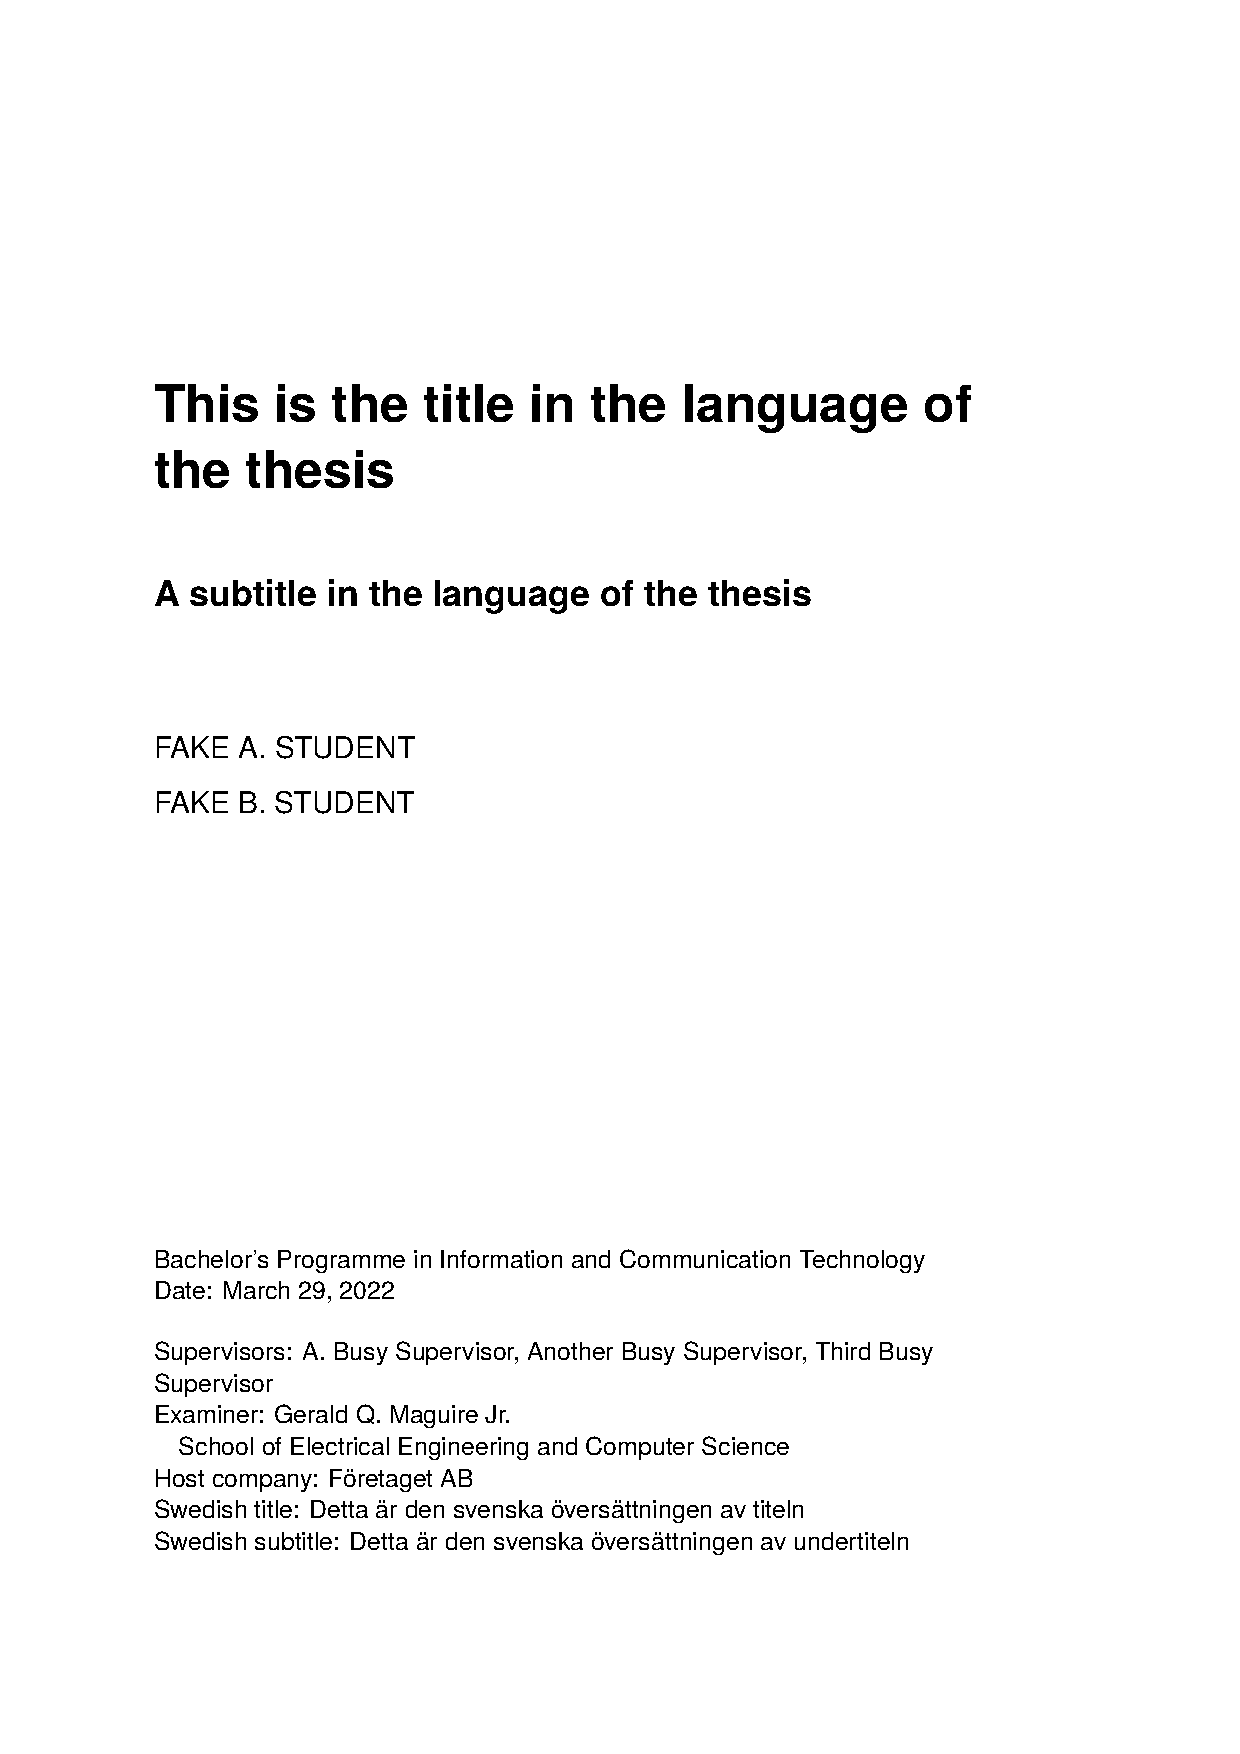
\includegraphics[width=0.85\textwidth]{README_notes/README-examiner-figures/Title-page-20220329.pdf}}
  \end{center}
  \caption{Example of a title page}
  \label{fig:sampleTitlePage}
\end{figure}
\clearpage

For the current documentation of the template for these details, please see the file “README\_notes.tex” in the template itself - 
\iflabelexists{ch:READMEnotes}{\Cref{ch:READMEnotes}.}
{You have to include the \texttt{README\_notes/README\_notes.tex} file when compiling to get additional information.}
What follows includes some older examples – so there may be differences in the details between these examples and the current template.

For the purpose of this document, the following information is present in the order of this exposition, not necessarily the order it is in the \LaTeX~source file. However, all of this information is prior to \textbackslash begin{document}. In particular, information that should be knowable at the start of the degree project is placed into a file named \texttt{custom\_configuration.tex} – to make it easier to pre-configure a project for a student or students (as was described in \Cref{sec:makeItSimpleFromTheStart}).

Information about the title and the student author(s) of the thesis is entered via the set of commands as shown in Listings~\ref{lst:titles} and \ref{lst:authors}. Note that you can have either one or two authors (the latter should generally only occur in the case of a 1\textsuperscript{st} cycle degree project). There are several other elements of metadata collected about the student (primarily driven by the current author metadata fields in DiVA). A brief description of them and why they are there are given below:
\begin{itemize}
    \item One might question why have an e-mail address (when under the current policy is that the student will lose their e-mail address upon graduation)? One of the main reasons is so that the library (\ie KTHB) can notify the student that the thesis has be stored in DiVA. A second reason is if the library needs to contact the student.
    
    \item One might also wonder, why include the student’s \texttt{kthid} (\ie their internal to KTH ID). The main reason is that this identifier \textit{uniquely identifies} this author within KTH, so that all of their publications can be found in a DiVA search. Note that a number of KTH students go on to write papers related to their thesis and a number of these are registered in DiVA. Without a unique identifier, it would not be possible to connect these different documents.
    
    \item A very questionable field is \texttt{authorsSchool}. In a discussion with DiVA administrators at KTH on 2021-04-29, the consensus was that this should be the school of the thesis examiner, since 1\textsuperscript{st} and 2\textsuperscript{nd} cycle students are in \textbf{programs of study} and not schools, department, \etc.
    
    \item Next there is \texttt{programcode} – this is used to generate the degree information just above the other data on the title page and is also used to compute the “lead” for the calendar entry (which differs depending upon whether it is a 1\textsuperscript{st} or 2\textsuperscript{nd} cycle degree project presentation).
    
    \item Finally, the \texttt{degreeName} and \texttt{subjectArea}, \eg \textbackslash degreeName{Bachelors degree} \textbackslash subjectArea{Technology }- provide information that is used later when generating the color KTH cover.
\end{itemize}
\textbf{NB}: A limitation of the current template is that I do not handle the case of two students who are in different programs.

The template previously supported ORCID IDs for students, but as per email from KTH Biblioteket on 2021-06-28, students cannot have an OrCiD reported for their degree project; therefore, this functionality was removed.


An example of information about the title and student authors for a thesis is shown in Listings~\ref{lst:titles} and \ref{lst:authors} (respectively).
\Needspace*{12\baselineskip}
\begin{lstlisting}[language={[LaTeX]TeX}, caption={Information about the titles and subtitles of the thesis}, label=lst:titles]
\title{This is the title in the language of the thesis}
\subtitle{A subtitle in the language of the thesis}

% give the alternative title - i.e., if the thesis is in English, then give a Swedish title
\alttitle{Detta är den svenska översättningen av titeln}
\altsubtitle{Detta är den svenska översättningen av undertiteln}
% alternative, if the thesis is in Swedish, then give an English title
%\alttitle{This is the English translation of the title}
%\altsubtitle{This is the English translation of the subtitle}
\end{lstlisting}
\Needspace*{32\baselineskip}
\begin{lstlisting}[language={[LaTeX]TeX}, caption={Information about the student authors of the thesis}, label=lst:authors] 
\authorsLastname{Student}
\authorsFirstname{Fake A.}
\email{a@kth.se}
\kthid{u100001}
\authorsSchool{\schoolAcronym{EECS}}
%If the student is not in Stockholm, Sweden, add that information here
% This information will be used when generating the acknowledgements signature.
%\authorCity{A City}
%\authorCountry{A Country}
% pass into \authorCityCountryDate{} the month and year for the acknowledgment
% If there is a second author and place, the month, and year are the same, the specify the month and year for the first author:
\authorCityCountryDate{\MONTH\enspace\the\year}
% if there is a second author and the place is different, then say:
%\authorCityCountryDate{}

% If there is a second author - add them here:
\secondAuthorsLastname{Student}
\secondAuthorsFirstname{Fake B.}
\secondemail{b@kth.se}
\secondkthid{u100002}
\secondAuthorsSchool{\schoolAcronym{ABE}}
%If the student is not in Stockholm, Sweden, add that information here
% This information will be used when generating the acknowledgements signature.
%\secondAuthorCity{A City}
%\secondAuthorCountry{A Country}
% pass into \secondAuthorCityCountryDate{} the month and year for the acknowledgement
%\secondAuthorCityCountryDate{\MONTH\enspace\the\year}
%\secondAuthorCityCountryDate{}
\end{lstlisting}


\Cref{lst:hostcompany} shows how to enter data about where the thesis is being done if outside of KTH.
\textbf{NB}: A limitation of the current template is that I do not handle multiple companies, as I assume that there is a single host company. However, you can have a list of names within the two text fields (but only a single \textbackslash hostcompany or a single \textbackslash hostorganization should be included). As of the DiVA administrators meeting of 2022-03-25, if there are a list of names, they should be separated by a semicolon or vertical bar (\ie the `|' character) and the information should be entered in an uniform manner (\ie ``på ett enhetligt sätt''). However, there is not yet a list of the partner names in canonical form. Moreover, it was also noted that if the name of the company or organization is confidential, then the field should contain the string ``Confidential'' and when the DiVA entry is made the actual name or the company or organization should be entered in the ``Internal'' information field (\ie ``intern kommentar'') in DiVA. Unfortunately, it is not clear how the DiVA administrator would know this information. However, 
the KTHB bibliometrics unit is interested in this data, as is the GVS unit working with industrial relations.
\Needspace*{5\baselineskip}
\begin{lstlisting}[language={[LaTeX]TeX}, caption={Information about where the thesis is taking place}, label=lst:hostcompany] 
\hostcompany{Företaget AB} % Remove this line if the project was not done at a host company
%\hostorganization{CERN}   % if there was a host organization
\date{\today}
\end{lstlisting}
\Needspace*{17\baselineskip}
\Cref{lst:oralpresentatioOpponents} collects the information regarding the time, place, and language of the presentation. Note that the opponents' names are simply separated by ‘\&’ – so it is easy to have one more opponent.
\ifxeorlua
\begin{lstlisting}[language={[LaTeX]TeX}, caption={Information relevant to the oral presentation (both the location and the opponent or opponents)}, label=lst:oralpresentatioOpponents] 
%%%%% For the oral presentation
%% Add this information once your examiner has scheduled your oral presentation
\presentationDateAndTimeISO{2022-03-15 13:00}
\presentationLanguage{eng}
\presentationRoom{via Zoom https://kth-se.zoom.us/j/ddddddddddd}
\presentationAddress{Isafjordsgatan 22 (Kistagången 16)}
\presentationCity{Stockholm}

% Opponent's information
\opponentsNames{A. B. Normal \& A. X. E. Normalè}

\nationalsubjectcategories{10201, 10206}
\end{lstlisting}
\else
\begin{lstlisting}[language={[LaTeX]TeX}, extendedchars=false, caption={Information relevant to the oral presentation (both the location and the opponent or opponents)}, label=lst:oralpresentatioOpponents] 
%%%%% For the oral presentation
%% Add this information once your examiner has scheduled your oral presentation
\presentationDateAndTimeISO{2022-03-15 13:00}
\presentationLanguage{eng}
\presentationRoom{via Zoom https://kth-se.zoom.us/j/ddddddddddd}
\presentationAddress{Isafjordsgatan 22 (Kistagången 16)}
\presentationCity{Stockholm}

% Opponent's information
\opponentsNames{A. B. Normal \& A. X. E. Normalè}

\nationalsubjectcategories{10201, 10206}
\end{lstlisting}
\fi
\Needspace*{12\baselineskip}
Finally, \Cref{lst:nationalSubjects} collects the information regarding the National Subject Categories – this is simply a list of 3 or 5 digit numbers separated by commas. The numbers come from \url{https://www.scb.se/contentassets/10054f2ef27c437884e8cde0d38b9cc4/oversattningsnyckel-forskningsamnen.pdf} while the Swedish and English versions are given in \url{https://www.scb.se/contentassets/3a12f556522d4bdc887c4838a37c7ec7/standard-for-svensk-indelning--av-forskningsamnen-2011-uppdaterad-aug-2016.pdf}. This information is for a required field in DiVA. Note that 5 digit codes are preferred over 3 digit codes.
\begin{lstlisting}[language={[LaTeX]TeX}, caption={Information relevant to the oral presentation (both the location and the opponent or opponents}, label=lst:nationalSubjects] 
\nationalsubjectcategories{10201, 10206}
\end{lstlisting}

The program \texttt{create\_customized\_JSON\_file.py} tries to guess the National Subject Categories based upon the particular course code that the student is enrolled in. Currently only the categories that I thought were useful for the EECS 2\textsuperscript{nd} cycle courses codes are well addressed.

\Cref{lst:EnglishAbstractLang} and \Cref{lst:EnglishAbstract} show examples of abstracts that in a real thesis would be in English and Swedish with the first to appear being the abstract in the language of the thesis. Note that the actual content of these two abstracts is primarily for testing and is not meant to suggest real abstracts. However, these examples show some of the equations and symbols that are supported (\ie in the Canvas announcement, calendar postings, and in DiVA).

The template also supports a number of other languages (based on the languages used for abstracts in undergraduate theses in 2020). It is straightforward to add an additional language as necessary. One of the reasons for having abstracts in additional languages is so that dual degree students do not have to write another document for their home/other university. While the template includes a number of placeholders for these other abstracts, if they are unused they can simply be deleted.
The three-character code used for the language is the ISO 639-2 Code – specifically, the "B" (bibliographic) variant of these codes --- as these seem to be the codes used in DiVA when one accesses the MODS formatted metadata for publications. In the example below we see “eng” being stored into a scontents buffer called “lang”.
\Needspace*{5\baselineskip}
\begin{lstlisting}[language={[LaTeX]TeX}, caption={Storing the language in a scontents buffer named "lang"}, label=lst:EnglishAbstractLang] 
\begin{scontents}[store-env=lang]
eng
\end{scontents}
\end{lstlisting}

The abstract itself is stored in an scontents buffer called “abstracts” and the keywords are stored in an scontents buffer called “keywords”.  These buffers are part of the \LaTeX~\texttt{scontents} package and allow contents to be stored and later retrieved. Note that an internal function is used inside this package, so that the abstracts can be stored in raw \LaTeX~code - rather than being stored after being processed. This was done to retain the \LaTeX~codes for mathematics and symbols - so they can be processed into the necessary forms for where they are to be used (\ie in the Canvas announcement, calendar postings, and in DiVA). Further details of the magic of scontents buufers are given in \Cref{sec:scontentsHack}.

\textbf{NB}: Because the raw \LaTeX~code is stored the acronyms need to be processed later by a program (this is described later) - it is suggested that the acronyms be spelled out in the non-English language abstracts, as I do not know how to support them - as multiple language glossaries is not something that I understand how to do nor do I know how to properly generate plurals of Swedish acronyms.

\textbf{NB}: It is assumed that no abstracts or keywords include \textbf{four euro symbols in a row} (\ie quad euro symbols) - as these are used as markers in the file to mark the boundaries of abstracts and lists of keywords.
\Needspace*{34\baselineskip}
\begin{lstlisting}[language={[LaTeX]TeX}, caption={Storing the language in a scontents buffer named "lang"}, label=lst:EnglishAbstract]
\begin{abstract}
  \markboth{\abstractname}{}
\begin{scontents}[store-env=lang]
eng
\end{scontents}
\begin{scontents}[store-env=abstracts,print-env=true]
All theses at KTH are \textbf{required} to have an abstract in both \textit{English} and \textit{Swedish}.

Exchange students may want to include one or more abstracts in the language(s) used in their home institutions to avoid the need to write another thesis when returning to their home institution.

Keep in mind that most of your potential readers are only going to read your \texttt{title} and \texttt{}abstract}. This is why it is important that the abstract give them enough information that they can decide if this document relevant to them or not. Otherwise, the likely default choice is to ignore the rest of your document.

An abstract should stand on its own, i.e., no citations, cross-references to the body of the document, acronyms must be spelled out, … .

Write this early and revise as necessary. This will help keep you focused on what you are trying to do.

Example of a formula in an abstract: $c=2 \cdot \pi \cdot r$ or \[ \int_{a}^{b} x^2 \,dx \]
two chemical formulas: H\textsubscript{2}O or $(C_5O_2H_8)_n$, copyright symbol: \textcopyright Maguire 2021, and some superscripts: \textsuperscript{99m}Tc, A\textsuperscript{*},
A\textsuperscript{\textregistered}, and A\texttrademark.

Write an abstract with the following components:% key parts of the abstract
\begin{itemize}
  \item …

\end{itemize}
% comment at end
\end{scontents}

\subsection*{Keywords}
\begin{scontents}[store-env=keywords,print-env=true]
Canvas Learning Management System, Docker containers, performance tuning
\end{scontents}
\end{abstract}
\end{lstlisting}



\Needspace*{40\baselineskip}
\begin{lstlisting}[language={[LaTeX]TeX}, caption={\LaTeX~input to produce the Swedish abstract}, label=lst:SwedishAbstract] 
 \selectlanguage{swedish} 
\begin{abstract}
    \markboth{\abstractname}{}
\begin{scontents}[store-env=lang]
swe
\end{scontents}
\begin{scontents}[store-env=abstracts,print-env=true]
Alla avhandlingar vid KTH måste ha ett abstrakt på både engelska och svenska.


If you are writing your thesis in English, you can leave this until the final version. If you are writing your thesis in Swedish, then this should be done first – and you should revise as necessary along the way.

If you are writing your thesis in English, this section can be a summary targeted at a more general reader. However, if you are writing your thesis in Swedish, then the reverse is true – your abstract should be for your target audience. Similarly, an English summary can be written targeted at a more general audience.

This means that the English abstract and Swedish sammnfattning  
or Swedish abstract and English summary need not be literal translations of each other.

The abstract in the language used for the thesis should be the first abstract, while the Summary/Sammanfattning in the other language can follow.
\end{scontents}
\subsection*{Nyckelord}
\begin{scontents}[store-env=keywords,print-env=true]
Canvas Lärplattform,Dockerbehållare, prestandajustering
\end{scontents}
\end{abstract}
\end{lstlisting}


\clearpage
\section{Now that data is in the template, what happens?}
\label{sec:nowThatDataIsInTheTemplate}

The first thing that happens is the \LaTeX~code automatically generates one or more pages at the end of the PDF document that contain the data – primarily to be used to report the final approved thesis in DiVA. However, a secondary use is that if this information is added to the draft copy that is going to the opponent – then one can potentially automate many of the steps in announcing the oral presentation (as was described in \Cref{sec:makingAnAnnouncement}).
\Needspace*{8\baselineskip}
Figures~\ref{fig:sampleFOrDIVApage1}, \ref{fig:sampleFOrDIVApage2}, and \ref{fig:sampleFOrDIVApage3} show this “For DIVA” information. The first page is shown as text in \Cref{lst:forDIVApg11Text}. The format is supposed to look like JSON.
For example, the text for the examiner's organization:
\begin{lstlisting}[language=json]
{"organisation": {"L1": "School of Electrical Engineering and Computer Science ",
                 "L2": "Computer Science" }}}
\end{lstlisting}

\noindent is used to determine which local part of the KTH calendar a calendar announcement should appear in, as the Cortina calendar is divided by the school and then by department. Note that the department name must be in Swedish for Cortina.
\clearpage
\begin{figure}[!ht]
  \begin{center}
    \fbox{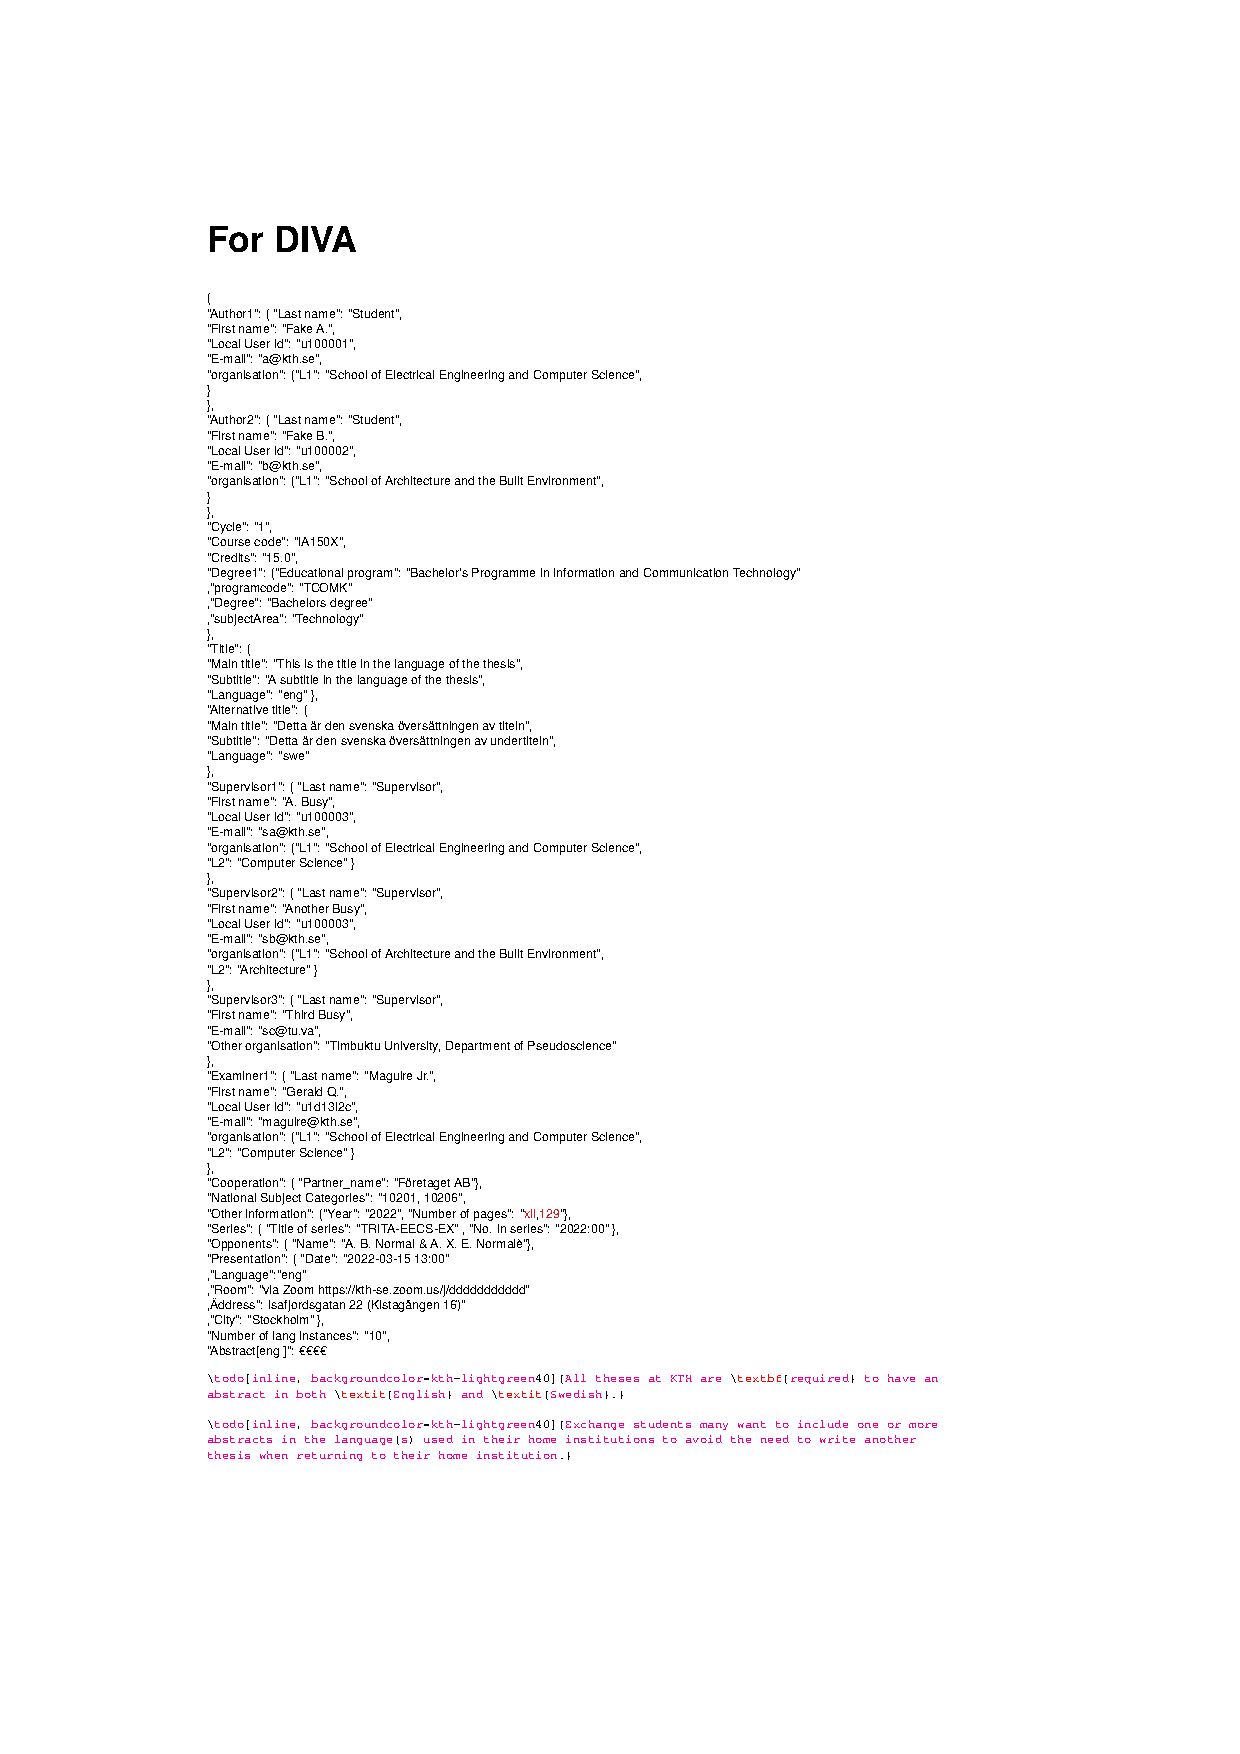
\includegraphics[width=0.85\textwidth]{README_notes/README-examiner-figures/ForDIVA-pg1.pdf}}
  \end{center}
  \caption{First page of the “For DiVA” information}
  \label{fig:sampleFOrDIVApage1}
\end{figure}
\clearpage
\begin{lstlisting}[language={json}, caption={Text version of the first page of the For DIVA output}, label=lst:forDIVApg11Text]
{
"Author1": { "Last name": "Student",
"First name": "Fake A.",
"Local User Id": "u100001",
"E-mail": "a@kth.se",
"organisation": {"L1": "School of Electrical Engineering and Computer Science",
}
},
"Author2": { "Last name": "Student",
"First name": "Fake B.",
"Local User Id": "u100002",
"E-mail": "b@kth.se",
"organisation": {"L1": "School of Architecture and the Built Environment",
}
},
"Cycle": "1",
"Course code": "IA150X",
"Credits": "15.0",
"Degree1": {"Educational program": "Bachelor’s Programme in Information and Communication Technology"
,"programcode": "TCOMK"
,"Degree": "Bachelors degree"
,"subjectArea": "Technology"
},
"Title": {
"Main title": "This is the title in the language of the thesis",
"Subtitle": "A subtitle in the language of the thesis",
"Language": "eng" },
"Alternative title": {
"Main title": "Detta är den svenska översättningen av titeln",
"Subtitle": "Detta är den svenska översättningen av undertiteln",
"Language": "swe"
},
"Supervisor1": { "Last name": "Supervisor",
"First name": "A. Busy",
"Local User Id": "u100003",
"E-mail": "sa@kth.se",
"organisation": {"L1": "School of Electrical Engineering and Computer Science",
"L2": "Computer Science" }
},
"Supervisor2": { "Last name": "Supervisor",
"First name": "Another Busy",
"Local User Id": "u100003",
"E-mail": "sb@kth.se",
"organisation": {"L1": "School of Architecture and the Built Environment",
"L2": "Architecture" }
},
"Supervisor3": { "Last name": "Supervisor",
"First name": "Third Busy",
"E-mail": "sc@tu.va",
"Other organisation": "Timbuktu University, Department of Pseudoscience"
},
"Examiner1": { "Last name": "Maguire Jr.",
"First name": "Gerald Q.",
"Local User Id": "u1d13i2c",
"E-mail": "maguire@kth.se",
"organisation": {"L1": "School of Electrical Engineering and Computer Science",
"L2": "Computer Science" }
},
"Cooperation": { "Partner_name": "Företaget AB"},
"National Subject Categories": "10201, 10206",
"Other information": {"Year": "2022", "Number of pages": "xli,133"},
"Series": { "Title of series": "TRITA-EECS-EX" , "No. in series": "2022:00" },
"Opponents": { "Name": "A. B. Normal & A. X. E. Normalè"},
"Presentation": { "Date": "2022-03-15 13:00"
,"Language":"eng"
,"Room": "via Zoom https://kth-se.zoom.us/j/ddddddddddd"
,"Äddress": Isafjordsgatan 22 (Kistagången 16)"
,"City": "Stockholm" },
"Number of lang instances": "10",
"Abstract[eng ]": €€€€
\engExpl{All theses at KTH are \textbf{required} to have an
abstract in both \textit{English} and \textit{Swedish}.}
\engExpl{Exchange students many want to include one or more
abstracts in the language(s) used in their home institutions to avoid the need to write another
thesis when returning to their home institution.}
\end{lstlisting}
\clearpage
\begin{figure}[!ht]
  \begin{center}
    \fbox{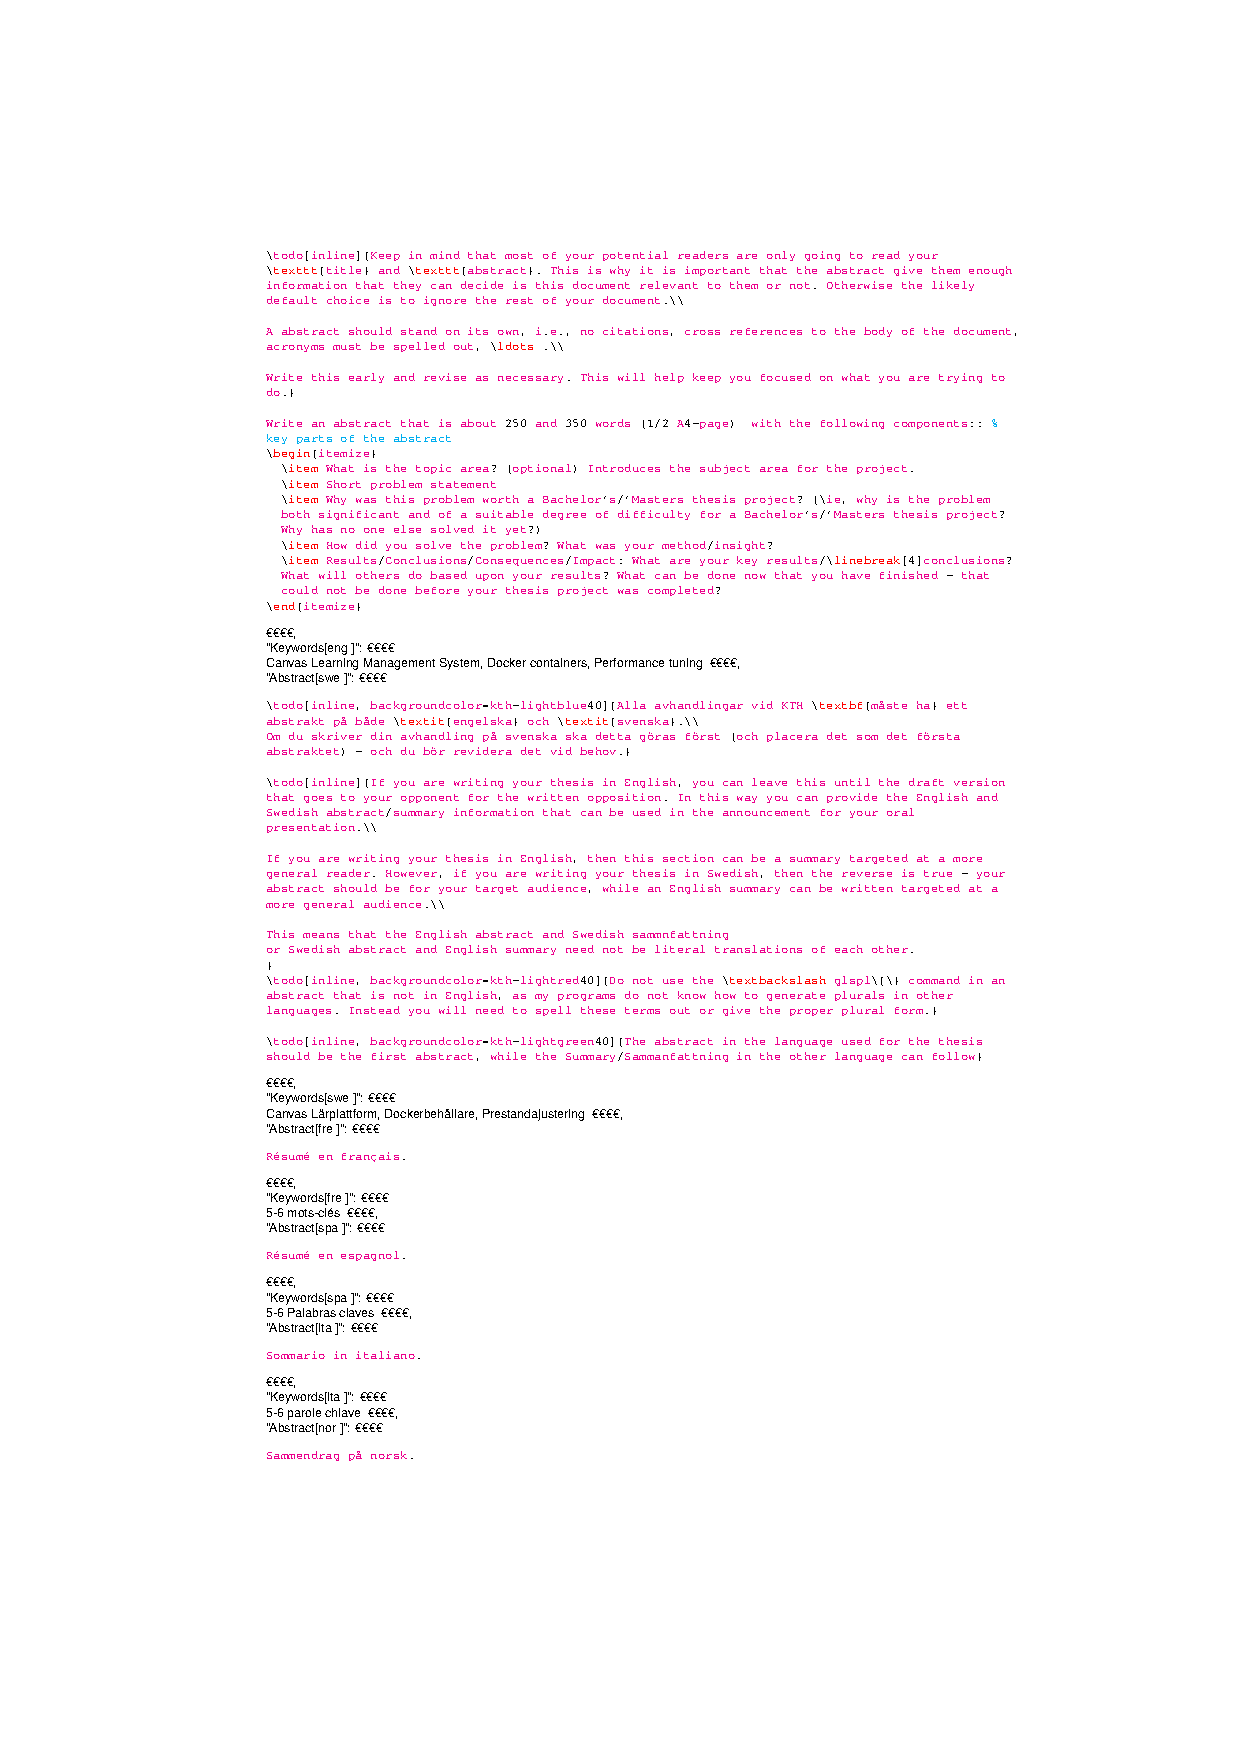
\includegraphics[width=0.80\textwidth]{README_notes/README-examiner-figures/ForDIVA-pg2.pdf}}
  \end{center}
  \caption{Second page of the “For DiVA” information}
  \label{fig:sampleFOrDIVApage2}
\end{figure}
\begin{figure}[!ht]
  \begin{center}
    \fbox{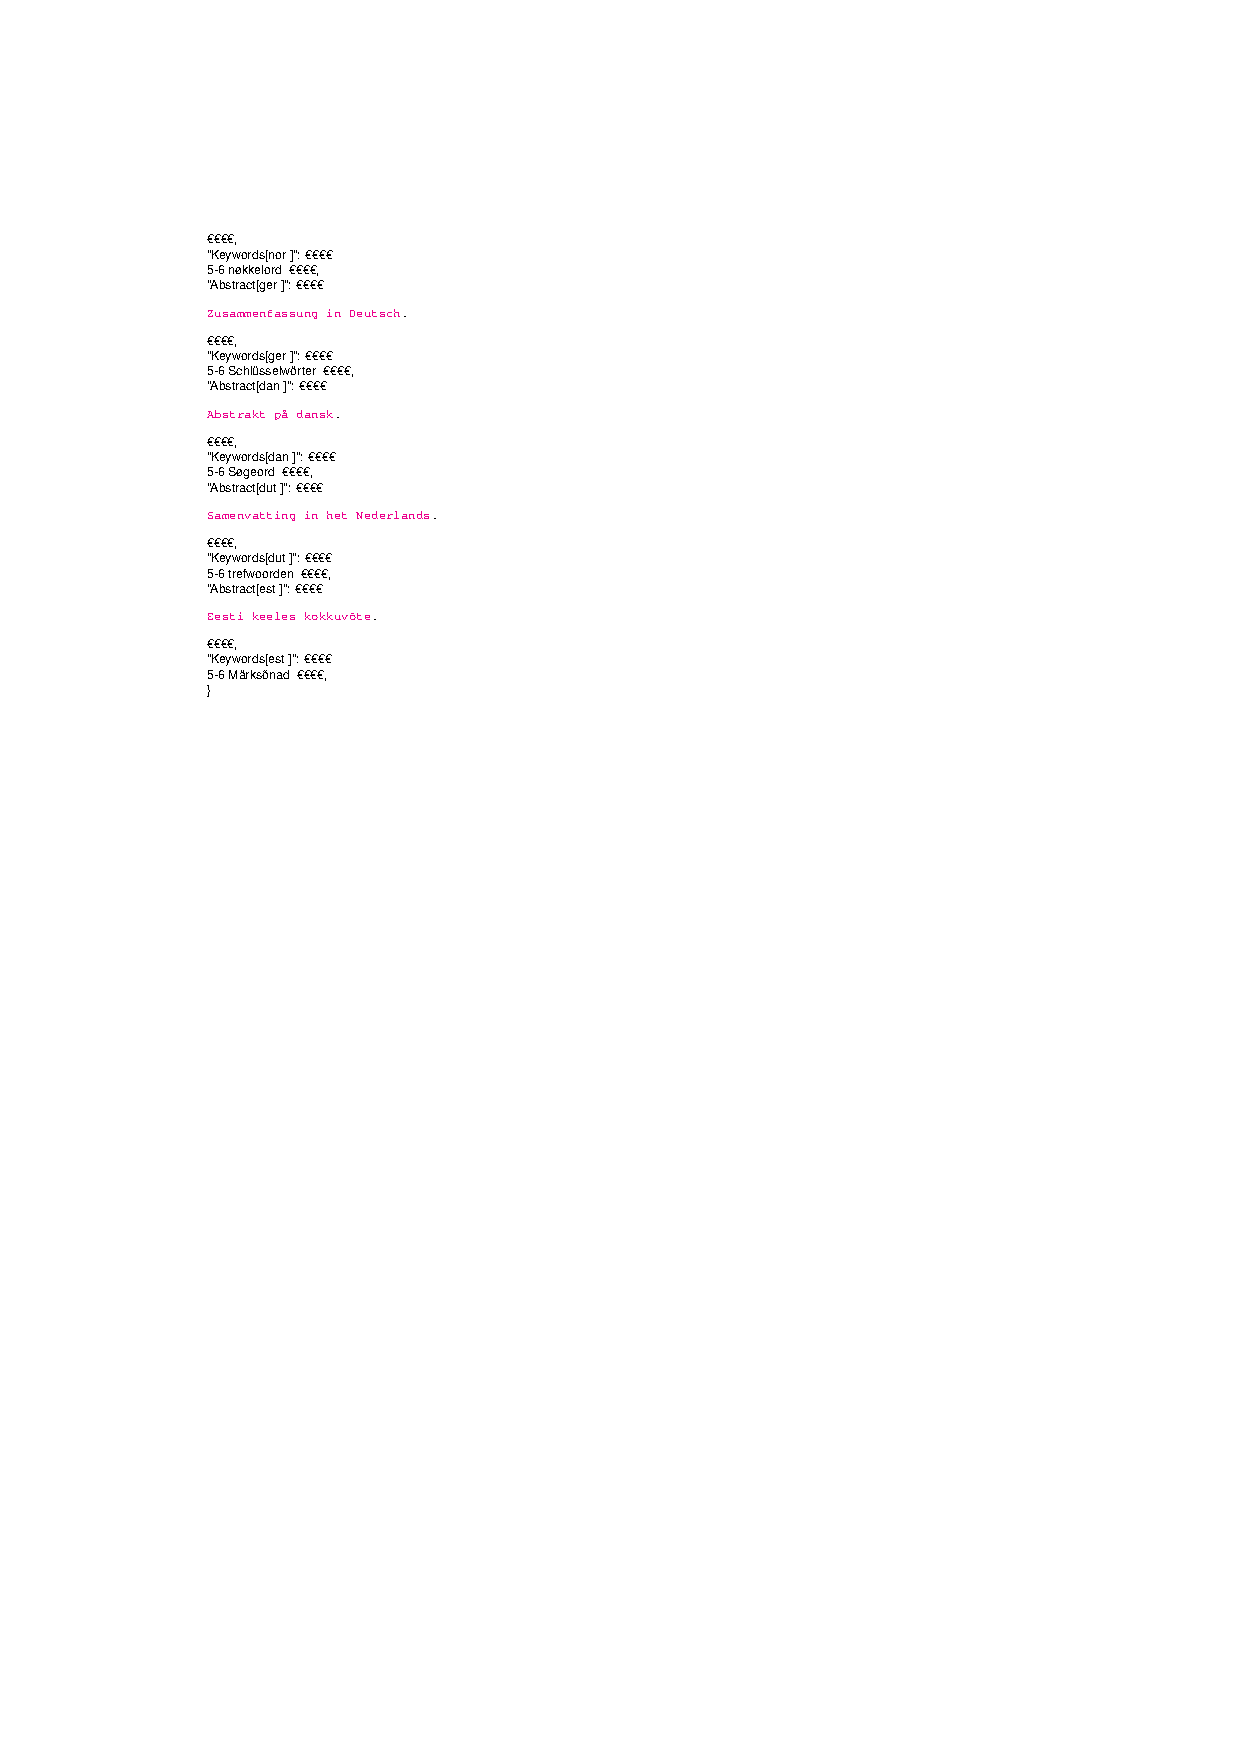
\includegraphics[width=0.80\textwidth]{README_notes/README-examiner-figures/ForDIVA-pg3.pdf}}
  \end{center}
  \caption{Third page of the “For DiVA” information}
  \label{fig:sampleFOrDIVApage3}
\end{figure}
\clearpage
\FloatBarrier


\section{How did the abstracts and the keywords appear?}
\label{sec:scontentsHack}
The \textbackslash divainfo command that generates the For DiVA information pages has the following little bit of code that walks the set of scontents buffers using the lang scontents buffer to put the language and the corresponding abstract and keywords (see \Cref{lst:languages}). Originally, I used \textbackslash getstored[\textbackslash i]{abstracts} to get an abstract, but this turns out to process the \LaTeX~into something to render in the PDF. However, I realized that it would be far better to get the actual \LaTeX~source code and then process it myself into HTML for the announcement and calendars.

The \textbackslash typestored command that the scontents package provides will not take a variable argument, \ie it only takes a constant, such as \textbackslash typestored[2]{abstracts}. Unfortunately, I need to have a loop to handle the variable number of abstracts that could be used. To do this required a new command \textbackslash typestoredx that evaluates the variable and then calls the internal function that gets the contents of the correct scontents buffer! This new command is shown in \Cref{lst:languages} – it uses ExplSyntax – see the \LaTeX~package \texttt{expl3}. The quad euro symbols are used as markers to avoid problems with quotation marks in the abstract itself. I have assumed that such a combination of characters will \textbf{never} occur in an abstract.
\Needspace*{11\baselineskip}
\begin{lstlisting}[language={[LaTeX]TeX}, caption={Code in \textbackslash divainfo command to output the abstracts and keywords }, label=lst:languages] 
    "Number of lang instances": \textquotedbl\relax\countsc{lang}\textquotedbl\relax,\\
    \foreach \i in {1,...,\countsc{lang}} {
      "Abstract[\getstored[\i]{lang}]": €€€€\\
      \typestoredx{\i}{abstracts}
      €€€€,\\
      "Keywords[\getstored[\i]{lang}]": €€€€\\
      \getstored[\i]{keywords}
      €€€€,\\
    }
\end{lstlisting}

\Cref{lst:setupTypestoreedx} shows how to configure the listings environment to put the abstract into. One of the tricks here is that it was important to reduce the hyphenation penalty to enable the abstract text to nicely wrap text on the page. As an added benefit, the \LaTeX~syntax highlighting is on – so one can easily see the \LaTeX~commands that are used – as they might need manual editing before the event is announced. The \LaTeX~code for the English and Swedish abstracts is shown in \Cref{lst:latexAbtractsExampleEnglish} and \Cref{lst:latexAbtractsExampleSwedish} (respectively).

\begin{lstlisting}[language={[LaTeX]TeX}, caption={Code in the document file to set up the command \textbackslash typestoredx and to configure the listing environment to put the abstract into}, label=lst:setupTypestoreedx] 
\ExplSyntaxOn
\newcommand\typestoredx[2]{\expandafter\__scontents_typestored_internal:nn\expandafter{#1} {#2}}
\ExplSyntaxOff
\makeatletter
\let\verbatimsc\@undefined
\let\endverbatimsc\@undefined
\lst@AddToHook{Init}{\hyphenpenalty=50\relax}
\makeatother


\lstnewenvironment{verbatimsc}
    {
    \lstset{%
        basicstyle=\ttfamily\tiny,
        %basicstyle=\tiny,
        %columns=fullflexible,
        columns=[l]fixed,
        language=[LaTeX]TeX,
        %numbers=left,
        %numberstyle=\tiny\color{gray},
        keywordstyle=\color{red},
        breaklines=true,                 % sets automatic line breaking
        breakatwhitespace=true,          % sets if automatic breaks should only happen at whitespace
        %keepspaces=false,
        breakindent=0em,
        %fancyvrb=true
    }
}{}
\end{lstlisting}
\clearpage

\begin{lstlisting}[language={[LaTeX]TeX}, caption={\LaTeX~code for the English abstract}, label=lst:latexAbtractsExampleEnglish] 
\engExpl{All theses at KTH are \textbf{required} to have an
abstract in both \textit{English} and \textit{Swedish}.}
\engExpl{Exchange students many want to include one or more
abstracts in the language(s) used in their home institutions to avoid the need to write another
thesis when returning to their home institution.}
\generalExpl{Keep in mind that most of your potential readers are only going to read your
\texttt{title} and \texttt{abstract}. This is why it is important that the abstract give them enough
information that they can decide if this document is relevant to them or not. Otherwise, the likely
default choice is to ignore the rest of your document.\\
An abstract should stand on its own, i.e., no citations, cross-references to the body of the document,
acronyms must be spelled out, \ldots .\\
Write this early and revise as necessary. This will help keep you focused on what you are trying to
do.}
Write an abstract that is about 250 and 350 words (1/2 A4-page) with the following components:: %
key parts of the abstract
\begin{itemize}
\item What is the topic area? (optional) Introduces the subject area for the project.
\item Short problem statement
\item Why was this problem worth a Bachelor’s/’Masters thesis project? (\ie, why is the problem
both significant and of a suitable degree of difficulty for a Bachelor’s/’Masters thesis project?
Why has no one else solved it yet?)
\item How did you solve the problem? What was your method/insight?
\item Results/Conclusions/Consequences/Impact: What are your key results/\linebreak[4]conclusions?
What will others do based on your results? What can be done now that you have finished - that
could not be done before your thesis project was completed?
\end{itemize}
\end{lstlisting}

\begin{lstlisting}[language={[LaTeX]TeX}, caption={\LaTeX~code for the Swedish abstract}, label=lst:latexAbtractsExampleSwedish]
\todo[inline, backgroundcolor=kth-lightblue40]{Alla avhandlingar vid KTH \textbf{måste ha} ett
abstrakt på både \textit{engelska} och \textit{svenska}.\\
Om du skriver din avhandling på svenska ska detta göras först (och placera det som det första
abstraktet) - och du bör revidera det vid behov.}
\generalExpl{If you are writing your thesis in English, you can leave this until the draft version
that goes to your opponent for the written opposition. In this way you can provide the English and
Swedish abstract/summary information that can be used in the announcement for your oral
presentation.\\
If you are writing your thesis in English, then this section can be a summary targeted at a more
general reader. However, if you are writing your thesis in Swedish, then the reverse is true – your
abstract should be for your target audience, while an English summary can be written targeted at a
more general audience.\\
This means that the English abstract and Swedish sammnfattning
or Swedish abstract and English summary need not be literal translations of each other.
}
\warningExpl{Do not use the \textbackslash glspl\{\} command in an
abstract that is not in English, as my programs do not know how to generate plurals in other
languages. Instead you will need to spell these terms out or give the proper plural form.}
\engExpl{The abstract in the language used for the thesis
should be the first abstract, while the Summary/Sammanfattning in the other language can follow}
\end{lstlisting}

\section{Extracting the information from the PDF file}
Now that the JSON-like information is in the PDF file, the next step is to extract it. The command line shown in \Cref{lst:extractPseudoJSONfromPDF-event} will extract the information. \Cref{lst:JSONfromPDF-event} shows an example of the resulting file.
\begin{lstlisting}[language={bash}, caption={Extract the JSON like information}, label=lst:extractPseudoJSONfromPDF-event]
./extract_pseudo_JSON-from_PDF.py --pdf test5.pdf --json event.json
\end{lstlisting}

\begin{lstlisting}[language={HTML}, caption={Example event.json output (note that this is not the same as currently extracted and note that some lines have been edited and manually broken to overcome limited line length in listing)}, label=lst:JSONfromPDF-event]
{"Author1": {"Last name": "Student", "First name": "Fake A.", "Local User Id": "u100001", "E-mail": "a@kth.se", "organisation": {"L1": "School of Electrical Engineering and Computer Science "}},
"Author2": {"Last name": "Student", "First name": "Fake B.", "Local User Id": "u100002", "E-mail": "b@kth.se", "organisation": {"L1": "School of Architecture and the Built Environment "}},
"Degree": {"Educational program": "Bachelor’s Programme in Information and Communication Technology"},
"Title": {"Main title": "This is the title in the language of the thesis", "Subtitle": "An subtitle in the language of the thesis", "Language": "eng"},
"Alternative title": {"Main title": "Detta är den svenska översättningen av titeln", "Subtitle": "Detta är den svenska översättningen av undertiteln", "Language": "swe"},
"Supervisor1": {"Last name": "Supervisor", "First name": "A. Busy", "Local User Id": "u100003", "E-mail": "sa@kth.se", "organisation": {"L1": "School of Electrical Engineering and Computer Science ", "L2": "Computer Science"}},
"Supervisor2": {"Last name": "Supervisor", "First name": "Another Busy", "Local User Id": "u100003", "E-mail": "sb@kth.se", "organisation": {"L1": "School of Architecture and the Built Environment ", "L2": "Public Buildings"}},
"Examiner1": {"Last name": "Maguire Jr.", "First name": "Gerald Q.", "Local User Id": "u100004", "E-mail": "maguire@kth.se", "organisation": {"L1": "School of Electrical Engineering and Computer Science ", "L2": "Computer Science"}},
"Cooperation": {"Partner_name": "Företaget AB"}, "Other information": {"Year": "2021", "Number of pages": "xxxiii,35"},
"Opponents": {"Name": "A. B. Normal & A. X. E. Normalè"},
"Presentation": {"Date": "2021-03-16 13:00", "Language": "eng", "Room": "via Zoom", "City": "Stockholm"},
"Number of lang instances": "10",
"abstracts": {"eng": "<p>All theses at KTH are <bold>required</bold> to have an abstract in both <i>English</i> and <i>Swedish</i>.</p><p>Exchange students many want to include one or more abstracts in the language(s) used in their home institutions to avoid the need to write another thesis when returning to their home institution.</p><p>Keep in mind that most of your potential readers are only going to read your <tt>title</tt> and <tt>abstract</tt>. This is why it is important that the abstract give them enough information that they can decide is this document relevant to them or not. Otherwise the likely default choice is to ignore the rest of your document.</p><p>A abstract should stand on its own, i.e., no citations, cross references to the body of the document, acronyms must be spelled out, … .</p><p>Write this early and revise as necessary. This will help keep you focused on what you are trying to do.</p><p>Example of a formula in an abstract: $c=2 \\cdot \\pi \\cdot r$ or \\[ \\int_{a}^{b} x^2 \\,dx \\] two chemical formulas: H<sub>2</sub>O or $(C_5O_2H_8)_n$, copyright symbol: &copy; Maguire 2021, and some superscripts: <sup>99m</sup>Tc, A<sup>*</sup>, A<sup>&reg;</sup>, and A&trade;.</p><p>Write an abstract with the following components: </p><ul><li> What is the topic area? (optional) Introduces the subject area for the project. </li><li> Short problem statement </li><li> Why was this problem worth a ’Masters thesis project? (i.e., why is the problem both significant and of a suitable degree of difficulty for a ’Masters thesis project? Why has no one else solved it yet?) </li><li> How did you solve the problem? What was your method/insight? </li><li> Results/Conclusions/Consequences/Impact: What are your key results/conclusions? What will others do based upon your results? What can be done now that you have finished - that could not be done before your thesis project was completed?</li></ul>",
"swe": "<p>Alla avhandlingar vid KTH måste ha ett abstrakt på både engelska och svenska.</p><p>If you are writing your thesis in English, you can leave this until the final version. If you are writing your thesis in Swedish then this should be done first – and you should revise as necessary along the way.</p><p>If you are writing your thesis in English, then this section can be a summary targeted at a more general reader. However, if you are writing your thesis in Swedish, then the reverse is true – your abstract should be for your target audience, while an English summary can be written targeted at a more general audience.</p><p>This means that the English abstract and Swedish sammnfattning or Swedish abstract and English summary need not be literal translations of each other.</p><p>The abstract in the language used for the thesis should be the first abstract, while the Summary/Sammanfattning in the other language can follow.</p>",
"fre": "<p>Résumé en français.</p>", "spa": "<p>Résumé en espagnol.</p>", "ita": "<p>Sommario in italiano.</p>",
"nor": "<p>Sammendrag på norsk.</p>", "ger": "", "dan": "<p>Abstrakt på dansk.</p><p>Zusammenfassung in Deutsch.</p>",
"dut": "<p>Samenvatting in het Nederlands.</p><p>Eesti keeles kokkuvõte.</p>", "est": ""},
"keywords": {"eng": "Canvas Learning Management System, Docker containers, performance tuning ",
"swe": "Canvas Lärplattform,Dockerbehållare, prestandajustering ", "fre": "5-6 mots-clés ",
"spa": "5-6 Palabras claves ", "ita": "5-6 parole chiave ", "nor": "5-6 nøkkelord ",
"ger": "5-6 Schlüsselwörter ", "dan": "5-6 Søgeord ",
"dut": "5-6 trefwoorden ", "est": "5-6 Märksõnad "}}
\end{lstlisting}
\FloatBarrier

\section{Optimized extraction from an Overleaf LaTeX project}
\label{sec:optimizeJSONToMods}
In the case of an Overleaf project, when compiling the \LaTeX~\ as a side-effect, a \texttt{fordiva.json} file is generated, if you save this file locally, then you can clean it up and make a MODS file with the following commands:
\Needspace*{4\baselineskip}
\begin{lstlisting}[language={bash}, caption={cleanup\_pseudo\_JSON-from\_LaTeX and JSON\_to\_MODS.p},label=lst:cleanPseudoJSONandConvertToMODS]
./cleanup_pseudo_JSON-from_LaTeX.py --json xxx_fordiva.json --acronyms acronyms.tex
./JSON_to_MODS.py --json xxx_fordiva.json
\end{lstlisting}

Now all you have to do is rename the XML file that was produced to \texttt{xxx.mods} and you are all set to upload it into DiVA!

To find the \texttt{fordiva.json} file, look for the “Other logs and files” button shown at the bottom of the log output window. This button is shown in \Cref{fig:otherLogfiles}. After clicking this button you will see a list of log and other files, such as shown in \ref{fig:filesProduced}.
	
\begin{figure}[!ht]
  \begin{center}
    \fbox{
\includegraphics[width=0.80\textwidth]{README_notes/README-examiner-figures/otherlog_files.png}}
  \end{center}
  \caption{Other logs and files button}
  \label{fig:otherLogfiles}
\end{figure}

The details for how the \texttt{fordiva.json} file is generated are given in \Cref{sec:AlternativeWayofGeneratingJSON}.

 \begin{figure}[!ht]
  \begin{center}
    \fbox{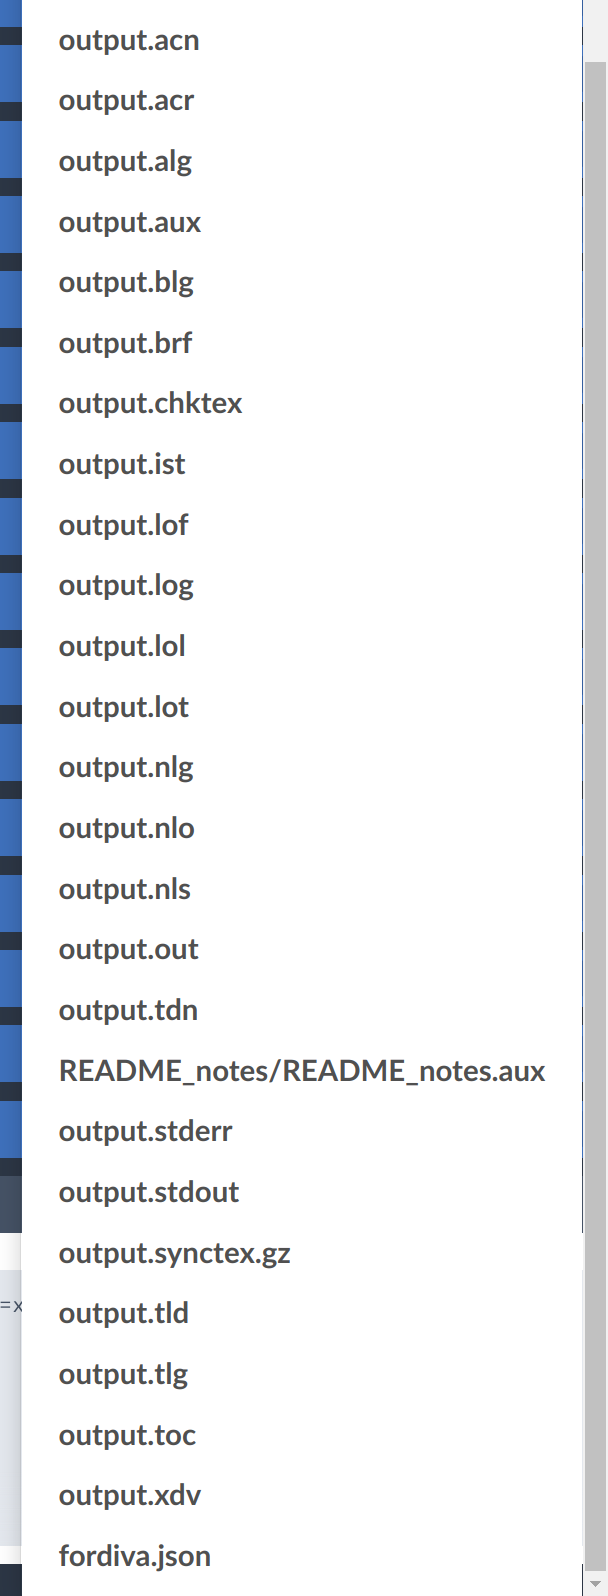
\includegraphics[width=0.50\textwidth]{README_notes/README-examiner-figures/files-produced-Screenshot_20220326_181731.png}}
  \end{center}
  \caption{List of log and other files}
  \label{fig:filesProduced}
\end{figure}
\clearpage

\section{What can we do with the JSON file?}
\label{sec:whatCanweDoWithTheJSONfile}
Now that we have a JSON file, you can edit the HTML in the abstracts to deal with equations and things that were not automatically processed by the extraction program. Once you are happy with the JSON file’s contents, the next step is to generate something interesting with this data – for this we use the program JSON\_to\_calendar.py. 



 \begin{figure}[!ht]
\begin{tikzpicture}
[align=left,node distance=2cm]
\node (jsonFile) [tape,tape bend top=none,draw,font=\sffamily] {JSON file};
\node (start) [processBox, right=1cm of jsonFile] {JSON\_to\_calendar};

\node (calendarEvent) [destinationBox, right=2cm of start] {Canvas calendar event};
\node (announcement) [destinationBox,  above of =calendarEvent] {Canvas announcement};
\node (cortinaCalendarEvent) [destinationBox,  right=0.5cm of start, below of=calendarEvent] {KTH Cortina calendar event};
\draw [arrow] (jsonFile) --  (start.west);
\draw [arrow] (start.east) --  (announcement.west);
\draw [arrow] (start.east) -- (calendarEvent);
\draw [arrow] (start.east) -- (cortinaCalendarEvent.west);

\end{tikzpicture}
\caption{The several outputs of JSON\_to\_calendar.py given a JSON file}
  \label{fig:foo}
\end{figure}
\FloatBarrier

We can produce all three outputs with the command shown in \Cref{lst:JSONtoCalendarThreeoutputs}. Note that the program was run with the \texttt{event.json} file to produce a Canvas course announcement, as shown in \Cref{fig:canvasCourseAnnouncement}. Note that this is being run in the Canvas test instance (hence the pink bar across the bottom of the figure).
\Needspace*{3\baselineskip}
\begin{lstlisting}[language={bash}, caption={Running JSON\_to\_calendar.py to produce all three outputs}, label=lst:JSONtoCalendarThreeoutputs]
JSON_to_calendar.py -c 11 --config config-test.json
\end{lstlisting}

When the cover generator website existed, this same basic mechanism was extended to make and apply the cover for a thesis. There is still a need for a tool that can automate the insertion of the final thesis and metadata into DiVA. While a prototype was shown earlier for this, the IT unit wants to wait for a DiVA API from the DiVA organization. However, an alternative is to generate a MODS file that can be manually imported into DiVA. The process for this will be discussed in \Cref{sec:JSONtoMODSfile}.
\clearpage
\begin{figure}[!ht]
  \begin{center}
    \fbox{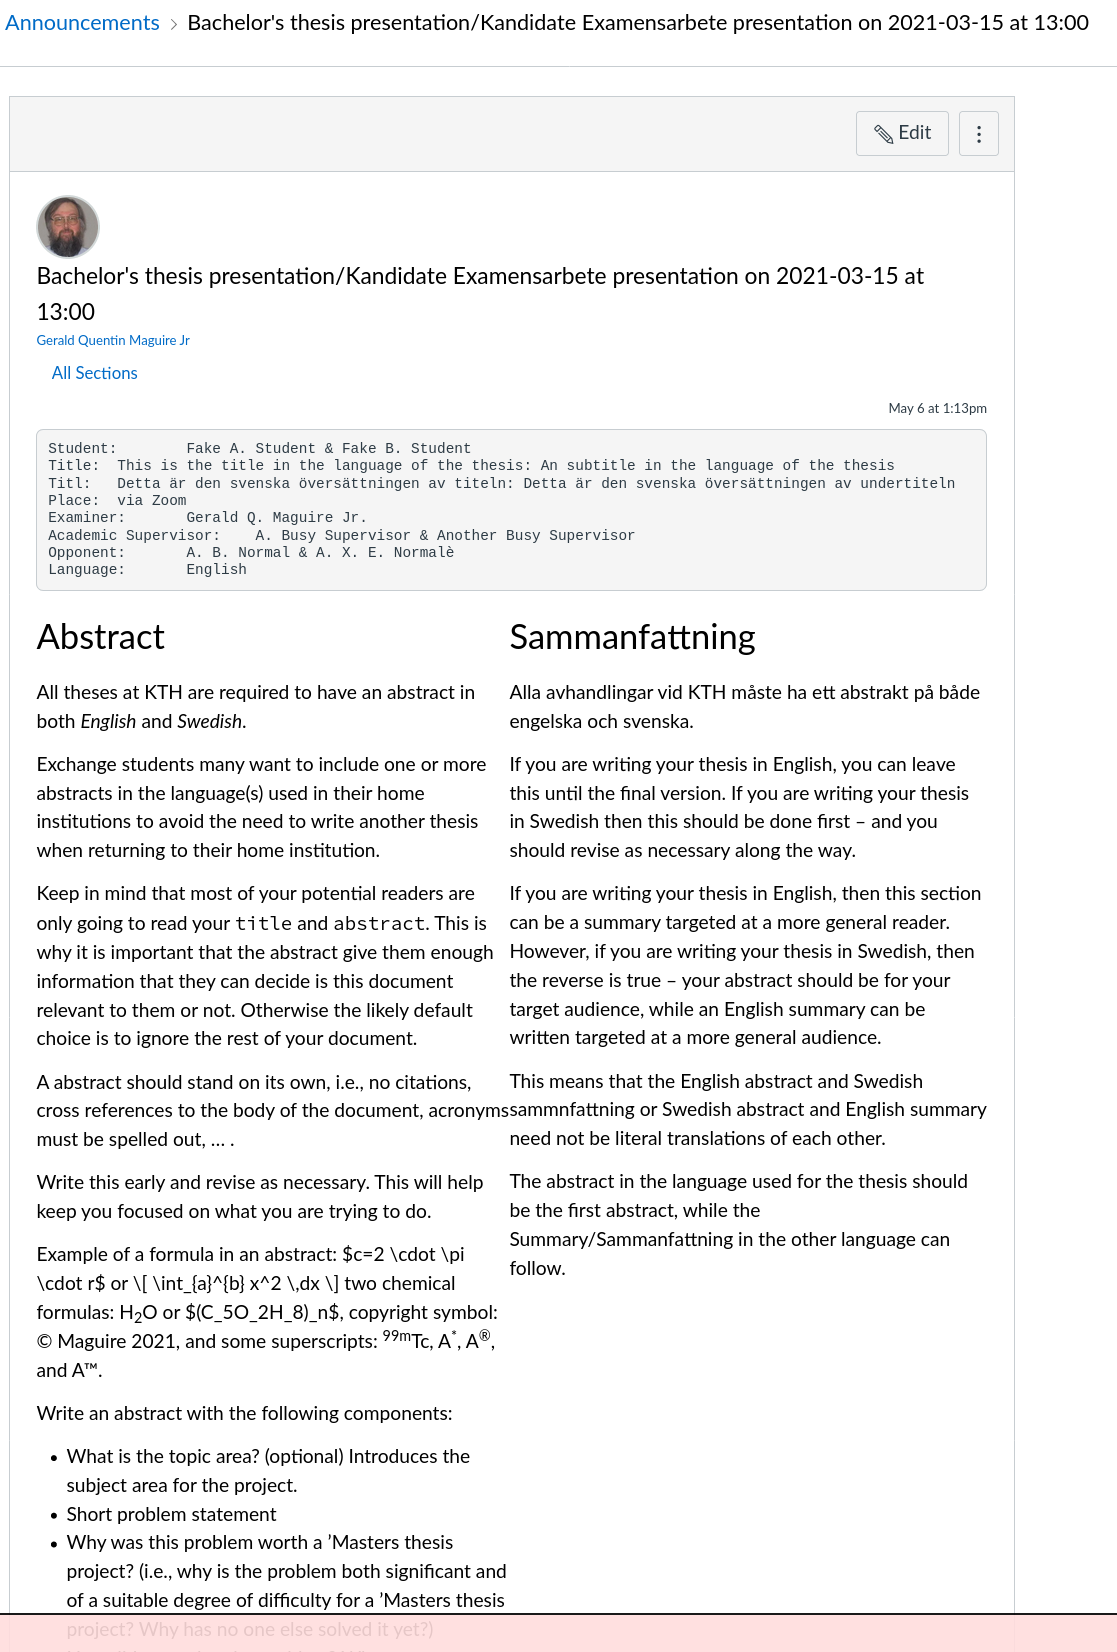
\includegraphics[width=0.99\textwidth]{README_notes/README-examiner-figures/Announcement-in-Canvas-course-Screenshot_20210506_133101.png}}
  \end{center}
  \caption{Canvas course announcement}
  \label{fig:canvasCourseAnnouncement}
\end{figure}
\clearpage
\Cref{fig:canvasCourseAnnouncement} and \Cref{fig:canvasCalendarEvent}  show the event in the Canvas calendar (when I have selected to display the events for course 11 in green).
\begin{figure}[!ht]
  \begin{center}
    \fbox{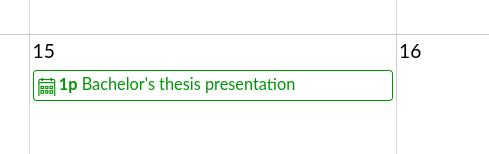
\includegraphics[width=0.60\textwidth]{README_notes/README-examiner-figures/Event-in-Canvas-course-calendar-Screenshot_20210506_133011.png}}
  \end{center}
  \caption{A course event in the Canvas calendar (the figure is zoomed in on 15 March 2021}
  \label{fig:canvasCalendarEvent}
\end{figure}

\begin{figure}[!hb]
  \begin{center}
    \fbox{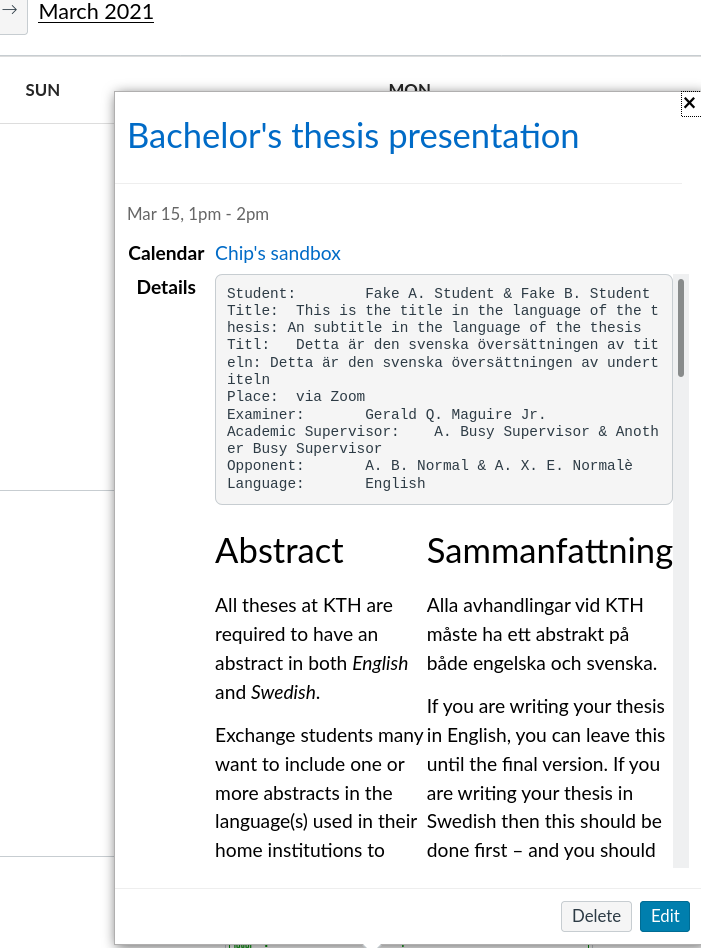
\includegraphics[width=0.70\textwidth]{README_notes/README-examiner-figures/Canvas-calenda-zoomed-open-event-Screenshot_20210506_163851.png}}
  \end{center}
  \caption{Zoomed view of the opened Canvas calendar event}
  \label{fig:canvasCalendarEventZoomed}
\end{figure}
\newpage

I also edited the \texttt{event.json} to create an event on the following date. The result is two Calendar events as shown in \Cref{fig:cortinaPicture1} in KTH’s Cortina calendar (in this case, it is in the development version of the Polopoly web – as this is the only place where I can use the as of yet unreleased Cortina API which is being developed by KTH’s IT unit. \Cref{fig:cortinaPicture2} and \Cref{fig:cortinaPicture3} show the English and Swedish versions of the event in the calendar.s

\begin{figure}[!ht]
  \begin{center}
    \fbox{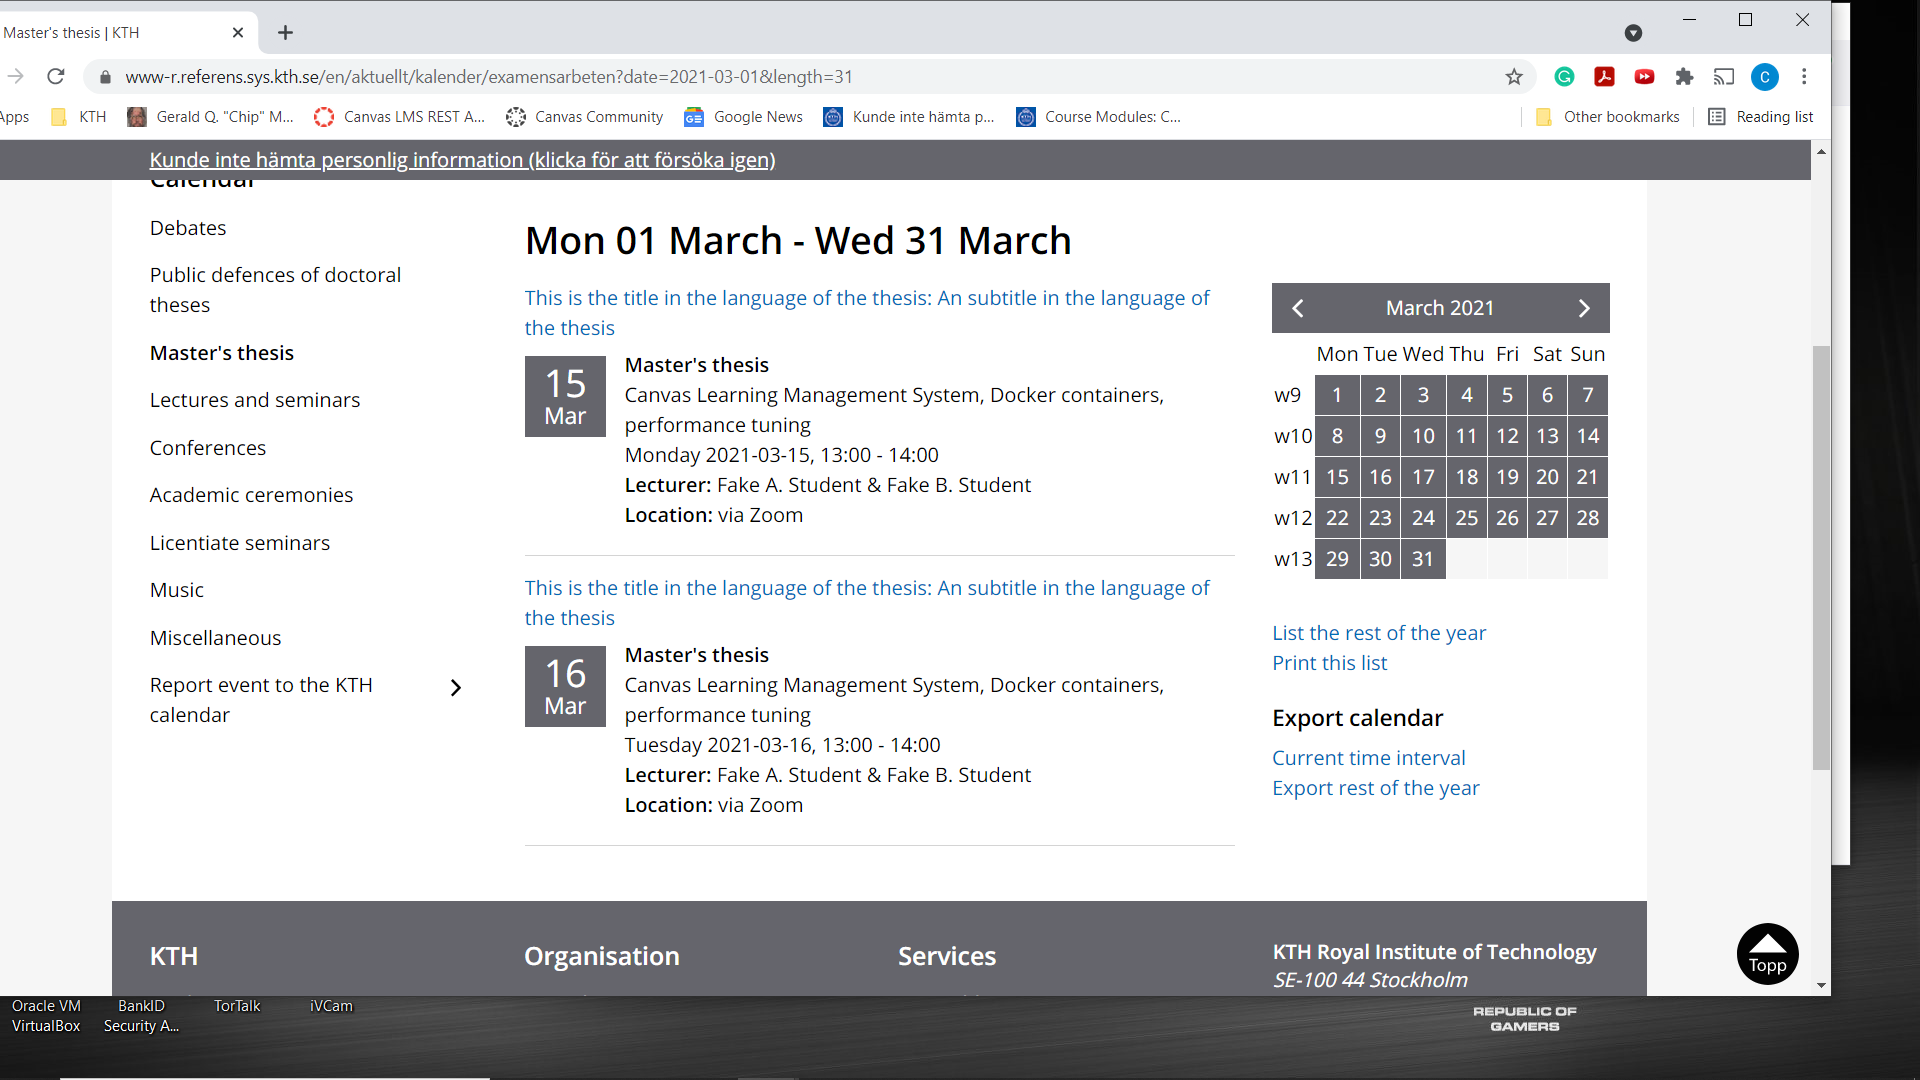
\includegraphics[width=0.99\textwidth, trim=3cm 2cm 8cm 0.2cm, clip]{README_notes/README-examiner-figures/cortina-2021-03-16-picture.png}}
  \end{center}
  \caption{KTH’s Cortina calendar showing two degree project events}
  \label{fig:cortinaPicture1}
\end{figure}
\FloatBarrier

\begin{figure}[!ht]
  \begin{center}
    \fbox{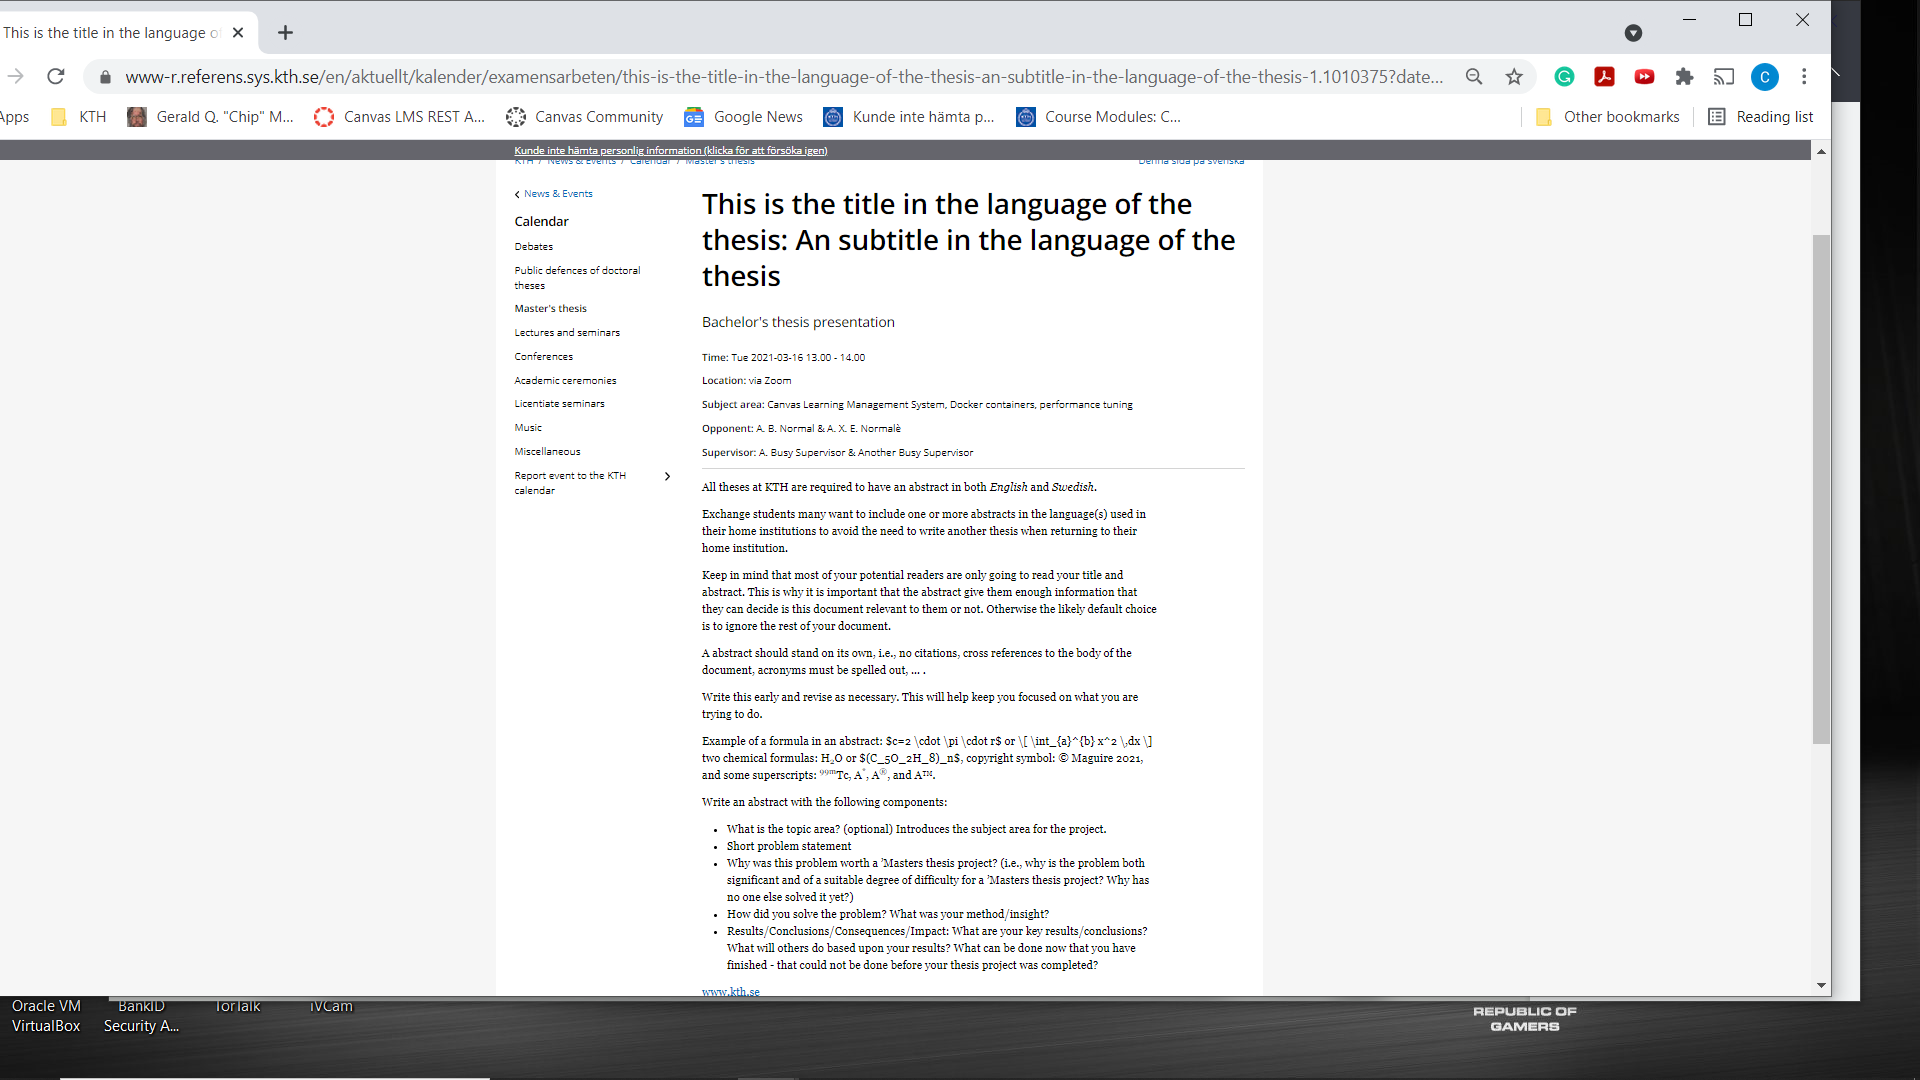
\includegraphics[width=1.0\textwidth, trim=3cm 2cm 16cm 0.2cm, clip]{README_notes/README-examiner-figures/cortina-2021-03-16-picture2.png}}
  \end{center}
  \caption{English version of the calendar}
  \label{fig:cortinaPicture2}
\end{figure}
\FloatBarrier	

\begin{figure}[!ht]
  \begin{center}
    \fbox{
\includegraphics[width=1.0\textwidth, trim=3cm 2cm 16cm 0.2cm, clip]{README_notes/README-examiner-figures/cortina-2021-03-16-picture3.png}}
  \end{center}
  \caption{Swedish version of the calendar}
  \label{fig:cortinaPicture3}
\end{figure}
\FloatBarrier

\Cref{lst:cortinaResponse} shows the response from doing a POST to the KTH Cortina API. Note that this is a prototype and as of the date of my experiments did not yet support having an examiner in a calendar event (hence I had to save and remove this element of the dict before passing the data to the API, then I restored this element for use by the subsequent routines).

\begin{lstlisting}[language={json}, caption={Response from the KTH Cortina API},label=lst:cortinaResponse]
{
  "advisor": "A. Busy Supervisor & Another Busy Supervisor",
  "contentId": "1.1010375",
  "contentName": {
    "en_GB": "This is the title in the language of the thesis: An subtitle in the language of the thesis",
    "sv_SE": "Detta är den svenska översättningen av titeln: Detta är den svenska översättningen av undertiteln"
  },
  "dates_endtime": "2021-03-16T13:00:00.000Z",
  "dates_starttime": "2021-03-16T12:00:00.000Z",
  "lead": {
    "en_GB": "Bachelor's thesis presentation",
    "sv_SE": "Kandidate Examensarbete presentation"
  },
  "lecturer": "Fake A. Student & Fake B. Student",
  "location": "via Zoom",
  "opponent": "A. B. Normal & A. X. E. Normalè",
  "organisation": {
    "school": "EECS",
    "department": "Datavetenskap"
  },
  "respondent": "",
  "respondentDepartment": "",
  "subjectarea": {
    "en_GB": "Canvas Learning Management System, Docker containers, performance tuning ",
    "sv_SE": "Canvas Lärplattform,Dockerbehållare, prestandajustering "
  },
  "seminartype": "thesis",
  "paragraphs_text": {
    "en_GB": "<p>All theses at KTH are required to have an abstract in both <i>English</i> and <i>Swedish</i>.</p> \n<p>Exchange students many want to include one or more abstracts in the language(s) used in their home institutions to avoid the need to write another thesis when returning to their home institution.</p> \n<p>Keep in mind that most of your potential readers are only going to read your title and abstract. This is why it is important that the abstract give them enough information that they can decide is this document relevant to them or not. Otherwise the likely default choice is to ignore the rest of your document.</p> \n<p>A abstract should stand on its own, i.e., no citations, cross references to the body of the document, acronyms must be spelled out, … .</p> \n<p>Write this early and revise as necessary. This will help keep you focused on what you are trying to do.</p> \n<p>Example of a formula in an abstract: $c=2 \\cdot \\pi \\cdot r$ or \\[ \\int_{a}^{b} x^2 \\,dx \\] two chemical formulas: H<sub>2</sub>O or $(C_5O_2H_8)_n$, copyright symbol: © Maguire 2021, and some superscripts: <sup>99m</sup>Tc, A<sup>*</sup>, A<sup>®</sup>, and A™.</p> \n<p>Write an abstract with the following components: </p> \n<ul> \n <li> What is the topic area? (optional) Introduces the subject area for the project. </li> \n <li> Short problem statement </li> \n <li> Why was this problem worth a ’Masters thesis project? (i.e., why is the problem both significant and of a suitable degree of difficulty for a ’Masters thesis project? Why has no one else solved it yet?) </li> \n <li> How did you solve the problem? What was your method/insight? </li> \n <li> Results/Conclusions/Consequences/Impact: What are your key results/conclusions? What will others do based upon your results? What can be done now that you have finished - that could not be done before your thesis project was completed?</li> \n</ul>\n",
    "sv_SE": "<p>Alla avhandlingar vid KTH måste ha ett abstrakt på både engelska och svenska.</p> \n<p>If you are writing your thesis in English, you can leave this until the final version. If you are writing your thesis in Swedish then this should be done first – and you should revise as necessary along the way.</p> \n<p>If you are writing your thesis in English, then this section can be a summary targeted at a more general reader. However, if you are writing your thesis in Swedish, then the reverse is true – your abstract should be for your target audience, while an English summary can be written targeted at a more general audience.</p> \n<p>This means that the English abstract and Swedish sammnfattning or Swedish abstract and English summary need not be literal translations of each other.</p> \n<p>The abstract in the language used for the thesis should be the first abstract, while the Summary/Sammanfattning in the other language can follow.</p>\n"
  },
  "uri": "https://www.kth.se"
}
\end{lstlisting}


\section{Actual example}
This example appears with the student’s permission. \Cref{fig:actualAnnouncementTop} shows the announcement for a 2\textsuperscript{nd} cycle thesis presentation in a Canvas course while \Cref{fig:actualAnnouncementBottom} shows the bottom part of the announcement. \Cref{fig:actualCalendarOpenned} shows the opened Canvas course calendar entry while \Cref{fig:actualEnglishAndSwedish} shows the Cortina calendar entry. Note that the Cortina calendar entry is in the development system and not the production calendar. \Cref{lst:extractPseudoAndJSONtoCalendar} shows the command to extract the JSON information from the student’s PDF file and then the command to make the announcement and calendar entries. \Cref{lst:extractedPseudoAndJSONtoCalendar} shows the extracted JSON.

Note that the entry was made on 2021-06-17, but the event was earlier. This entry was made with the new (as of this date) KTH Cortina Calendar API that supports the examiner and language of presentation fields. Additionally, it returns a canonicalUrl (the URL to this calendar entry). The program was extended to add this URL to the course announcement and course calendar entry.

\begin{figure}[!ht]
  \begin{center}
    \fbox{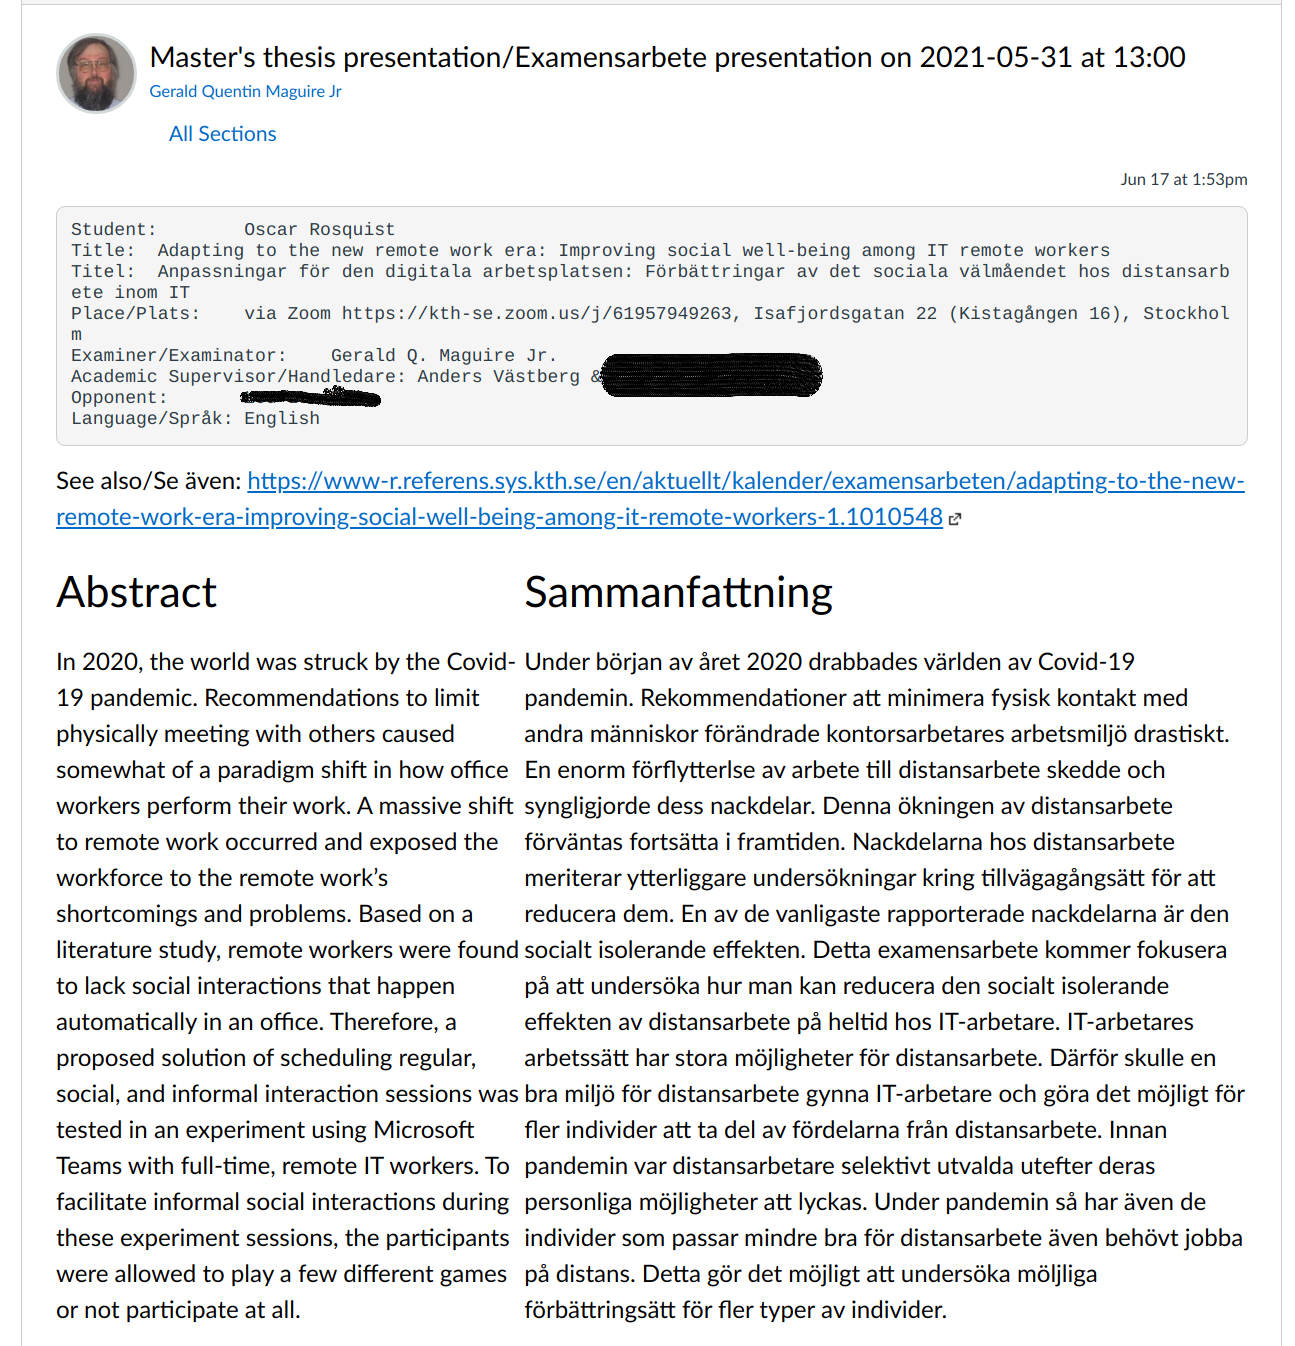
\includegraphics[width=1.2\textwidth]{README_notes/README-examiner-figures/Oscar-1-Screenshot_20210617_140037.png}}
  \end{center}
  \caption{Actual example of announcement in Canvas (top)}
  \label{fig:actualAnnouncementTop}
\end{figure}
\FloatBarrier

\begin{figure}[!ht]
  \begin{center}
    \fbox{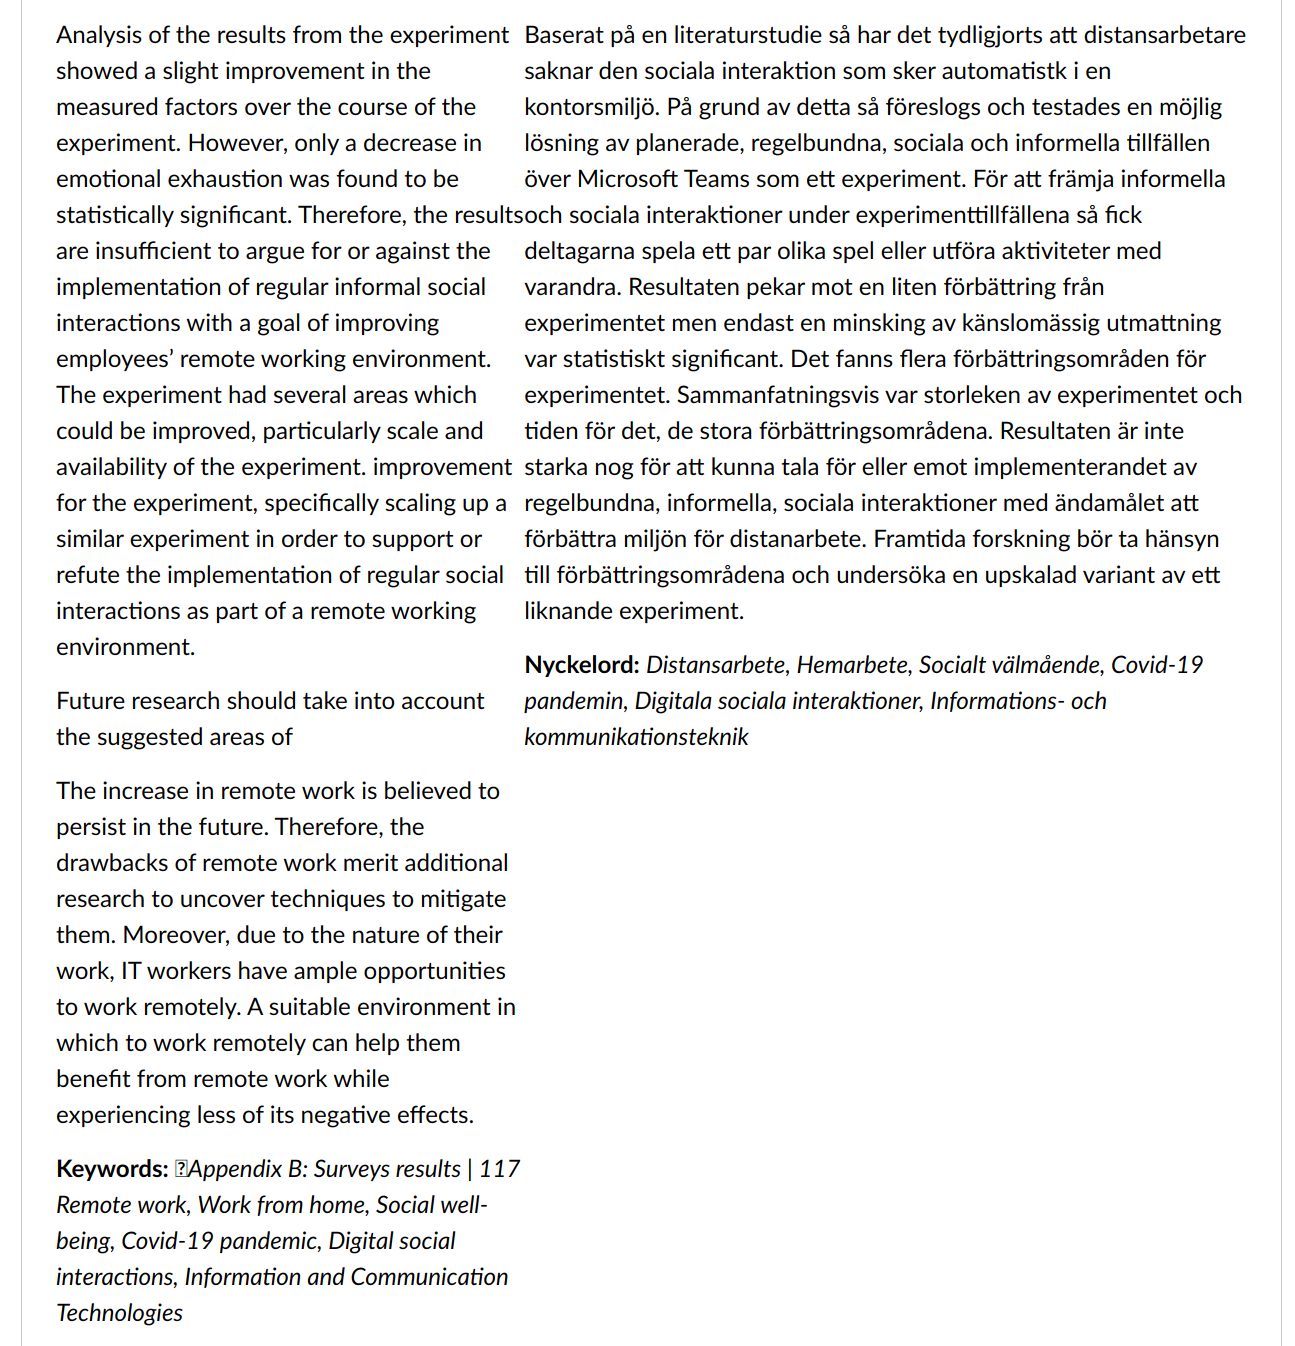
\includegraphics[width=1.2\textwidth]{README_notes/README-examiner-figures/Oscar-2-Screenshot_20210617_140116.png}}
  \end{center}
  \caption{Bottom of the announcement}
  \label{fig:actualAnnouncementBottom}
\end{figure}
\FloatBarrier
	
\begin{figure}[!ht]
  \begin{center}
    \fbox{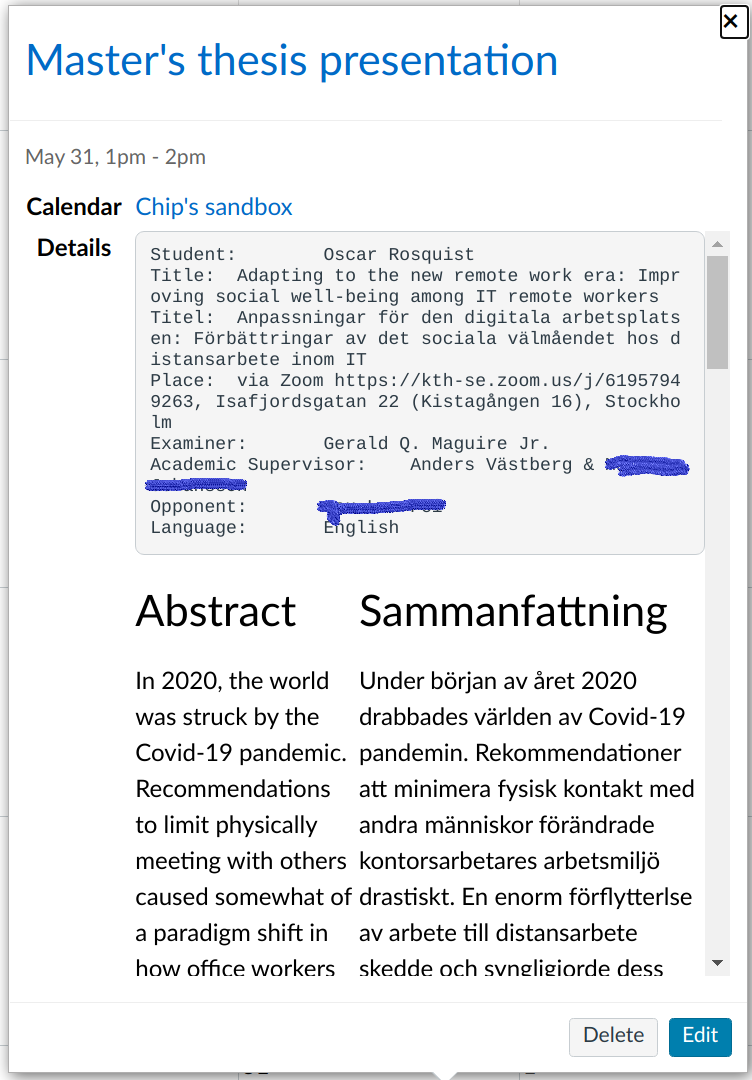
\includegraphics[width=1\textwidth]{README_notes/README-examiner-figures/oscar-course-calendar-Screenshot_20210617_143054.png}}
  \end{center}
  \caption{Opened version in course calendar}
  \label{fig:actualCalendarOpenned}
\end{figure}
\FloatBarrier	

\begin{figure}[!ht]
  \begin{center}
  \begin{subfigure}{0.45\textwidth}
    \fbox{
\includegraphics[width=\textwidth]{README_notes/README-examiner-figures/oscar-english-cortina.png}}
    \caption{English}
   \end{subfigure}
   \begin{subfigure}{0.45\textwidth}
    \fbox{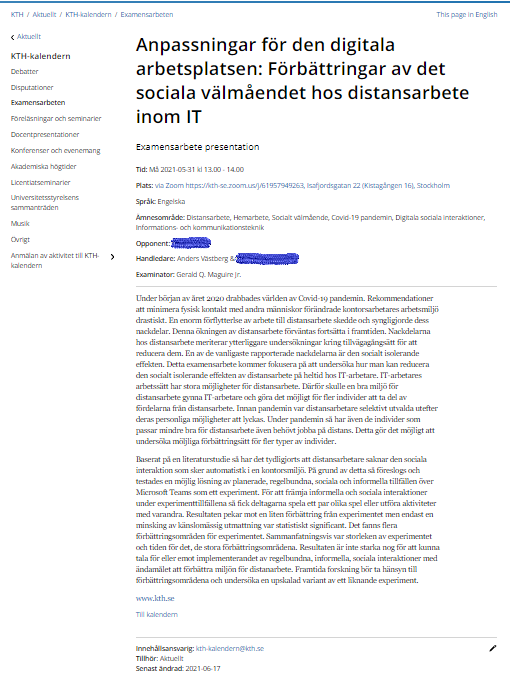
\includegraphics[width=\textwidth]{README_notes/README-examiner-figures/oscar-swedish-cortina.png}}
    \caption{Swedish}
  \end{subfigure}
  \end{center}
  \caption{The English (left) and Swedish (right) in the Cortina calendar}
  \label{fig:actualEnglishAndSwedish}
\end{figure}
\newpage

\Needspace*{4\baselineskip}
\begin{lstlisting}[language={bash}, caption={Commands to extract the JSON and to make the calendar entries and announcements}, label=lst:extractPseudoAndJSONtoCalendar]
./extract_pseudo_JSON-from_PDF.py --pdf oscar.pdf --json oscar.json
./JSON_to_calendar.py -c 11 --config config-test.json --json oscar.json
\end{lstlisting}

\begin{lstlisting}[language={json}, caption={Extracted JSON file oscar.json - edited for appearance here}, label=lst:extractedPseudoAndJSONtoCalendar]
{"Author1": {"Last name": "Rosquist", "First name": "Oscar", "Local User Id": "u1tmg8l6", "E-mail": "oscarros@kth.se", "organisation": {"L1": "School of Electrical Engineering and Computer Science "}}, "Degree": {"Educational program": "Degree Programme in Computer Science and Engineering"},
"Title": {"Main title": "Adapting to the new remote work era", "Subtitle": "Improving social well-being among IT remote workers", "Language": "eng"},
"Alternative title": {"Main title": "Anpassningar för den digitala arbetsplatsen", "Subtitle": "Förbättringar av det sociala välmåendet hos distansarbete inom IT", "Language": "swe"},
"Supervisor1": {"Last name": "Västberg", "First name": "Anders", "Local User Id": "u1ft3a12", "E-mail": "vastberg@kth.se", "organisation": {"L1": "School of Electrical Engineering and Computer Science ", "L2": "Computer Science"}},
"Supervisor2": {"Last name": "XXXXX", "First name": "XXXXX", "E-mail": "XXXXXX", "Other organisation": "XXXXX"},
"Examiner1": {"Last name": "Maguire Jr.", "First name": "Gerald Q.", "Local User Id": "u1d13i2c", "E-mail": "maguire@kth.se", "organisation": {"L1": "School of Electrical Engineering and Computer Science ", "L2": "Computer Science"}},
"Cooperation": {"Partner_name": "XXXXX"},
"Other information": {"Year": "2021", "Number of pages": "xvii,115"},
"Opponents": {"Name": "XXXXXX"}, "Presentation": {"Date": "2021-05-31 13:00", "Language": "eng", "Room": "via Zoom https://kth-se.zoom.us/j/61957949263", "Address": "Isafjordsgatan 22 (Kistagången 16)", "City": "Stockholm",
"National Subject Categories": "10201, 10206"}, "Number of lang instances": "2", "abstracts": {"eng": "<p>In 2020, the world was struck by the Covid-19 pandemic. …negative effects.</p>",
"swe": "<p>Under början av året 2020 drabbades världen av Covid-19 pandemin. … ett liknande experiment.</p>"},
"keywords": {"eng": "\n\fAppendix B: Surveys results | 117\n\nRemote work, Work from home, Social well-being, Covid-19 pandemic, Digital social interactions, Information and Communication\nTechnologies ",
"swe": "Distansarbete, Hemarbete, Socialt välmående, Covid-19 pandemin, Digitala sociala interaktioner, Informations- och kommunikationsteknik\n"}}	
\end{lstlisting}


\section{Change in how to enter the abstracts in \LaTeX}
In order to deal with both Babel and Polyglossia and both bibtex and biblatex, I have changed how the abstracts should be entered. Basically the idea is to insert a \textbackslash babelpolyLangStart \{language\_name\}  before the start of the abstract and \textbackslash babelpolyLangStop after the end of the abstract. These commands hide the difference between using Babel or Polyglossia. Additionally, they avoid the problem of the Overleaf GUI being confused about matching beginning and ending statements. \Cref{lst:babel} and \Cref{lst:babelSecondExample} show examples of how to enter an abstract and keywords while \Cref{lst:babelCMDS} shows the definition of the two commands.

Note that both Babel and Polyglossia expand the \textbackslash abstractname into the correct version of the name for an abstract in the current language. Unfortunately, neither package has an equivalent to provide the language specific version of “keywords”, so these have to be provided by the person entering the keywords. For example writing \textbackslash subsection*\{Nyckelord\} to have the Swedish word for keywords set as the subsection heading.

\begin{lstlisting}[language={[LaTeX]TeX}, caption={Example of the revised format for entering an abstract}, label=lst:babel]
\babelpolyLangStart{swedish}
\begin{abstract}
    \markboth{\abstractname}{}
\begin{scontents}[store-env=lang]
swe
\end{scontents}
\begin{scontents}[store-env=abstracts,print-env=true]
Alla avhandlingar vid KTH måste ha ett abstrakt på både engelska och svenska.

Om du skriver din avhandling på svenska ska detta göras först (och placera det som det första abstraktet) - och du bör revidera det vid behov.

If you are writing your thesis in English, you can leave this until the draft version that goes to your opponent for the written opposition. In this way you can provide the English and Swedish abstract/summary information that can be used in the announcement for your oral presentation.

If you are writing your thesis in English, then this section can be a summary targeted at a more general reader. However, if you are writing your thesis in Swedish, then the reverse is true – your abstract should be for your target audience, while an English summary can be written targeted at a more general audience.

This means that the English abstract and \foreignlanguage{swedish}{sammnfattning} 
or Swedish abstract and English summary need not be literal translations of each other.

The abstract in the language used for the thesis should be the first abstract, while the Summary/Sammanfattning in the other language can follow.
\end{scontents}
\subsection*{Nyckelord}
\begin{scontents}[store-env=keywords,print-env=true]
Canvas Lärplattform,Dockerbehållare, prestandajustering
\end{scontents}
\end{abstract}
\babelpolyLangStop{swedish}
\end{lstlisting}
	

\begin{lstlisting}[language={[LaTeX]TeX}, caption={Second example of the revised format for entering an abstract}, label=lst:babelSecondExample]
\generalExpl{Use the relevant language for abstracts for your home university.\\
Note that you may need to augment the set of language used in polyglossia or
babel (see the file kththesis.cls). The following languages include those languages that were used in theses at KTH in 2018-2019, except for one in Chinese.\\
Remove those versions that you do not need.\\
If adding a new language, when specifying the language for the abstract use the three-letter ISO 639-2 Code – specifically the "B" (bibliographic) variant of these codes (note that this is the same language code used in DiVA).
\babelpolyLangStart{french}
\begin{abstract}
    \markboth{\abstractname}{}
\begin{scontents}[store-env=lang]
fre
\end{scontents}
\begin{scontents}[store-env=abstracts,print-env=true]
Résumé en français.
\end{scontents}
\subsection*{Mots clés}
\begin{scontents}[store-env=keywords,print-env=true]
5-6 mots-clés
\end{scontents}
\end{abstract}
\babelpolyLangStop{french}
\cleardoublepage
\end{lstlisting}
\Needspace*{12\baselineskip}
\begin{lstlisting}[language={[LaTeX]TeX}, caption={The two commands used to help enter the language specification}, label=lst:babelCMDS]
\ifxeorlua
    \newcommand{\babelpolyLangStop}[1]{\end{#1}}
\else
    \newcommand{\babelpolyLangStop}[1]{\end{otherlanguage}}
\fi

\ifxeorlua
   \newcommand{\babelpolyLangStart}[1]{\begin{#1}}
\else
    \newcommand{\babelpolyLangStart}[1]{\begin{otherlanguage}{#1}}
\fi
\end{lstlisting}


\section{Adding keywords and PDF metadata}
\label{sec:addingKeywordsAndMetaDataToPDF}
In an effort to add the PDF metadata via the \texttt{hyperref} package, I also decided to add the keywords part of the PDF metadata. However, in order to do this I had to have the keywords \textit{before} the \textbackslash begin\{document\} command in the \LaTeX~file. To do so, I added three new commands to the \texttt{kththesis.cls} file, as shown in \Cref{lst:keywords}. The commands are used in the \texttt{examplethesis.tex} file to set up the keywords in both English and Swedish as well as include a new set of \LaTeX~commands to store the PDF metadata (as shown in \Cref{lst:storingkeywords}) using a file called \texttt{lib/pdf\_related\_includes.tex} (shown in \Cref{lst:informationforPDFfile}). Later the keywords that have been stored are inserted into the \LaTeX~after their respective language abstracts as shown in \Cref{lst:keywordsSection} and \Cref{lst:keywordsSectionSwedish}. The title page of the thesis and the PDF metadata are shown in \Cref{fig:pdfMetadata}. Note that both the English and Swedish version of the keywords are included in the metadata. Finally, the keywords appear (as expected) in the For DiVA data at the end of the PDF file as shown in \Cref{lst:keywordsFromForDIVA}.

Note that \textbackslash makeatletter and \textbackslash makeatother are use to include the character “@” as a letter and then return “@” to being a punctuation code. This use of “@” protects the internal names from being accessed outside of these two commands. More explicitly, \textbackslash EnglishKeywords is a function that takes one argument, the text of the English keywords, and then stores them into “@EnglishKeywords”. Later the text can be retrieved with the command \textbackslash InsertKeywords\{english\} or \textbackslash InsertKeywords\{swedish\}.
\Needspace*{15\baselineskip}
\begin{lstlisting}[language={[LaTeX]TeX}, caption={New commands in kththesis.cls}, label=lst:keywords]
% Keywords
\let\@EnglishKeywords\@empty
\newcommand{\EnglishKeywords}[1]{\def\@EnglishKeywords{#1}}

\let\@SwedishKeywords\@empty
\newcommand{\SwedishKeywords}[1]{\def\@SwedishKeywords{#1}}

\makeatletter
\newcommand{\InsertKeywords}[1]{
    \IfEqCase{#1}{%
    {english}{\@EnglishKeywords}
    {swedish}{\@SwedishKeywords}
  }[\typeout{argument must be english or swedish}]
}
\end{lstlisting}

\Cref{lst:storingkeywords} shows the storing of the keywords using the above commands and the include of the library to set up the PDF metadata.
\Needspace*{10\baselineskip}
\begin{lstlisting}[language={[LaTeX]TeX}, caption={shows the storing of the keywords using the above commands and the include of the library to set up the PDF meta data}, label=lst:storingkeywords]
% Enter the English and Swedish keywords here for use in the PDF meta data _and_ for later use
% following the respective abstract.
% Try to put the words in the same order in both to facilitate matching.
\EnglishKeywords{Canvas Learning Management System, Docker containers, performance tuning}
\SwedishKeywords{Canvas Lärplattform, Dockerbehållare, prestandajustering}

% Put the title, author, and keyword information into the PDF meta information
% This file contains the LaTeX to add information to the PDF file (specifically, author(s), title(s), and keywords
% It uses the hyperref package and should be included before the \begin{document}
%
% I want to acknowledge the inspiration of Karl Voit's template for TU Graz that inspired me to add the PDF document information
% For more information about his template see https://github.com/novoid/LaTeX-KOMA-template
% Note that this template does not use anything from his template other than the names of the information for the PDF meta fields, i.e., mytitle, myauthor, and mykeywords together with the idea of defining the corresponding newcommand to set the relevant hyperref parameters.

\makeatletter
\ifx\@subtitle\@empty
    \newcommand{\mytitle}{\@title}
\else
    \ifinswedish
        \newcommand{\mytitle}{\@title\xspace–\xspace\@subtitle}
    \else
        \newcommand{\mytitle}{\@title: \@subtitle}
    \fi
\fi
\makeatother

% Put the alternative title (and subtitle) into the PDF Subject meta
\makeatletter
\ifx\@altsubtitle\@empty\relax
    \newcommand{\myalttitle}{\@alttitle}
\else
    \ifinswedish
        \newcommand{\myalttitle}{\@alttitle: \@altsubtitle}
    \else
    \newcommand{\myalttitle}{\@alttitle\xspace–\xspace\@altsubtitle}
    \fi
    
\fi
\makeatother
\hypersetup{
     pdfsubject={\myalttitle}        % Subject field
}

\ifinswedish
\XMPLangAlt{en}{pdfsubject={\myalttitle}}
\else
\XMPLangAlt{sv}{pdfsubject={\myalttitle}}
\fi


\ifinswedish
\hypersetup{%
    pdflang={sv},
    pdfmetalang={sv},
    pdftitle={\mytitle}        % Title field
}
\XMPLangAlt{en}{pdftitle={\myalttitle}}
\else
\hypersetup{%
    pdflang={en},
    pdfmetalang={en},
    pdftitle={\mytitle}        % Title field
}
\XMPLangAlt{sv}{pdftitle={\myalttitle}}
\fi

\makeatletter
\ltx@ifpackageloaded{hyperxmp}{
\ifx\@secondAuthorsLastname\@empty
% Note that \hyxmp@comma is used explicitly rather than \xmpcomma
% As the later will simply turn into a comma in this context.
\StrSubstitute{\@authorsLastname}{,}{\hyxmp@comma}[\@authorsLastnameXMP]
    \newcommand{\myauthor}{\xmpquote{\@authorsFirstname\space\@authorsLastnameXMP}} 
\else
% Note that \hyxmp@comma is used explicitly rather than \xmpcomma
% As the later will simply turn into a comma in this context.
\StrSubstitute{\@authorsLastname}{,}{\hyxmp@comma}[\@authorsLastnameXMP]
\StrSubstitute{\@secondAuthorsLastname}{,}{\hyxmp@comma}[\@secondAuthorsLastnameXMP]
    \newcommand{\myauthor}{\xmpquote{\@authorsFirstname\space\@authorsLastnameXMP},
\xmpquote{\@secondAuthorsFirstname\space\@secondAuthorsLastnameXMP}}
\fi
}{
\ifx\@secondAuthorsLastname\@empty
    \newcommand{\myauthor}{\@authorsFirstname\space\@authorsLastname} 
\else
    \newcommand{\myauthor}{\@authorsFirstname\space\@authorsLastname,
\space\@secondAuthorsFirstname\space\@secondAuthorsLastname}
\fi
}% end of ifpackage conditional
\makeatother

\hypersetup{
     pdfauthor={\myauthor}      % Author field
}


\makeatletter
\ifx\@EnglishKeywords\@empty
    \ifx\@SwedishKeywords\@empty
        \newcommand{\mykeywords}{}
    \else
    \newcommand{\mykeywords}{\@SwedishKeywords}
    \fi
\else
    \ifx\@SwedishKeywords\@empty
        \newcommand{\mykeywords}{\@EnglishKeywords}
    \else
        \ifinswedish
            \newcommand{\mykeywords}{\@SwedishKeywords, \@EnglishKeywords}
        \else
            \newcommand{\mykeywords}{\@EnglishKeywords, \@SwedishKeywords}
        \fi
    \fi
\fi
\makeatother

\hypersetup{
     pdfkeywords={\mykeywords}        % Keywords field
}        
% I have _not_ set the following fields:
%    pdfcreator             % Creator field
%    pdfproducer            % Producer field

%% Note that the copyright information is added to the PDF file inside bookinfo{}
%% as until then, the copyright information is unknown.

% Put the alternative title (and subtitle) into the PDF Subject meta
\makeatletter
\ifx\@secondkthid\@empty\relax
    \newcommand{\mykthids}{author: \@kthid}
\else
    \newcommand{\mykthids}{author: \@kthid,\xspace
    secondauthor: \@secondkthid}
\fi
\makeatother

\hypersetup{
     pdfcontactemail={\mykthids}        % Subject field
}

% Add the TRITA number to the metadata
% Get and store information about the series and the number within this series, i.e, TRITA numbers
%"Series": \{
%	"Title of series": "TRITA-ICT-EX"
%	"No. in series": "2019:00"
\makeatletter
\ifinswedish
\hypersetup{
        pdfvolumenum={\@thesisSeries},        % put the series in the volume field
        pdfissuenum={\@thesisSeriesNumber},
        pdfpublisher={Kungliga Tekniska högskolan (KTH)},
        pdfpubtype={report}
}
\else
\hypersetup{
        pdfvolumenum={\@thesisSeries},        % put the series in the volume field
        pdfissuenum={\@thesisSeriesNumber},
        pdfpublisher={KTH Royal Institute of Technology},
        pdfpubtype={report}
}
\fi
\makeatother


% summary
\end{lstlisting}


The \texttt{lib/pdf\_related\_includes.tex} file contains the \LaTeX~to add information
to the PDF file (specifically, author(s), title(s), and keywords. It uses the
\texttt{hyperref} package and should be included before the \textbackslash begin{document}.
I want to acknowledge the inspiration of Karl Voit's template for TU Graz that inspired me to add the PDF document information. For more information about his template see \url{https://github.com/novoid/LaTeX-KOMA-template}
Note that my template does not use anything from his template other than the names of the information for the PDF meta fields, \ie \texttt{mytitle}, \texttt{myauthor}, and \texttt{mykeywords} together with the idea of defining the corresponding \texttt{newcommand} to set the relevant \texttt{hyperref} parameters. A result of both these decisions is that these command names are visible to the rest of the \LaTeX~file. See \Cref{lst:informationforPDFfile} for the code.

In keeping with the Swedish standard (Svenska skrivregler [Språkrådet 1.6.3 och 12.11.5]) a ``mellanslag tankstreck'' with a space before and after, \ie `` – '' is used to separate the title and subtitle when in Swedish this leads to a condition based on whether the document is in Swedish or not in the computation of \texttt{mytitle} and \texttt{myalttitle}.

As a result of adding support for the PDF metadata for copyright notice, the template now uses the \texttt{hyperxmp}. Because of this, if the author's name includes a suffix such as ``, Jr.'' or `` Jr.'', \ie the suffix can be separated with a comma or not as the author prefers to write their name; thus, there was a need to change the processing of \texttt{pdfauthor} information, as \texttt{hyperxmp} treats comma-separated strings in the author or keywords fields as being a list and converts these into a sequence of data in the metadata. This change is shown in \Cref{lst:informationforPDFfile} where the \textbackslash hyxmp@comma macro is used to insert something that is later replaced by a comma but is not treated as a comma when processing the \texttt{pdfauthor} information. The command \textbackslash xmpquote is used to wrap the whole name.
%\clearpage
\begin{lstlisting}[language={[LaTeX]TeX}, caption={lib/pdf\_related\_includes.tex
    (edited for readability and to avoid problems when rendering)}, columns=fullflexible, showstringspaces=false, label=lst:informationforPDFfile]
\makeatletter
\ifx\@subtitle\@empty
    \newcommand{\mytitle}{\@title}
\else
    \ifinswedish
        \newcommand{\mytitle}{\@title\xspace – \xspace\@subtitle}
    \else
        \newcommand{\mytitle}{\@title: \@subtitle}
    \fi
\fi
\makeatother

\makeatletter
\ltx@ifpackageloaded{hyperxmp}{
\ifx\@secondAuthorsLastname\@empty
% Note that \hyxmp@comma is used explicitly rather than \xmpcomma
% As the latter will simply turn into a comma in this context.
\StrSubstitute{\@authorsLastname}{,}{\hyxmp@comma}[\@authorsLastname]
    \newcommand{\myauthor}{\xmpquote{\@authorsFirstname\space\@authorsLastname}} 
\else
% Note that \hyxmp@comma is used explicitly rather than \xmpcomma
% As the latter will simply turn into a comma in this context.
\StrSubstitute{\@authorsLastname}{,}{\hyxmp@comma}[\@authorsLastname]
\StrSubstitute{\@secondAuthorsLastname}{,}{\hyxmp@comma}[\@secondAuthorsLastname]
    \newcommand{\myauthor}{\xmpquote{\@authorsFirstname\space\@authorsLastname},
\xmpquote{\@secondAuthorsFirstname\space\@secondAuthorsLastname}}
\fi
}{
\ifx\@secondAuthorsLastname\@empty
    \newcommand{\myauthor}{\@authorsFirstname\space\@authorsLastname} 
\else
    \newcommand{\myauthor}{\@authorsFirstname\space\@authorsLastname,
\space\@secondAuthorsFirstname\space\@secondAuthorsLastname}
\fi
}% end of ifpackage conditional
\makeatother

\hypersetup{
     pdfauthor={\myauthor}      % Author field
}dfauthor={\myauthor}      % Author field
}

% Put the alternative title (and subtitle) into the PDF Subject meta
\ifx\@altsubtitle\@empty\relax
    \newcommand{\myalttitle}{\@alttitle}
\else
    \ifinswedish
        \newcommand{\myalttitle}{\@alttitle: \@altsubtitle}
    \else
    \newcommand{\myalttitle}{\@alttitle\xspace – \xspace\@altsubtitle}
    \fi
    
\fi

\hypersetup{
     pdfsubject={\myalttitle}        % Subject field
}

\ifx\@EnglishKeywords\@empty
    \ifx\@SwedishKeywords\@empty
        \newcommand{\mykeywords}{}
    \else
    \newcommand{\mykeywords}{\@SwedishKeywords}
    \fi
\else
    \ifx\@SwedishKeywords\@empty
        \newcommand{\mykeywords}{\@EnglishKeywords}
    \else
        \ifinswedish
            \newcommand{\mykeywords}{\@SwedishKeywords, \@EnglishKeywords}
        \else
            \newcommand{\mykeywords}{\@EnglishKeywords, \@SwedishKeywords}
        \fi
    \fi
\fi
\makeatother

\hypersetup{
     pdfkeywords={\mykeywords}        % Keywords field
}        
\end{lstlisting}
\clearpage
\begin{lstlisting}[language={[LaTeX]TeX}, caption={Including the English language keywords below the English abstract}, label=lst:keywordsSection]
\subsection*{Keywords}
\begin{scontents}[store-env=keywords,print-env=true]
% If you set the EnglishKeywords earlier, you can retrieve them with:
% Alternative 1:
%\makeatletter
%\@EnglishKeywords
%\makeatother
%
% Alternative 2:
\InsertKeywords{english}
% If you did not set the EnglishKeywords earlier then simply enter the keywords here:
% Alternative 3:
% comma separate keywords, such as: Canvas Learning Management System, Docker containers, performance tuning
\end{scontents}
\end{lstlisting}

\begin{lstlisting}[language={[LaTeX]TeX}, caption={Including the Swedish language keywords below the Swedish abstract}, label=lst:keywordsSectionSwedish]
\subsection*{Nyckelord}
\begin{scontents}[store-env=keywords,print-env=true]
% SwedishKeywords were set earlier, hence we can use alternative 2
\InsertKeywords{swedish}
\end{scontents}
\end{abstract}
\end{lstlisting}



\begin{figure}[!ht]
  \begin{center}
    \fbox{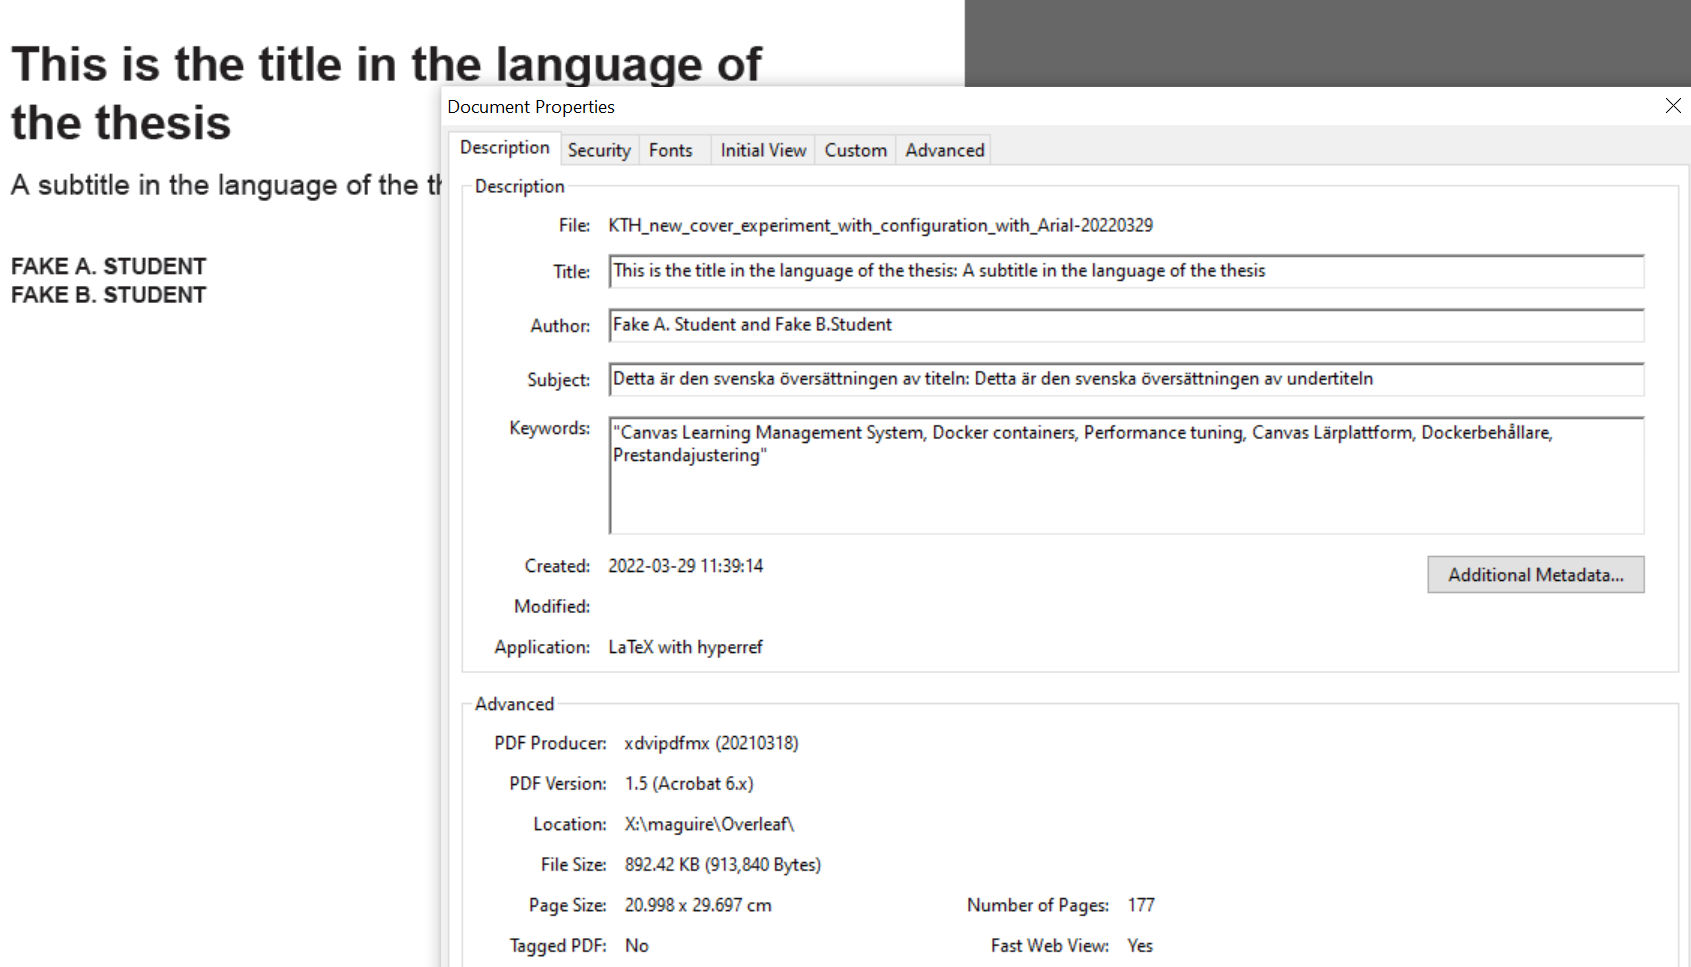
\includegraphics[width=1\textwidth]{README_notes/README-examiner-figures/PDF-file-metadata-Screenshot_20220330_085854.png}}
  \end{center}
  \caption{The title page of the thesis and the PDF metadata}
  \label{fig:pdfMetadata}
\end{figure}
\FloatBarrier	
\Needspace*{7\baselineskip}
\begin{lstlisting}[language={[LaTeX]TeX}, caption={The keywords appear as expected in the For DiVA data at the end of the PDF file}, label=lst:keywordsFromForDIVA]	
”Keywords[eng ]”: €€€€
Canvas Learning Management System, Docker containers, Performance tuning €€€€,

”Keywords[swe ]”: €€€€
Canvas Lärplattform, Dockerbehållare, Prestandajustering €€€€,
\end{lstlisting}

\section{Other variants of the JSON\_to\_calendar.py}
\label{sec:otherVariantsofJSONtoCalendar}
For testing purposes, I also created functionality in \texttt{JSON\_to\_calendar.py} to insert a fixed event (this was my first test) and to take as input a MODS file. The MODS file was created from a DiVA feed of theses presented in 2020 through to the 25\textsuperscript{th} of April. However, one limitation that I found is that other than myself, few people have been entering the date and time for the oral presentation. Unfortunately, since I wanted to test making calendar announcements, I needed data and time!

\Needspace*{2\baselineskip}
\textbf{NB}: I have assumed that each degree project presentation lasts one hour – since the KTH Cortina calendar API needs both a starting and ending time.

These other variants probably should not be kept, but rather the architecture should be similar to that shown in \Cref{fig:severalPossibleInputs}. Additionally, when taking data from other types of sources, one can take advantage of the data that is in a Canvas degree project course room to help when processing of the source data.

\begin{figure}[!ht]
\resizebox{\textwidth}{!}{%
\begin{tikzpicture}
[align=left,node distance=2cm]


\node (latexFile) [tape,tape bend top=none,draw,font=\sffamily] {\LaTeX file};
\node (PDFfile) [tape,tape bend top=none,draw,font=\sffamily, above of=latexFile] {PDF file};
\node (DOCXFile) [tape,tape bend top=none,draw,font=\sffamily, below of=latexFile] {DOCX file};

\node (extractor) [processBox, right=1cm of latexFile] {Extractor};
\node (jsonFile) [tape,tape bend top=none,draw,font=\sffamily, right=0.5cm of extractor] {JSON file};
\node (start) [processBox, right=0.5cm of jsonFile] {JSON\_to\_calendar};
\node (MODSFile) [tape,tape bend top=none,draw,font=\sffamily, above of=jsonFile] {MODS file};

\node (calendarEvent) [destinationBox, right=1cm of start] {Canvas calendar event};
\node (announcement) [destinationBox,  above of =calendarEvent] {Canvas announcement};
\node (cortinaCalendarEvent) [destinationBox,  right=0.5cm of start, below of=calendarEvent] {KTH Cortina calendar event};
\draw [arrow] (latexFile) --  (extractor.west);
\draw [arrow] (PDFfile) --  (extractor.west);
\draw [arrow] (DOCXFile) --  (extractor.west);
\draw [arrow] (extractor) --  (jsonFile.west);
\draw [arrow] (jsonFile) --  (start.west);
\draw [arrow] (start.east) --  (announcement.west);
\draw [arrow] (start.east) -- (calendarEvent);
\draw [arrow] (start.east) -- (cortinaCalendarEvent.west);
\draw [arrow, dashed] (MODSFile) --  node[right] {only for testing} (start.west);
\end{tikzpicture}
}
\caption{Several possible inputs to JSON\_to\_calendar.py  and its outputs}
  \label{fig:severalPossibleInputs}
\end{figure}




\section{JSON to MODS file}
\label{sec:JSONtoMODSfile}
In keeping with the idea of using the JSON file to drive other applications, the program JSON\_to\_MODS.py to creates a MODS file using the information from the arguments and a JSON file.
The program is patterned after the \texttt{JSON\_to\_calendar} and \texttt{JSON\_to\_cover} programs. The program outputs a MODS file called: \texttt{modsXML.xml}. The program is run as shown in \Cref{lst:jsonToMods}.
\Needspace*{5\baselineskip}
\begin{lstlisting}[language={bash}, caption={Example of using JSON\_to\_MODS.py}, label=lst:jsonToMods]
./JSON_to_MODS.py -c 11   --json test12.json --trita "TRITA-EECS-EX-2021:219" --testing
\end{lstlisting}


Note that currently the Canvas course information is not used. Note also that the “—testing” flag forces the report series to be  "TRITA-ICT-EX" overriding the actual series in in the input version of the DiVA data.

If acronyms are used in the abstracts, you can also add the “- -acronyms acronyms.tex” argument to the command line and the program will process the acronyms.

As noted above, you will get a file named \texttt{modsXML.xml} that you can manually import into DiVA. This process is shown in \Cref{sec:importingMODSfiletoDiVA}. I seem to be able to import these files into the test instance of DiVA:	\url{https://kth.test.diva-portal.org/dream/import/importList.jsf}. Another side-effect of the testing flag is to use the test instance of DiVA. \textbf{NB}: The organization units are different between the production and test version of DiVA. When run without the testing flag set, the MODS file can be imported into the production version of DiVA.

This program has been extended to be able to take the TRITA number information from the MODS file.


\subsection{Example of JSON to MODS}
The process of importing the MODS data into DiVA begins with the extracted JSON file (note that I have changed some of the formatting of the pseudo JSON information and added the export of the program code). An example of the JSON information is shown in \Cref{lst:test12.json}. The resulting MODS file is shown in \Cref{lst:test12.mods}.

\begin{lstlisting}[language={json}, caption={test12.json (manually reformatted)}, label=lst:test12.json]
{"Author1": {"Last name": "Student", "First name": "Fake A.", "Local User Id": "u100001", "E-mail": "a@kth.se", "organisation": {"L1": "School of Electrical Engineering and Computer Science "}}, 
"Author2": {"Last name": "Student", "First name": "Fake B.", "Local User Id": "u100002", "E-mail": "b@kth.se", "organisation": {"L1": "School of Architecture and the Built Environment "}}, 
"Degree": {"Educational program": "Bachelor’s Programme in Information and Communication Technology", "programcode": "TCOMK", "Level": "1", "Course code": "IA150X", "Credits": "15.0", "Exam": "Bachelors degree", "subjectArea": "Information and Communication Technology"},
"Title": {"Main title": "This is the title in the language of the thesis", "Subtitle": "An subtitle in the language of the thesis", "Language": "eng"},
"Alternative title": {"Main title": "Detta är den svenska översättningen av titeln", "Subtitle": "Detta är den svenska översättningen av undertiteln", "Language": "swe"},
"Supervisor1": {"Last name": "Supervisor", "First name": "A. Busy", "Local User Id": "u100003", "E-mail": "sa@kth.se", "organisation": {"L1": "School of Electrical Engineering and Computer Science ", "L2": "Computer Science"}},
"Supervisor2": {"Last name": "Supervisor", "First name": "Another Busy", "Local User Id": "u100003", "E-mail": "sb@kth.se", "organisation": {"L1": "School of Architecture and the Built Environment ", "L2": "Public Buildings"}}, 
"Supervisor3": {"Last name": "Supervisor", "First name": "Third Busy", "E-mail": "sc@tu.va", "Other organisation": "Timbuktu University, Department of Pseudoscience"},
"Examiner1": {"Last name": "Maguire Jr.", "First name": "Gerald Q.", "Local User Id": "u1d13i2c", "E-mail": "maguire@kth.se", "organisation": {"L1": "School of Electrical Engineering and Computer Science ", "L2": "Computer Science"}},
"Cooperation": {"Partner_name": "Företaget AB"}, "National Subject Categories": "10201, 10206", "Other information": {"Year": "2021", "Number of pages": "xxxiii,35"}, "Opponents": {"Name": "A. B. Normal & A. X. E. Normalè"}, "Presentation": {"Date": "2021-03-15 13:00", "Language": "eng", "Room": "via Zoom https://kth-se.zoom.us/j/ddddddddddd", "Address": "Isafjordsgatan 22 (Kistagången 16)", "City": "Stockholm"},
"Number of lang instances": "10", "abstracts": {"eng": "<p>All theses at KTH are <bold>required</bold> to have an abstract in both <i>English</i> and <i>Swedish</i>.</p><p>Exchange students many want to include one or more abstracts in the language(s) used in their home institutions to avoid the need to write another thesis when returning to their home institution.</p><p>Keep in mind that most of your potential readers are only going to read your <tt>title</tt> and <tt>abstract</tt>. This is why it is important that the abstract give them enough information that they can decide is this document relevant to them or not. Otherwise the likely default choice is to ignore the rest of your document.</p><p>A abstract should stand on its own, i.e., no citations, cross references to the body of the document, acronyms must be spelled out, … .</p><p>Write this early and revise as necessary. This will help keep you focused on what you are trying to do.</p><p>Write an abstract with the following components: </p><ul><li> What is the topic area? (optional) Introduces the subject area for the project. </li><li> Short problem statement </li><li> Why was this problem worth a Bachelor’s/’Masters thesis project? (i.e., why is the problem both significant and of a suitable degree of difficulty for a Bachelor’s/’Masters thesis project? Why has no one else solved it yet?) </li><li> How did you solve the problem? What was your method/insight? </li><li> Results/Conclusions/Consequences/Impact: What are your key results/conclusions? What will others do based upon your results? What can be done now that you have finished - that could not be done before your thesis project was completed?</li></ul><p>announcement of the oral presentation and for entering data into DiVA</p><p>\\pi \\cdot r$ or \\[ \\int_{a}^{b} x^2 \\,dx \\]</p><p></p><p> A<sup>*</sup>, A<sup>&reg;</sup>, and A&trade;.</p><p> first chemical formula can be handled, while the second will require hand editing</p>",
"swe": "<p>Alla avhandlingar vid KTH <bold>måste ha</bold> ett abstrakt på både <i>engelska</i> och <i>svenska</i>.</p><p>Om du skriver din avhandling på svenska ska detta göras först (och placera det som det första abstraktet) - och du bör revidera det vid behov.</p><p>If you are writing your thesis in English, you can leave this until the draft version that goes to your opponent for the written opposition. In this way you can provide the English and Swedish abstract/summary information that can be used in the announcement for your oral presentation.</p><p>If you are writing your thesis in English, then this section can be a summary targeted at a more general reader. However, if you are writing your thesis in Swedish, then the reverse is true – your abstract should be for your target audience, while an English summary can be written targeted at a more general audience.</p><p>This means that the English abstract and Swedish sammnfattning or Swedish abstract and English summary need not be literal translations of each other.</p><p>The abstract in the language used for the thesis should be the first abstract, while the Summary/Sammanfattning in the other language can follow.</p>",
"fre": "<p>Résumé en français.</p>", "spa": "<p>Résumé en espagnol.</p>", "ita": "<p>Sommario in italiano.</p>",
"nor": "<p>Sammendrag på norsk.</p>", "ger": "", "dan": "<p>Abstrakt på dansk.</p>",
"dut": "<p>Zusammenfassung in Deutsch.</p><p>Samenvatting in het Nederlands.</p><p>Eesti keeles kokkuvõte.</p>", "est": ""},
"keywords": {"eng": "Canvas Learning Management System, Docker containers, Performance tuning ",
"swe": "Canvas Lärplattform, Dockerbehållare, Prestandajustering\nNyckelord som beskriver innehållet i uppsatsrapporten\n",
"fre": "5-6 mots-clés ", "spa": "5-6 Palabras claves ", "ita": "5-6 parole chiave ",
"nor": "5-6 nøkkelord ", "ger": "5-6 Schlüsselwörter ", "dan": "5-6 Søgeord ",
"dut": "5-6 trefwoorden ", "est": "5-6 Märksõnad "}}
\end{lstlisting}

\clearpage

\begin{lstlisting}[language={XML}, caption={test12.mods (reformatted in EMACS using XML mode)}, label=lst:test12.mods]
<modsCollection xmlns="http://www.loc.gov/mods/v3" xmlns:xsi="http://www.w3.org/2001/XMLSchema-instance" xsi:schemaLocation="http://www.loc.gov/mods/v3 http://www.loc.gov/standards/mods/v3/mods-3-2.xsd">
  <mods xmlns="http://www.loc.gov/mods/v3" xmlns:xsi="http://www.w3.org/2001/XMLSchema-instance" xmlns:xlink="http://www.w3.org/1999/xlink" version="3.2" xsi:schemaLocation="http://www.loc.gov/mods/v3 http://www.loc.gov/standards/mods/v3/mods-3-2.xsd">
    <genre authority="diva" type="publicationTypeCode">studentThesis
    </genre>
    <genre authority="diva" type="publicationType" lang="swe">Studentuppsats (Examensarbete)
    </genre>
    <genre authority="diva" type="publicationType" lang="eng">Student thesis
    </genre>
    <genre authority="diva" type="publicationType" lang="nor">Oppgave
    </genre>
    <name type="personal" authority="kth" xlink:href="u100001">
      <namePart type="family">Student
      </namePart>
      <namePart type="given">Fake A.
      </namePart>
      <description>email=a@kth.se
      </description>
      <role>
	<roleTerm type="code" authority="marcrelator">aut
	</roleTerm>
      </role>
    </name>
    <name type="personal" authority="kth" xlink:href="u100002">
      <namePart type="family">Student
      </namePart>
      <namePart type="given">Fake B.
      </namePart>
      <description>email=b@kth.se
      </description>
      <role>
	<roleTerm type="code" authority="marcrelator">aut
	</roleTerm>
      </role>
    </name>
    <name type="personal" authority="kth" xlink:href="u1d13i2c">
      <namePart type="family">Maguire Jr.
      </namePart>
      <namePart type="given">Gerald Q.
      </namePart>
      <description>email=maguire@kth.se
      </description>
      <affiliation>KTH, School of Electrical Engineering and Computer Science, Computer Science
      </affiliation>
      <role>
	<roleTerm type="code" authority="marcrelator">mon
	</roleTerm>
      </role>
    </name>
    <name type="personal" authority="kth" xlink:href="u100003">
      <namePart type="family">Supervisor
      </namePart>
      <namePart type="given">A. Busy
      </namePart>
      <affiliation>School of Electrical Engineering and Computer Science, Computer Science
      </affiliation>
      <description>email=sa@kth.se
      </description>
      <role>
	<roleTerm type="code" authority="marcrelator">ths
	</roleTerm>
      </role>
    </name>
    <name type="personal" authority="kth" xlink:href="u100003">
      <namePart type="family">Supervisor
      </namePart>
      <namePart type="given">Another Busy
      </namePart>
      <affiliation>School of Architecture and the Built Environment, Public Buildings
      </affiliation>
      <description>email=sb@kth.se
      </description>
      <role>
	<roleTerm type="code" authority="marcrelator">ths
	</roleTerm>
      </role>
    </name>
    <name type="personal">
      <namePart type="family">Supervisor
      </namePart>
      <namePart type="given">Third Busy
      </namePart>
      <affiliation>Timbuktu University, Department of Pseudoscience
      </affiliation>
      <description>email=sc@tu.va
      </description>
      <role>
	<roleTerm type="code" authority="marcrelator">ths
	</roleTerm>
      </role>
    </name>
    <name>
      <namePart>KTH
      </namePart>
      <namePart> School of Electrical Engineering and Computer Science
      </namePart>
      <namePart> Computer Science
      </namePart>
      <role>
	<roleTerm type="code" authority="marcrelator">pbl
	</roleTerm>
      </role>
    </name>
    <titleInfo  lang="eng">
      <title>This is the title in the language of the thesis
      </title>
      <subTitle>An subtitle in the language of the thesis
      </subTitle>
    </titleInfo >
    <titleInfo  lang="swe" type="alternative">
      <title>Detta är den svenska översättningen av titeln
      </title>
      <subTitle>Detta är den svenska översättningen av undertiteln
      </subTitle>
    </titleInfo >
    <subject  lang="eng">
      <topic>Canvas Learning Management System
      </topic>
      <topic>Docker containers
      </topic>
      <topic>Performance tuning
      </topic>
    </subject >
    <subject  lang="swe">
      <topic>Canvas Lärplattform
      </topic>
      <topic>Dockerbehållare
      </topic>
      <topic>Prestandajustering Nyckelord som beskriver innehållet i uppsatsrapporten
      </topic>
    </subject >
    <subject  lang="fre">
      <topic>5-6 mots-clés
      </topic>
    </subject >
    <subject  lang="spa">
      <topic>5-6 Palabras claves
      </topic>
    </subject >
    <subject  lang="ita">
      <topic>5-6 parole chiave
      </topic>
    </subject >
    <subject  lang="nor">
      <topic>5-6 nøkkelord
      </topic>
    </subject >
    <subject  lang="ger">
      <topic>5-6 Schlüsselwörter
      </topic>
    </subject >
    <subject  lang="dan">
      <topic>5-6 Søgeord
      </topic>
    </subject >
    <subject  lang="dut">
      <topic>5-6 trefwoorden
      </topic>
    </subject >
    <subject  lang="est">
      <topic>5-6 Märksõnad
      </topic>
    </subject >
    <abstract  lang="eng">&lt;p&gt;All theses at KTH are &lt;bold&gt;required&lt;/bold&gt; to have an abstract in both &lt;i&gt;English&lt;/i&gt; and &lt;i&gt;Swedish&lt;/i&gt;.&lt;/p&gt;&lt;p&gt;Exchange students many want to include one or more abstracts in the language(s) used in their home institutions to avoid the need to write another thesis when returning to their home institution.&lt;/p&gt;&lt;p&gt;Keep in mind that most of your potential readers are only going to read your &lt;tt&gt;title&lt;/tt&gt; and &lt;tt&gt;abstract&lt;/tt&gt;. This is why it is important that the abstract give them enough information that they can decide is this document relevant to them or not. Otherwise the likely default choice is to ignore the rest of your document.&lt;/p&gt;&lt;p&gt;A abstract should stand on its own, i.e., no citations, cross references to the body of the document, acronyms must be spelled out, … .&lt;/p&gt;&lt;p&gt;Write this early and revise as necessary. This will help keep you focused on what you are trying to do.&lt;/p&gt;&lt;p&gt;Write an abstract with the following components: &lt;/p&gt;&lt;ul&gt;&lt;li&gt; What is the topic area? (optional) Introduces the subject area for the project. &lt;/li&gt;&lt;li&gt; Short problem statement &lt;/li&gt;&lt;li&gt; Why was this problem worth a Bachelor’s/’Masters thesis project? (i.e., why is the problem both significant and of a suitable degree of difficulty for a Bachelor’s/’Masters thesis project? Why has no one else solved it yet?) &lt;/li&gt;&lt;li&gt; How did you solve the problem? What was your method/insight? &lt;/li&gt;&lt;li&gt; Results/Conclusions/Consequences/Impact: What are your key results/conclusions? What will others do based upon your results? What can be done now that you have finished - that could not be done before your thesis project was completed?&lt;/li&gt;&lt;/ul&gt;&lt;p&gt;announcement of the oral presentation and for entering data into DiVA&lt;/p&gt;&lt;p&gt;\pi \cdot r$ or &lt;span class='math-tex'&gt;\[ \int_{a}^{b} x^2 \,dx \]&lt;/span&gt;&lt;/p&gt;&lt;p&gt;&lt;/p&gt;&lt;p&gt; A&lt;sup&gt;*&lt;/sup&gt;, A&lt;sup&gt;&amp;reg;&lt;/sup&gt;, and A&amp;trade;.&lt;/p&gt;&lt;p&gt; first chemical formula can be handled, while the second will require hand editing&lt;/p&gt;
    </abstract >
    <abstract  lang="swe">&lt;p&gt;Alla avhandlingar vid KTH &lt;bold&gt;måste ha&lt;/bold&gt; ett abstrakt på både &lt;i&gt;engelska&lt;/i&gt; och &lt;i&gt;svenska&lt;/i&gt;.&lt;/p&gt;&lt;p&gt;Om du skriver din avhandling på svenska ska detta göras först (och placera det som det första abstraktet) - och du bör revidera det vid behov.&lt;/p&gt;&lt;p&gt;If you are writing your thesis in English, you can leave this until the draft version that goes to your opponent for the written opposition. In this way you can provide the English and Swedish abstract/summary information that can be used in the announcement for your oral presentation.&lt;/p&gt;&lt;p&gt;If you are writing your thesis in English, then this section can be a summary targeted at a more general reader. However, if you are writing your thesis in Swedish, then the reverse is true – your abstract should be for your target audience, while an English summary can be written targeted at a more general audience.&lt;/p&gt;&lt;p&gt;This means that the English abstract and Swedish sammnfattning or Swedish abstract and English summary need not be literal translations of each other.&lt;/p&gt;&lt;p&gt;The abstract in the language used for the thesis should be the first abstract, while the Summary/Sammanfattning in the other language can follow.&lt;/p&gt;
    </abstract >
    <abstract  lang="fre">&lt;p&gt;Résumé en français.&lt;/p&gt;
    </abstract >
    <abstract  lang="spa">&lt;p&gt;Résumé en espagnol.&lt;/p&gt;
    </abstract >
    <abstract  lang="ita">&lt;p&gt;Sommario in italiano.&lt;/p&gt;
    </abstract >
    <abstract  lang="nor">&lt;p&gt;Sammendrag på norsk.&lt;/p&gt;
    </abstract >
    <abstract  lang="ger" />
    <abstract  lang="dan">&lt;p&gt;Abstrakt på dansk.&lt;/p&gt;
    </abstract >
    <abstract  lang="dut">&lt;p&gt;Zusammenfassung in Deutsch.&lt;/p&gt;&lt;p&gt;Samenvatting in het Nederlands.&lt;/p&gt;&lt;p&gt;Eesti keeles kokkuvõte.&lt;/p&gt;
    </abstract >
    <abstract  lang="est" />
    <physicalDescription>
      <form authority="marcform">electronic
      </form>
      <extent>xxxiii,35
      </extent>
    </physicalDescription>
    <originInfo>
      <place>
	<placeTerm>Stockholm
	</placeTerm>
      </place>
      <publisher>KTH Royal Institute of Technology
      </publisher>
      <dateIssued>2021
      </dateIssued>
      <dateOther type="defence">2021-03-15T13:00:00
      </dateOther>
    </originInfo>
    <typeOfResource>text
    </typeOfResource>
    <relatedItem  type="series">
      <titleInfo>
	<title>TRITA-ICT-EX
	</title>
	<identifier type="local">5952
	</identifier>
	<identifier type="issue number">2021:219
	</identifier>
      </titleInfo>
    </relatedItem >
    <note lang="swe" type="level">Självständigt arbete på grundnivå (kandidatexamen)
    </note>
    <note lang="eng" type="degree">Bachelors degree
    </note>
    <note lang="swe" type="universityCredits">10 poäng / 15 hp
    </note>
    <subject lang="swe" xlink:href="10329">
      <topic>Informations- och kommunikationsteknik
      </topic>
      <genre>Subject/course
      </genre>
    </subject>
    <subject lang="eng" xlink:href="10329">
      <topic>Information and Communication Technology
      </topic>
      <genre>Subject/course
      </genre>
    </subject>
    <subject lang="swe" xlink:href="9925">
      <topic>Teknologie kandidatexamen - Informations- och kommunikationsteknik
      </topic>
      <genre>Educational program
      </genre>
    </subject>
    <subject lang="eng" xlink:href="9925">
      <topic>Bachelor of Science - Information and Communication Technology
      </topic>
      <genre>Educational program
      </genre>
    </subject>
    <language objectPart="defence">
      <languageTerm type="code" authority="iso639-2b">eng
      </languageTerm>
    </language>
    <note type="venue">via Zoom https://kth-se.zoom.us/j/ddddddddddd,Isafjordsgatan 22 (Kistagången 16),Stockholm
    </note>
    <note type="cooperation">Företaget AB
    </note>
    <subject lang="eng" authority="hsv" xlink:href="10201">
      <topic>Natural Sciences
      </topic>
      <topic>Computer and Information Sciences
      </topic>
      <topic>Computer Sciences
      </topic>
    </subject>
    <subject lang="swe" authority="hsv" xlink:href="10201">
      <topic>Naturvetenskap
      </topic>
      <topic>Data- och informationsvetenskap
      </topic>
      <topic>Datavetenskap (datalogi)
      </topic>
    </subject>
    <subject lang="eng" authority="hsv" xlink:href="10206">
      <topic>Natural Sciences
      </topic>
      <topic>Computer and Information Sciences
      </topic>
      <topic>Computer Engineering
      </topic>
    </subject>
    <subject lang="swe" authority="hsv" xlink:href="10206">
      <topic>Naturvetenskap
      </topic>
      <topic>Data- och informationsvetenskap
      </topic>
      <topic>Datorteknik
      </topic>
    </subject>
  </mods>
</modsCollection>
\end{lstlisting}
	
\subsection{Importing MODS file to DiVA}
\label{sec:importingMODSfiletoDiVA}

\Cref{fig:divaImport1} to \Cref{fig:divaImport4} show the process of importing the MODS file into DiVA. Note that it skips the first user interface form (as this differs between users).

\begin{figure}[!ht]
  \begin{center}
    \fbox{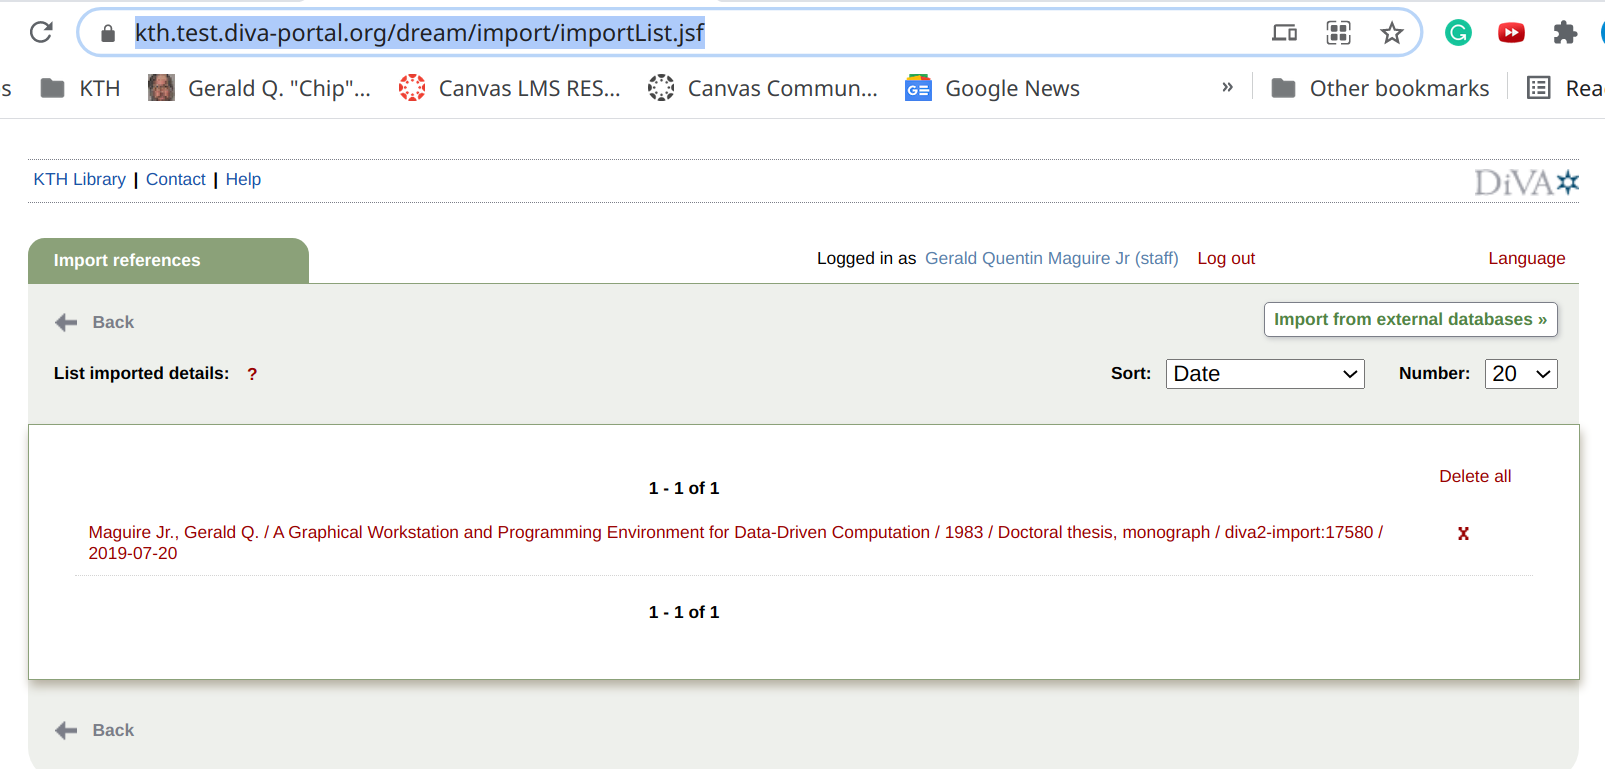
\includegraphics[width=1\textwidth]{README_notes/README-examiner-figures/import-1-Screenshot_20210626_234259.png}}
  \end{center}
  \caption[The import process – step 1]{The import process – step 1 – click on the “Import from external database” button on the upper right corner}
  \label{fig:divaImport1}
\end{figure}
\FloatBarrier

\begin{figure}[!ht]
  \begin{center}
    \fbox{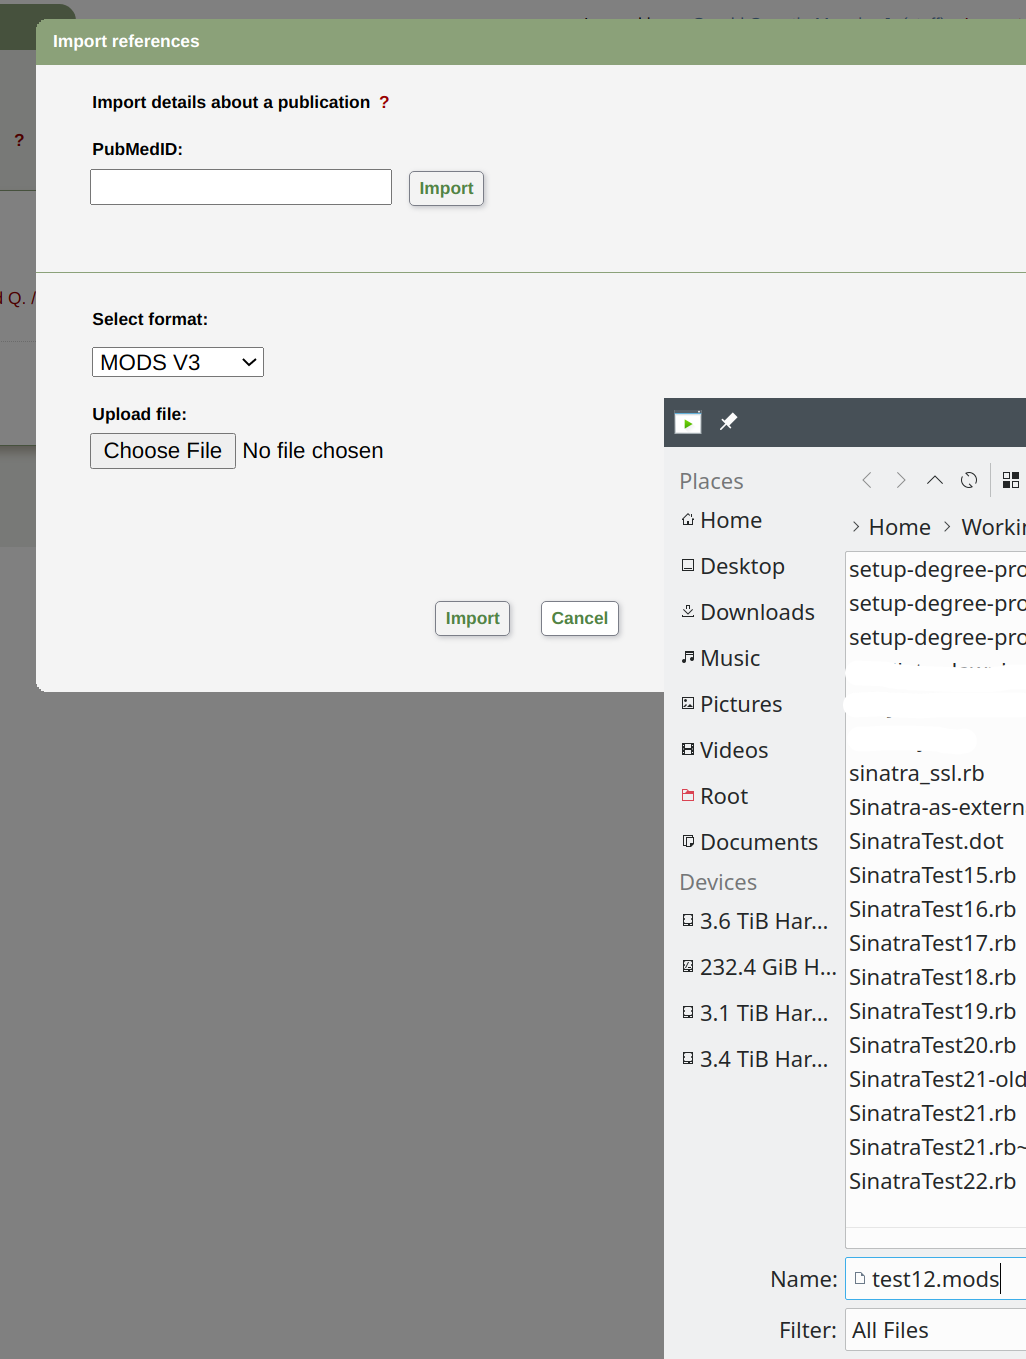
\includegraphics[width=1\textwidth]{README_notes/README-examiner-figures/import-2-Screenshot_20210626_234414.png}}
  \end{center}
  \caption[The import process – step 2]{The import process – step 2 – choose the MODV3 format and select a file to import}
  \label{fig:divaImport2}
\end{figure}
\FloatBarrier

\begin{figure}[!ht]
  \begin{center}
    \fbox{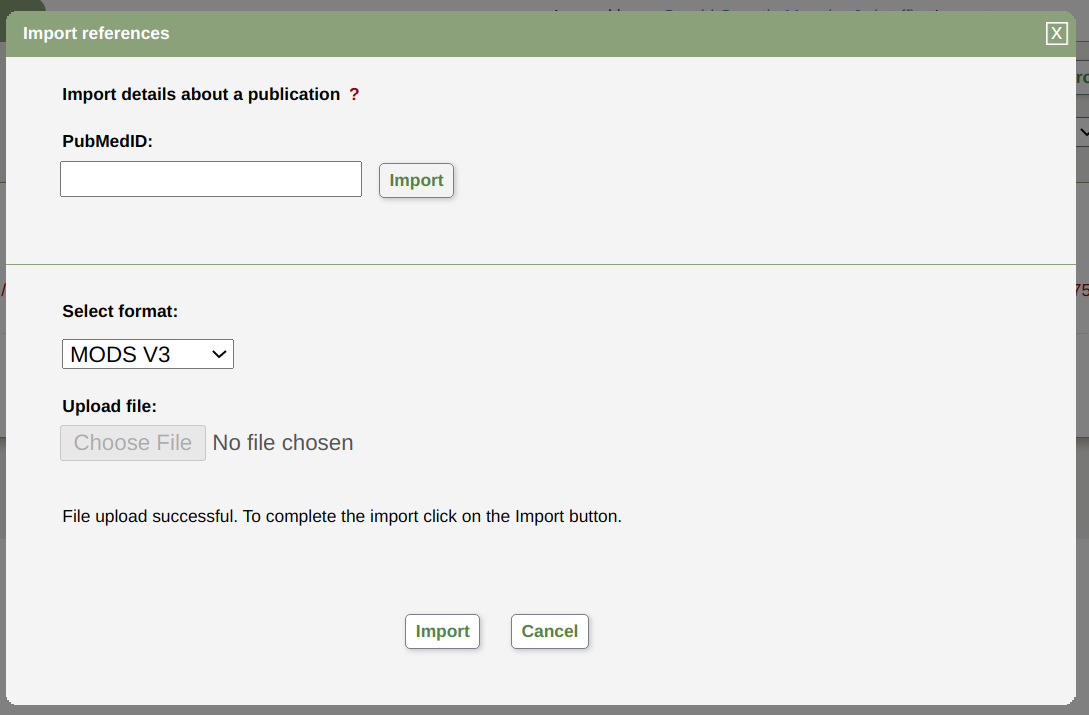
\includegraphics[width=1\textwidth]{README_notes/README-examiner-figures/import-3-Screenshot_20210626_234447.png}}
  \end{center}
  \caption[The import process – step 3]{The import process – step 3 – after clicking “Import” – it says that the file was successfully uploaded
Click on “Import” again to load the file. The MODS files is loaded and shown in \Cref{fig:divaImport4}.}
  \label{fig:divaImport3}
\end{figure}
\FloatBarrier

\begin{figure}[!ht]
  \begin{center}
    \fbox{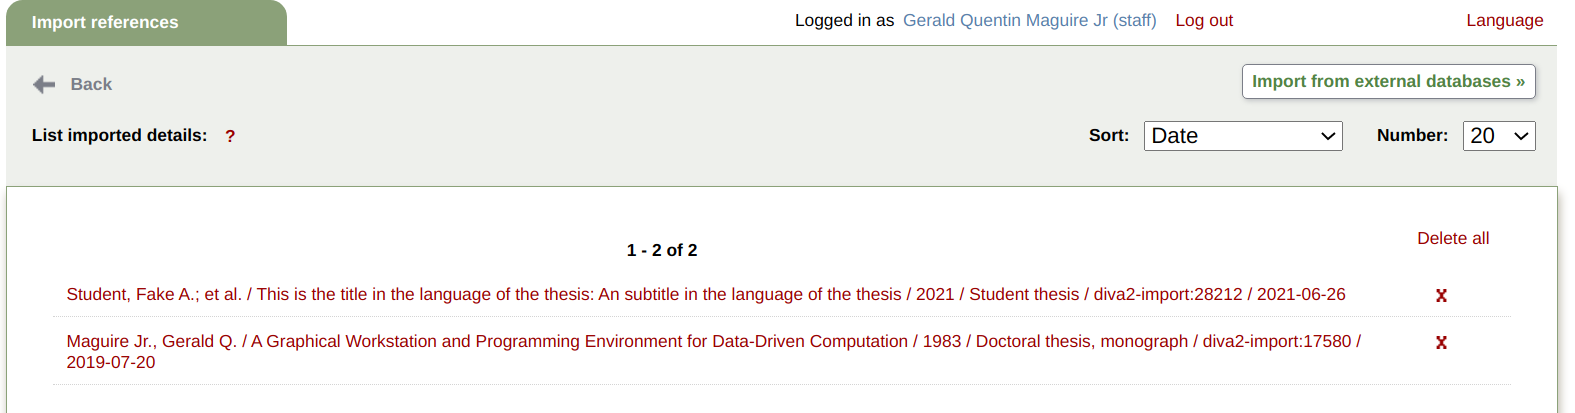
\includegraphics[width=1\textwidth]{README_notes/README-examiner-figures/import-4-Screenshot_20210626_234519.png}}
  \end{center}
  \caption[The import process – step 4]{The import process – step 4 – after clicking “Import” once more – you can see the file has been added to the list of imported files The imported document is shown in \Cref{fig:divaImport5} to \Cref{fig:divaImport12}.}
  \label{fig:divaImport4}
\end{figure}
\FloatBarrier

\begin{figure}[!ht]
  \begin{center}
    \fbox{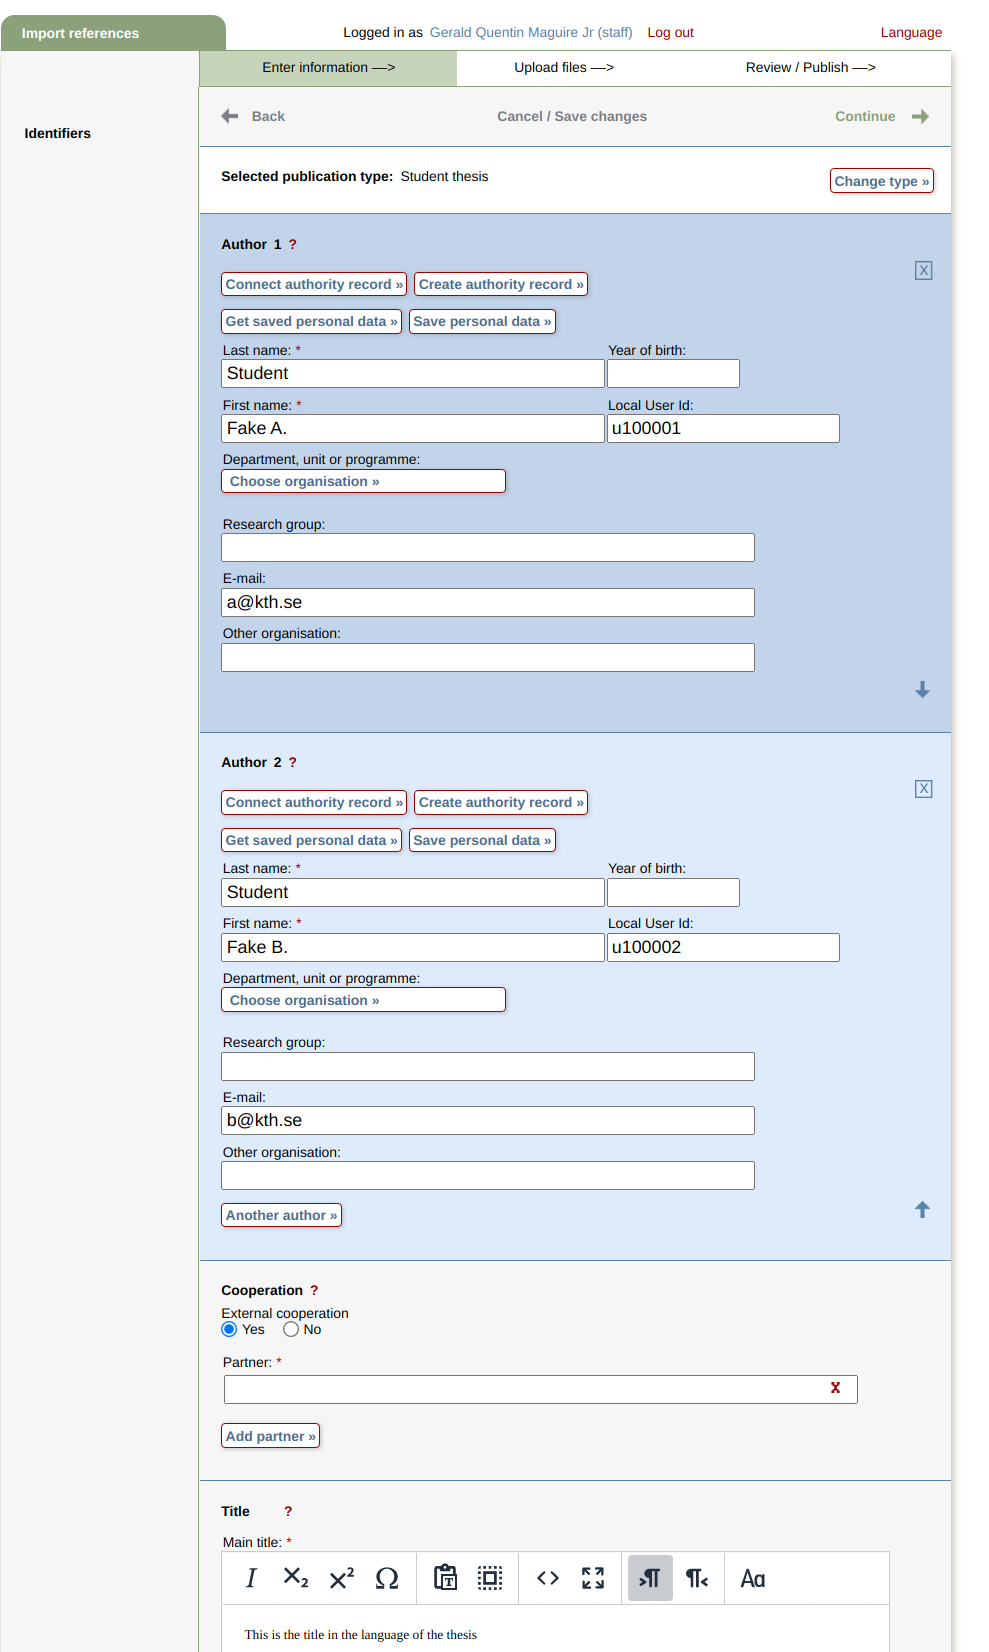
\includegraphics[width=0.8\textwidth]{README_notes/README-examiner-figures/import-a-Screenshot_20210626_234606.png}}
  \end{center}
  \caption[Imported document (part 1)]{Imported document (part 1)}
  \label{fig:divaImport5}
\end{figure}
\FloatBarrier

\begin{figure}[!ht]
  \begin{center}
    \fbox{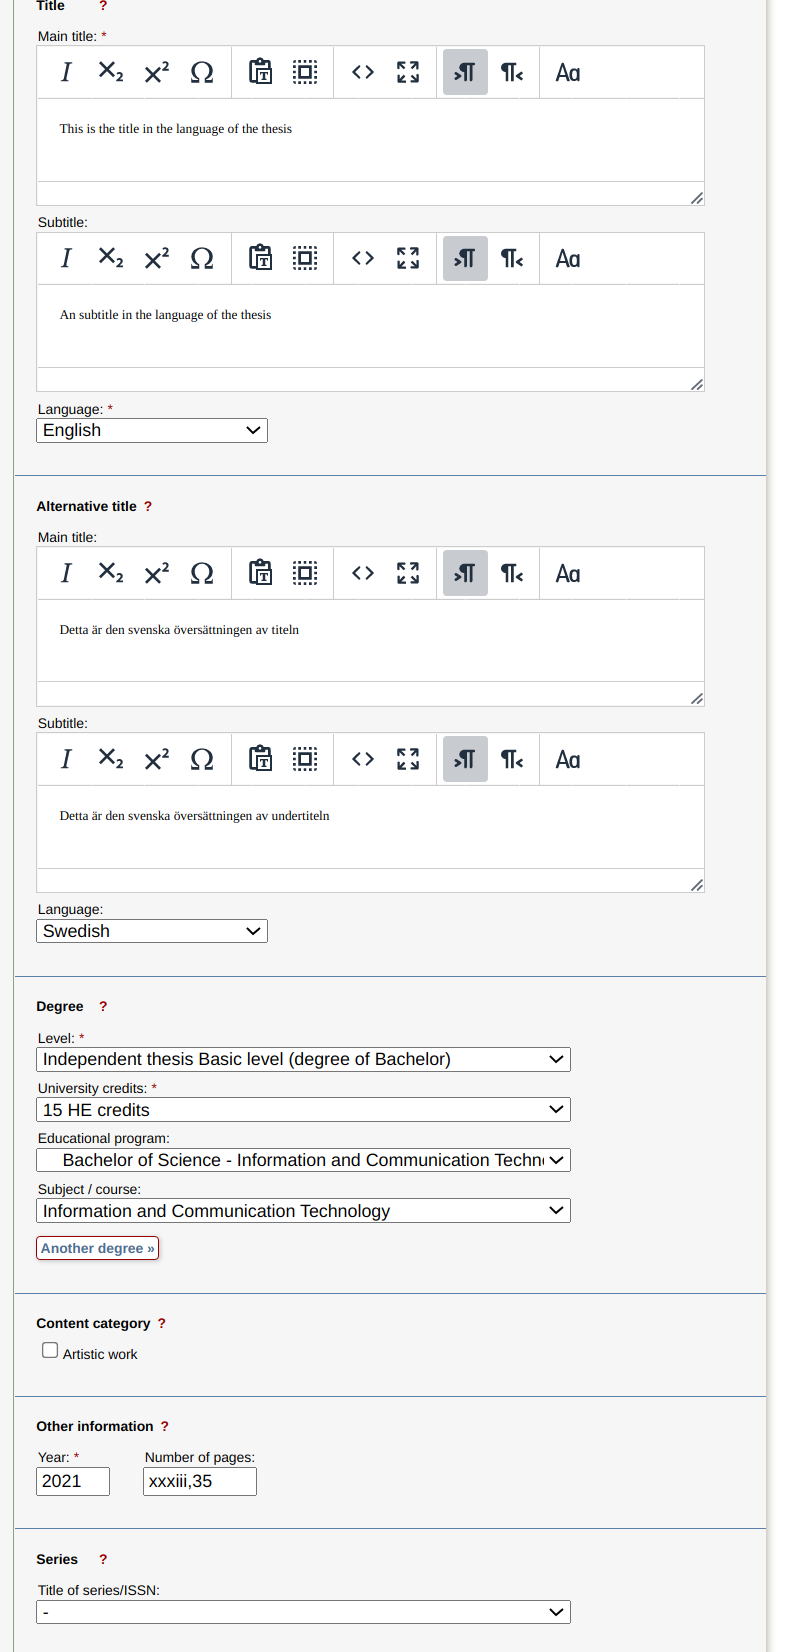
\includegraphics[width=0.65\textwidth]{README_notes/README-examiner-figures/import-b-Screenshot_20210626_234640.png}}
  \end{center}
  \caption[Imported document (part 2)]{Imported document (part 2) – Note that both the English and Swedish titles are shown as well as the information about which level, the number of university credits, the education al program, and the subject.- Additionally, the year and number of pages are shown.}
  \label{fig:divaImport6}
\end{figure}
\FloatBarrier

\begin{figure}[!ht]
  \begin{center}
    \fbox{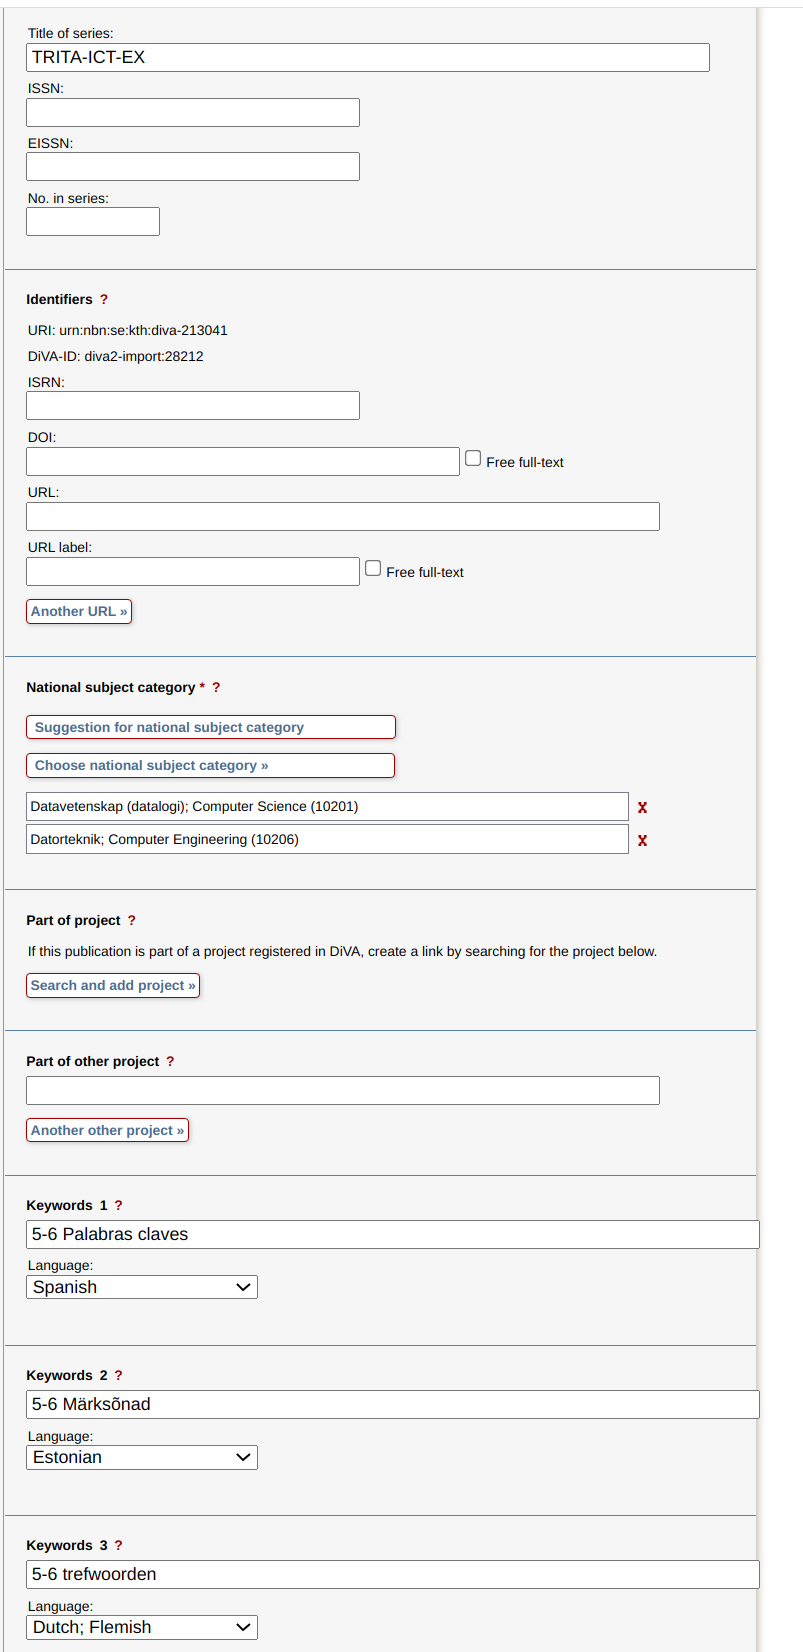
\includegraphics[width=0.65\textwidth]{README_notes/README-examiner-figures/import-c-Screenshot_20210626_234710.png}}
  \end{center}
  \caption[Imported document (part 3)]{Imported document (part 3) – Note that the number in the series is not being shown. The nation subject catergies specified in the JSON file are shown. Additionally, a number of the keyoards in different languages are shown.}
  \label{fig:divaImport7}
\end{figure}
\FloatBarrier

\begin{figure}[!ht]
  \begin{center}
    \fbox{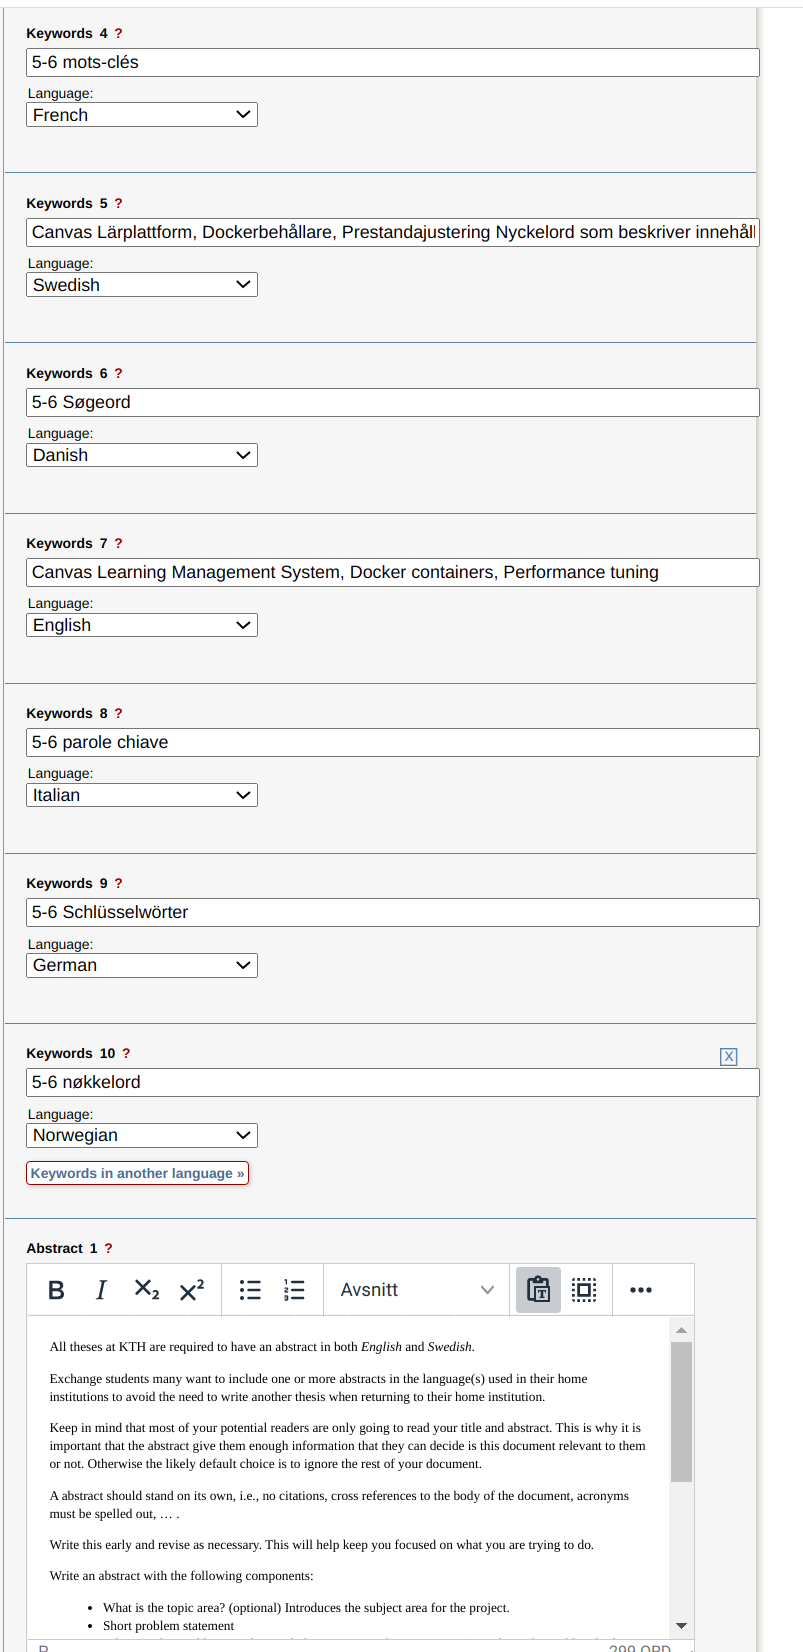
\includegraphics[width=0.65\textwidth]{README_notes/README-examiner-figures/import-d-Screenshot_20210626_234735.png}}
  \end{center}
  \caption[Imported document (part 4)]{Imported document (part 4) – more keywords are shown as well as the abstract in English}
  \label{fig:divaImport8}
\end{figure}
\FloatBarrier

\begin{figure}[!ht]
  \begin{center}
    \fbox{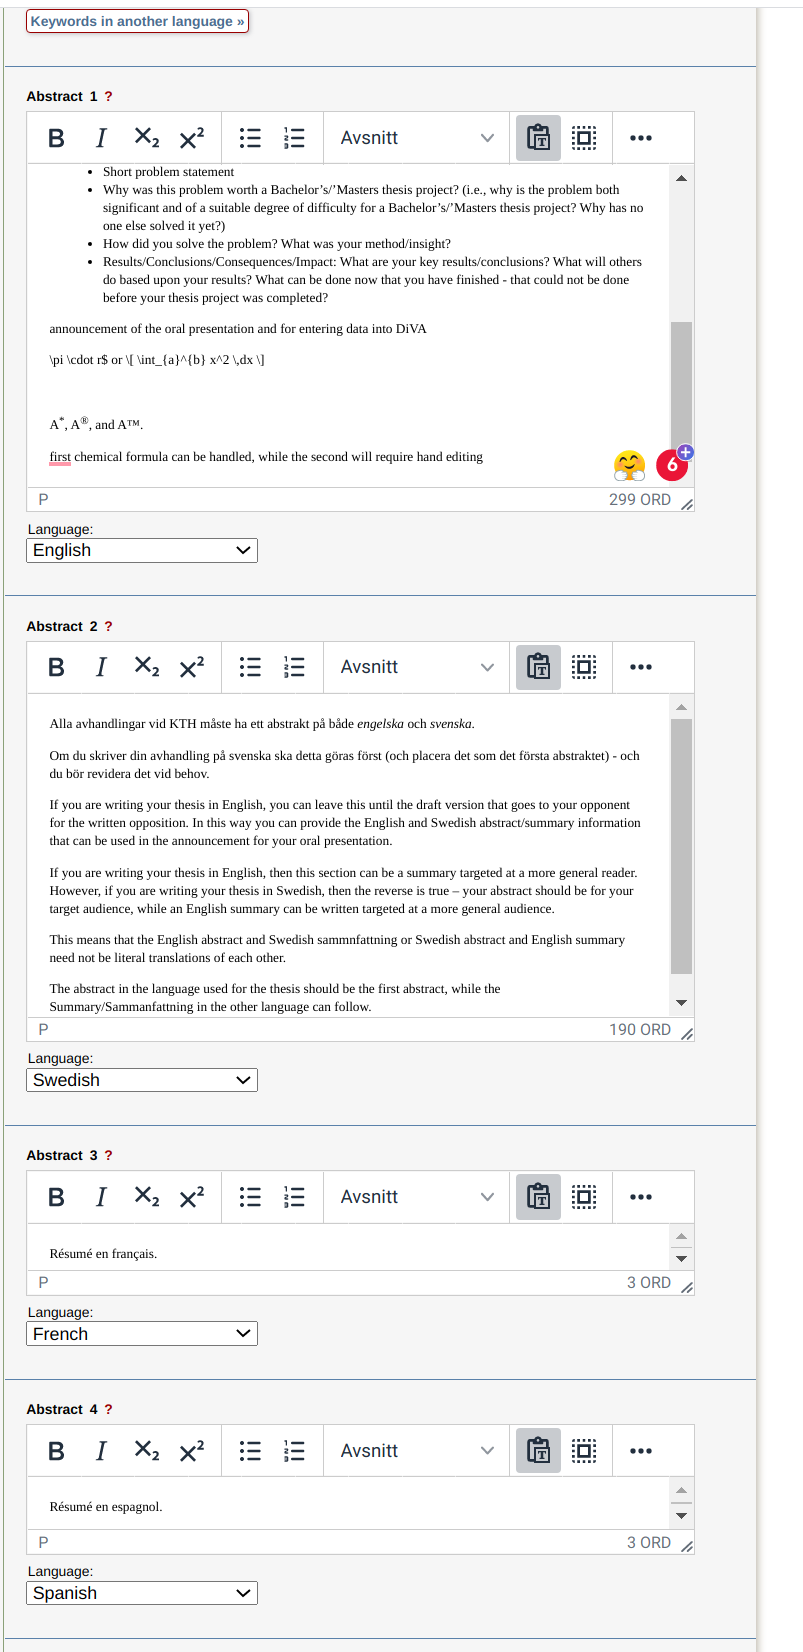
\includegraphics[width=0.65\textwidth]{README_notes/README-examiner-figures/import-e-Screenshot_20210626_235408.png}}
  \end{center}
  \caption{[Imported document (part 5)]Imported document (part 5) – the bottom of the Engish abstract is shown .- showing some of the formatted information that can be shown. Additionally, the Swedish and other abstracts are shown.}
  \label{fig:divaImport9}
\end{figure}
\FloatBarrier

\begin{figure}[!ht]
  \begin{center}
    \fbox{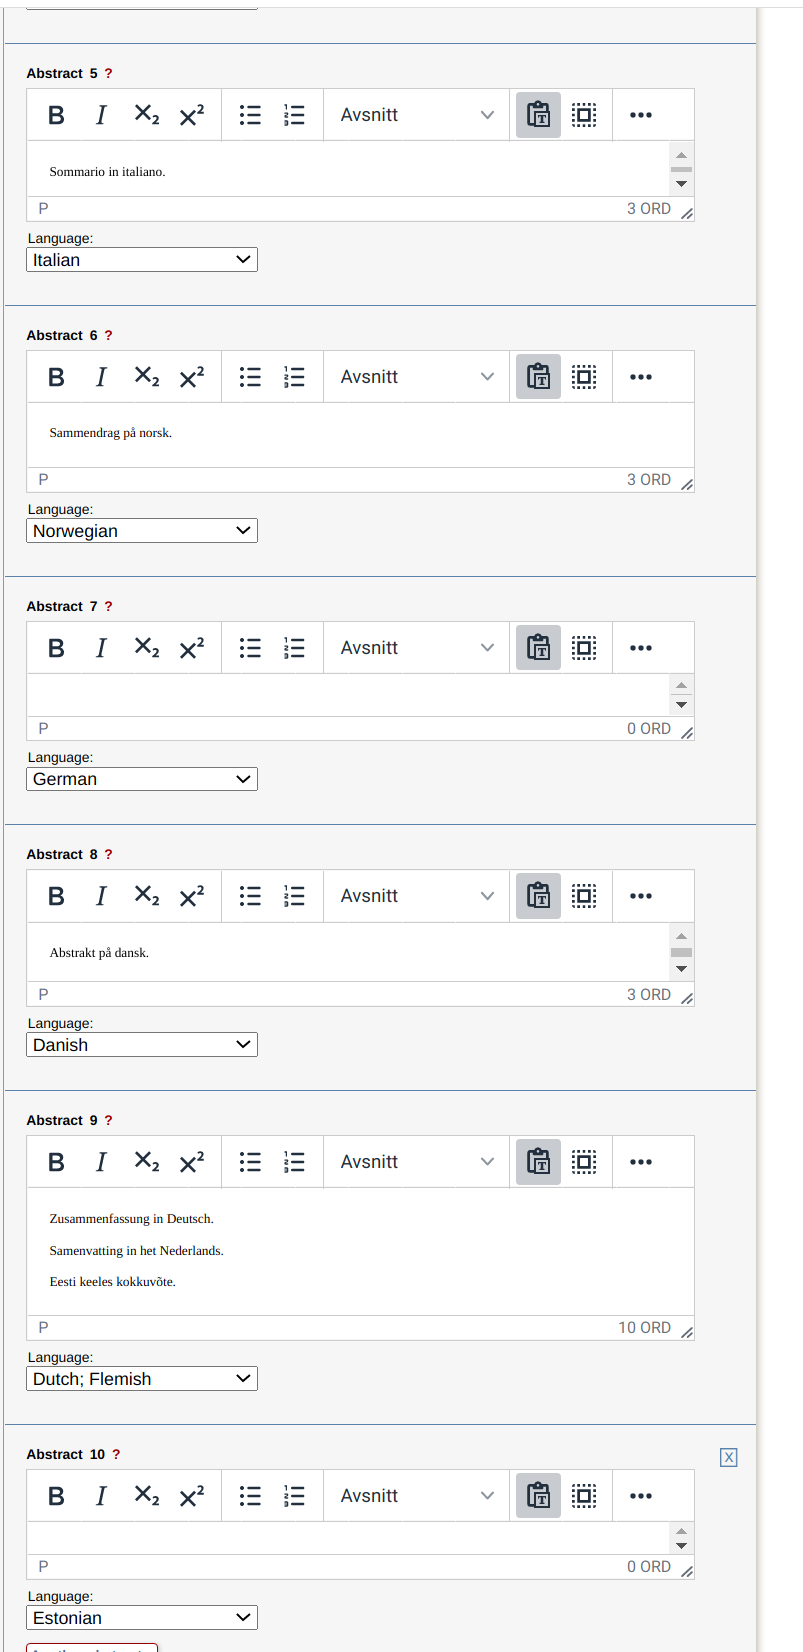
\includegraphics[width=0.7\textwidth]{README_notes/README-examiner-figures/import-f-Screenshot_20210626_235447.png}}
  \end{center}
  \caption[Imported document (part 6)]{Imported document (part 6) – yet more abstracts}
  \label{fig:divaImport10}
\end{figure}
\FloatBarrier
\Cref{fig:divaImport11} shows the three supervisors. The first two have KTH affiliations and the third is from an external organization.
\begin{figure}[!ht]
  \begin{center}
    \fbox{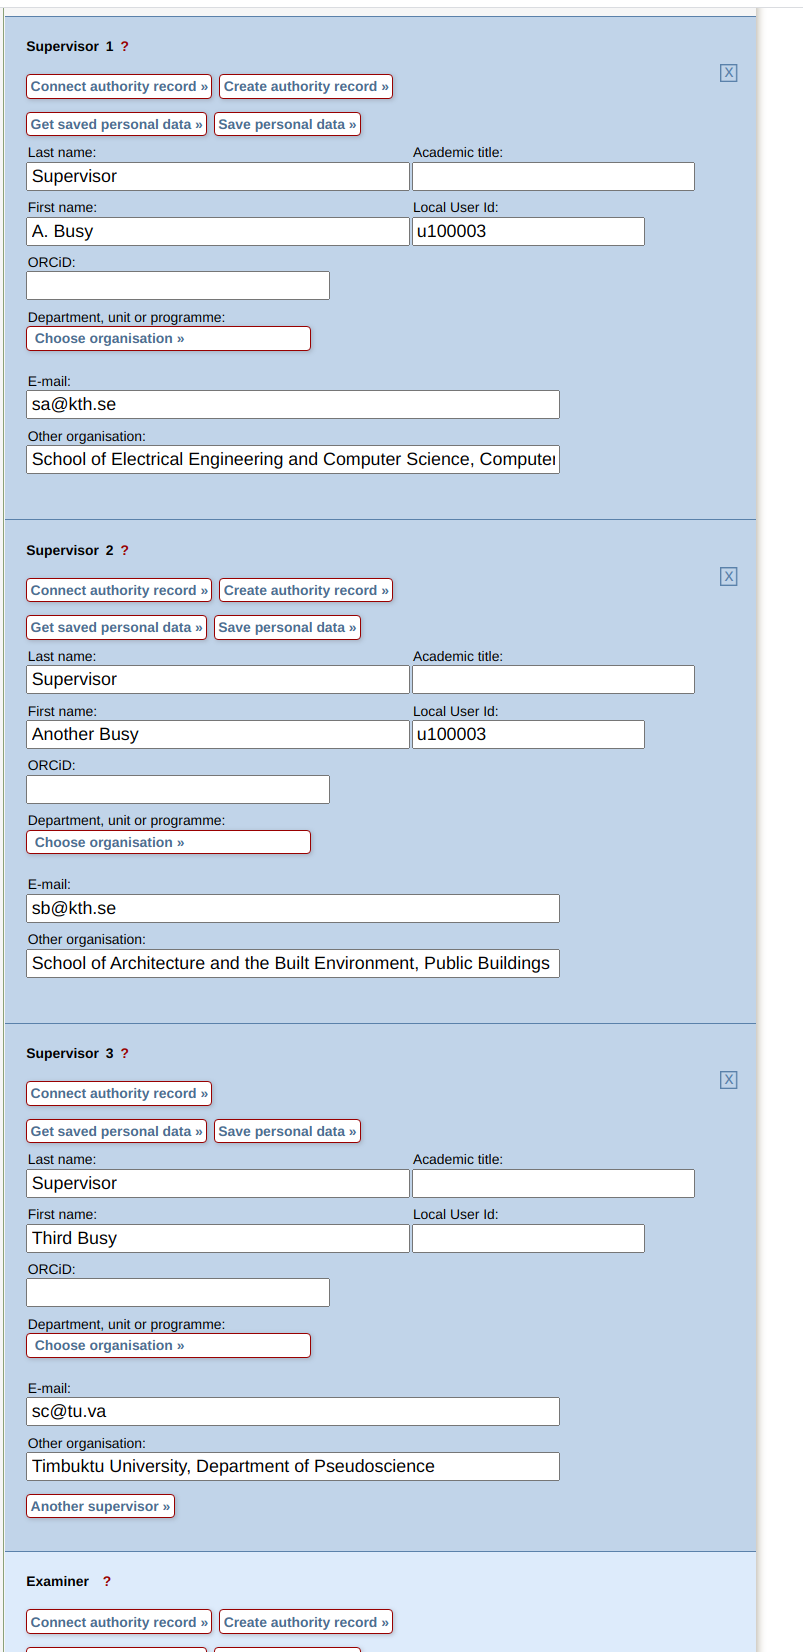
\includegraphics[width=0.7\textwidth]{README_notes/README-examiner-figures/import-g-Screenshot_20210626_235510.png}}
  \end{center}
  \caption[Imported document (part 7)]{Imported document (part 7) – the supervisors are shown}
  \label{fig:divaImport11}
\end{figure}
\newpage

\begin{figure}[!ht]
  \begin{center}
    \fbox{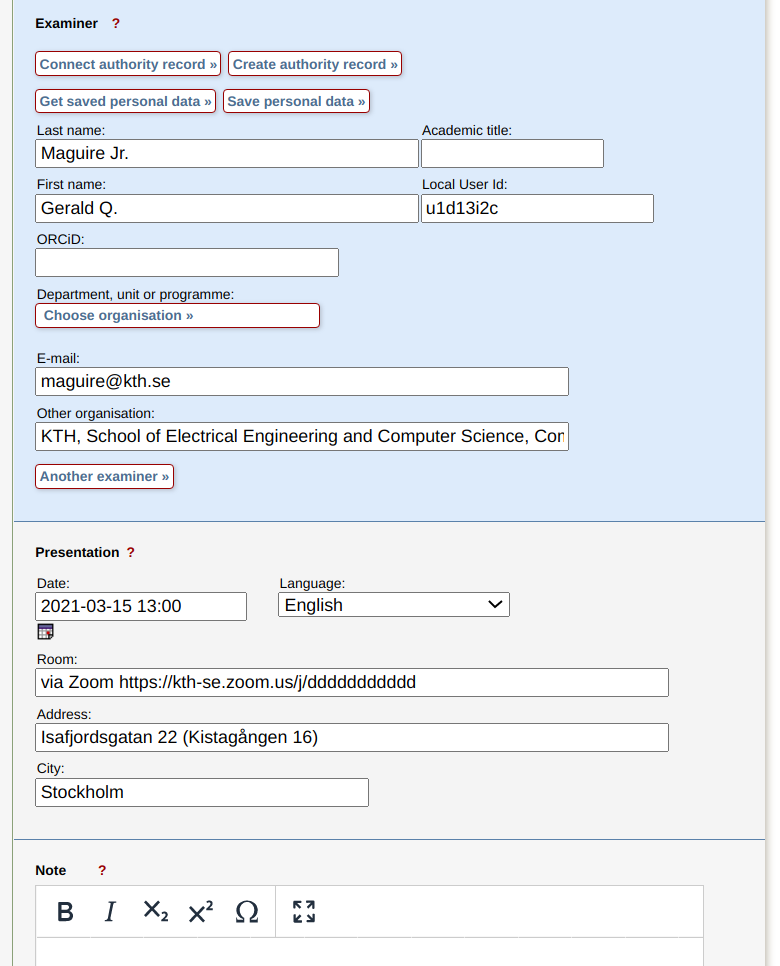
\includegraphics[width=1\textwidth]{README_notes/README-examiner-figures/import-h-Screenshot_20210626_235557.png}}
  \end{center}
  \caption[Imported document (part 8)]{Imported document (part 8) – the examiner is shown along with the information about the oral presentation}
  \label{fig:divaImport12}
\end{figure}
\clearpage


	

\subsection{Limitations}
I was initially unable to get the KTH affiliations correctly entered. I think that it is because I did not understand the description of how to do this at: \url{ https://wiki.epc.ub.uu.se/pages/viewpage.action?pageId=27466001}  where it says:
\babelpolyLangStart{swedish}
För att göra en sådan koppling skall dels ”affiliation” finnas i personelementet dels ett name-element med ID i xlink:href samt ett namePart-element med samma namn som affiliation. Om man har bägge nedanstående element i exemplet kommer Urban Ericsson automatiskt att kopplas till Universitetsbiblioteket i Uppsala vid importen. Om enbart personelementet finns men inte det andra kommer Urban Ericsson att få Uppsala universitet, Universitetsbiblioteket som ”Annat lärosäte” vid importen.
\babelpolyLangStop{swedish}
I did not find any examples of how to do what they describe. The result is that all of my affiliations information ended up in the "Other university" field.

I was also unable to get the issue number to appear, even though it seems to be set - since if you click on the box after the MODS import, it knows the value.  Note that for testing, I forced the TRITA series to be "TRITA-ICT-EX" since this is the actual series that is in the earlier (test) version of DiVA.

Finally, it seems that DiVA does not import the cooperation data at all: according to \url{https://wiki.epc.ub.uu.se/display/divainfo/Externt+samarbete}

The first two limitations have been overcome as described in\linebreak[4] \Cref{sec:limitationsOvercome}.

\subsection{Limitations overcome}
\label{sec:limitationsOvercome}
This section describes how two of the limitations were overcome.

\subsubsection{Entering number in series}
The first limitation to be over come was entering the particular number in the series for a TRITA number. \Cref{fig:numberInSeriesCorrectlyEntered} shows the value being entered. The error was in the structure of the object, the working version is shown in \Cref{lst:seriesNumber}. My earlier error was due to having the \texttt{<identifier type="issue number">2021:00</identifier>} \textit{within} the \texttt{<titleInfo>}.
 
 
\begin{figure}[!ht]
  \begin{center}
    \fbox{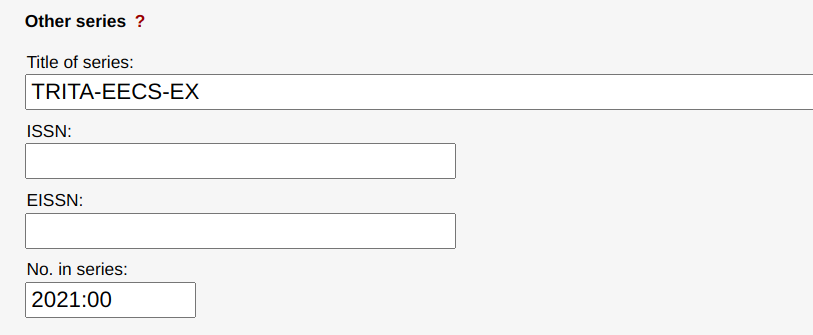
\includegraphics[width=1\textwidth]{README_notes/README-examiner-figures/Number_in_series_correctly_entered.png}}
  \end{center}
  \caption{Number in series correctly entered}
  \label{fig:numberInSeriesCorrectlyEntered}
\end{figure}
\Needspace*{8\baselineskip}
\begin{lstlisting}[language={XML}, caption={MODS data for series}, label=lst:seriesNumber]
<relatedItem  type="series">
	      <titleInfo><title>TRITA-EECS-EX</title>
		<identifier type="local">16855</identifier>
	      </titleInfo>
	      <identifier type="issue number">2021:00</identifier>
</relatedItem >
\end{lstlisting}

\FloatBarrier

\subsubsection{Including KTH affiliations}
Earlier those with KTH affiliations were appearing in the “Other organization” field. The error in my understanding was how the controlled fields for the KTH authors was being used\footnote{These so-called "controlled" fields have specific values that are permitted and these have numeric IDs assigned by the DiVA Consortium.}. We will start by looking at the two KTH affiliated supervisors (see \Cref{fig:twoKTHsupervisors}), the third supervisor (see \Cref{fig:thirdSupervisor}), and the examiner (see \Cref{fig:examiner}). The MODS data for these four people is shown in \Cref{lst:reducedModesExaminerAndSupervisors} and the “magic” \textbf{corporate name} MODS data is shown in \Cref{lst:reducedModesCorpNames}. The trick is that there needs to be corporate name MODS data for each of the possible affiliations – as this is the way that one passes the DiVA numeric code via the \texttt{xlink} information. Note that in the case of the examiner, two different affiliations were specified and there was a corporate name entry for each of them. Moreover, the key is just to have test extra corporate name entries, only one needs to be for the publishers, as shown in \Cref{lst:reducedModesCorpNames} – with the results in \Cref{fig:twoSupervisorsReducedMODS} and shown \Cref{fig:examinerReducedMODS}.

\textbf{NB}: The ICT affiliations (and DiVA codes) were used and the pictures are all from the test DiVA environment: \url{https://kth.test.diva-portal.org/dream/import/importList.jsf}.

\begin{figure}[!ht]
  \begin{center}
    \fbox{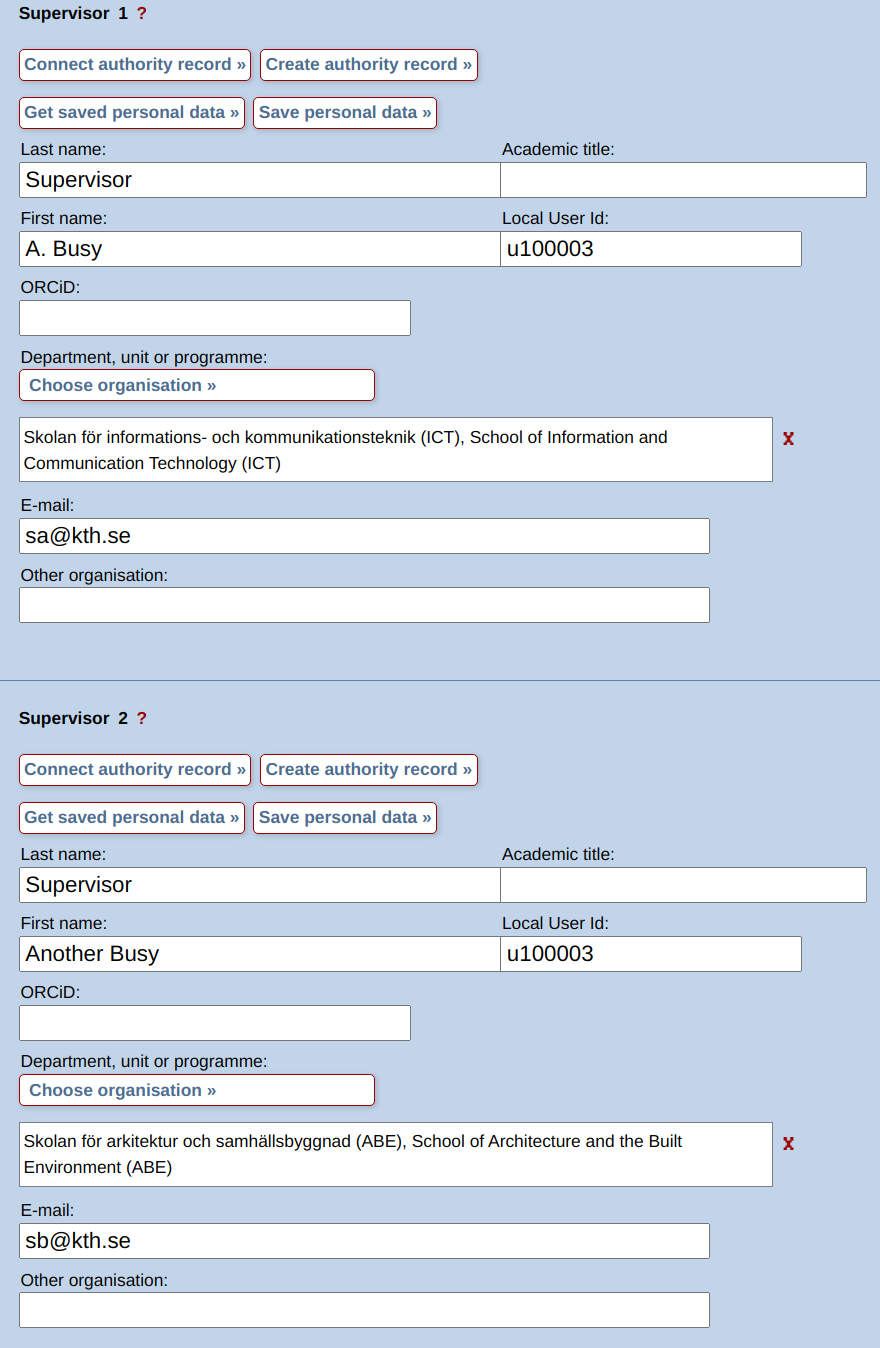
\includegraphics[width=0.9\textwidth]{README_notes/README-examiner-figures/two_KTH_supervisors_in_different_schools.png}}
  \end{center}
  \caption{Two KTH supervisors in different schools}
  \label{fig:twoKTHsupervisors}
\end{figure}
\FloatBarrier
\begin{figure}[!ht]
  \begin{center}
    \fbox{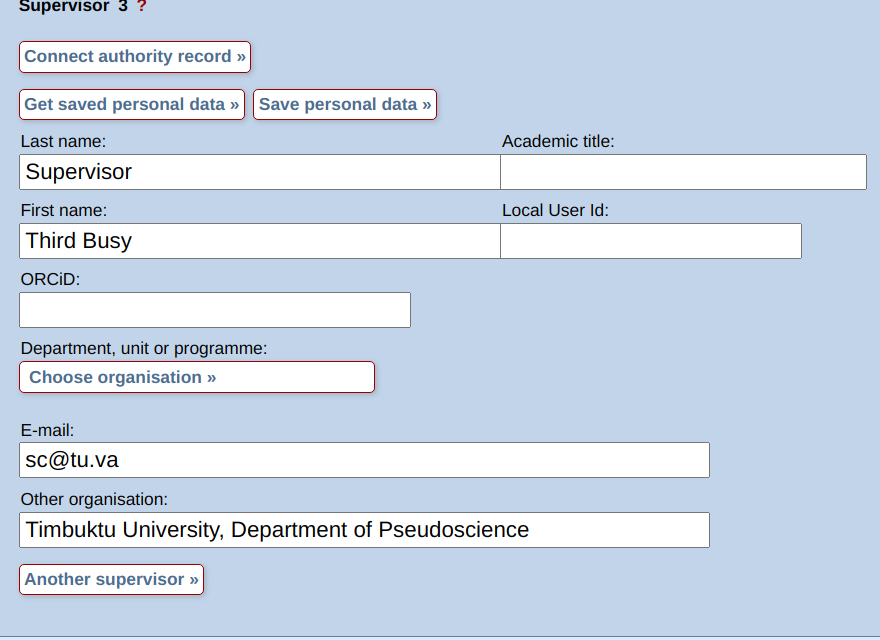
\includegraphics[width=1\textwidth]{README_notes/README-examiner-figures/third_supervisor.png}}
  \end{center}
  \caption{Third supervisor}
  \label{fig:thirdSupervisor}
\end{figure}
\FloatBarrier
\begin{figure}[!ht]
  \begin{center}
    \fbox{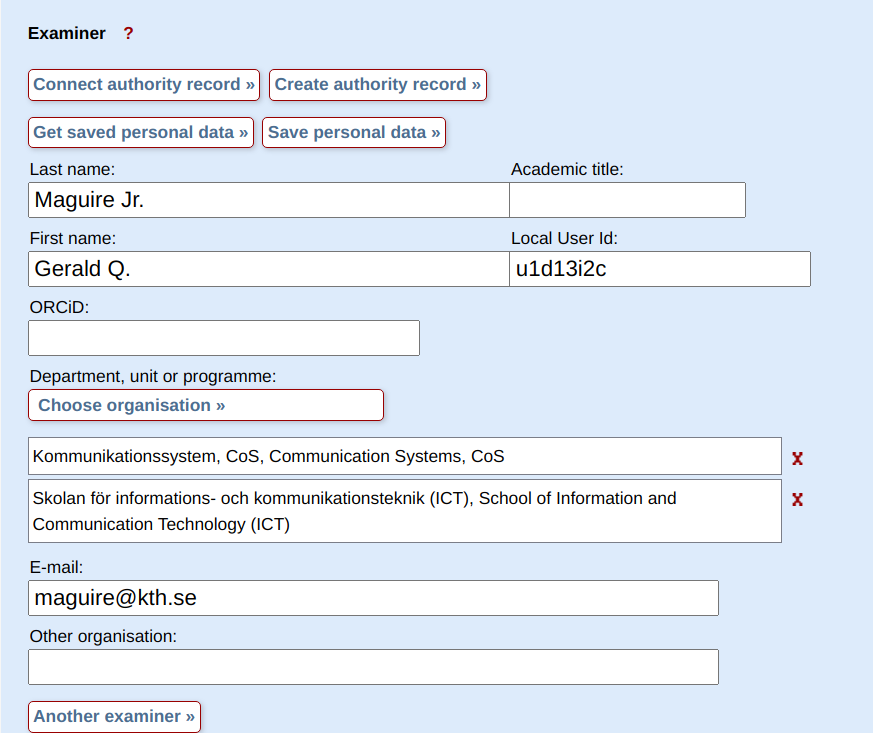
\includegraphics[width=1\textwidth]{README_notes/README-examiner-figures/examiner_affiliation.png}}
  \end{center}
  \caption{Examiner}
  \label{fig:examiner}
\end{figure}
\clearpage

\begin{lstlisting}[language={XML}, caption={MODS data for the supervisors and examiners}, label=lst:reducedModesExaminerAndSupervisors]
<name type="personal" authority="kth" xlink:href="u1d13i2c">
      <namePart type="family">Maguire Jr.</namePart>
      <namePart type="given">Gerald Q.</namePart>
      <description>email=maguire@kth.se</description>
      <affiliation>KTH, Skolan för informations- och kommunikationsteknik (ICT), Kommunikationssystem, CoS</affiliation>
      <affiliation>KTH, Skolan för informations- och kommunikationsteknik (ICT)</affiliation>
      <role><roleTerm type="code" authority="marcrelator">mon</roleTerm></role>
</name>

<name type="personal" authority="kth" xlink:href="u100003">
      <namePart type="family">Supervisor</namePart>
      <namePart type="given">A. Busy</namePart>
      <affiliation>KTH, Skolan för informations- och kommunikationsteknik (ICT)</affiliation>
      <description>email=sa@kth.se</description>
      <role><roleTerm type="code" authority="marcrelator">ths</roleTerm></role>
</name>

<name type="personal" authority="kth" xlink:href="u100003">
      <namePart type="family">Supervisor</namePart>
      <namePart type="given">Another Busy</namePart>
      <affiliation>KTH, Skolan för arkitektur och samhällsbyggnad (ABE)</affiliation>
      <description>email=sb@kth.se</description>
      <role><roleTerm type="code" authority="marcrelator">ths</roleTerm></role>
</name>

<name type="personal">
      <namePart type="family">Supervisor</namePart>
      <namePart type="given">Third Busy</namePart>
      <affiliation>Timbuktu University, Department of Pseudoscience</affiliation>
      <description>email=sc@tu.va</description>
      <role><roleTerm type="code" authority="marcrelator">ths</roleTerm></role>
</name>
\end{lstlisting}
\clearpage

\begin{lstlisting}[language={XML}, caption={Corporate name data in MODS data for the affiliations}, label=lst:reducedModesCorpNames]
<name type="corporate" authority="kth" xlink:href="5994">
      <namePart>KTH</namePart>
      <namePart>Skolan för informations- och kommunikationsteknik (ICT)</namePart>
      <role><roleTerm type="code" authority="marcrelator">pbl</roleTerm></role>
</name>

<name type="corporate" authority="kth" xlink:href="5998">
      <namePart>KTH</namePart>
      <namePart>Skolan för informations- och kommunikationsteknik (ICT)</namePart>
      <namePart>Kommunikationssystem, CoS</namePart>
      <role><roleTerm type="code" authority="marcrelator">pbl</roleTerm></role>
</name>

<name type="corporate" authority="kth" xlink:href="5850">
      <namePart>KTH</namePart>
      <namePart>Skolan för arkitektur och samhällsbyggnad (ABE)</namePart>
      <role><roleTerm type="code" authority="marcrelator">pbl</roleTerm></role>
</name>
\end{lstlisting}

\begin{lstlisting}[language={XML}, caption={Reduced MODS for corporate names more}, label=lst:reducedModesCorpNamesMore]
<name type="corporate" authority="kth" xlink:href="5994">
      <namePart>KTH</namePart>
      <namePart>Skolan för informations- och kommunikationsteknik (ICT)</namePart>
      <role><roleTerm type="code" authority="marcrelator">pbl</roleTerm></role>
</name>
<name type="corporate" authority="kth" xlink:href="5998">
      <namePart>KTH</namePart>
      <namePart>Skolan för informations- och kommunikationsteknik (ICT)</namePart>
      <namePart>Kommunikationssystem, CoS</namePart>
</name>
<name type="corporate" authority="kth" xlink:href="5850">
      <namePart>KTH</namePart>
      <namePart>Skolan för arkitektur och samhällsbyggnad (ABE)</namePart>
</name>
\end{lstlisting}
\clearpage

\begin{figure}[!ht]
  \begin{center}
    \fbox{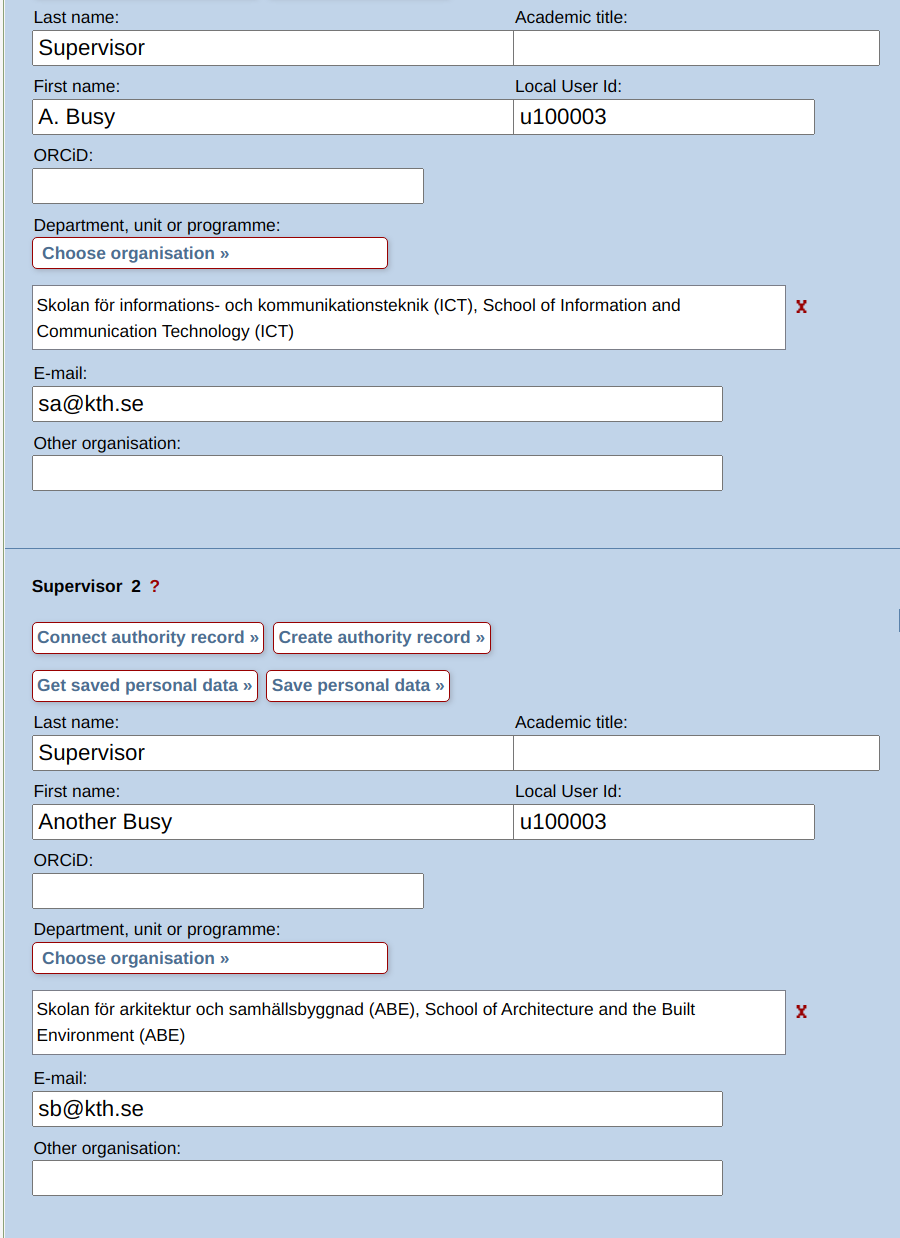
\includegraphics[width=1\textwidth]{README_notes/README-examiner-figures/two_supervisors_reduced_mods.png}}
  \end{center}
  \caption{The two supervisors with the reduced MODS for corporate names}
  \label{fig:twoSupervisorsReducedMODS}
\end{figure}

\begin{figure}[!ht]
  \begin{center}
    \fbox{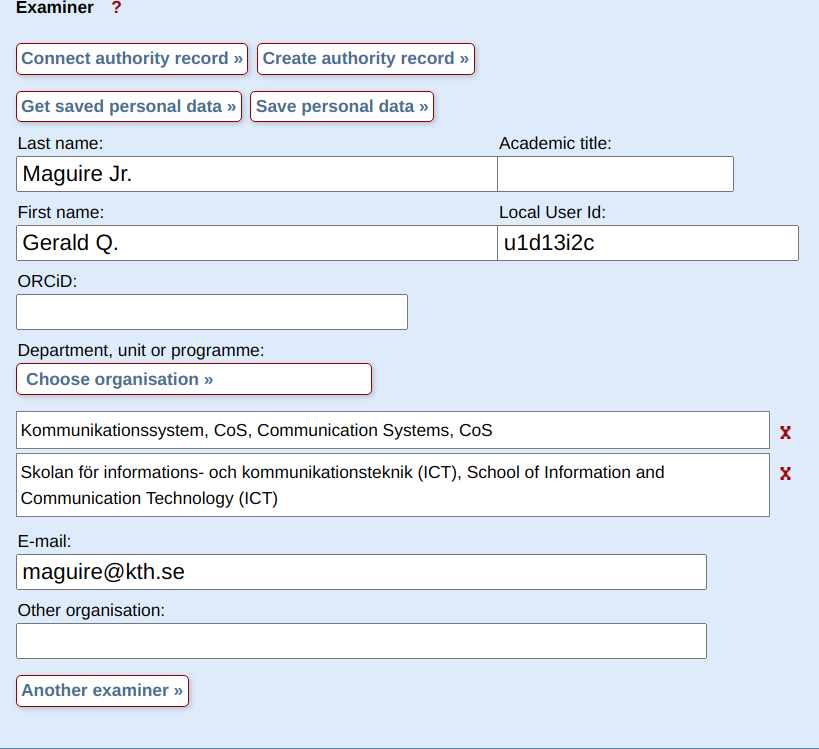
\includegraphics[width=1\textwidth]{README_notes/README-examiner-figures/examiner_with_reduced_mods.png}}
  \end{center}
  \caption{The examiner with the reduced MODS for corporate names}
  \label{fig:examinerReducedMODS}
\end{figure}
\clearpage

\section{Some enhancements}
\label{sec:someEhnahncements}
The enhancements described in \Cref{sec:enhancementsToTemplate} are enhancements to the template and supporting programs to avoid the user having to enter some information on the command line when making a cover and to make the information better available for a future DiVA entry. The enhancements described in \Cref{sec:betterSupportForMathInAbstracts} are to better support mathematical expressions in abstracts. \Cref{sec:AcronymsInAbstracts} describes support for acronyms in abstracts. \Cref{sec:URLSinAbstracts} describes the state of support for URLs in abstracts. \Cref{sec:gettingPDFfromCanvasAssignment} describes a program that can extract an assignment from a Canvas course room and optionally feed it to the program to extract the pseudo-JSON information.

\subsection{Enhancements to template and supporting programs}
\label{sec:enhancementsToTemplate}
Add better support for the subject area (or areas in the case of a student doing both a Civ. Ing. Degree and a Master’s degree).

\subsection{Better support for mathematical expressions in abstracts}
\label{sec:betterSupportForMathInAbstracts}
\LaTeX~in the abstracts is passed through to the pseudo JSON in the “For DIVA” text at the end of the thesis. When preparing this text for Cortina calendar entries or for the announcement in the Canvas course room (and for the calendar event in the course room) some simple \LaTeX~commands are converted to HTML. As few abstracts (in the many abstracts that I looked at in DiVA) have equations I have only done these few transformations. However, if there were to be more use of equations, then there is probably a need to support them for the different platforms (Cortina (see Appendix~\ref{sec:BetterSupportforMathinCortina}), DiVA (see Appendix~\ref{sec:SupportForMathematicsInDiVA}), and Canvas (see Appendix~\ref{sec:betterSupportMathInCortinaAndCourseCalendar})).


\subsubsection{Better support for mathematics in Canvas course announcement and course calendar}
\label{sec:betterSupportMathInCortinaAndCourseCalendar}
As of 2021-06-18, MathJAX and URLs are now supported in the Canvas course room announcement and calendar.
Using the Overleaf project: \url{https://www.overleaf.com/read/qsyddnhhvkgr} to provide a test source document. The results can be seen in \Cref{fig:equationsInAnnouncement}. These results and the results shown in Appendix~\ref{sec:BetterSupportforMathinCortina} were generated using the commands in \Cref{lst:jsonToCalendar3}.
\begin{figure}[!ht]
  \begin{center}
    \fbox{
\includegraphics[width=1\textwidth]{README_notes/README-examiner-figures/announcement_with_equation.png}}
  \end{center}
  \caption{Examples of equations in an announcement}
  \label{fig:equationsInAnnouncement}
\end{figure}
\FloatBarrier
\Needspace*{8\baselineskip}
\begin{lstlisting}[language={bash}, caption={Commands to produce the JSON and make the calendar entries and announcement}, label=lst:jsonToCalendar3]
./extract_pseudo_JSON-from_PDF.py --pdf abstracts_with_equations_in_them.pdf --json eqtest.json
./JSON_to_calendar.py -c 11 --config config-test.json --json eqtest.json
\end{lstlisting}

\FloatBarrier

Note that block/display math are displayed in the Canvas summary for the announcements and cause Canvas to stop summarizing the abstract. The cause for this is not yet known, but has been reported to e-learning ([\#ID:KTH-INC-3677258\#]) and I have blogged about it in the Canvas Community. An example of the equation being displayed in the summary of the announcement is shown in \Cref{fig:announcementSummary}. The announcement is shown in \Cref{fig:announcementWithEquation} while \Cref{lst:HTMLannouncement} shows the HTML for this announcement.

\begin{figure}[!ht]
  \begin{center}
    \fbox{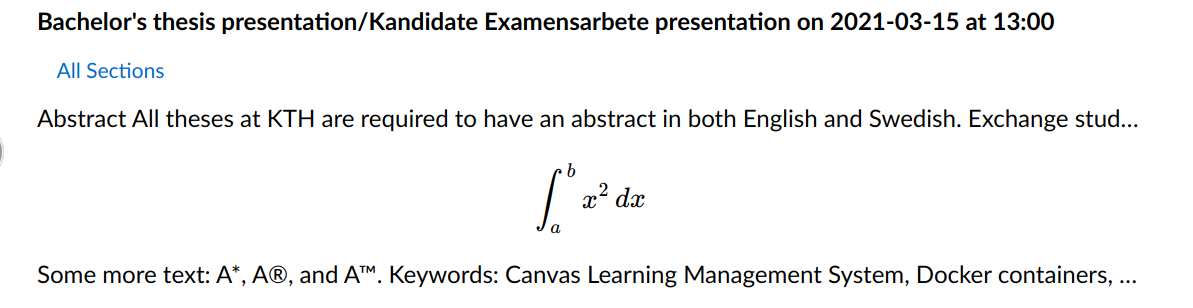
\includegraphics[width=1\textwidth]{README_notes/README-examiner-figures/Announcement_summary.png}}
  \end{center}
  \caption{Announcement summary}
  \label{fig:announcementSummary}
\end{figure}
\FloatBarrier

\begin{figure}[!ht]
  \begin{center}
    \fbox{
\includegraphics[width=1\textwidth]{README_notes/README-examiner-figures/announcement_with_equation.png}}
  \end{center}
  \caption{Announcement with equation}
  \label{fig:announcementWithEquation}
\end{figure}
\FloatBarrier
\Needspace*{18\baselineskip}
\begin{lstlisting}[language={HTML}, caption={HTML for the announcement}, label=lst:HTMLannouncement]
<h2 lang="en">Abstract</h2>
<p>All theses at KTH are required to have an abstract in both <i>English</i> and <i>Swedish</i>.</p>
<p>Exchange students many want to include one or more abstracts in the language(s) used in their home institutions to avoid the need to write another thesis when returning to their home institution.</p>
<p><span class="math-tex">\(\pi \cdot r\)</span> or <span class="math-tex">\[ \int_{a}^{b} x^2 \,dx \]</span></p>
<p>Some more text: A<sup>*</sup>, A<sup>&reg;</sup>, and A&trade;.</p>
<p><strong>Keywords:</strong> <em>Canvas Learning Management System, Docker containers, Performance tuning </em></p>
\end{lstlisting}


Via XXXXX at IT-support, I raised the question about why the block equations were appearing in the summary of the announcement.

The response from Instructure support regarding the block equations showing up in the summary of the announcements was\footnote{Note that the URLs have been added in parenthesis.}:
\begin{quote}
Thank you for reaching back out.  I did some testing on this and I have a few things to point out and some follow up questions.

First off, the syntax of the block equation isn't the officially supported format.  The inline equation is correct with the \textbackslash(...\textbackslash) delimiters, but the block equation should be formatted with dollar signs, as \$\$...\$\$.  I see the square bracket delimiters \textbackslash[...\textbackslash] are working currently, but this is not the officially supported format and may not always work.  Information on this can be found in these release notes (\url{https://community.canvaslms.com/t5/Canvas-Releases/Canvas-Release-Notes-2021-02-20/ta-p/434781\#toc-hId-698876024}).

Regardless of that though, I wanted to get clarification on the issue at hand.  When I open the announcement, I see both the inline and block equations, but I see only the block equation when viewing it on the main Announcements page.  Is this specifically what you're reporting?  (sandbox screenshot for reference (\url{https://share.getcloudapp.com/jkuPOKRD})  If so, this is because the Announcements page only shows a snippet of the text, so an inline equation beyond the point the text is truncated isn't treated any differently than the rest of the text not shown.  It is interesting that Canvas decides to show the block equation in this view though.  Having that removed from the preview would best be submitted as a feature request (\url{https://community.canvaslms.com/t5/forums/postpage/board-id/ideas/search-before-post-mode/true} ).

If the issues you're reporting are when the full announcement is open, I'm not seeing the same behavior on this end.  If that's the case, can you provide a screenshot of what you're seeing?  And does the behavior persist in a different browser?

Let me know if I've misinterpreted anything or if there are any other questions as well.  We'll be happy to help.  Thanks and have a great day!"
\end{quote}

The response from someone at Instructure shows that Instructure got the same behavior from the block equations in the snippets of the announcements.  A screenshot of this behavior is shown in \Cref{fig:screenSHotOfBlockEquation}. However, their solution for this is to suggest that we submit a feature request. 

\begin{figure}[!ht]
  \begin{center}
    \fbox{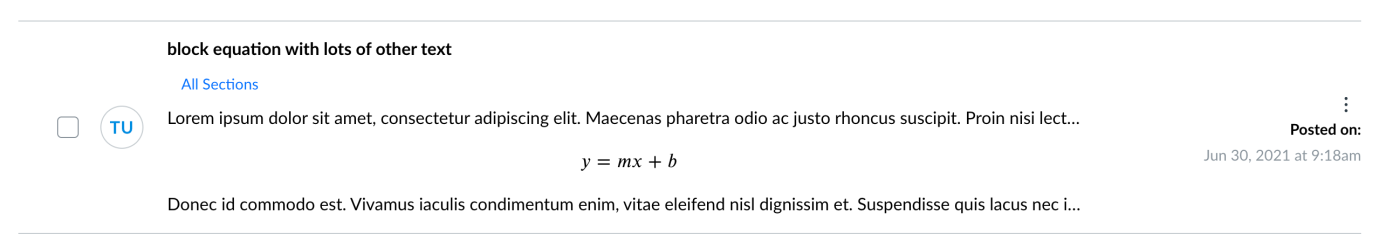
\includegraphics[width=1\textwidth]{README_notes/README-examiner-figures/block_equation_in_Canvas.png}}
  \end{center}
  \caption{The screenshot mentioned above}
  \label{fig:screenSHotOfBlockEquation}
\end{figure}
\FloatBarrier



\subsubsection{Better support for mathematics in Cortina}
\label{sec:BetterSupportforMathinCortina}

YYYYYY indicated that CORTINA supports mathematical expressions using a class name of “math-tex” and gave an example:
%% <span class=\"math-tex\">\\(x = {-b \\pm \\sqrt{b^2-4ac} \\over 2a}\\)</span>
\begin{quote}
$<$span class=\textbackslash"math-tex\textbackslash"$>$\textbackslash\textbackslash(x = {-b \textbackslash\textbackslash pm \textbackslash\textbackslash sqrt\{b\^{}2-4ac\} \textbackslash\textbackslash over 2a}\textbackslash\textbackslash)$<$/span$>$
\end{quote}


\noindent He also noted that Cortina does not allow images in paragraphs, so the solutions for Cortina and DiVA have to be different.

An important note about the above example is that \textbackslash over is deprecated and one should use \textbackslash frac{}{} or one of its variance instead; hence, I used this version of the equation in my source \LaTeX~file.
\clearpage
\Cref{fig:cortinaExample1} shows the entry in the Cortina calendar, while \Cref{fig:cortinaExample2} and \Cref{fig:cortinaExample3} show zoomed in views of the equations.
\begin{figure}[!ht]
  \begin{center}
    \fbox{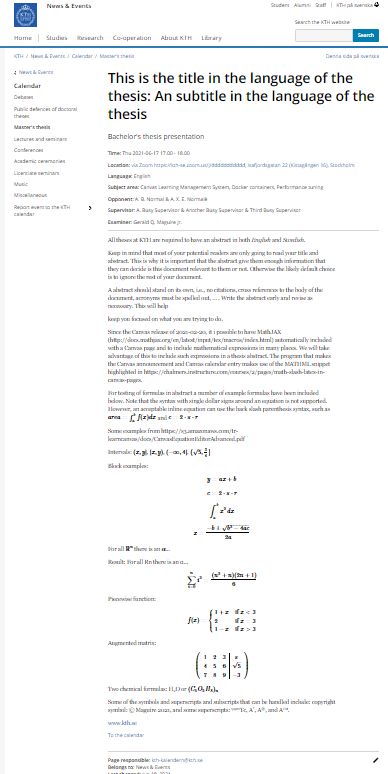
\includegraphics[width=0.65\textwidth]{README_notes/README-examiner-figures/Cortina_exaample1.png}}
  \end{center}
  \caption{Equations in Cortina calendar entry}
  \label{fig:cortinaExample1}
\end{figure}
\FloatBarrier

\begin{figure}[!ht]
  \begin{center}
    \fbox{\includegraphics[width=1\textwidth]{README_notes/README-examiner-figures/cortina-eqn-zoom1.png}}
  \end{center}
  \caption{Zoom in on part of the Cortina calendar entry}
  \label{fig:cortinaExample2}
\end{figure}
\FloatBarrier

\begin{figure}[!ht]
  \begin{center}
    \fbox{\includegraphics[width=1\textwidth]{README_notes/README-examiner-figures/cortina-eqn-zoom2.png}}
  \end{center}
  \caption{Zoom in on lower part of the Cortina calendar entry}
  \label{fig:cortinaExample3}
\end{figure}
\FloatBarrier
 

\subsubsection{Support for mathematics in DiVA}
\label{sec:SupportForMathematicsInDiVA}
In contrast to Canvas and Cortina, DiVA uses pictures (although these can have a \LaTeX~expression as an “alt” description of the image contents).
The code does not (yet) support the addition of equations to the DiVA entry of the abstracts.
The current DiVA user interface seems to strip out the math-tex classes, \ie 

% <span class='math-tex'>\[ \int_{a}^{b} x^2 \,dx \]</span> 
\begin{quote}
$<$span class=\textbackslash"math-tex\textbackslash"$>$\textbackslash [ \textbackslash int\_\{a\}\^{}\{b\} x\^{}  \textbackslash ,dx \textbackslash ] $<$/span$>$
\end{quote}

becomes simply:
% \[ \int_{a}^{b} x^2 \,dx \]
\begin{quote}
\textbackslash [ \textbackslash int\_\{a\}\^{}\{b\} x\^{}2  \textbackslash ,dx \textbackslash ]
\end{quote}
\noindent However, I do not know what happens when this is later displayed by DiVA, \ie whether it will appear as an equation or not.


\subsection{Acronyms in abstracts}
\label{sec:AcronymsInAbstracts}

As students may use acronyms in abstracts, there is support for the commands: \textbackslash gls{}, \textbackslash glspl{}, \textbackslash Gls{}, \textbackslash Glspl{}, \textbackslash acrlong{}, \textbackslash acrshort{}, and \textbackslash acrfull{}. There is also an optional argument to the extraction program to specify the name of the file with definitions of acronyms using the \texttt{\textbackslash newacronyms\{label\}\{acronym\}\{phrase\}} form of definitions. This optional argument is shown in \Cref{lst:specifyingAcronymsFile}. Note that expanding acronyms are handled independently for the abstracts, so that they are spell out on first use in each abstract. Note also that there is no support for multiple languages for the phrase that is used, \ie the expansion simply uses the phrase defined in the \textbackslash newacronyms definition.
\Needspace*{4\baselineskip}
\begin{lstlisting}[language={bash}, caption={Specifying acronyms file}, label=lst:specifyingAcronymsFile]
./extract_pseudo_JSON-from_PDF.py --pdf xxxx.pdf --json xxxx.json --acronyms acronyms.tex
\end{lstlisting}


Additionally, the commands (from \texttt{defines.tex}) are supported in abstracts: \textbackslash ie, \textbackslash eg, \textbackslash etc, \textbackslash etal, \textbackslash first, \textbackslash second, \textbackslash third, \ldots . Now that all the acronyms are spelled out, there is no problem with them when making a calendar entry or MODS file.

\subsection{URLs in abstracts}
\label{sec:URLSinAbstracts}
Currently URLs in abstracts are supported in Canvas course room announcements and the Canvas calendar, but not in the Cortina calendar – where the URL is simply shown as text.

\subsection{Getting the PDF from a Canvas assignment and optionally extracting JSON}
\label{sec:gettingPDFfromCanvasAssignment}

To simplify getting a PDF file from an Canvas course assignment submission there is a program \texttt{get\_PDF\_submission.py} to help with this.  The program checks that the submission has been graded and has the grade 'complete' and then gets the PDF file submitted for a specified assignment. The generic form of the command and an example are shown in \Cref{lst:getPDFsumbission}. Note that the student's name is used as a prefix of the name of the output file, while the submitted filename is used as the rest of the file name. With the optional [-e] argument, the program runs the extraction program. Note that this program is my Canvas-tools github: \url{https://github.com/gqmaguirejr/Canvas-tools}. 
\Needspace*{4\baselineskip}
\begin{lstlisting}[language={bash}, caption={get\_PDF\_submission program}, label=lst:getPDFsumbission]
./get_PDF_submission.py -c course_id -a assignment_id -u user_id
\end{lstlisting}

The program could be made more user friendly by being able to specify the name of the assignment and the user’s e-mail address or other information to avoid the need to enter the assignment\_id and user\_id. This remain for future work.

%% GQMJr to revise
\subsection{Support for new cover[Section to be revised]}
Given that the cover for 3\textsuperscript{rd} cycle dissertations changed during this academic year I have been expecting that there will be a new format for the cover for 1\textsuperscript{st} and 2\textsuperscript{nd} cycle thesis. I received a note about this on 2021-06-23. It seems that it will be based upon a PDF form and will come into use this Fall. So I started to do some experiments about filling in their form. An initial program is fill\_in\_template.py and the command line interface and an example are shown in \Cref{lst:newfillinTemplae}.
\Needspace*{8\baselineskip}
\begin{lstlisting}[language={bash}, caption={New fill\_in\_template.py program}, label=lst:newfillinTemplae]
./fill_in_template.py --pdf template.pdf --json data.json
Output: outputs a pdf file named "output.pdf" (currently a fixed name)
Example:
./fill_in_template.py --pdf "KTH_Omslag_Exjobb_Formulär_Final_dummy_EN-20210623.pdf" –json xxxx.json --trita "TRITA-EECS-EX-2021:330"
\end{lstlisting}

Note that the new template is not yet ready for prime time and this program is a simple hack to see if I can mechanically generate the new format of cover. I had to manually adjust the position of the boxes for the title, subtitle, and author (via the code) to fit the actual title of a recent thesis. Ideally the positioning of this text should be done via:
\begin{enumerate}
\item Directly use \LaTeX~or similar program to position the title, subtitle, and author on a page (with the template either as background or as input)

\item Do the computations within the program to compute the size of each box, based on filling the text into a box and computing the sum of the width of the characters and spacing and the heights of the lines to dynamically compute the size of the box. This should also incorporate computation of a fixed leading between the boxes.
\end{enumerate}

Note that the new cover template uses the following fonts: "TheSans B4 SemiLight" and "TheSans B6 SemiBold". I have addressed the problem of making these fonts available from within \LaTeX~(for the 1\textsuperscript{st} alternative) and made a small demonstration of this . Unfortunately, I do not yet understand the font metrics enough to write the code for the 2\textsuperscript{nd} alternative nor do I think it is worth doing this since this is just what a text formatting system does.

Once both the new cover template and the program are more mature the code should get integrated into JSON\_to\_cover.py - with a new option to specify whether you want to "new" or "old" cover.

\section{Accessibility}
\label{sec:accessibility}
Accessibility has been divided into accessibility of the calendar entries (see \Cref{sec:accessibilityOfCalendarEntries}), the cover and PDF files (see \Cref{sec:ccessibilityOfCoverandPDF}), and the template itself (see \Cref{sec:ccessibilityOfTemplateItself}). There is also a subsection regarding improving accessibility (see \Cref{sec:improvingAccessibility}).

\subsection{Calendar entries}
\label{sec:accessibilityOfCalendarEntries}
Note that the calendar entries that are generated in the Canvas course room are as accessible as all content in Canvas (as Instructure tries to follow the W3C Web Content Accessibility Guidelines (WCAG)). The European standard EN 301 549 V2.1.2 (based upon WACG 2.1) are the accessibility guidelines for web content that are recommended in Sweden by DIGG (Myndigheten för digital förvaltning), based upon the presentation by Tommy Olsson of DIGG to the SUNSET SALSA group on 2021-06-03. Moreover, the contents are HTML language tagged, so that a text to speech program that has access within Canvas (such as ReaderSpaker is capable of doing as an LTI app) could read the content with the correct pronunciation for each of the two languages. Note that KTH’s current screen reader solution does \textbf{not} access the HTML of the page and hence it does not use the language tags, thus the user must manually choose the language for output.

The calendar entries in the KTH Calendar are in the same format as the current calendar entries. The structure of these entries have been developed in consultation with XXXXXX (who works with the KTH Web) and the KTH Calendar API developer XXXXX with the additional help of XXXXXX. Note that the last of these was the original developer of the KTH cover generator.

\subsection{Cover and PDF file}
\label{sec:ccessibilityOfCoverandPDF}
The PDF metadata (author(s), title(s), keywords, \etc) is accessible to any programs that uses the PDF metadata (this is a standard feature of PDF files). Unfortunately, there are no provisions for language markup for this data.

No investigations has been made of the accessibility of the KTH cover nor of the contents of the PDF file (\ie the thesis itself). The PDF output by Overleaf appears to be PDF version 1.5 (\ie accessible via Acrobat version 6 or later).

The template makes use of color with with regard to the \texttt{hyperref} colors and \texttt{todonotes}. The \texttt{hyperref} colors are defined as shown in \Cref{lst:colors}.
\Needspace*{12\baselineskip}
\begin{lstlisting}[language={[LaTeX]TeX}, caption={\textbackslash hypersetup}, label=lst:setupHyperRef]
\hypersetup{
	colorlinks  = true,
	breaklinks  = true,
	linkcolor   = \linkscolor,
	urlcolor    = \urlscolor,
	citecolor   = \refscolor,
	anchorcolor = black
}
\end{lstlisting}
Where the colors are defined as (note that the ForestGreen lacks sufficient contrast for readability - so another color should be used to replace it) as shown in ±Cref{lst:colors}.
\Needspace*{6\baselineskip}
\begin{lstlisting}[language={[LaTeX]TeX}, caption={Some colors for hyper references }, label=lst:colors]
\definecolor{ForestGreen} {RGB}{34,  139,  34}
\definecolor{HeraldRed2}   {rgb}{0.81, 0.12, 0.15}

\newcommand{\refscolor} {blue}
\newcommand{\linkscolor}{HeraldRed2}
\newcommand{\urlscolor} {ForestGreen}
\end{lstlisting}

Note that the colors do not encode any special meaning (\ie they could all be turned to black), since the citations are recognizable by their format, the URL (and URI) by linking to an external document, and the links (by linking within the document.

Some additional colors are defined and used for \texttt{todonotes} – they should of of course be removed before the thesis is finalized (as of course all of these issues should have been resolved!). The default background color for todonotes is orange (which is predefined as \#FF7F00 \textbackslash definecolor{orange(colorwheel)}{rgb}{1.0, 0.5, 0.0}). The color for notes in Swedish is aqua (defined as:\textbackslash definecolor{aqua}{rgb}{0.0, 1.0, 1.0}). For notes by the authors to themselves using \textbackslash todoinline are red (defined as \textbackslash definecolor{red}{rgb}{0.7,0.0,0.0}). 

\subsection{Template itself}
\label{sec:ccessibilityOfTemplateItself}
The template itself is written in \LaTeX~using UTF-8 characters. The template uses packages from TeX Live version 2022. It can be compiled with \XeLaTeX\ and \LuaLaTeX\  (note that both natively support UTF-8 input). With \textsc{pdfLaTeX} it needs an initial declaration that it should use UTF-8 input encoding.

The template is designed with a set of options to generate a thesis in English or Swedish\footnote{The option names for both languages are in all lower case letters.} and to use either \textsc{Bib}\TeX~ or \textsc{Bib}\LaTeX, as explained at the top of the main file (see \Cref{lst:document}).
\Needspace*{8\baselineskip}
\begin{lstlisting}[language={[LaTeX]TeX}, caption={\textbackslash documentclass}, label=lst:document]
%% set the default language to english or swedish by passing an option to the documentclass - this handles the inside tile page
% to use bibtex or biblatex - edited the following line:
\documentclass[english, bibtex]{kththesis}
%\documentclass[swedish, biblatex]{kththesis}
\end{lstlisting}

The template is available from Overleaf (both as a template and via a share URL). The template is also available from a github repository at KTH; however, this is not updated as frequently as the Overleaf version of the template.

The text in the template itself (\ie the \texttt{examplethesis.tex} file) is in Swedish and English. The notes regarding the \LaTeX~class file, the various lib files, and the two README files are currently only in English.

The default bibliographic style when using \textsc{Bib}\TeX~is my own adaptation of the IEEE Transactions format (\ie numbered citations, numbered references, references in order of use) with the extension of adding DOIs, URLs, and ISBNs (when relevant).

\subsection{Improving accessibility}
\label{sec:improvingAccessibility}
One method for improving accessibility would be to include the accessibility package, \ie \textbackslash usepackage\{axessibility\} as this would include a comment in the PDF file for each equation with the \LaTeX that generated the equation. However, this package is no longer maintained and is incompatible with many other packages. For an introduction to what the \LaTeX\;project has been working on see “LATEX Tagged PDF|A blueprint for a large Project”\footnote{References
Frank Mittelbach and Chris Rowley, ‘LATEX Tagged PDF|A blueprint for a large project’, TUGboat, vol. 41, no. 3, pp. 292–298, 2020 [Online]. Available: \url{https://www.latex-project.org/publications/2020-FMi-TUB-tb129mitt-tagpdf.pdf}}. Based upon this article and the status of the \texttt{tagpdf} package, I conclude that it is too early to worry about properly tagging PDF files, doing so will have to await the release of a packaged designed for production use.

\section{The structure of the template and the report}
The report in itself (\ie the thesis) has a classical IMRAD structure. In some subject areas, such as mathematics there is a tradition for another structure.
The files and folders in Overleaf (or from GitHub) have the form shown in \Cref{fig:overleafFoldersAndFiles}. Some students add folders per chapter and reduce the main document to a skeleton that includes the other parts of the document.
\begin{figure}[!ht]
  \begin{center}
    \fbox{\includegraphics[width=0.5\textwidth]{README_notes/README-examiner-figures/Overleaf_folders_and_files_Screenshot_20220330_150822.png}}
  \end{center}
  \caption{Files and folders in Overleaf template}
  \label{fig:overleafFoldersAndFiles}
\end{figure}
\FloatBarrier

There are currently instructions concerning the template in 
\iflabelexists{ch:READMEnotes}{\Cref{ch:READMEnotes}.}
{xxxx- You have to include the \texttt{README\_notes/README\_notes.tex} file when compiling to get additional information.}
Ideally, these instructions should be available in both English and Swedish; however, a Swedish version remains as future work.

Most students will only need to add acronyms to the \texttt{acronyms.tex} file and perhaps additional packages to \texttt{includes.text} (in some cases these may need to be added to the \texttt{includes-after-hyperref.tex} file if there is a conflict with \texttt{hyperref}).

The \texttt{schools\_and\_programs.ins} and \texttt{old\_schools\_and\_programs.ins} were generated from the data in KOPPS. Students will not have to change these files.
%The \texttt{old\_schools\_and\_programs.ins} file has now been removed from the template.
\clearpage


\section{Generating LaTeX commands for in the student’s thesis source file}
The thesis makes use of a set of \LaTeX~commands to collect information about the student, the supervisor(s), and the examiner. However, how can a student know what their KTHID and other necessary information is?

There are two alternatives:
\begin{itemize}
    \item The examiner or someone can use the method described in \Cref{sec:makeItSimpleFromTheStart} or

    \item They can make use of the program: \texttt{whoami\_for\_latex.py}\footnote{Note that this program requires access to LADOK; hence, it is \textbf{no longer available}. However, a version that does not need LADOK access could be used by a student to get their own information from Canvas, \textit{excluding their program information}; as Canvas does not currently have any source for the student's program information.}.
    
    The \texttt{whoami\_for\_latex.py} program makes use of information from the Canvas course room where the student is enrolled for their degree project. In the examples below we will assume that this is the Canvas course\_id 25434.
\end{itemize}

\Cref{lst:whoami2} shows the case for a student author who has the e-mail address “oscarros@kth.se”. Note that the user is prompted to enter their KTH account name and password (in order to access LADOK). Note that this student has two programs of study listed in LADOK (\ie CDATE and TCSCM). The student will have to manually select one of these and comment out or delete the other. The course code is derived from the section of the course that the user is enrolled in. This section name (in the case of this student: “DA231XVT212”) is reduced to a course code by truncation. The course cycle information is taken from the first digit of the course code. This should work for most course codes, except for one program in architecture which is still using a very old course code.
\Needspace*{28\baselineskip}
\begin{lstlisting}[language={bash}, caption={Generating \LaTeX~commands for a student author}, label=lst:whoami]
./whoami_for_latex.py oscarxxxxxs@kth.se 25434
login_id=oscarxxxxxs@kth.se
\authorsLastname{xxxxxx}
\authorsFirstname{Oscar}
\email{oscarros@kth.se}
\kthid{u1xxxxx}
%\authorsSchool{\schoolAcronym{EECS}}
\programcode{CDATE}
% Note that the following line should be commented out, as the programme is derived from the school_and_Programs.ins information
%\programname{Degree Programme in Computer Science and Engineering}
\programcode{TCSCM}
% Note that the following line should be commented out, as the programme is derived from the school_and_Programs.ins information
%\programname{Master's Programme, Computer Science}
\courseCycle{2}
\courseCode{DA231X}
\end{lstlisting}

\Cref{lst:whoami2} show the case of generating the data for a second author (\textbf{NB} this is only possible for a 1\textsuperscript{st} cycle thesis). The actual user data has been anonymized in this figure.
\Needspace*{24\baselineskip}
\begin{lstlisting}[language={bash}, caption={Generating the \LaTeX~data for the second author (in the case of a 1\textsuperscript{st} cycle thesis)}, label=lst:whoami2]
./whoami_for_latex.py -2 xxxx@kth.se 22156
\secondAuthorsLastname{xxxxx}
\secondAuthorsFirstname{xxxxx}
\secondemail{xxxx@kth.se}
\secondkthid{u1xxxxx}
\secondAuthorsSchool{\schoolAcronym{ABE}}
%Note that the LaTeX template does not support having students with different programs or course codes
\programcode{CINTE}
% Note that the following line should be commented out, as the programme is derived from the school_and_Programs.ins information
%\programname{Degree Programme in Information and Communication Technology}
\courseCycle{1}
\courseCode{IA150X}
\end{lstlisting}


\Cref{lst:secondAuthor} shows the case where the program has been run to add a second author to a 2\textsuperscript{nd} cycle thesis, note the warning message in the last line of this figure.

\begin{lstlisting}[language={bash}, caption={Attempting to generate a 2\textsuperscript{nd} author for a 2\textsuperscript{nd} cycle thesis}, label=lst:secondAuthor]
./whoami_for_latex.py -2 oscarros@kth.se 25434
\secondAuthorsLastname{Rosquis}
\secondAuthorsFirstname{Oscar}
\secondemail{oscarros@kth.se}
\secondkthid{u1tmg8l6}
\secondAuthorsSchool{\schoolAcronym{ABE}}
%Note that the LaTeX template does not support having students with different programs or course codes
\programcode{CDATE}
% Note that the following line should be commented out, as the programme is derived from the school_and\_Programs.ins information
%\programname{Degree Programme in Computer Science and Engineering}
\courseCycle{2}
\courseCode{DA231X}
latex_courseCycle=\courseCycle{2}, type=<class 'str'>
%%%% Note that a 2\textsuperscript{nd} cycle thesis should not have two authors!!!
\programcode{TCSCM}
% Note that the following line should be commented out, as the programme is derived from the school_andPorgrams.ins information
%\programname{Master's Programme, Computer Science}
\courseCycle{2}
\courseCode{DA231X}
latex_courseCycle=\courseCycle{2}, type=<class 'str'>
%%%% Note that a 2nd cycle thesis should not have two authors!!!
\end{lstlisting}

\Cref{lst:supervisor} shows the case for a supervisor who has the e-mail address “vastberg@kth.se”.  \Cref{lst:examiner} shows the case for an examiner who has the e-mail address “maguire@kth.se”.  Note that the information about the school and department (in the case of a supervisor and examiner) are currently fixed and commented out – so that the user can edit them as necessary. However, since EECS and Computer Science are the largest school and department (respectively) – it is a good guess ☺.
\Needspace*{10\baselineskip}
\begin{lstlisting}[language={bash}, caption={Generating \LaTeX~commands for a supervisor}, label=lst:supervisor]
./whoami_for_latex.py vastberg@kth.se 25434
%If not the first supervisor, then replace supervisorAs with supervisorBs or supervisorDCAs as appropriate
\supervisorAsLastname{Västber}
\supervisorAsFirstname{Anders}
\supervisorAsEmail{vastberg@kth.se}
% If the supervisor is from within KTH add their KTHID, School and Department info
%\supervisorAsSchool{\schoolAcronym{EECS}}
%\supervisorAsDepartment{Computer Science}
\end{lstlisting}
\Needspace*{8\baselineskip}
\begin{lstlisting}[language={bash}, caption={Generating \LaTeX~commands for the examiner}, label=lst:examiner]
./whoami_for_latex.py -e maguire@kth.se 25434
\examinersLastname{Maguire J}
\examinersFirstname{Gerald Quentin}
\examinersEmail{maguire@kth.se}
% If the examiner is from within KTH add their KTHID, School and Department info
\examinersSchool{\schoolAcronym{EECS}}
\examinersDepartment{Computer Science}
\end{lstlisting}
 	
The program: whoam\_for\_latex.py is far more powerful that shown in the examples above, it can take other identifiers for the user in instead of an e-mail address, such as a Canvas user\_id or a KTHID. Additionally, rather than specifying the Canvas course room’s course\_id, it is also possible to use the name of the course room and even a nickname (if you have defined a nickname in your Canvas dashboard). See the README file in \url{https://gits-15.sys.kth.se/maguire/ladok3}.


\section{Alternative way of inserting the covers}
Another way that the covers can be inserted is to use the \textsc{pdfpages} package (as shown in \Cref{lst:includeAfterHyperref}), then insert the two cover pages at the appropriate place (as shown in \Cref{lst:frontCover} and \Cref{lst:backCover}). This assumes that you have made the covers using some other method and now want to insert them into the Overleaf project. Unfortunately, I do not yet know how I can programmatically insert these two files into the Overleaf project (presumably into a folder “covers”). Here we assume that the user has manually uploaded the two files into the covers folder.
\Needspace*{6\baselineskip}
\begin{lstlisting}[language={[LaTeX]TeX}, caption={Insert this include file either in the main text document or the includes.tex file}, label=lst:includeAfterHyperref]
% To use KTH pdf covers
\usepackage{pdfpages}

% packages that have to be included after hyperref
\usepackage{doi}
\usepackage{cleveref}           %% Replace Section with a symbol
\usepackage{hyperxmp}           %% to be able to add the copyright information to the PDF metadata

% To be able to attach files to the final PDF
% Note that the package used is attachfile2 and not attachfile - as the former supports most TeX engines
\usepackage{attachfile2}

%% If you are going to set bidirectional text, i.e., left to right and right to left, add bidi as the last package
%\usepackage{bidi}

\end{lstlisting} 	
\Needspace*{6\baselineskip}
\begin{lstlisting}[language={[LaTeX]TeX}, caption={Insert the front cover before the title page}, label=lst:frontCover]
% Add front cover
\includepdf[pages=-]{covers/front.pdf}

%%% Set the numbering for the title page to a numbering series not in the preface or body
\pagenumbering{alph}
\end{lstlisting}

\Needspace*{5\baselineskip}
\begin{lstlisting}[language={[LaTeX]TeX}, caption={Insert the back cover page before the For DiVA section}, label=lst:backCover]
% Add back cover, unsure if this is supposed to be before or after the "For DiVA" pages
\includepdf[pages=-]{covers/back.pdf}

\section*{For DIVA}
\end{lstlisting}

Note that the name of the section should actually include four euro symbols and a space before the "For DIVA" and a space and 4 euro symbols after it. This is necessary to have this Appendix in the thesis. If you do not have this appendix then you can use the name of the section as shown above.
\clearpage

\section{The big picture}

\Cref{tab:inforAndItsUses} shows the relationship between the information and the programs that use it. The sections highlighted in yellow are optional. For example, only 1\textsuperscript{st} cycle theses will have a second author. While all theses will have one supervisor, some may have more (the programs support up to 10). The assumption is that there is a single examiner, but there is the ability to add more (this also requires modifying the programs that use this information). Not every project involves external cooperation – note also that while the MODS program writes out this information the DiVA import does not import this information.

Individuals can be associated with KTH, in this case, they have a Local User Id and an organization element (with the implicit top level (L0) being KTH)). The organization levels of L1 == School and L2 == Department. It is possible to extend this further, but the programs currently only support L1 and L2. The Title and Alternative title fields are used to support the English and Swedish title (or visa versa) -– similarly, the abstracts and keywords must include English and Swedish – versions with support for abstracts and keywords in many languages. Note that Credits must be given to one decimal place.
Note that would be very rare that the examiner is from outside of KTH but this should (probably) be supported. Where a school should be specified one can use \textbackslash schoolAcronym\{xxxx\}.

The Canvas course room’s course\_id is often an argument to the programs. One reason for this is to publish the announcement in the correct course room and calendar. Another reason for this is to be able to use the information in the course room to translate a local user ID (\ie a kthid) to an integration ID (\ie a LADOK user ID) or to be able to look up details of an author, examiner, or supervisor.



\begin{landscape}
\small{
\begin{longtable}{L{2cm}|L{4cm}|l|L{4cm}|L{4cm}|l l l l|}
\caption{Information and how it is used}\label{tab:inforAndItsUses}\\
    &  & & & \textbf{DOCX DocProperty} &  &  &  & \\
    \textbf{Top level} & \textbf{elements} & \textbf{subelements}	& \textbf{\LaTeX~Macro} & \textbf{or fields} & \begin{rotate}{60}\textbf{calendar}\end{rotate} & \begin{rotate}{60}\textbf{cover}\end{rotate} & \begin{rotate}{60} \textbf{LADOK}\end{rotate} & \begin{rotate}{60}\textbf{MODS}\end{rotate}\\
        \endfirsthead
    \multicolumn{9}{c}%
{\tablename\ \thetable\ -- \textit{Continued from previous page}} \\
    &  &	&  & \textbf{DOCX DocProperty} &  &  &  & \\
    \textbf{Top level} & \textbf{elements} & \textbf{subelements}	& \textbf{\LaTeX~Macro} & \textbf{or fields} & \begin{rotate}{60}\textbf{calendar}\end{rotate} & \begin{rotate}{60}\textbf{cover}\end{rotate} & \begin{rotate}{60} \textbf{LADOK}\end{rotate} & \begin{rotate}{60}\textbf{MODS}\end{rotate}\\
\hline
\endhead
      \hline
Author1	\\
&	Last name &	&	\textbackslash authorsLastname\{\} &	Author1\_Last\_name & x &	x &	x &	x\\
&	First name & &	\textbackslash authorsFirstname\{\} &	Author1\_First\_name & x & x & x & x\\
&	Local User Id &	& \textbackslash kthid\{\} &	Author1\_Local User Id &	& 		& x &	x \\
&	E-mail	& &	\textbackslash email\{\} &	Author1\_E-mail	&	& & &		x \\
 & organisation & \\
 &  & L1 & \textbackslash authorsSchool\{\} & Author1\_organization\_L1 &  &  &  & x\\
 &  &  &  & Author1\_organization\_L2 &  &  &  & \\
 & Other organisation &  &  & Author1\_Other\_organisation &  &  &  & \\
       \hline
\rowcolor{yellow}Author2 & \multicolumn{8}{l}{\cellcolor{yellow}}\\
\rowcolor{yellow} & Last name &  & \textbackslash secondAuthorsLastname\{\} & Author2\_Last\_name & x & x & x & x\\
\rowcolor{yellow} & First name &  & \textbackslash secondAuthorsFirstname\{\} & Author2\_First\_name & x & x & x & x\\
\rowcolor{yellow} & Local User Id &  & \textbackslash secondkthid\{\} & Author2\_Local User Id &  &  & x & x\\
\rowcolor{yellow} & E-mail &  & \textbackslash secondemail\{\} & Author2\_E-mail &  &  &  & x\\
\rowcolor{yellow} & organisation & \multicolumn{7}{l}{\cellcolor{yellow}}\\ 
\rowcolor{yellow} &  & L1 & \textbackslash secondAuthorsSchool{ } & Author2\_organization\_L1 &  &  &  & x\\
\rowcolor{yellow} &  &  &  & Author2\_organization\_L2 &  &  &  & \\
\rowcolor{yellow} & Other organisation &  &  & Author2\_Other\_organisation &  &  &  & \\
       \hline
Cycle &  &  & \textbackslash courseCycle\{\} & Cycle & x & x &  & \\
Course code &  &  & \textbackslash courseCode\{\} & Course\_code & i & i &  &  \\
Credits &  &  & \textbackslash courseCredits\{\} & Credits &  &  &  & \\
      \hline
Degree1 & \\
 & Educational program &  & Derived from programcode & Educational program &  & x &  & x \\
 & programcode &  & \textbackslash programcode\{\} & programcode &  & i &  & i \\
 & Degree &  & \textbackslash degreeName\{\} & Degree &  & x &  & x \\
 & subjectArea &  & \textbackslash subjectArea{ } & subjectArea &  & x &  & x \\
\rowcolor{yellow}Degree2 & \multicolumn{8}{l}{\cellcolor{yellow}}\\
\rowcolor{yellow}& Educational program &  & Derived from secondProgramcode & second\_Educational program &  & x &  & x \\
\rowcolor{yellow}& programcode &  & \textbackslash secondProgramcode\{\} & second\_Programcode &  & i &  & i \\
\rowcolor{yellow}& Degree &  & \textbackslash secondDegreeName\{\} & second\_Degree &  & x &  & x \\
\rowcolor{yellow}& subjectArea &  & \textbackslash secondSubjectArea\{\} & second\_subjectArea &  & x &  & x \\
       \hline
Title & \\
 & Main title &  & \textbackslash title\{\} & (exiting document property) & x & x & x & x \\
 & Subtitle &  & \textbackslash subtitle\{\} & Subtitle & x & x & o & x \\
 & Language &  & Derived from option to document class &  & x &  &  & x \\
Alternative title & \\
 & Main title &  & \textbackslash alttitle\{\} & Alternative\_main\_title & x & x & x & x \\
 & Subtitle &  & \textbackslash altsubtitle\{\} & Alternative\_subtitle & x & x & o & x \\
 & Language &  & Derived from option to documentclass &  & x &  &  & x \\
      \hline
Supervisor1 & \\
 & Last name &  & \textbackslash supervisorAsLastname\{\} & Supervisor1\_Last\_name & x &  &  & x \\
 & First name &  & \textbackslash supervisorAsFirstname\{\} & Supervisor1\_First\_name & x &  &  & x \\
 & Local User Id &  & \textbackslash supervisorAsKTHID\{\} & Supervisor1\_Local User Id &  &  &  & x \\
 & E-mail &  & \textbackslash supervisorAsEmail\{\} & Supervisor1\_E-mail &  &  &  & x \\
 & organisation & \\
 &  & L1 & \textbackslash supervisorAsSchool\{\} & Supervisor1\_organization\_L1 &  &  &  & x \\
 &  & L2 & supervisorAsDepartment\{\} & Supervisor1\_organization\_L2 &  &  &  & o \\
 & Other organisation &  & supervisorAsOrganization\{\} & Supervisor1\_Other\_organisation &  &  &  &  \\
\rowcolor{yellow}Supervisor2 &  \multicolumn{8}{l}{\cellcolor{yellow}}\\
\rowcolor{yellow} & Last name &  & \textbackslash supervisorBsLastname{ } & Supervisor2\_Last\_name & x &  &  & x \\
\rowcolor{yellow} & First name &  & \textbackslash supervisorBsFirstname\{\} & Supervisor2\_First\_name & x &  &  & x \\
\rowcolor{yellow} & Local User Id &  & \textbackslash supervisorBsKTHID\{\} & Supervisor2\_Local User Id &  &  &  & x \\
\rowcolor{yellow} & E-mail &  & \textbackslash supervisorBsEmail\{\} & Supervisor2\_E-mail &  &  &  & x \\
\rowcolor{yellow} & organisation & \multicolumn{7}{l}{\cellcolor{yellow}}\\
\rowcolor{yellow} &  & L1 & \textbackslash supervisorBsSchool\{\} & Supervisor2\_organization\_L1 &  &  &  & x \\
\rowcolor{yellow} &  & L2 & \textbackslash supervisorBsDepartment\{\} & Supervisor2\_organization\_L2 &  &  &  & o \\
\rowcolor{yellow} & Other organisation &  & \textbackslash supervisorBsOrganization\{\} & Supervisor2\_Other\_organisation &  &  &  & \\
\rowcolor{yellow}Supervisor3 & \multicolumn{8}{l}{\cellcolor{yellow}} \\
\rowcolor{yellow} & Last name &  & \textbackslash supervisorCsLastname\{\} & Supervisor3\_Last\_name & x &  &  & x \\
\rowcolor{yellow} & First name &  & \textbackslash supervisorCsFirstname\{\} & Supervisor3\_First\_name & x &  &  & x \\
\rowcolor{yellow} & Local User Id &  & \textbackslash supervisorCsKTHID\{\} &  &  &  &  & \\ 
\rowcolor{yellow} & E-mail &  & \textbackslash supervisorCsEmail\{\} & Supervisor3\_E-mail &  &  &  & o \\
\rowcolor{yellow} & organisation & \multicolumn{7}{l}{\cellcolor{yellow}}\\ 
\rowcolor{yellow} &  & L1 & \textbackslash supervisorCsSchool\{\} & Supervisor3\_organization\_L1 &  &  &  & x \\
\rowcolor{yellow} &  & L2 & \textbackslash supervisorCsDepartment\{\} & Supervisor3\_organization\_L2 &  &  &  & o \\
\rowcolor{yellow} & Other organisation &  & \textbackslash supervisorCsOrganization\{\} & Supervisor3\_Other\_organisation & x &  &  &  x \\
Examiner1 & \\
 & Last name &  & \textbackslash examinersLastname\{\} & Examiner1\_Last\_name & x &  & i & x \\
 & First name &  & \textbackslash examinersFirstname\{\} & Examiner1\_First\_name & x &  & i & x \\
 & Local User Id &  & \textbackslash examinersKTHID\{\} & Examiner1\_Local User Id &  &  & i & x \\
 & E-mail &  & \textbackslash examinersEmail\{\} & Examiner1\_E-mail &  &  &  & x \\
 & organisation & \\
 &  & L1 & \textbackslash examinersSchool\{\} & Examiner1\_organization\_L1 &  &  &  & x \\
 &  & L2 & \textbackslash examinersDepartment\{\} & Examiner1\_organization\_L2 &  &  &  & \\
 & Other organisation &  & \textbackslash examinersOrganization\{\} &  &  &  &  & o \\
 \hline
\rowcolor{yellow}Cooperation & \multicolumn{8}{l}{\cellcolor{yellow}}\\
\rowcolor{yellow} & Partner\_name &  & \textbackslash hostcompany\{\}        or \textbackslash hostorganization\{\} & Cooperation\_Partner\_name &  &  &  & o \\
  \hline
National Subject Categories &  &  & \textbackslash nationalsubjectcategories\{\} & National Subject Categories &  &  &  & x \\
 \hline
Other information & \\
 & Year &  & \textbackslash the\textbackslash year & (derived from document property Date) &  &  &  & x \\
 & Number of pages &  & (derived from labels: pg:lastPageofPreface and pg:lastPageofMainmatter) & (derived from bookmarks: lastPageofPreface and lastPageofMainmatter) &  &  &  & x \\
Series & \\
 & Title of series &  & \textbackslash trita{TRITA-EECS-EX}{2021:00} & Series\_name &  & x &  & x \\
 & No. in series &  &  & Number\_in\_series &  & x &  & x \\
Opponents &  &  & \textbackslash opponentsNames\{\} & Opponents\_Name & x &  &  & \\
Presentation & \\
 & Date &  & \textbackslash presentationDateAndTimeISO\{\} & Presentation\_Date & x &  &  & x \\
 & Language &  & \textbackslash presentationLanguage{ } & Presentation\_Language & x &  &  & x \\
 & Room &  & \textbackslash presentationRoom\{\} & Presentation\_Room & x &  &  & x \\
 & Address &  & \textbackslash presentationAddress{ } & Presentation\_Address & x &  &  & x \\
 & City &  & \textbackslash presentationCity{ } & Presentation\_City & x &  &  & x \\
\hline
Number of lang instances &  &  &  & [Manually entered as 2, 3, 4, …] &  &  &  & \\
abstracts & \\
 & eng &  & (saved in lang array using scontents) & (derived from bookmark: EnglishAbstract and then text inserted) & x &  &  & x \\
 & swe &  &  & (derived from bookmark: SwedishAbstract) & x &  &  & x \\
 & \cellcolor{yellow}fre &\cellcolor{yellow}  & & \multicolumn{4}{l}{\cellcolor{yellow}} & \cellcolor{yellow}o\\
 & \cellcolor{yellow}… & \cellcolor{yellow} & & \multicolumn{4}{l}{\cellcolor{yellow}} & \cellcolor{yellow}o\\
keywords & \\
 & eng &  & (saved in lang array using scontents) & (derived from bookmark: EnglishKeywords) & x &  &  & x \\
 & swe &  &  & (derived from bookmark: SwedishKeywords) & x &  &  & x \\
 & \cellcolor{yellow}fre & \cellcolor{yellow} & & \multicolumn{4}{l}{\cellcolor{yellow}} & \cellcolor{yellow}o \\
 & \cellcolor{yellow}… & \cellcolor{yellow} & & \multicolumn{4}{l}{\cellcolor{yellow}} & \cellcolor{yellow}o\\
\hline
\end{longtable}
}
\end{landscape}

\section{Alternative way of generating JSON for a \LaTeX~template}
\label{sec:AlternativeWayofGeneratingJSON}
After writing a program to extract the JSON information directly from the DOCX file, I was inspired to try to more directly get the JASON data from the \LaTeX~template; thus, in both cases avoiding the need to parse the PDF file.
While one might think about simply writing the information to a file rather than rendering it in the PDF document, there turned out to be several problems, as the \LaTeX\ \textbackslash write turns out not to expand commands that are not expandable – while writing this same content to the page ends up with the correct rendering of the page (as this action causes the expansion and evaluation of the commands).

The first problem that I encountered was that the \texttt{xstring} function \textbackslash IfEqCase that I had used in a number of places turned out to not be expandable in a \textbackslash immediate \textbackslash write call. Thus I needed to use an expandable version. The new code for \texttt{kththesis.cls} is shown in \Cref{lst:InsertKeywords}. I changed to use \texttt{expl3 strcompare} rather than xstring's \texttt{IfEqCase}, since the later is not expandable . For example, the code in \Cref{lst:originalSchoolAcronym} needed to be replaced by the code in \Cref{lst:newSchoolAcronym}. Similarly for the code of \textbackslash programmecode (partially) shown in \Cref{lst:newProgramcode}. This means that there needed to be a new schools\_and\_programs.ins file. \textbf{As of 2022-12-19, there is a new program \texttt{get-school-acronyms-and-program-names-data.py} to generate this file from KOPPS data access via the KOPPS API. Note that this program also generates data about the course codes with the name of the course in English and Swedish.}
\Needspace*{11\baselineskip}
\begin{lstlisting}[language={[LaTeX]TeX}, caption={New version of \textbackslash InsertKeywords together with making the expl3 \textbackslash strcompare function available}, label=lst:InsertKeywords]
\ExplSyntaxOn
\cs_new_eq:NN \strcompare \str_if_eq:nnTF
\ExplSyntaxOff

\newcommand{\InsertKeywords}[1]{
\strcompare{#1}{english}{\@EnglishKeywords}{}%
\strcompare{#1}{swedish}{\@SwedishKeywords}{}%
}
\end{lstlisting}

\Needspace*{25\baselineskip}
\begin{lstlisting}[language={[LaTeX]TeX}, caption={Original \textbackslash schoolAcronym}, label=lst:originalSchoolAcronym] 
	
\newcommand{\schoolAcronym}[1]{%
  \ifinswedish
  \IfEqCase{#1}{%
    {ABE}{Skolan för Arkitektur och samhällsbyggnad}%
    {ITM}{Skolan för Industriell teknik och management}%
    {SCI}{Skolan för Teknikvetenskap}%
    {CBH}{Skolan för Kemi, bioteknologi och hälsa}%
    {EECS}{Skolan för Elektroteknik och datavetenskap}%
  }[\typeout{school's code not found}]
  \else
  \IfEqCase{#1}{%
    {ABE}{School of Architecture and the Built Environment}%
    {ITM}{School of Industrial Engineering and Management}%
    {SCI}{School of Engineering Sciences}%
    {CBH}{School of Engineering Sciences in Chemistry, Biotechnology and Health}%
    {EECS}{School of Electrical Engineering and Computer Science}%
  }[\typeout{school's code not found}]
  \fi
}
\end{lstlisting}

\Needspace*{28\baselineskip}
\begin{lstlisting}[language={[LaTeX]TeX}, caption={New \textbackslash schoolAcronym}, label=lst:newSchoolAcronym] 
% The strcompare is added to kththesis.cls
\newcommand{\schoolAcronym}[1]{%
  \ifinswedish
    \strcompare{#1}{ABE}{Skolan för Arkitektur och samhällsbyggnad}{}%
    \strcompare{#1}{ITM}{Skolan för Industriell teknik och management}{}%
    \strcompare{#1}{SCI}{Skolan för Teknikvetenskap}{}%
    \strcompare{#1}{CBH}{Skolan för Kemi, bioteknologi och hälsa}{}%
    \strcompare{#1}{EECS}{Skolan för Elektroteknik och datavetenskap}{}%
  \else
    \strcompare{#1}{ABE}{School of Architecture and the Built Environment}{}%
    \strcompare{#1}{ITM}{School of Industrial Engineering and Management}{}%
    \strcompare{#1}{SCI}{School of Engineering Sciences}{}%
    \strcompare{#1}{CBH}{School of Engineering Sciences in Chemistry, Biotechnology and Health}{}%
    \strcompare{#1}{EECS}{School of Electrical Engineering and Computer Science}{}%
  \fi
}
\end{lstlisting}
	
\Needspace*{20\baselineskip}
\begin{lstlisting}[language={[LaTeX]TeX}, caption={New version of \textbackslash programcode}, label=lst:newProgramcode] 
\newcommand{\programmecode}[1]{%
  \ifinswedish
    \strcompare{#1}{ARKIT}{Arkitektutbildning}{}%
    \strcompare{#1}{CBIOT}{Civilingenjörsutbildning i bioteknik}{}%
...
\strcompare{#1}{TURSM}{Magisterprogram, urbana studier}{}%
  \else
    \strcompare{#1}{ARKIT}{Degree Programme in Architecture}{}%
    \strcompare{#1}{CBIOT}{Degree Programme in Biotechnology}{}%
 ...
   \strcompare{#1}{TURSM}{Master's Programme, Urbanism Studies, 60 credits}{}%
  \fi
}
\end{lstlisting}
\Needspace*{30\baselineskip}
\Cref{lst:codeToWriteToJSONfile} shows the code to write the first author’s information to the JSON file.
\begin{lstlisting}[language={[LaTeX]TeX}, caption={Code to write the first author's information to a "JSON" file}, label=lst:codeToWriteToJSONfile] 
\newwrite\jsonfile
    \immediate\openout\jsonfile=fordiva.json
    \immediate\write\jsonfile{ \@charlb }
    \immediate\write\jsonfile{"Author1": \@charlb \ifx\@authorsLastname\@empty%\relax
     \else
     "Last name": "\@authorsLastname",
     \fi
     \ifx\@authorsFirstname\@empty%\relax
     \else
     "First name": "\@authorsFirstname",
     \fi
     \ifx\@kthid\@empty%\relax
     \else
     "Local User Id": "\@kthid",
     \fi
     \ifx\@email\@empty%\relax
     \else
     "E-mail": "\@email",
     \fi
     \ifx\@authorsSchool\@empty%\relax
     \else
     "organisation": \@charlb"L1": "\@authorsSchool"
     \ifx\@authorsDepartment\@empty%\relax
     \else
     ,"L2": "\@authorsDepartment"
     \fi
     \@charrb
     \fi
    \@charrb,}
…
\immediate\write\jsonfile{\@charrb} % end the JSON dict
\closeout\jsonfile
\end{lstlisting}

The second problem that I encountered was that the function \texttt{\textbackslash pageref} used to get the page numbers of the end of the preface and the last page of the document were also not expandable. This was solved using the package \texttt{refcount} to be able to get an expandable \texttt{\textbackslash getpagerefnumber}. This new code is shown in \Cref{lst:newCodeToOutputPageNumbers}.
\Needspace*{12\baselineskip}
\begin{lstlisting}[language={[LaTeX]TeX}, caption={New code to output the "Other information" including page numbers}, label=lst:newCodeToOutputPageNumbers]
    % "\pageref{pg:lastPageofPreface},\pageref{pg:lastPageofMainmatter}" \@charrb,
    \immediate\write\jsonfile{
    "Other information": \@charlb"Year": "\the\year", "Number of pages": 
    "\getpagerefnumber{pg:lastPageofPreface},\getpagerefnumber{pg:lastPageofMainmatter}" \@charrb,
    }
\end{lstlisting}

The third problem turned out to be much harder to solve. The \textsc{scontents} related functions that I used in the newcommand \texttt{\textbackslash divainfo}: \textbackslash getstored[\textbackslash i]{lang}, \textbackslash getstored[\textbackslash i]\{keywords\}, and \textbackslash typestoredx{\textbackslash i}\{abstracts\} also turned out to not be expandable. The approach taken here is somewhat of a cheat in that it required getting the strings directly from the \textsc{scontents} buffer (see the code in \Cref{lst:functionToGetscontents}) and then using xstring’s \texttt{tokenize}  function (see the code in \Cref{lst:functionToGetscontents}).
\Needspace*{8\baselineskip}
\begin{lstlisting}[language={[LaTeX]TeX}, caption={Function to get the scontents}, label=lst:functionToGetscontents]
\ExplSyntaxOn
% Note that this function returns the _string_ stored in the scontents buffer
\cs_new:Npn \qgetstored #1 #2
{
\__scontents_getfrom_seq:nn {#1} {#2}
}
\end{lstlisting}
	
\Needspace*{28\baselineskip}
\begin{lstlisting}[language={[LaTeX]TeX}, caption={Writing out the language, abstract, and keywords information}, label=lst:writinglangAndKeywords]
\immediate\write\jsonfile{"Number of lang instances": "\countsc{lang}",}

\immediate\write\jsonfile{"abstracts": \@charlb}
 \foreach \i in {1,...,\countsc{lang}} {
 %\getstored[\i]{lang}
  \newcommand{\templangs}{\qgetstored{\i}{lang}}
  \tokenize{\lang}{\templangs}
  \immediate\write\jsonfile{"\lang": "\qgetstored{\i}{abstracts}"}
  \immediate\write\jsonfile{,}
}
\immediate\write\jsonfile{\@charrb} % end the abstracts dict


\immediate\write\jsonfile{"keywords": \@charlb}
 \foreach \i in {1,...,\countsc{lang}} {
    \newcommand{\templangs}{\qgetstored{\i}{lang}}
    \tokenize{\lang}{\templangs}
    \newcommand{\fee}{\qgetstored{\i}{keywords}}
    % Because \qgetstored{\i}{keywords} returned a string,
    % we need to convert this string into tokens so it can be evaluate
    % we do this using the function \tokenisze from the xstring package
    \tokenize{\fumble}{\fee}
    \immediate\write\jsonfile{"\lang": "\fumble"}

    \immediate\write\jsonfile{,}
}
    \immediate\write\jsonfile{\@charrb} % end the keywords dict
\end{lstlisting}	


The result is that \LaTeX~directly generates a file named “\texttt{fordiva.json}” with the (almost) desired information in it. See \Cref{lst:resultingForDIVAfile} for an example of such a file.

	
\begin{lstlisting}[language={json}, caption={Resulting fordiva.json file}, label=lst:resultingForDIVAfile]
{
"Author1": {"Last name": "Student", "First name": "Fake A.", "Local User Id": "u100001", "E-mail": "a@kth.se", "organisation": {"L1": "School of Electrical Engineering and Computer Science" }},
"Author2": {"Last name": "Student", "First name": "Fake B.", "Local User Id": "u100002", "E-mail": "b@kth.se", "organisation": {"L1": "School of Architecture and the Built Environment" }},
"Cycle": "1", "Course code": "IA150X", "Credits": "15.0", 
"Degree1": {"Educational program": "" ,"programcode": "TCOMK" ,"Degree": "Bachelors degree" ,"subjectArea": "Information and Communication Technology" }, 
"Title": {"Main title": "This is the title in the language of the thesis", "Subtitle": "An subtitle in the language of the thesis", "Language": "eng" }, "Alternative title": {"Main title": "Detta är den svenska översättningen av titeln", "Subtitle": "Detta är den svenska översättningen av undertiteln", "Language": "swe" }, 
"Supervisor1": {"Last name": "Supervisor", "First name": "A. Busy", "Local User Id": "u100003", "E-mail": "sa@kth.se", "organisation": {"L1": "School of Electrical Engineering and Computer Science" ,"L2": "Computer Science" }}, 
"Supervisor2": {"Last name": "Supervisor", "First name": "Another Busy", "Local User Id": "u100003", "E-mail": "sb@kth.se", "organisation": {"L1": "School of Architecture and the Built Environment" ,"L2": "Architecture" }}, 
"Supervisor3": {"Last name": "Supervisor", "First name": "Third Busy", "E-mail": "sc@tu.va", "Other organisation": "Timbuktu University, Department of Pseudoscience" }, 
"Examiner1": {"Last name": "Maguire Jr.", "First name": "Gerald Q.", "Local User Id": "u1d13i2c", "E-mail": "maguire@kth.se", "organisation": {"L1": "School of Electrical Engineering and Computer Science" ,"L2": "Computer Science" }}, 
"Cooperation": {"Partner_name": "Företaget AB"}, 
"National Subject Categories": "10201, 10206", 
"Other information": {"Year": "2021", "Number of pages": "xxxv,35" }, 
"Series": {"Title of series": "TRITA-EECS-EX" , "No. in series": "2021:00" }, 
"Opponents": {"Name": "A. B. Normal \& A. X. E. Normalè"}, 
"Presentation": {"Date": "2021-03-15 13:00" ,"Language": "eng" ,"Room": "via Zoom https://kth-se.zoom.us/j/ddddddddddd" ,"Address": "Isafjordsgatan 22 (Kistagången 16)" ,"City": "Stockholm" }, 
"Number of lang instances": "10",
"abstracts": {
"eng": €€€€
"Write an abstract that is about \textit{250 and 350 words} (1/2 A4-page)  with the following components: % key parts of the abstract
\begin{itemize}
  \item What is the topic area? (optional) Introduces the subject area for the project.
  \item Short problem statement
  \item Why was this problem worth a Bachelor's/Master’s thesis project? (\ie, why is the problem both significant and of a suitable degree of difficulty for a Bachelor's/Master’s thesis project? Why has no one else solved it yet?)
  \item How did you solve the problem? What was your method/insight?
  \item Results/Conclusions/Consequences/Impact: What are your key results/\linebreak[4]conclusions? What will others do based upon your results? What can be done now that you have finished - that could not be done before your thesis project was completed?
\end{itemize}

For testing the following lines were added.
Choice of typeface with \textbackslash textit, \textbackslash textbf, and \textbackslash texttt:  \textit{x}, \textbf{x}, and \texttt{x}

Text superscripts and subscripts with \textbackslash textsubscript and \textbackslash textsuperscript: A\textsubscript{x} and A\textsuperscript{x}

Some useful symbols: \textbackslash textregistered, \textbackslash texttrademark, and \textbackslash textcopyright. For example, copyright symbol: \textbackslash textcopyright Maguire 2021, and some superscripts: \textbackslash textsuperscript\{99m\}Tc, A\textbackslash textsuperscript\{*\}, A\textbackslash textsuperscript\{\textbackslash textregistered\}, and A\textbackslash texttrademark : \textcopyright Maguire 2021, and some superscripts: \textsuperscript{99m}Tc, A\textsuperscript{*}, A\textsuperscript{\textregistered}, and A\texttrademark. Another example: H\textbackslash textsubscript\{2\}O: H\textsubscript{2}O

\begin{enumerate}
  \item The first item is a simple \textbf{strong} statement
  \item The second item is a simple statement
  \item The third item is an \textit{italicized} statement
\end{enumerate}

Yet more text can be added.

The following commands can be used: \textbackslash eg, \textbackslash Eg, \textbackslash ie, \textbackslash Ie, \textbackslash etc, and \textbackslash etal: \eg, \Eg, \ie, \Ie, \etc, and \etal

The following commands for numbering with lower case roman numerals: \textbackslash first, \textbackslash Second, \textbackslash third, \textbackslash fourth, \textbackslash fifth, \textbackslash sixth, \textbackslash seventh, and \textbackslash eighth: \first, \Second, \third, \fourth, \fifth, \sixth, \seventh, and \eighth.

Equations using \textbackslash( xxxx \textbackslash) or \textbackslash[ xxxx \textbackslash] can be used in the abstract. For example: \( (C_5O_2H_8)_n \)
or \[ \int_{a}^{b} x^2 \,dx \]

The above showed even more text and equations.
"
€€€€,
"swe": €€€€
"Denna avhandling undersöker problemet  \ldots"
€€€€,
"fre": €€€€
"Résumé en français."
€€€€,
"spa": €€€€
"Résumé en espagnol."
€€€€,
"ita": €€€€
"Sommario in italiano."
€€€€,
"nor": €€€€
"Sammendrag på norsk."
€€€€,
"ger": €€€€
"Zusammenfassung in Deutsch."
€€€€,
"dan": €€€€
"Abstrakt på dansk."
€€€€,
"dut": €€€€
"Samenvatting in het Nederlands."
€€€€,
"est": €€€€
"Eesti keeles kokkuvõte."
€€€€,
},
"keywords": {
"eng": €€€€
" Canvas Learning Management System, Docker containers, Performance tuning"
€€€€,
"swe": €€€€
" Canvas Lärplattform, Dockerbehållare, Prestandajustering"
€€€€,
"fre": €€€€
"5-6 mots-clés"
€€€€,
"spa": €€€€
"5-6 Palabras claves"
€€€€,
"ita": €€€€
"5-6 parole chiave"
€€€€,
"nor": €€€€
"5-6 nøkkelord"
€€€€,
"ger": €€€€
"5-6 Schlüsselwörter"
€€€€,
"dan": €€€€
"5-6 Søgeord"
€€€€,
"dut": €€€€
"5-6 trefwoorden"
€€€€,
"est": €€€€
"5-6 Märksõnad"
€€€€,
}
}
\end{lstlisting}
\Needspace*{5\baselineskip}
Result after cleanup for the contents of the earlier \texttt{fordiva.json} file, called fordiva-cleaned, see \Cref{lst:resultingForDIVAfileCleaned}. This cleanup was done using the command shown in \Cref{lst:cleanupJSON},

\begin{lstlisting}[language={bash}, caption={Command to clean up the fordiva.json file}, label=lst:cleanupJSON]
./cleanup_pseudo_JSON-from_LaTeX.py --json fordiva.json --acronyms acronyms.tex
\end{lstlisting}

\begin{lstlisting}[language={Python}, caption={Result after cleanup for the contents of the earlier fordiva.json file, called fordiva-cleaned (manually reformatted)}, label=lst:resultingForDIVAfileCleaned]
{"Author1": {"Last name": "Student", "First name": "Fake A.", "Local User Id": "u100001", "E-mail": "a@kth.se", "organisation": {"L1": "School of Electrical Engineering and Computer Science"}},
"Author2": {"Last name": "Student", "First name": "Fake B.", "Local User Id": "u100002", "E-mail": "b@kth.se", "organisation": {"L1": "School of Architecture and the Built Environment"}},
"Cycle": "1", "Course code": "IA150X", "Credits": "15.0",
"Degree1": {"Educational program": "", "programcode": "TCOMK", "Degree": "Bachelors degree", "subjectArea": "Information and Communication Technology"},
"Title": {"Main title": "This is the title in the language of the thesis", "Subtitle": "An subtitle in the language of the thesis", "Language": "eng"},
"Alternative title": {"Main title": "Detta är den svenska översättningen av titeln", "Subtitle": "Detta är den svenska översättningen av undertiteln", "Language": "swe"},
"Supervisor1": {"Last name": "Supervisor", "First name": "A. Busy", "Local User Id": "u100003", "E-mail": "sa@kth.se", "organisation": {"L1": "School of Electrical Engineering and Computer Science", "L2": "Computer Science"}},
"Supervisor2": {"Last name": "Supervisor", "First name": "Another Busy", "Local User Id": "u100003", "E-mail": "sb@kth.se", "organisation": {"L1": "School of Architecture and the Built Environment", "L2": "Architecture"}},
"Supervisor3": {"Last name": "Supervisor", "First name": "Third Busy", "E-mail": "sc@tu.va", "Other organisation": "Timbuktu University, Department of Pseudoscience"},
"Examiner1": {"Last name": "Maguire Jr.", "First name": "Gerald Q.", "Local User Id": "u1d13i2c", "E-mail": "maguire@kth.se", "organisation": {"L1": "School of Electrical Engineering and Computer Science", "L2": "Computer Science"}},
"Cooperation": {"Partner_name": "Företaget AB"}, "National Subject Categories": "10201, 10206",
"Other information": {"Year": "2021", "Number of pages": "xxxv,35"},
"Series": {"Title of series": "TRITA-EECS-EX", "No. in series": "2021:00"},
"Opponents": {"Name": "A. B. Normal &amp; A. X. E. Normalè"},
"Presentation": {"Date": "2021-03-15 13:00", "Language": "eng", "Room": "via Zoom https://kth-se.zoom.us/j/ddddddddddd", "Address": "Isafjordsgatan 22 (Kistagången 16)", "City": "Stockholm"},
"Number of lang instances": "10",
"abstracts": {"eng": "<p>Write an abstract that is about <i>250 and 350 words</i> (1/2 A4-page)  with the following components: </p><p><ul><li>What is the topic area? (optional) Introduces the subject area for the project.</li><li>Short problem statement</li><li>Why was this problem worth a Bachelor's/Master’s thesis project? (i.e., why is the problem both significant and of a suitable degree of difficulty for a Bachelor's/Master’s thesis project? Why has no one else solved it yet?)</li><li>How did you solve the problem? What was your method/insight?</li><li>Results/Conclusions/Consequences/Impact: What are your key results/ conclusions? What will others do based upon your results? What can be done now that you have finished - that could not be done before your thesis project was completed?</li></ul></p><p>For testing the following lines were added.<BR>Choice of typeface with \\textit, \\textbf, and \\texttt:  <i>x</i>, <strong>x</strong>, and <tt>x</tt></p><p>Text superscripts and subscripts with \\textsubscript and \\textsuperscript: A<sub>x</sub> and A<sup>x</sup></p><p>Some useful symbols: \\textregistered, \\texttrademark, and \\textcopyright. For example, copyright symbol: \\textcopyright Maguire 2021, and some superscripts: \\textsuperscript\\{99m\\}Tc, A\\textsuperscript\\{*\\}, A\\textsuperscript\\{\\textregistered\\}, and A\\texttrademark :
 &copy; Maguire 2021, and some superscripts: <sup>99m</sup>Tc, A<sup>*</sup>, A<sup>&reg;</sup>, and A&trade;. Another example: H\\textsubscript\\{2\\}O: H<sub>2</sub>O</p><p><ol><li>The first item is a simple <strong>strong</strong> statement</li><li>The second item is a simple statement</li><li>The third item is an <i>italicized</i> statement</li></ol></p><p>Yet more text can be added.</p><p>The following commands can be used: \\eg, \\Eg, \\ie, \\Ie, \\etc, and \\etal: e.g., E.g., i.e., I.e., etc., and et al.</p><p>The following commands for numbering with lower case roman numerals: \\first, \\Second, \\third, \\fourth, \\fifth, \\sixth, \\seventh, and \\eighth: (i) , (ii) , (iii) , (iv) , (v) , (vi) , (vii) , and (viii) .</p><p>Equations using \\textbackslash( xxxx \\textbackslash) or \\textbackslash[ xxxx \\textbackslash] can be used in the abstract. For example: \\( (C_5O_2H_8)_n \\)<BR>or \\[ \\int_{a}^{b} x^2 \\,dx \\]</p><p>The above showed even more text and equations.</p>",
 "swe": "<p>Denna avhandling undersöker problemet   ... </p>", "fre": "<p>Résumé en français.</p>",
 "spa": "<p>Résumé en espagnol.</p>", "ita": "<p>Sommario in italiano.</p>", "nor": "<p>Sammendrag på norsk.</p>",
 "ger": "<p>Zusammenfassung in Deutsch.</p>", "dan": "<p>Abstrakt på dansk.</p>",
 "dut": "<p>Samenvatting in het Nederlands.</p>", "est": "<p>Eesti keeles kokkuvõte.</p>"},
 "keywords": {"eng": "Canvas Learning Management System, Docker containers, Performance tuning",
 "swe": "Canvas Lärplattform, Dockerbehållare, Prestandajustering",
 "fre": "5-6 mots-clés", "spa": "5-6 Palabras claves", "ita": "5-6 parole chiave",
 "nor": "5-6 nøkkelord", "ger": "5-6 Schlüsselwörter", "dan": "5-6 Søgeord",
 "dut": "5-6 trefwoorden", "est": "5-6 Märksõnad"}}
\end{lstlisting}
\Needspace*{4\baselineskip}
Now one can execute the command shown in \Cref{lst:resultingAnniouncement} to produce the course announcement shown in \Cref{fig:resultingAnnouncementPNG}.
\begin{lstlisting}[language={bash}, caption={}, label=lst:resultingAnniouncement]
./JSON_to_calendar.py -c 11 --config config-test.json --json fordiva-cleaned.json --nocortina
\end{lstlisting}

\begin{figure}[!ht]
  \begin{center}
    \fbox{\includegraphics[width=0.5\textwidth]{README_notes/README-examiner-figures/resulting_announcement_109.png}}
  \end{center}
  \caption{Resulting announcement}
  \label{fig:resultingAnnouncementPNG}
\end{figure}
\FloatBarrier


This contrived example shows that a \LaTeX~abstract of the form shown in \Cref{lst:JSONtoLadokK} can be handled. While more testing should be done, this shows that it is possible to directly extract the data that is written to the file as pseudo JSON \LaTeX~\textit{without} having to parse and process the PDF file; however, you still have to compile the \LaTeX~and produce the PDF file in order to produce the \texttt{fordiva.json} file.

\textbf{NB}: that the cleanup\_pseudo\_JSON-from\_LaTeX.py program does simple text substitution and cannot handle nested \LaTeX~commands.

	
\begin{lstlisting}[language={}, caption={Source \LaTeX~(from inside the scontents of the abstract)}, label=lst:JSONtoLadokK]
Write an abstract that is about \textit{250 and 350 words} (1/2 A4-page)  with the following components: % key parts of the abstract
\begin{itemize}
  \item What is the topic area? (optional) Introduces the subject area for the project.
  \item Short problem statement
  \item Why was this problem worth a Bachelor's/Master’s thesis project? (\ie, why is the problem both significant and of a suitable degree of difficulty for a Bachelor's/Master’s thesis project? Why has no one else solved it yet?)
  \item How did you solve the problem? What was your method/insight?
  \item Results/Conclusions/Consequences/Impact: What are your key results/\linebreak[4]conclusions? What will others do based upon your results? What can be done now that you have finished - that could not be done before your thesis project was completed?
\end{itemize}

For testing the following lines were added.
Choice of typeface with \textbackslash textit, \textbackslash textbf, and \textbackslash texttt:  \textit{x}, \textbf{x}, and \texttt{x}

Text superscripts and subscripts with \textbackslash textsubscript and \textbackslash textsuperscript: A\textsubscript{x} and A\textsuperscript{x}

Some useful symbols: \textbackslash textregistered, \textbackslash texttrademark, and \textbackslash textcopyright. For example, copyright symbol: \textbackslash textcopyright Maguire 2021, and some superscripts: \textbackslash textsuperscript\{99m\}Tc, A\textbackslash textsuperscript\{*\}, A\textbackslash textsuperscript\{\textbackslash textregistered\}, and A\textbackslash texttrademark : \textcopyright Maguire 2021, and some superscripts: \textsuperscript{99m}Tc, A\textsuperscript{*}, A\textsuperscript{\textregistered}, and A\texttrademark. Another example: H\textbackslash textsubscript\{2\}O: H\textsubscript{2}O

\begin{enumerate}
  \item The first item is a simple \textbf{strong} statement
  \item The second item is a simple statement
  \item The third item is an \textit{italicized} statement
\end{enumerate}

Yet more text can be added.

The following commands can be used: \textbackslash eg, \textbackslash Eg, \textbackslash ie, \textbackslash Ie, \textbackslash etc, and \textbackslash etal: \eg, \Eg, \ie, \Ie, \etc, and \etal

The following commands for numbering with lower case roman numerals: \textbackslash first, \textbackslash Second, \textbackslash third, \textbackslash fourth, \textbackslash fifth, \textbackslash sixth, \textbackslash seventh, and \textbackslash eighth: \first, \Second, \third, \fourth, \fifth, \sixth, \seventh, and \eighth.

Equations using \textbackslash( xxxx \textbackslash) or \textbackslash[ xxxx \textbackslash] can be used in the abstract. For example: \( (C_5O_2H_8)_n \)
or \[ \int_{a}^{b} x^2 \,dx \]

The above showed even more text and equations.
\end{lstlisting}


The Overleaf project used to workout the string reading and tokenize is at \url{https://www.overleaf.com/read/mqtrxrdcssmg} while the “KTH thesis template for 1\textsuperscript{st} and 2\textsuperscript{nd} cycle degree projects with JSON output” can be found at \url{https://www.overleaf.com/read/gxhwkywbtgsn}.

The reason for adding the reservation “(almost)” in the earlier paragraph was that this file is not directly readable by my programs that could accept the pseudo JSON that I produced with earlier programs. Some of the problems are that the opponents’ name string contains “\&”, \ie it is "A. B. Normal \& A. X. E. Normalè" and this is not acceptable to python’s json.loads{} function; thus, this has to be rewritten. Additionally, the abstracts contain the raw \LaTeX~and thus can include acronyms that need to be spelled out. This means that the same transformations used in \texttt{extract\_pseudo\_JSON-from\_PDF.py} need to be implemented in a new program to clean up the pseudo JSON. This new program is named: \texttt{cleanup\_pseudo\_JSON-from\_LaTeX.py}.

%% add more here

\section[Inserting information into LADOK]{Inserting information into LADOK}
\label{sec:JSONtoLADOK}
As part of the effort to be able to minimize the effort of cutting and pasting. I have made a program JSON\_to\_ladok.py that takes the extracted JSON information and uses the information about the author(s) and the title and alternative title to try to insert this information into LADOK for the module (\ie ``moment'' in Swedish) that requires a project title, \ie, 'KravPaProjekttitel' is True. \Cref{lst:usingExtractedJSONtoProduceLADOKentry} shows an example of using this program to try to put the title and alternative title into LADOK. Basically the program logic should work, but I do \textbf{not} have the required permission to make entries of this sort of data for a degree project.

Note that this program uses the \texttt{ladok3} python library but extends it with some features that are not (yet) in the library. It should be regarded as very much a work in progress.
\begin{lstlisting}[language={bash}, caption={Using the extracted JSON to produce a LADOK entry}, label=lst:usingExtractedJSONtoProduceLADOKentry]
./JSON_to_ladok.py -c 11   --json xxx.json   --code DA213X
testing=False
d={'Author1': {'Last name': ‘xxx’, 'First name': 'xxx', 'Local User Id': 'yyyyy', 'E-mail': 'xxx@kth.se', 'organisation': {'L1': 'School of Electrical Engineering and Computer Science '}}, 'Degree': {'Educational program': 'Master’s Programme, Computer Science, 120 credits', 'programcode': 'TCSCM', 'Level': '2', 'Course code': 'DA231X', 'Credits': '30.0', 'Exam': 'Master’s Programme, Computer Science, 120 credits', 'subjectArea': 'Computer Science'}, 'Title': {'Main title': 'xxx', 'Subtitle': yyyy', 'Language': 'eng'}, 'Alternative title': {'Main title': 'zzzz', 'Subtitle': wwwww', 'Language': 'swe'}, 'Supervisor1': {'Last name': 'x', 'First name': 'y', 'Local User Id': 'xx', 'E-mail': 'xxxxx@kth.se', 'organisation': {'L1': 'School of Electrical Engineering and Computer Science ', 'L2': 'Computer Science'}}, 'Supervisor2': {'Last name': 'yyy', 'First name': 'xxx', 'E-mail': 'xxx@zzzz.com', 'Other organisation': ‘zzzz'}, 'Examiner1': {'Last name': 'Maguire Jr.', 'First name': 'Gerald Q.', 'Local User Id': 'u1d13i2c', 'E-mail': 'maguire@kth.se', 'organisation': {'L1': 'School of Electrical Engineering and Computer Science ', 'L2': 'Computer Science'}}, 'Cooperation': {'Partner_name': 'xxx'}, 'National Subject Categories': '10201, 10206', 'Other information': {'Year': '2021', 'Number of pages': 'xix,99'}, 'Opponents': {'Name': 'A. B. Normal & A. X. E. Normalè'}, 'Presentation': {'Date': '2021-03-15 13:00', 'Language': 'eng', 'Room': 'via Zoom', 'Address': 'Isafjordsgatan 22 (Kistagången 16)', 'City': 'Stockholm'}, 'Number of lang instances': '2', 'abstracts': {'eng': xxxx", 'swe': 'yyyy'}, 'keywords': {'eng': 'x, y z', 'swe': x, y, z'}}
course_code=DA231X
author={'Last name': 'xxx', 'First name': 'yyy', 'Local User Id': 'u1xxxx', 'E-mail': 'oxxx@kth.se', 'organisation': {'L1': 'School of Electrical Engineering and Computer Science '}}
sortable name=X,Y
Canvas user_id=dddd
integration_id=gggggg-gggg-gggg-gggg-ggggggg
ladoK_course_info={'id': '6683207e-5a5d-11eb-9b32-eeb44fb14647', 'round_id': '8e15ae14-1d86-11ea-a622-3565135944de', 'education_id': '374ea085-73d8-11e8-afa7-8e408e694e54', 'instance_id': '8eee8da9-dd0a-11e8-bb7a-19f8cd1a470e', 'swe_name': 'Examensarbete i datalogi och datateknik, avancerad nivå', 'eng_name': 'Degree Project in Computer Science and Engineering, Second Cycle'}
moment code=PRO1, requires title=False
moment code=PRO2, requires title=False
moment code=PRO3, requires title=True
trying to store a passing grade for moment=PRO3
Traceback (most recent call last):
  File "./JSON_to_ladok.py", line 533, in <module>
    sys.exit(main(sys.argv[1:]))
  File "./JSON_to_ ladok.py", line 519, in main
    status=save_result_degree_project3(ladok, integration_id, course_code, mom['Utbildningskod'], '2021-07-14', 'P', "PF", main_title, alternative_main_title)
  File "./JSON_to_ ladok.py", line 374, in save_result_degree_project3
    raise Exception("Couldn't register " + course_moment + "=" + grade_raw + " " + result_date_raw + ": " + r.json()["Meddelande"])
Exception: Couldn't register PRO3=P 2021-07-14: Hinder mot skapa resultat påträffat: Rapporteringsrättighet saknas
\end{lstlisting}


\section{Removing the README\_examiner\_notes}
At some point you will no longer want this README information. You can remove it by removing the line
\textbackslash include\{README\_notes/README\_examiner\_notes\} -- from the \texttt{examplethesis.tex} file. You can then remove the \texttt{README\_notes} directory.

\section[Copyright or Creative Commons License]{Copyright or Creative Commons\\ License}
\label{sec:copyrightOrCClicenseExaminer}
It is possible to have several variants of the bookinfo page:
\begin{enumerate}[labelwidth =\widthof{\textbf{Creative Commons (CC)}}, leftmargin = !]
    \item[copyright] If you want to have a bookinfo page, include the line saying \texttt{\textbackslash bookinfopage}.
    \item[Creative Commons (CC)] If you want to have a bookinfo page but want to have a Creative Commons license, then include \texttt{\textbackslash bookinfopage} and use and configure the \texttt{doclicense} package as shown in Listings \ref{lst:CCBY-NC-ND}, \ref{lst:CCBY-NC-ND-euro}, and \ref{lst:CCzero}.
    \item[none] If you do \textbf{not} want to have a bookinfo page, comment the line saying \texttt{\textbackslash bookinfopage} and add a \texttt{\textbackslash cleardoublepage}.
\end{enumerate}

For background about Creative Commons licenses see:
\url{https://www.kb.se/samverkan-och-utveckling/oppen-tillgang-och-bibsamkonsortiet/open-access-and-bibsam-consortium/open-access/creative-commons-faq-for-researchers.html} and \url{https://kib.ki.se/en/publish-analyse/publish-your-article-open-access/open-licence-your-publication-cc}.

Note that the lowercase version of the license has to be used in the modifier, \ie one of: by, by-nc, by-nd, by-nc-nd, by-sa, by-nc-sa, or zero. For the list of supported licenses see the documentation for the \texttt{doclicense} package.

\begin{lstlisting}[language={[LaTeX]TeX}, caption={Example configuration to have a CC BY-NC-ND license}, label=lst:CCBY-NC-ND]
\usepackage[
    type={CC},
    modifier={by-nc-nd},
    version={4.0},
    hyphenation={RaggedRight},
]{doclicense}
\end{lstlisting}

Note that the option ``hyphenation={RaggedRight}'' can be used with the configuration of the package to set the license information with a ragged right margin rather that as a fill and justified paragraph.

\begin{lstlisting}[language={[LaTeX]TeX}, caption={Example configuration to have a CC BY-NC-ND license with a Euro symbol rather than a Dollar sign}, label=lst:CCBY-NC-ND-euro]
\usepackage[
    type={CC},
    modifier={by-nc-nd},
    version={4.0},
    imagemodifier={-eu-88x31},  % to get Euro symbol rather than Dollar sign
    hyphenation={RaggedRight},
]{doclicense}
\end{lstlisting}

\begin{lstlisting}[language={[LaTeX]TeX}, caption={Example configuration to have a CC0 license}, label=lst:CCzero]
\usepackage[
    type={CC},
    modifier={zero},
    version={1.0},
]{doclicense}
\end{lstlisting}


For someone who is maintaining or modifying the template, it is important to know that the \texttt{\textbackslash bookinfopageCC} command has a case statement in it that uses an internal variable (\texttt{\textbackslash doclicense@modifier}) set by \texttt{doclicense} as shown in~\Cref{lst:bookinfopageCCcaseSTMT}. This case statement will need to be modified if there is a change in the set of Creative Commons licenses. While it might be possible to replace this case statement with \texttt{\textbackslash doclicenseModifier} to directly produce the capitalized version of the license names or perhaps even \texttt{\textbackslash doclicenseName} or \texttt{\textbackslash doclicenseNameRef} to include the capitalized license name as well as the version number (the later also including a URL to the license). However, I think that these alternatives are unnecessary give the \texttt{\textbackslash doclicenseThis} that generates the display of the license with logo(s). More importantly, using these other commands rather than the unprocessed \texttt{\textbackslash doclicense@modifier} lads to problems when writing out the \texttt{fordiva.json} file.

Note that if the \texttt{doclicense} package is used it automatically redefines \texttt{\textbackslash bookinfopage} to be \texttt{\textbackslash bookinfopageCC}.

\begin{lstlisting}[language={[LaTeX]TeX}, caption={Case statement in \textbackslash bookinfopageCC}, label=lst:bookinfopageCCcaseSTMT]
  \IfEqCase{\doclicense@modifier}{%
    {by}{CC BY}%
    {by-nc}{CC BY-NC}%
    {by-nd}{CC BY-ND}%
    {by-nc-nd}{CC BY-NC-ND}%
    {by-sa}{CC BY-SA}%
    {by-nc-sa}{CC BY-NC-SA}%
    {zero}{CC0}%
  }[\typeout{Creative Commons code  \doclicense@modifier not found}\copyright]
\end{lstlisting}

There is a new \texttt{\textbackslash thesiscopyrightleft} command added to the \texttt{\textbackslash bookinfopage} and \texttt{\textbackslash bookinfopageCC} pages to store the value of the copyright or copyleft information that the user chose (if any). This information is later output as information for DiVA in the form shown in \Cref{lst:bookinfoCopyrightselected,lst:bookinfoCopyleftselected,lst:bookinfoNoneselected}
\begin{lstlisting}[language=json, caption={If the user chose to have a copyright on the bookinfo page}, label=lst:bookinfoCopyrightselected]
"Copyrightleft": "copyright"
\end{lstlisting}

\begin{lstlisting}[language=json, caption={If the user chose to have a CC BY-NC license on the bookinfo page}, label=lst:bookinfoCopyleftselected]
"Copyrightleft": "by-nc"
\end{lstlisting}

\begin{lstlisting}[language=json, caption={If the user chose \textbf{not} to have a bookinfo page}, label=lst:bookinfoNoneselected]
"Copyrightleft": "None"
\end{lstlisting}

As a result of adding support for the PDF metadata for the copyright, the template now uses the \texttt{hyperxmp} package. Details of the code to set the value of the pdfcopyright metadata can be seen in \Cref{lst:bookinfopageCopyrightPDFmetadata}.
The use of \texttt{hyperxmp} caused a change in how the author's name is processed - for details about this see \Cref{sec:addingKeywordsAndMetaDataToPDF} starting on page~\pageref{sec:addingKeywordsAndMetaDataToPDF}.

\begin{lstlisting}[language={[LaTeX]TeX}, caption={Processing copyright PDF metadata information in \textbackslash bookinfopageCC}, label=lst:bookinfopageCopyrightPDFmetadata]
% Command to print out the standardized document information page
\newcommand{\bookinfopage}{
\ifgfivepaper
  \newgeometry{top=140mm,bottom=30mm,left=12.25mm,right=35mm}
\else
  \newgeometry{top=250mm,bottom=30mm,left=74pt,right=35mm}
\fi
\thispagestyle{empty}
\begin{flushleft}
  \sffamily
  \copyright\enspace\the\year\quad\@authorsFirstname\space\@authorsLastname 
  \ifx\@secondAuthorsLastname\@empty\relax
  \else
    \ifinswedish
      \enspace och\enspace\@secondAuthorsFirstname\space\@secondAuthorsLastname \\
    \else
      \enspace and\enspace\@secondAuthorsFirstname\space\@secondAuthorsLastname \\
    \fi
  \fi
\end{flushleft}
\thesiscopyrightleft{copyright}
\newcommand{\mycopyright}{%
  {Copyright (c)}\ \the\year\ \@authorsFirstname\ \@authorsLastname %
  \ifx\@secondAuthorsLastname\@empty\relax%
  \else%
    \ifinswedish%
      \  och\ \@secondAuthorsFirstname\ \@secondAuthorsLastname%
    \else%
      \  and\ \@secondAuthorsFirstname\ \@secondAuthorsLastname%
    \fi%
  \fi%
}
\hypersetup{
     pdfcopyright={\mycopyright} 
}
\restoregeometry
\clearpage
}

% bookinfo page with CC license
% CC BY (Attribution)
% CC BY-NC (Attribution + Non-commercial)
% CC BY-ND (Attribution + No derivatives)
% CC BY-NC-ND (Attribution + Non-commercial + No derivatives)
% CC BY-SA (Attribution + ShareAlike)
% CC BY-NC-SA (Attribution + Non-commercial + ShareAlike)
% CC0 (Zero)
\newcommand{\bookinfopageCC}{
\ifgfivepaper
  \newgeometry{top=130mm,bottom=30mm,left=12.25mm,right=35mm}
\else
  \newgeometry{top=220mm,bottom=30mm,left=74pt,right=35mm}
\fi
\thispagestyle{empty}
\begin{flushleft}
  \sffamily
  \IfEqCase{\doclicense@modifier}{%
    {by}{CC BY}%
    {by-nc}{CC BY-NC}%
    {by-nd}{CC BY-ND}%
    {by-nc-nd}{CC BY-NC-ND}%
    {by-sa}{CC BY-SA}%
    {by-nc-sa}{CC BY-NC-SA}%
    {zero}{CC0}%
  }[\typeout{Creative Commons code  \doclicense@modifier not found}\copyright]
  \enspace\the\year\quad\@authorsFirstname\space\@authorsLastname 
  \ifx\@secondAuthorsLastname\@empty\relax
  \else
    \ifinswedish
      \enspace och\enspace\@secondAuthorsFirstname\space\@secondAuthorsLastname \\
    \else
      \enspace and\enspace\@secondAuthorsFirstname\space\@secondAuthorsLastname \\
    \fi
  \fi
  \doclicenseThis
\end{flushleft}
\thesiscopyrightleft{\doclicense@modifier}

\let\@myCC\@empty
\ifdefstring{\doclicense@modifier}{by}{\def\@myCC{CC BY}}
\ifdefstring{\doclicense@modifier}{by-nc}{\def\@myCC{CC BY-NC}}
\ifdefstring{\doclicense@modifier}{by-nd}{\def\@myCC{CC BY-ND}}
\ifdefstring{\doclicense@modifier}{by-nc-nd}{\def\@myCC{CC BY-NC-ND}}
\ifdefstring{\doclicense@modifier}{by-sa}{\def\@myCC{CC BY-SA}}
\ifdefstring{\doclicense@modifier}{by-nc-sa}{\def\@myCC{CC BY-NC-SA}}
\ifdefstring{\doclicense@modifier}{zero}{\def\@myCC{CC0}}

\newcommand{\mycopyright}{%
 \@myCC\ \the\year\ \@authorsFirstname\ \@authorsLastname%
  \ifx\@secondAuthorsLastname\@empty\relax%
  \else%
    \ifinswedish%
      \  och\ \@secondAuthorsFirstname\ \@secondAuthorsLastname%
    \else%
      \ and\ \@secondAuthorsFirstname\ \@secondAuthorsLastname %
    \fi%
  \fi%
}

\hypersetup{
     pdfcopyright={\mycopyright} 
}
\restoregeometry
\clearpage
}

% If the doclicense pacakage is installed, then use the \bookinfoCC when encountering a \bookinfo command
\AtBeginDocument{\@ifpackageloaded{doclicense}
  {%
    \renewcommand{\bookinfopage}{\bookinfopageCC}
  }
  {\relax}
}
\end{lstlisting}

\section[Adding acronyms.tex to For DIVA info]{Adding acronyms.tex to For DIVA info}
\label{sec:acronymsInForDIVAdata}
If the author has used acronyms in the abstract(s), then these acronym definitions need to be available in some way to the person (or program) that makes the MODS file. One solution is to add them at the end of the For DIVA information. This can be done using the code shown in~\Cref{lst:includeAcronymsFile}. This code simply checks for the file and if it is present appends the contents of this file to the text as a listing. An important part to note is the option \texttt{nolol} - this prevents this listing from appearing in the list of listings.

\begin{lstlisting}[language={[LaTeX]TeX}, caption={Code for adding acronyms.tex at the end of the For DIVA data}, label=lst:includeAcronymsFile]
% If there is an acronyms.tex file,
% add it to the end of the For DIVA information
% so that it can be used with the abstracts
% Note that the option "nolol" stops it from being listed in the List of Listings
\IfFileExists{lib/acronyms.tex}{
\section*{acronyms.tex}
\lstinputlisting[language={[LaTeX]TeX}, nolol, basicstyle=\ttfamily\color{black},
commentstyle=\color{black}, backgroundcolor=\color{white}]{lib/acronyms.tex}
}
{}
\end{lstlisting}

\section{Adding additional metadata to the PDF file}
\label{sec:addingMetadataToPDFfile}
It is increasingly the case that metadata is being embedded into digital objects to provide information about the creator (author, photographer, \etc), date of creation, copyright notices, \etc. In a typical PDF file produced by \LaTeX~there is both PDF-specific metadata and additional metadata. This additional metadata is stored using Adobe's Extensible Metadata Platform (XMP). XMP is a means of embedding metadata in XML format into PDF documents so that tools can extract it mechanically.

An early paper about automatically extracting the title, authors(s), and abstract from theses was written by Mao Ni of the University of North Carolina at Chapel Hill, School of Library and Information Science in 2004\,\cite{Mao_Ni_2004}. The idea was to collect the metadata from the thesis using an Adobe Acrobat plugin and then write this data to XMP (which could be embedded into the PDF file). The schema used for the metadata\cite{hickey_pavani_suleman_2010} \footnote{\url{https://ndltd.org/metadata/}} was that of Networked Digital Library of Theses and Dissertations\footnote{\url{https://ndltd.org/}}.

More recently, Elsevier's Digital Commons \footnote{\url{https://www.elsevier.com/solutions/digital-commons}} uses an extension of the Dublin Core\footnote{\url{https://www.dublincore.org/}} shown in \Cref{tab:dublicCoreDigitalCommons} to collect metadata. We will see the Dublin Core elements and others metadata schema used in XMP in the remainder of this section.

Bepress has written about Elsevier's Digital Commons in a webpage ``Digital Commons and OAI-PMH: Outbound Harvesting of Repository Records'' \url{https://bepress.com/reference_guide_dc/digital-commons-oai-harvesting/}. The Open Archives Initiative Protocol for Metadata Harvesting (OAI-PMH) is to foster interoperability between repositories\footnote{\url{https://www.openarchives.org/pmh/}} to enable harvesters to collect metadata from a repository. Over the last 20 years there has been an evolution from simply having metadata in a database that is associated with a publication to an entire ecosystem of metadata and applications - see for example, the twentieth International Conference on Dublin Core and Metadata Applications (DCMI 2022) - \url{https://www.dublincore.org/conferences/2022/programme/}.
\clearpage

\begin{table}[!ht]
    \caption{Dublin Core Elements in Digital Commons\cite{digital_commons_metadata_2016} - items in bold are from the so-called ``simple Dublic Core''}
    \label{tab:dublicCoreDigitalCommons}
    \begin{footnotesize}   
    \begin{tabular}{l | l }
      \textbf{Element} & \textbf{Element} \\
      \hline
\textbf{dc.contributor} & \textbf{dc.rights}\\
dc.contributor.role & dc.rights.accessRights\\
\textbf{dc.coverage} & dc.rights.license\\
dc.coverage.spatial & \textbf{dc.source}\\
dc.coverage.spatial.lat & \textbf{dc.subject}\\
dc.coverage.spatial.long & \textbf{dc.title}\\
dc.coverage.temporal & dc.title.alternative\\
\textbf{dc.creator} & \textbf{dc.type}\\
\textbf{dc.date} & dcam.memberOf\\
dc.date.available & dcterms.accrualMethod\\
dc.date.created & dcterms.accrualPeriodicity\\
dc.date.dateAccepted & dcterms.accrualPolicy\\
dc.date.dateCopyrighted & dcterms.audience\\
dc.date.dateSubmitted & dcterms.audience.educationLevel\\
dc.date.issued & dcterms.audience.mediator\\
dc.date.modified & dcterms.instructionalMethod\\
dc.date.valid & dcterms.provenance\\
\textbf{dc.description} & dcterms.rightsHolder\\
dc.description.abstract & geo.alt\\
dc.description.note & thesis.degree\\
dc.description.release & thesis.degree.discipline\\
dc.description.tableOfContents & thesis.degree.grantor\\
\textbf{dc.format} & thesis.degree.level\\
dc.format.extent & thesis.degree.name\\
dc.format.medium\\
\textbf{dc.identifier}\\
dc.identifier.bibliographicCitation\\
\textbf{dc.language}\\
\textbf{dc.publisher}\\
\textbf{dc.relation}\\
dc.relation.conformsTo\\
dc.relation.hasFormat\\
dc.relation.hasPart\\
dc.relation.hasVersion\\
dc.relation.isFormatOf\\
dc.relation.isPartOf\\
dc.relation.isReferencedBy\\
dc.relation.isReplacedBy\\
dc.relation.isRequiredBy\\
dc.relation.isVersionOf\\
dc.relation.references\\
dc.relation.replaces\\
dc.relation.requires\\
\end{tabular}
\end{footnotesize}
\end{table}
\FloatBarrier
\clearpage

\Cref{fig:fileProperties} shows the properties of a PDF file when using an old version of Adobe Acrobat with the command: File->Properties. This figure shows the Title, Author, Subject, and Keyword fields (among other properties of this PDF file). Because this file was generated in PDF 2.0 format, Acrobat says that you cannot edit the information, and it indicates this by displaying the information in gray.
\begin{figure}[!ht]
  \begin{center}
    \fbox{\includegraphics[width=0.9\textwidth]{README_notes/README-examiner-figures/New_thesis_template_document_properties-Screenshot_20221227_115745.png}}
  \end{center}
  \caption{PDF file properties}
  \label{fig:fileProperties}
\end{figure}
\FloatBarrier

\Cref{fig:fileProperties2} shows similar data for another PDF file generated with an earlier PDF version. Because this PDF file uses PDF-1.5, Acrobat displays the information in dark letters, and it is possible to edit the metadata using Acrobat.
\begin{figure}[!ht]
  \begin{center}
    \fbox{\includegraphics[width=0.9\textwidth]{README_notes/README-examiner-figures/File-properties-Screenshot_20221225_135914.png}}
  \end{center}
  \caption{PDF file properties of another PDF file, in this case, the proposal template}
  \label{fig:fileProperties2}
\end{figure}
\FloatBarrier

The XMP data is in a stream indicated in the PDF as Metadata of the subtype XML, as shown in \Cref{lst:pdfXMPStream}. In the listing, the actual length in bytes has been replaced by dddd.
\begin{lstlisting}[caption={PDF stream where the XMP is found}, label=lst:pdfXMPStream]
<< /Subtype /XML /Type /Metadata /Length dddd >>
stream
\end{lstlisting}

In the PDF file, the XML encoded metadata is between \texttt{<?xpacket begin="yyyy" id="xxxx"?>} and \texttt{<?xpacket end="w"?>} (where xxxx is some unique ID). It is important to note that the value for yyyy in the previous is a so-called byte order marker (BOM) with the value 0xfeff. While this character is a valid \mbox{UTF-8} character, the \texttt{lstlisting} environment cannot handle this value; therefore, it has been replaced by the string ``BOM 0xfeff''. An example of this is shown in \Cref{lst:pdfinfoOutput}.
\clearpage
\begin{lstlisting}[style=myXML,
caption={First part of the XML metadata embedded in a PDF file (some reformatting has been done to fit the text in the boarders)}, label={lst:pdfinfoOutput}]
<?xpacket begin="" id="W5M0MpCehiHzreSzNTczkc9d"?>
<x:xmpmeta xmlns:x="adobe:ns:meta/">
  <rdf:RDF xmlns:rdf="http://www.w3.org/1999/02/22-rdf-syntax-ns#">
    <rdf:Description rdf:about=""
     xmlns:pdf="http://ns.adobe.com/pdf/1.3/"
     xmlns:xmpRights="http://ns.adobe.com/xap/1.0/rights/"
     xmlns:dc="http://purl.org/dc/elements/1.1/"
     xmlns:photoshop="http://ns.adobe.com/photoshop/1.0/"
     xmlns:xmp="http://ns.adobe.com/xap/1.0/"
     xmlns:xmpMM="http://ns.adobe.com/xap/1.0/mm/"
     xmlns:stEvt="http://ns.adobe.com/xap/1.0/sType/ResourceEvent#"
     xmlns:pdfaid="http://www.aiim.org/pdfa/ns/id/"
     xmlns:pdfuaid="http://www.aiim.org/pdfua/ns/id/"
     xmlns:pdfx="http://ns.adobe.com/pdfx/1.3/"
     xmlns:pdfxid="http://www.npes.org/pdfx/ns/id/"
     xmlns:prism="http://prismstandard.org/namespaces/basic/3.0/"
     xmlns:jav="http://www.niso.org/schemas/jav/1.0/"
     xmlns:xmpTPg="http://ns.adobe.com/xap/1.0/t/pg/"
     xmlns:stFnt="http://ns.adobe.com/xap/1.0/sType/Font#"
     xmlns:Iptc4xmpCore="http://iptc.org/std/Iptc4xmpCore/1.0/£\break{\ensuremath{\color{red}\hookrightarrow\space}}£xmlns/"
     xmlns:pdfaExtension="http://www.aiim.org/pdfa/ns/extension/"
     xmlns:pdfaSchema="http://www.aiim.org/pdfa/ns/schema#"
     xmlns:pdfaProperty="http://www.aiim.org/pdfa/ns/property#"
     xmlns:pdfaType="http://www.aiim.org/pdfa/ns/type#"
     xmlns:pdfaField="http://www.aiim.org/pdfa/ns/field#">
\end{lstlisting}

Some of these XML elements include "rdf" elements referring to the Resource Description Framework (RDF)\footnote{\url{https://www.w3.org/RDF/}}.

The XMP data utilizes a number of different schema and namespaces. These namespaces are shown as ``xmlns:xxxx''  in \Cref{lst:pdfinfoOutput}. One namespace is \texttt{xmlns:dc} and this refers to the scheme is `Dublin Core'' \footnote{see Dublin Core Metadata Initiative \url{https://www.dublincore.org/}}. The information about this namespace can be found at \url{http://purl.org/dc/elements/1.1/}. Each of the schema and namespace are described in the next part of the XML, see \Cref{lst:pdfinfoOutputPart2}.

\begin{lstlisting}[style=myXML,
caption={Second part of the XML metadata embedded in a PDF file (some reformatting has been done to fit the text in the boarders)}, label={lst:pdfinfoOutputPart2}]
£$\ldots$ {\color{red} continuation of the above listing}£ 
      <pdfaExtension:schemas>
        <rdf:Bag>
          <rdf:li rdf:parseType="Resource">
            <pdfaSchema:schema>Adobe PDF Schema</pdfaSchema:schema>
            <pdfaSchema:prefix>pdf</pdfaSchema:prefix>
            <pdfaSchema:namespaceURI>http://ns.adobe.com/pdf/1.3/£\break{\ensuremath{\color{red}\hookrightarrow\space}}£</pdfaSchema:namespaceURI>
            <pdfaSchema:property>
              <rdf:Seq>
                <rdf:li rdf:parseType="Resource">
                  <pdfaProperty:name>Trapped</pdfaProperty:name>
                  <pdfaProperty:valueType>Text</pdfaProperty:valueType>
                  <pdfaProperty:category>internal</pdfaProperty:category>
                  <pdfaProperty:description>Indication if the document has been modified to include trapping information</pdfaProperty:description>
                </rdf:li>
              </rdf:Seq>
            </pdfaSchema:property>
          </rdf:li>
          <rdf:li rdf:parseType="Resource">
            <pdfaSchema:schema>XMP Media Management Schema</pdfaSchema:schema>
            <pdfaSchema:prefix>xmpMM</pdfaSchema:prefix>
            <pdfaSchema:namespaceURI>http://ns.adobe.com/xap/1.0/mm/£\break{\ensuremath{\color{red}\hookrightarrow\space}}£</pdfaSchema:namespaceURI>
            <pdfaSchema:property>
              <rdf:Seq>
                <rdf:li rdf:parseType="Resource">
                  <pdfaProperty:name>DocumentID</pdfaProperty:name>
                  <pdfaProperty:valueType>URI</pdfaProperty:valueType>
                  <pdfaProperty:category>internal</pdfaProperty:category>
                  <pdfaProperty:description>UUID based identifier for all versions and renditions of a document</pdfaProperty:description>
                </rdf:li>
                <rdf:li rdf:parseType="Resource">
                  <pdfaProperty:name>InstanceID</pdfaProperty:name>
                  <pdfaProperty:valueType>URI</pdfaProperty:valueType>
                  <pdfaProperty:category>internal</pdfaProperty:category>
                  <pdfaProperty:description>UUID based identifier for specific incarnation of a document</pdfaProperty:description>
                </rdf:li>
                <rdf:li rdf:parseType="Resource">
                  <pdfaProperty:name>VersionID</pdfaProperty:name>
                  <pdfaProperty:valueType>Text</pdfaProperty:valueType>
                  <pdfaProperty:category>internal</pdfaProperty:category>
                  <pdfaProperty:description>Document version identifier</pdfaProperty:description>
                </rdf:li>
                <rdf:li rdf:parseType="Resource">
                  <pdfaProperty:name>RenditionClass</pdfaProperty:name>
                  <pdfaProperty:valueType>RenditionClass</pdfaProperty:valueType>
                  <pdfaProperty:category>internal</pdfaProperty:category>
                  <pdfaProperty:description>The manner in which a document is rendered</pdfaProperty:description>
                </rdf:li>
              </rdf:Seq>
            </pdfaSchema:property>
          </rdf:li>
          <rdf:li rdf:parseType="Resource">
            <pdfaSchema:schema>IPTC Core Schema</pdfaSchema:schema>
            <pdfaSchema:prefix>Iptc4xmpCore</pdfaSchema:prefix>
            <pdfaSchema:namespaceURI>http://iptc.org/std/Iptc4xmpCore/1.0/xmlns/£\break{\ensuremath{\color{red}\hookrightarrow\space}}£</pdfaSchema:namespaceURI>
            <pdfaSchema:property>
              <rdf:Seq>
                <rdf:li rdf:parseType="Resource">
                  <pdfaProperty:name>CreatorContactInfo</pdfaProperty:name>
                  <pdfaProperty:valueType>ContactInfo</pdfaProperty:valueType>
                  <pdfaProperty:category>external</pdfaProperty:category>
                  <pdfaProperty:description>Document creator's contact information</pdfaProperty:description>
                </rdf:li>
              </rdf:Seq>
            </pdfaSchema:property>
            <pdfaSchema:valueType>
              <rdf:Seq>
                <rdf:li rdf:parseType="Resource">
                  <pdfaType:type>ContactInfo</pdfaType:type>
                  <pdfaType:namespaceURI>http://iptc.org/std/Iptc4xmpCore/1.0/xmlns/£\break{\ensuremath{\color{red}\hookrightarrow\space}}£</pdfaType:namespaceURI>
                  <pdfaType:prefix>Iptc4xmpCore</pdfaType:prefix>
                  <pdfaType:description>Basic set of information to get in contact with a person</pdfaType:description>
                  <pdfaType:field>
                    <rdf:Seq>
                      <rdf:li rdf:parseType="Resource">
                        <pdfaField:name>CiAdrCity</pdfaField:name>
                        <pdfaField:valueType>Text</pdfaField:valueType>
                        <pdfaField:description>Contact information city</pdfaField:description>
                      </rdf:li>
                      <rdf:li rdf:parseType="Resource">
                        <pdfaField:name>CiAdrCtry</pdfaField:name>
                        <pdfaField:valueType>Text</pdfaField:valueType>
                        <pdfaField:description>Contact information country</pdfaField:description>
                      </rdf:li>
                      <rdf:li rdf:parseType="Resource">
                        <pdfaField:name>CiAdrExtadr</pdfaField:name>
                        <pdfaField:valueType>Text</pdfaField:valueType>
                        <pdfaField:description>Contact information address</pdfaField:description>
                      </rdf:li>
                      <rdf:li rdf:parseType="Resource">
                        <pdfaField:name>CiAdrPcode</pdfaField:name>
                        <pdfaField:valueType>Text</pdfaField:valueType>
                        <pdfaField:description>Contact information local postal code</pdfaField:description>
                      </rdf:li>
                      <rdf:li rdf:parseType="Resource">
                        <pdfaField:name>CiAdrRegion</pdfaField:name>
                        <pdfaField:valueType>Text</pdfaField:valueType>
                        <pdfaField:description>Contact information regional information such as state or province</pdfaField:description>
                      </rdf:li>
                      <rdf:li rdf:parseType="Resource">
                        <pdfaField:name>CiEmailWork</pdfaField:name>
                        <pdfaField:valueType>Text</pdfaField:valueType>
                        <pdfaField:description>Contact information email address(es)</pdfaField:description>
                      </rdf:li>
                      <rdf:li rdf:parseType="Resource">
                        <pdfaField:name>CiTelWork</pdfaField:name>
                        <pdfaField:valueType>Text</pdfaField:valueType>
                        <pdfaField:description>Contact information telephone number(s)</pdfaField:description>
                      </rdf:li>
                      <rdf:li rdf:parseType="Resource">
                        <pdfaField:name>CiUrlWork</pdfaField:name>
                        <pdfaField:valueType>Text</pdfaField:valueType>
                        <pdfaField:description>Contact information Web URL(s)</pdfaField:description>
                      </rdf:li>
                    </rdf:Seq>
                  </pdfaType:field>
                </rdf:li>
              </rdf:Seq>
            </pdfaSchema:valueType>
          </rdf:li>
          <rdf:li rdf:parseType="Resource">
            <pdfaSchema:schema>PRISM Basic Metadata</pdfaSchema:schema>
            <pdfaSchema:prefix>prism</pdfaSchema:prefix>
            <pdfaSchema:namespaceURI>http://prismstandard.org/namespaces/basic/3.0/£\break{\ensuremath{\color{red}\hookrightarrow\space}}£</pdfaSchema:namespaceURI>
            <pdfaSchema:property>
              <rdf:Seq>
                <rdf:li rdf:parseType="Resource">
                  <pdfaProperty:name>complianceProfile</pdfaProperty:name>
                  <pdfaProperty:valueType>Text</pdfaProperty:valueType>
                  <pdfaProperty:category>internal</pdfaProperty:category>
                  <pdfaProperty:description>PRISM specification compliance profile to which this document adheres</pdfaProperty:description>
                </rdf:li>
                <rdf:li rdf:parseType="Resource">
                  <pdfaProperty:name>publicationName</pdfaProperty:name>
                  <pdfaProperty:valueType>Text</pdfaProperty:valueType>
                  <pdfaProperty:category>external</pdfaProperty:category>
                  <pdfaProperty:description>Publication name</pdfaProperty:description>
                </rdf:li>
                <rdf:li rdf:parseType="Resource">
                  <pdfaProperty:name>aggregationType</pdfaProperty:name>
                  <pdfaProperty:valueType>Text</pdfaProperty:valueType>
                  <pdfaProperty:category>external</pdfaProperty:category>
                  <pdfaProperty:description>Publication type</pdfaProperty:description>
                </rdf:li>
                <rdf:li rdf:parseType="Resource">
                  <pdfaProperty:name>bookEdition</pdfaProperty:name>
                  <pdfaProperty:valueType>Text</pdfaProperty:valueType>
                  <pdfaProperty:category>external</pdfaProperty:category>
                  <pdfaProperty:description>Edition of the book in which the document was published</pdfaProperty:description>
                </rdf:li>
                <rdf:li rdf:parseType="Resource">
                  <pdfaProperty:name>volume</pdfaProperty:name>
                  <pdfaProperty:valueType>Text</pdfaProperty:valueType>
                  <pdfaProperty:category>external</pdfaProperty:category>
                  <pdfaProperty:description>Publication volume number</pdfaProperty:description>
                </rdf:li>
                <rdf:li rdf:parseType="Resource">
                  <pdfaProperty:name>number</pdfaProperty:name>
                  <pdfaProperty:valueType>Text</pdfaProperty:valueType>
                  <pdfaProperty:category>external</pdfaProperty:category>
                  <pdfaProperty:description>Publication issue number within a volume</pdfaProperty:description>
                </rdf:li>
                <rdf:li rdf:parseType="Resource">
                  <pdfaProperty:name>pageRange</pdfaProperty:name>
                  <pdfaProperty:valueType>Text</pdfaProperty:valueType>
                  <pdfaProperty:category>external</pdfaProperty:category>
                  <pdfaProperty:description>Page range for the document within the print version of its publication</pdfaProperty:description>
                </rdf:li>
                <rdf:li rdf:parseType="Resource">
                  <pdfaProperty:name>issn</pdfaProperty:name>
                  <pdfaProperty:valueType>Text</pdfaProperty:valueType>
                  <pdfaProperty:category>external</pdfaProperty:category>
                  <pdfaProperty:description>ISSN for the printed publication in which the document was published</pdfaProperty:description>
                </rdf:li>
                <rdf:li rdf:parseType="Resource">
                  <pdfaProperty:name>eIssn</pdfaProperty:name>
                  <pdfaProperty:valueType>Text</pdfaProperty:valueType>
                  <pdfaProperty:category>external</pdfaProperty:category>
                  <pdfaProperty:description>ISSN for the electronic publication in which the document was published</pdfaProperty:description>
                </rdf:li>
                <rdf:li rdf:parseType="Resource">
                  <pdfaProperty:name>isbn</pdfaProperty:name>
                  <pdfaProperty:valueType>Text</pdfaProperty:valueType>
                  <pdfaProperty:category>external</pdfaProperty:category>
                  <pdfaProperty:description>ISBN for the publication in which the document was published</pdfaProperty:description>
                </rdf:li>
                <rdf:li rdf:parseType="Resource">
                  <pdfaProperty:name>doi</pdfaProperty:name>
                  <pdfaProperty:valueType>Text</pdfaProperty:valueType>
                  <pdfaProperty:category>external</pdfaProperty:category>
                  <pdfaProperty:description>Digital Object Identifier for the document</pdfaProperty:description>
                </rdf:li>
                <rdf:li rdf:parseType="Resource">
                  <pdfaProperty:name>url</pdfaProperty:name>
                  <pdfaProperty:valueType>URL</pdfaProperty:valueType>
                  <pdfaProperty:category>external</pdfaProperty:category>
                  <pdfaProperty:description>URL at which the document can be found</pdfaProperty:description>
                </rdf:li>
                <rdf:li rdf:parseType="Resource">
                  <pdfaProperty:name>byteCount</pdfaProperty:name>
                  <pdfaProperty:valueType>Integer</pdfaProperty:valueType>
                  <pdfaProperty:category>internal</pdfaProperty:category>
                  <pdfaProperty:description>Approximate file size in octets</pdfaProperty:description>
                </rdf:li>
                <rdf:li rdf:parseType="Resource">
                  <pdfaProperty:name>pageCount</pdfaProperty:name>
                  <pdfaProperty:valueType>Integer</pdfaProperty:valueType>
                  <pdfaProperty:category>internal</pdfaProperty:category>
                  <pdfaProperty:description>Number of pages in the print version of the document</pdfaProperty:description>
                </rdf:li>
                <rdf:li rdf:parseType="Resource">
                  <pdfaProperty:name>subtitle</pdfaProperty:name>
                  <pdfaProperty:valueType>Text</pdfaProperty:valueType>
                  <pdfaProperty:category>external</pdfaProperty:category>
                  <pdfaProperty:description>Document's subtitle</pdfaProperty:description>
                </rdf:li>
              </rdf:Seq>
            </pdfaSchema:property>
          </rdf:li>
        </rdf:Bag>
      </pdfaExtension:schemas>
\end{lstlisting}

\Cref{lst:pdfinfoOutputPart3} shows the third part of the XMP data. In this part we can see information in the \texttt{pdf} namespace. Information about this namespace should be found at \url{http://ns.adobe.com/pdf/1.3/}; however, this URL is no longer valid - but one can find the data at \url{https://developer.adobe.com/xmp/docs/XMPNamespaces/pdf/}. The Adobe PDF namespace has defined four names: pdf:Keywords, pdf:PDFVersion, pdf:Producer, and pdf:Trapped. In this listing we can see two of these: pdf:Producer and pdf:Keywords. The latter of these is a comma separated list of keywords.
\begin{lstlisting}[style=myXML,
caption={The \texttt{pdf}-prefix metadata embedded in a PDF file (some reformatting has been done to fit the text in the boarders)}, label={lst:pdfinfoOutputPart3}]
£$\ldots$ {\color{red} continuation of the above listing}£ 
      <pdf:Producer>XeTeX version 0.999994</pdf:Producer>
      <pdf:Keywords>Canvas Learning Management System, Docker containers, Performance tuning, Canvas Lärplattform, Dockerbehållare, Prestandajustering</pdf:Keywords>
\end{lstlisting}

\Cref{lst:pdfinfoOutputPart4} shows the next part of the XMP data. In this case we see a new name prefix \texttt{xmpRights}, specifically the name \texttt{xmpRights:Marked}. This namespace should be described at \url{http://ns.adobe.com/xap/1.0/rights/}; however, this URL is no longer valid - but one can find the information at \url{https://developer.adobe.com/xmp/docs/XMPNamespaces/xmpRights/}. This namespace defines the following names: xmpRights:Certificate, xmpRights:Marked, xmpRights:Owner, xmpRights:UsageTerms, and xmpRights:WebStatement. In this case xmpRights:Marked is marked as ``True'' which ``indicates that this is a rights-managed resource. When false, indicates that this is a public-domain resource. Omit if the state is unknown.''. So in this case it is a right-managed resource.
\begin{lstlisting}[style=myXML,
caption={The \texttt{xmpRights:Marked} metadata embedded in a PDF file}, label={lst:pdfinfoOutputPart4}]
£$\ldots$ {\color{red} continuation of the above listing}£ 
      <xmpRights:Marked>True</xmpRights:Marked>
\end{lstlisting}

\Cref{lst:pdfinfoOutputPart5} shows the next part of the XMP data. In this case we can see an element from the \texttt{dc} namespace. The name \texttt{dc:format} indicates the format of the document. As per \url{https://www.dublincore.org/specifications/dublin-core/format-element/} in the case of an electronic document the format is described using the Internet Media Types (\ie MIME values).
\begin{lstlisting}[style=myXML,
caption={The \texttt{dc:format} metadata embedded in a PDF file}, label={lst:pdfinfoOutputPart5}]
£$\ldots$ {\color{red} continuation of the above listing}£ 
      <dc:format>application/pdf</dc:format>
\end{lstlisting}

\Cref{lst:pdfinfoOutputPart6} shows the next part of the XMP data. In this case, we can see another element from the \texttt{dc} namespace. More specifically the element named \texttt{dc:title} and this contains the title of the document. This also illustrates another feature of the XML -- it is possible to have the title in several different languages. The RDF tag \texttt{rdf:Alt} indicates that there are a list of alternatives. In this case the items in the list are tagged with a language tag. The language tag \texttt{xml:lang="x-default"} is the default language of the document. This is followed by items what contain the English (tagged ``en'') and Swedish (tagged ``sv''). The language tags are an ISO 639-1 two-letter language code with an
optional ISO 3166-1 two-letter region code.
\begin{lstlisting}[style=myXML,
caption={The \texttt{dc:title>} metadata embedded in a PDF file (some reformatting has been done to fit the text in the boarders)}, label={lst:pdfinfoOutputPart6}]
£$\ldots$ {\color{red} continuation of the above listing}£ 
      <dc:title>
        <rdf:Alt>
          <rdf:li xml:lang="x-default">This is the title in the language of the thesis: A subtitle in the language of the thesis</rdf:li>
          <rdf:li xml:lang="en">This is the title in the language of the thesis: A subtitle in the language of the thesis</rdf:li>
          <rdf:li xml:lang="sv">Detta är den svenska översättningen av titeln – Detta är den svenska översättningen av undertiteln</rdf:li>
        </rdf:Alt>
      </dc:title>
\end{lstlisting}

\Cref{lst:pdfinfoOutputPart7} shows the \texttt{dc:description} metadata. These contain the abstracts in each of the languages used in the thesis. This is done using the same mechanism as described above for the titles. Note that is possible to use \LaTeX~macros in the abstracts, but the set of things that are supported by subsequent post-processing is limited. The \LaTeX~macros are hidden from expansion by replacing all instances of '\textbackslash' with '\textcent' (the cent symbol) using a new macro: \textbackslash replaceBS defined in \texttt{kththesis.cls}.
\begin{lstlisting}[style=myXML,
caption={The \texttt{dc:description} metadata embedded in a PDF file (some reformatting has been done to fit the text in the boarders)}, label={lst:pdfinfoOutputPart7}]
£$\ldots$ {\color{red} continuation of the above listing}£ 
      <dc:description>
        <rdf:Alt>
          <rdf:li xml:lang="x-default">Detta är den svenska översättningen av titeln – Detta är den svenska översättningen av undertiteln</rdf:li>
          <rdf:li xml:lang="en">Detta är den svenska översättningen av titeln – Detta är den svenska översättningen av undertiteln</rdf:li>
          <rdf:li xml:lang="sv">Detta är den svenska översättningen av titeln – Detta är den svenska översättningen av undertiteln</rdf:li>
          <rdf:li xml:lang="en-US">abstract: "¢generalExpl{Enter your abstract here!}
Write an abstract that is about 250 and 350 words (1/2 A4-page)  with the following components:
% key parts of the abstract
¢begin{itemize}
  ¢item What is the topic area? (optional) Introduces the subject area for the project.
  ¢item Short problem statement
  ¢item Why was this problem worth a Bachelor's/Master’s thesis project? (¢ie, why is the problem both significant and of a suitable degree of difficulty for a Bachelor's/Master’s thesis project? Why has no one else solved it yet?)
  ¢item How did you solve the problem? What was your method/insight?
  ¢item Results/Conclusions/Consequences/Impact: What are your key results/¢linebreak[4]conclusions? What will others do based upon your results? What can be done now that you have finished - that could not be done before your thesis project was completed?
¢end{itemize}
"</rdf:li>
          <rdf:li xml:lang="sv">abstract: "¢generalExpl{Enter your Swedish abstract or summary here!}
¢sweExpl{Alla avhandlingar vid KTH ¢textbf{måste ha} ett abstrakt på både ¢textit{engelska} och ¢textit{svenska}.¢¢
Om du skriver din avhandling på svenska ska detta göras först (och placera det som det första abstraktet) - och du bör revidera det vid behov.}

¢engExpl{If you are writing your thesis in English, you can leave this until the draft version that goes to your opponent for the written opposition. In this way you can provide the English and Swedish abstract/summary information that can be used in the announcement for your oral presentation.¢¢If you are writing your thesis in English, then this section can be a summary targeted at a more general reader. However, if you are writing your thesis in Swedish, then the reverse is true – your abstract should be for your target audience, while an English summary can be written targeted at a more general audience.¢¢This means that the English abstract and Swedish sammnfattning
or Swedish abstract and English summary need not be literal translations of each other.}

¢warningExpl{Do not use the ¢textbackslash glspl¢{¢} command in an abstract that is not in English, as my programs do not know how to generate plurals in other languages. Instead you will need to spell these terms out or give the proper plural form. In fact, it is a good idea not to use the glossary commands at all in an abstract/summary in a language other than the language used in the ¢texttt{acronyms.tex file} - since the glossary package does ¢textbf{not} support use of more than one language.}

¢engExpl{The abstract in the language used for the thesis should be the first abstract, while the Summary/Sammanfattning in the other language can follow}"</rdf:li>
          <rdf:li xml:lang="fr-FR">abstract: "Résumé en français."</rdf:li>
          <rdf:li xml:lang="es-ES">abstract: "Résumé en espagnol."</rdf:li>
          <rdf:li xml:lang="it">abstract: "Sommario in italiano."</rdf:li>
          <rdf:li xml:lang="nb">abstract: "Sammendrag på norsk."</rdf:li>
          <rdf:li xml:lang="de-DE">abstract: "Zusammenfassung in Deutsch."</rdf:li>
          <rdf:li xml:lang="da">abstract: "Abstrakt på dansk."</rdf:li>
          <rdf:li xml:lang="nl">abstract: "Samenvatting in het Nederlands."</rdf:li>
          <rdf:li xml:lang="et">abstract: "Eesti keeles kokkuvõte."</rdf:li>
        </rdf:Alt>
      </dc:description>
\end{lstlisting}

\Cref{lst:pdfinfoOutputPart8} shows the \texttt{dc:rights}, \texttt{dc:publisher}, \texttt{dc:date}, and \texttt{dc:type} elements. The \textbackslash bookinfomacro was extended to put the copyright information into the metadata. This metadata and the \texttt{xmpRights:Marked} value being \textbf{True} enables the display of the copyright data as shown in \Cref{fig:exampleCopyrightXMPdisplayed}.

\begin{lstlisting}[style=myXML,
caption={The \texttt{dc:rights}, \texttt{dc:publisher}, \texttt{dc:date}, and \texttt{dc:type} metadata embedded in a PDF file (some reformatting has been done to fit the text in the boarders)}, label={lst:pdfinfoOutputPart8}]
£$\ldots$ {\color{red} continuation of the above listing}£ 
      <dc:rights>
        <rdf:Alt>
          <rdf:li xml:lang="en">Copyright (c) 2022 Fake A. Student, Jr. and Fake B. Student</rdf:li>
        </rdf:Alt>
      </dc:rights>
      <dc:publisher>
        <rdf:Bag>
          <rdf:li>KTH Royal Institute of Technology</rdf:li>
        </rdf:Bag>
      </dc:publisher>
      <dc:date>
        <rdf:Seq>
          <rdf:li>2022-12-27T10:22:34Z</rdf:li>
        </rdf:Seq>
      </dc:date>
      <dc:type>
        <rdf:Bag>
          <rdf:li>Text</rdf:li>
        </rdf:Bag>
      </dc:type>
\end{lstlisting}

 	
\begin{figure}[!ht]
  \begin{center}
    \includegraphics[width=0.99\textwidth]{README_notes/README-examiner-figures/Example-of-copyright-data-Screenshot_20221227_143035.png}
  \end{center}
  \caption{Example of the copyright information being displayed}
  \label{fig:exampleCopyrightXMPdisplayed}
\end{figure}

\Cref{lst:pdfinfoOutputPart9} shows the \texttt{dc:creator} metadata. In this case the comma separated list of authors has been rendered as an \texttt{rdf:Seq} which is an \textbf{ordered} list of items.
\begin{lstlisting}[style=myXML,
caption={The \texttt{dc:creator} metadata embedded in a PDF file}, label={lst:pdfinfoOutputPart9}]
£$\ldots$ {\color{red} continuation of the above listing}£ 
      <dc:creator>
        <rdf:Seq>
          <rdf:li>Fake A. Student, Jr.</rdf:li>
          <rdf:li>Fake B. Student</rdf:li>
        </rdf:Seq>
      </dc:creator>
\end{lstlisting}
\clearpage

\Cref{lst:pdfinfoOutputPart10} shows the \texttt{dc:subject} metadata. In this case the comma separated list of keywords has been rendered as an \texttt{rdf:Bag} which is an \textbf{unordered} list of items.
\begin{lstlisting}[style=myXML,
caption={The \texttt{dc:subject} metadata embedded in a PDF file}, label={lst:pdfinfoOutputPart10}]
£$\ldots$ {\color{red} continuation of the above listing}£ 
      <dc:subject>
        <rdf:Bag>
          <rdf:li>Canvas Learning Management System</rdf:li>
          <rdf:li>Docker containers</rdf:li>
          <rdf:li>Performance tuning</rdf:li>
          <rdf:li>Canvas Lärplattform</rdf:li>
          <rdf:li>Dockerbehållare</rdf:li>
          <rdf:li>Prestandajustering</rdf:li>
        </rdf:Bag>
      </dc:subject>
\end{lstlisting}

\Cref{lst:pdfinfoOutputPart11} shows the \texttt{dc:source} and \texttt{dc:language} metadata. The value of \texttt{dc:source} was not set explicitly, so this seems to have been derived in some way. Additionally, the \texttt{dc:language} \texttt{rdf:Bag} was automatically computed and includes all of the languages used via \textsc{babel} or \textsc{polyglossia} in the thesis.
\begin{lstlisting}[style=myXML,
caption={The \texttt{dc:source} and \texttt{dc:language} metadata embedded in a PDF file}, label={lst:pdfinfoOutputPart11}]
£$\ldots$ {\color{red} continuation of the above listing}£ 
      <dc:source>output.tex</dc:source>
      <dc:language>
        <rdf:Bag>
          <rdf:li>fr-FR</rdf:li>
          <rdf:li>es-ES</rdf:li>
          <rdf:li>nb</rdf:li>
          <rdf:li>de-DE</rdf:li>
          <rdf:li>sv</rdf:li>
          <rdf:li>it</rdf:li>
          <rdf:li>da</rdf:li>
          <rdf:li>nl</rdf:li>
          <rdf:li>et</rdf:li>
          <rdf:li>en-US</rdf:li>
        </rdf:Bag>
      </dc:language>
\end{lstlisting}

\Cref{lst:pdfinfoOutputPart12} shows the \texttt{xmp}-prefix elements in the file. This namespace is supposed to be defined at \url{http://ns.adobe.com/xap/1.0/}; however, this URL is not longer valid but the Adobe XMP Basic namespace is described at url{https://developer.adobe.com/xmp/docs/XMPNamespaces/xmp/}. In this specific case, the file provides the \texttt{CreateDate}, \texttt{xmp:ModifyDate}, \texttt{xmp:MetadataDate}, and \texttt{xmp:CreatorTool}. For the last of these the value is shown as ``LaTeX with hyperref<'' even though the \XeLaTeX~engine was used.
\begin{lstlisting}[style=myXML,
caption={The final set of metadata embedded in a PDF file}, label={lst:pdfinfoOutputPart12}]
£$\ldots$ {\color{red} continuation of the above listing}£ 
      <xmp:CreateDate>2022-12-27T10:22:34</xmp:CreateDate>
      <xmp:ModifyDate>2022-12-27T10:22:34Z</xmp:ModifyDate>
      <xmp:MetadataDate>2022-12-27T10:22:34Z</xmp:MetadataDate>
      <xmp:CreatorTool>LaTeX with hyperref</xmp:CreatorTool>
\end{lstlisting}

\Cref{lst:pdfinfoOutputPart13} shows the \texttt{xmpMM}-prefix metadata. The information about this namespace should be at \url{http://ns.adobe.com/xap/1.0/mm/}, however, this URL is no longer valid but the description of the XMP Media Management namespace is available at \url{https://developer.adobe.com/xmp/docs/XMPNamespaces/xmpMM/}.
\begin{lstlisting}[style=myXML,
caption={The \texttt{xmpMM}-prefix metadata embedded in a PDF file (two of the lines have been manually broken to fit the test in the margins)}, label={lst:pdfinfoOutputPart13}]
£$\ldots$ {\color{red} continuation of the above listing}£ 
      <xmpMM:DocumentID>uuid:d7a82bbb-620a-439b-ac90-5413339b620a£\break£</xmpMM:DocumentID>
      <xmpMM:InstanceID>uuid:620005f7-f75f-4dce-a820-a8888d18205f£\break£</xmpMM:InstanceID>
      <xmpMM:VersionID>1</xmpMM:VersionID>
      <xmpMM:RenditionClass>default</xmpMM:RenditionClass>
\end{lstlisting}

\Cref{lst:pdfinfoOutputPart14} shows the \texttt{Iptc4xmpCore}-prefix metadata. The IPTC Core Schema namespace used by the IPTC Photo Metadata standards is described briefly at \url{http://iptc.org/std/Iptc4xmpCore/1.0/xmlns/}. A full description is available at \url{https://www.iptc.org/std/Iptc4xmpCore/1.0/specification/Iptc4xmpCore_1.0-spec-XMPSchema_8.pdf}. The \texttt{Iptc4xmpCore:CreatorContactInfo} is supposed to provide enough information to enable someone reading the file to be able to contact the creator of the content. For the purposes of the thesis I have identified the authors using the KTH\_id, since one students have completed their studies at kTH their acocunts are deactivated; hence, an e-mail address is no longer meaningful.
\begin{lstlisting}[style=myXML,
caption={The \texttt{Iptc4xmpCore}-prefix metadata embedded in a PDF file}, label={lst:pdfinfoOutputPart14}]
£$\ldots$ {\color{red} continuation of the above listing}£ 
      <Iptc4xmpCore:CreatorContactInfo rdf:parseType="Resource">
        <Iptc4xmpCore:CiEmailWork>author: u100001,secondauthor: u100002</Iptc4xmpCore:CiEmailWork>
      </Iptc4xmpCore:CreatorContactInfo>
\end{lstlisting}

\Cref{lst:pdfinfoOutputPart15} shows the \texttt{prism}-prefix metadata. The Publishing Requirements for Industry Standard Metadata (PRISM) namespace should be described at \url{http://prismstandard.org/namespaces/basic/3.0/}; however, this URL is no longer valid but the PRISM Basic Metadata Specification can be found at \url{https://www.w3.org/Submission/2020/SUBM-prism-20200910/prism-basic.html}.
\begin{lstlisting}[style=myXML,
caption={The \texttt{prism}-prefix metadata embedded in a PDF file}, label={lst:pdfinfoOutputPart15}]
£$\ldots$ {\color{red} continuation of the above listing}£ 
      <prism:complianceProfile>three</prism:complianceProfile>
      <prism:subtitle xml:lang="en">A subtitle in the language of the thesis</prism:subtitle>
      <prism:aggregationType>report</prism:aggregationType>
      <prism:volume>TRITA-EECS-EX</prism:volume>
      <prism:number>2022:0000</prism:number>
      <prism:pageCount>322</prism:pageCount>
      <xmpTPg:NPages>322</xmpTPg:NPages>
\end{lstlisting}

\begin{lstlisting}[style=myXML,
caption={The final part of the metadata embedded in a PDF file}, label={lst:pdfinfoOutputPart16}]
£$\ldots$ {\color{red} continuation of the above listing}£ 
    </rdf:Description>
  </rdf:RDF>
</x:xmpmeta>
\end{lstlisting}

The \textbackslash divainfo macro was extended with the code in \Cref{lst:codeForAbstracts} to iterate through the abstracts and generate the appropriate language-tagged metadata. This macro is called at the end of the thesis to generate and output the various version of the metadata. The metadata is embedded into the PDF by means of two \LaTeX~packahes: \texttt{hyperref} and \texttt{hyperxmp}. The underlying mechanism uses the \texttt{hyperxmp} \textbackslash XMPLangAlt{lang}{pdfsubject=value} macro to store metadata by using the \texttt{lang} tags. The contents of the abstracts and languages were stored into two vectors of \texttt{scontents} buffers (lang and abstract). An \textbackslash IfEqCase macro is used to translate the three letter ISO 639-2 Code – specifically the "B" (bibliographic) variant of these codes\footnote{note that this is the same language code used in DiVA} to the ISO 639-1 two-letter language code with an optional ISO 3166-1 two-letter region code as used by \textbackslash XMPLangAlt macro of of \texttt{hyperxmp}.
\begin{lstlisting}[style=myXML,
caption={The \textbackslash divainfo macro has been extended to output the abstracts and keywords. This code has been edited to remove the diagnostic output and to simplify it.}, label={lst:codeForAbstracts}]
%% experiment with dc:description
\newcommand{\myabstract}{abstract: unknown}
 \foreach \i in {1,...,\countsc{lang}} {
  \newcommand{\templangs}{\qgetstored{\i}{lang}}
  \tokenize{\lang}{\templangs}
   \StrSubstitute{"q"}{q}{\qgetstored{\i}{abstracts}}[\@myabstract]

    \replaceBS{\@myabstract}{\@myabstract}

    \renewcommand{\myabstract}{abstract: \@myabstract}
    %% Convert from three-letter language code to short language code
    \IfEqCase{\templangs}{
    {eng}{\XMPLangAlt{en-US}{pdfsubject={\myabstract}}}%
    {swe}{\XMPLangAlt{sv}{pdfsubject={\myabstract}}}%
    {fre}{\XMPLangAlt{fr-FR}{pdfsubject={\myabstract}}}%
    {spa}{\XMPLangAlt{es-ES}{pdfsubject={\myabstract}}}%
    {ita}{\XMPLangAlt{it}{pdfsubject={\myabstract}}}%
    {nno}{\XMPLangAlt{nn}{pdfsubject={\myabstract}}}%
    {nob}{\XMPLangAlt{nb}{pdfsubject={\myabstract}}}%
    {nor}{\XMPLangAlt{no}{pdfsubject={\myabstract}}}%
    {ger}{\XMPLangAlt{de-DE}{pdfsubject={\myabstract}}}%
    {dan}{\XMPLangAlt{da}{pdfsubject={\myabstract}}}%
    {dut}{\XMPLangAlt{nl}{pdfsubject={\myabstract}}}%
    {est}{\XMPLangAlt{et}{pdfsubject={\myabstract}}}%
    {ukr}{\XMPLangAlt{uk}{pdfsubject={\myabstract}}}%
    {lat}{\XMPLangAlt{la}{pdfsubject={\myabstract}}}%
    {fin}{\XMPLangAlt{fi}{pdfsubject={\myabstract}}}%
    {ice}{\XMPLangAlt{is}{pdfsubject={\myabstract}}}%
    {yid}{\XMPLangAlt{yi}{pdfsubject={\myabstract}}}%
    {lav}{\XMPLangAlt{lv}{pdfsubject={\myabstract}}}%
    {lit}{\XMPLangAlt{lt}{pdfsubject={\myabstract}}}%
    {pol}{\XMPLangAlt{pl}{pdfsubject={\myabstract}}}%
    {por}{\XMPLangAlt{pt}{pdfsubject={\myabstract}}}%
    {per}{\XMPLangAlt{fa}{pdfsubject={\myabstract}}}%
    {rum}{\XMPLangAlt{ro}{pdfsubject={\myabstract}}}%
    {sme}{\XMPLangAlt{se}{pdfsubject={\myabstract}}}%
    {hin}{\XMPLangAlt{hi}{pdfsubject={\myabstract}}}%
    {hun}{\XMPLangAlt{hu}{pdfsubject={\myabstract}}}%
    {bul}{\XMPLangAlt{bg}{pdfsubject={\myabstract}}}%
    {alb}{\XMPLangAlt{sq}{pdfsubject={\myabstract}}}%
    {cat}{\XMPLangAlt{ca}{pdfsubject={\myabstract}}}%
    {chi}{\XMPLangAlt{zh}{pdfsubject={\myabstract}}}%
    {ara}{\XMPLangAlt{ar}{pdfsubject={\myabstract}}}%
    {bel}{\XMPLangAlt{be}{pdfsubject={\myabstract}}}%
    {rus}{\XMPLangAlt{ru}{pdfsubject={\myabstract}}}%
    {vie}{\XMPLangAlt{vi}{pdfsubject={\myabstract}}}%
    {scc}{\XMPLangAlt{sr}{pdfsubject={\myabstract}}}% deprecated B code
    {cze}{\XMPLangAlt{cs}{pdfsubject={\myabstract}}}%
    [\typeout{unknown three-letter language code}]
    }
}
\end{lstlisting}
\clearpage
\subsection{Extending the set of languages supported for abstracts}
\label{sec:newLanguagesFOrAbstracts}
\textbf{Note for maintainers}: \Cref{lst:codeForAbstracts} will need to be extended if any additional languages are added for the abstracts. The US Library of Congress has a table of the language codes at \url{https://www.loc.gov/standards/iso639-2/php/code_list.php}.

Based upon the US Library of Congress ``Codes for the Representation of Names of Languages: Codes arranged alphabetically by alpha-3/ISO 639-2 Code'', I have eliminated all of the rows that did not have both a three-letter ISO 639-2 Code \textbf{and} a two-letter ISO 639-1 Code. For the three-letter ISO 639-2 Codes, I used only the  ``B'', \ie bibliographic codes. Based upon the above code's case statement I split the table into two parts: Languages already implemented (\Cref{tab:languagesImplemented}) and those remaining to be implemented (\Cref{tab:languagesNotImplemented}). In the course of doing this, I found that I had an incorrect entry in my case statement for ``nor'' and fixed it in the code.

According to SCB (\url{https://www.scb.se/contentassets/221c69e399f0424b852b21236952e300/sprakkoder.xlsx}) there are also ISO 639-2 codes for Yiddish with regions (see \Cref{tab:SCByiddish}). For Romanian the ISO 639-2 B code is "rum" and the ISO 639-1 code is  "ro". However, again SCB gives additional ISO 639-2 codes (see \Cref{tab:SCBromani}). For Northern Sami (Samiska, (norra)) the ISO 639-2 is "sme" and the ISO 639-1 code is "se", but is there a region code that should be used? (See \Cref{tab:SCBsami}) For Tornedalen Finnish; Meänkieli\ the ISO 639-2 code is "fit", but I am not able to determine what ISO 639-1 code should be used (see \Cref{tab:languagesMissing}). Is it "fi" with some region code? If so, what region code? 

\begin{table}[!htp]
    \caption{SCB table - Yiddish with regions}
    \label{tab:SCByiddish}
    \begin{tabular}{L{3cm}|L{6.5cm}}
      \textbf{ISO 639-2 Code} &\textbf{Swedish name of Language}\\
      \hline
YIH  &  Jiddisch (Väst)\\
YDD  &  Jiddisch (Öst)\\
\end{tabular}
\end{table}

\begin{table}[!htp]
    \caption{SCB table - Romainian with regions}
    \label{tab:SCBromani}
    \begin{tabular}{L{3cm}|L{6.5cm}}
      \textbf{ISO 639-2 Code} &\textbf{Swedish name of Language}\\
      \hline
ROM &   Romani chib\\
RMO &   Romani, Abbruzzesi, Serbisk romani, Slovensk-kroatisk romani\\
RMN &   Romani, Arli, Dzambasi, Gurbeti\\
RMC &   Romani, Bashaldo, Ungersk-slovakisk romani, Romungro\\
RMF &   Romani, Kale, Kalo\\
RMY &   Romani, Lovara, Kalderash\\
RML &   Romani, Polsk romani, Estnisk, Lettisk, Nordrysk, Vitrysk\\
RMU &   Romani, resande romani, Svensk romani, Romani tavringer\\
RMW &   Romani, Walesisk\\
\end{tabular}
\end{table}

\begin{table}[!htp]
    \caption{SCB table - Sami with regions}
    \label{tab:SCBsami}
    \begin{tabular}{L{3cm}|L{6.5cm}}
      \textbf{ISO 639-2 Code} &\textbf{Swedish name of Language}\\
      \hline
SMI &   Samiska\\
SIA &   Samiska, Akkalasamiska\\
SMN &   Samiska, Enaresamiska\\
SJK &   Samiska, Kemisamiska\\
SJD &   Samiska, Kildinsamiska\\
SMJ &   Samiska, Lulesamiska(Luleå)\\
SJE &   Samiska, Pitesamiska\\
SMS &   Samiska, Skoltsamiska\\
SMA &  Samiska, sydsamiska (södra)\\
SJT &  Samiska, Tersamiska\\
SJU &  Umesamiska\\
\end{tabular}
\end{table}
\clearpage
\begin{table}[!htp]
    \caption{Languages already implemented}
    \label{tab:languagesImplemented}
    \begin{tabular}{L{3cm}|L{3cm}|L{6.5cm}}
      \textbf{ISO 639-2 Code} & \textbf{ISO 639-1 Code} & \textbf{English name of Language}\\
      \hline
alb & sq & Albanian\\
ara & ar & Arabic\\
bel & be & Belarusian\\
bul & bg & Bulgarian\\
cat & ca & Catalan; Valencian\\
chi & zh & Chinese\\
cze & cs & Czech\\
dan & da & Danish\\
dut & nl & Dutch; Flemish\\
eng & en & English\\
est & et & Estonian\\
fin & fi & Finnish\\
fre & fr & French\\
ger & de & German\\
hin & hi & Hindi\\
hun & hu & Hungarian\\
ice & is & Icelandic\\
ita & it & Italian\\
lat & la & Latin\\
lav & lv & Latvian\\
lit & lt & Lithuanian\\
nno & nn & Norwegian Nynorsk; Nynorsk, Norwegian\\
nob & nb & Bokmål, Norwegian; Norwegian Bokmål\\
nor & no & Norwegian\\
per & fa & Persian\\
pol & pl & Polish\\
por & pt & Portuguese\\
rum & ro & Romanian; Moldavian; Moldovan\\
rus & ru & Russian\\
sme & se & Northern Sami\\
spa & es & Spanish; Castilian\\
swe & sv & Swedish\\
ukr & uk & Ukrainian\\
vie & vi & Vietnamese\\
yid & yi & Yiddish\\
\hline
   \end{tabular}
\end{table}
\FloatBarrier

\begin{table}[!ht]
    \caption{Missing languages from the Library of Congress list}
    \label{tab:languagesMissing}
    \begin{tabular}{L{3cm}|L{3cm}|L{6.5cm}}
      \textbf{ISO 639-2 Code} & \textbf{ISO 639-1 Code} & \textbf{English name of Language}\\
      \hline
fit & ??? & Tornedalen Finnish; \foreignlanguage{finnish}{Meänkieli}\\
\hline
   \end{tabular}
\end{table}
\FloatBarrier

\begin{longtable}{|L{3cm}|L{3cm}|L{5cm}|}
\caption{Remaining languages to implement}
\label{tab:languagesNotImplemented}\\
\hline \multicolumn{1}{|c|}{\textbf{ISO 639-2 Code}} & \multicolumn{1}{c|}{\textbf{ISO 639-1 Code}} & \multicolumn{1}{c|}{\textbf{English name of Language}} \\
\endfirsthead
\multicolumn{3}{c}%
{{\bfseries \tablename\ \thetable{} -- continued from previous page}} \\
\hline \multicolumn{1}{|c|}{\textbf{ISO 639-2 Code}} & \multicolumn{1}{c|}{\textbf{ISO 639-1 Code}} & \multicolumn{1}{c|}{\textbf{English name of Language}} \\
\hline 
\endhead
\hline \multicolumn{3}{|r|}{{Continued on next page}} \\
\hline
\endfoot
\hline
\hline
\endlastfoot
aar & aa & Afar\\
abk & ab & Abkhazian\\
afr & af & Afrikaans\\
aka & ak & Akan\\
amh & am & Amharic\\
arg & an & Aragonese\\
arm & hy & Armenian\\
asm & as & Assamese\\
ava & av & Avaric\\
ave & ae & Avestan\\
aym & ay & Aymara\\
aze & az & Azerbaijani\\
bak & ba & Bashkir\\
bam & bm & Bambara\\
baq & eu & Basque\\
ben & bn & Bengali\\
bih & bh & Bihari languages\\
bis & bi & Bislama\\
bos & bs & Bosnian\\
bre & br & Breton\\
bur & my & Burmese\\
cha & ch & Chamorro\\
che & ce & Chechen\\
chu & cu & Church Slavic; Old Slavonic; Church Slavonic; Old Bulgarian; Old Church Slavonic\\
chv & cv & Chuvash\\
cor & kw & Cornish\\
cos & co & Corsican\\
cre & cr & Cree\\
div & dv & Divehi; Dhivehi; Maldivian\\
dzo & dz & Dzongkha\\
epo & eo & Esperanto\\
ewe & ee & Ewe\\
fao & fo & Faroese\\
fij & fj & Fijian\\
fry & fy & Western Frisian\\
ful & ff & Fulah\\
geo & ka & Georgian\\
gla & gd & Gaelic; Scottish\\
gle & ga & Irish\\
glg & gl & Galician\\
glv & gv & Manx\\
gre & el & Greek, Modern (1453-)\\
grn & gn & Guarani\\
guj & gu & Gujarati\\
hat & ht & Haitian; Haitian\\
hau & ha & Hausa\\
heb & he & Hebrew\\
her & hz & Herero\\
hmo & ho & Hiri Motu\\
hrv & hr & Croatian\\
ibo & ig & Igbo\\
ido & io & Ido\\
iii & ii & Sichuan Yi; Nuosu\\
iku & iu & Inuktitut\\
ile & ie & Interlingue; Occidental\\
ina & ia & Interlingua (International Auxiliary Language Association)\\
ind & id & Indonesian\\
ipk & ik & Inupiaq\\
jav & jv & Javanese\\
jpn & ja & Japanese\\
kal & kl & Kalaallisut; Greenlandic\\
kan & kn & Kannada\\
kas & ks & Kashmiri\\
kau & kr & Kanuri\\
kaz & kk & Kazakh\\
khm & km & Central Khmer\\
kik & ki & Kikuyu; Gikuyu\\
kin & rw & Kinyarwanda\\
kir & ky & Kirghiz; Kyrgyz\\
kom & kv & Komi\\
kon & kg & Kongo\\
kor & ko & Korean\\
kua & kj & Kuanyama; Kwanyama\\
kur & ku & Kurdish\\
lao & lo & Lao\\
lim & li & Limburgan; Limburger; Limburgish\\
lin & ln & Lingala\\
ltz & lb & Luxembourgish; Letzeburgesch\\
lub & lu & Luba-Katanga\\
lug & lg & Ganda\\
mac & mk & Macedonian\\
mah & mh & Marshallese\\
mal & ml & Malayalam\\
mao & mi & Maori\\
mar & mr & Marathi\\
may & ms & Malay\\
mlg & mg & Malagasy\\
mlt & mt & Maltese\\
mon & mn & Mongolian\\
nau & na & Nauru\\
nav & nv & Navajo; Navaho\\
nbl & nr & Ndebele, South; South Ndebele\\
nde & nd & Ndebele, North; North Ndebele\\
ndo & ng & Ndonga\\
nep & ne & Nepali\\
nya & ny & Chichewa; Chewa; Nyanja\\
oci & oc & Occitan (post 1500)\\
oji & oj & Ojibwa\\
ori & or & Oriya\\
orm & om & Oromo\\
oss & os & Ossetian; Ossetic\\
pan & pa & Panjabi; Punjabi\\
pli & pi & Pali\\
pus & ps & Pushto; Pashto\\
que & qu & Quechua\\
roh & rm & Romansh\\
run & rn & Rundi\\
sag & sg & Sango\\
san & sa & Sanskrit\\
sin & si & Sinhala; Sinhalese\\
slo & sk & Slovak\\
slv & sl & Slovenian\\
smo & sm & Samoan\\
sna & sn & Shona\\
snd & sd & Sindhi\\
som & so & Somali\\
sot & st & Sotho, Southern\\
srd & sc & Sardinian\\
srp & sr & Serbian\\
ssw & ss & Swati\\
sun & su & Sundanese\\
swa & sw & Swahili\\
tah & ty & Tahitian\\
tam & ta & Tamil\\
tat & tt & Tatar\\
tel & te & Telugu\\
tgk & tg & Tajik\\
tgl & tl & Tagalog\\
tha & th & Thai\\
tib & bo & Tibetan\\
tir & ti & Tigrinya\\
ton & to & Tonga (Tonga Islands)\\
tsn & tn & Tswana\\
tso & ts & Tsonga\\
tuk & tk & Turkmen\\
tur & tr & Turkish\\
twi & tw & Twi\\
uig & ug & Uighur; Uyghur\\
urd & ur & Urdu\\
uzb & uz & Uzbek\\
ven & ve & Venda\\
vol & vo & Volapük\\
wel & cy & Welsh\\
wln & wa & Walloon\\
wol & wo & Wolof\\
xho & xh & Xhosa\\
yor & yo & Yoruba\\
zha & za & Zhuang; Chuang\\
zul & zu & Zulu\\
\end{longtable}
\FloatBarrier
%\end{document}

\subsection{Extending the set of elements for theses}
\label{sec:newMetadataForTheses}
Even with all of the various schema included in XMP, there is a lot of metadata that is needed for DiVA that can not yet easily be included and embedded in XMP. Thus, for the present, the extra metadata needs to be collected and processed via some mechanism other than XMP.

For XMP, there are some specific areas that might be of interest in the future:
\begin{itemize}
  \item Adding new dc elements (§\,\ref{sec:newDCelements}) 
  \item Adding references to the metadata (§\,\ref{sec:addingReferences}), and 
  \item Adding citation data to the metadata (§\,\ref{sec:addingCitation})
\end{itemize}

\subsubsection{Adding new dc elements}
\label{sec:newDCelements}
In \Cref{tab:dublicCoreDigitalCommons} on \pageref{tab:dublicCoreDigitalCommons} we saw five elements that are perhaps worth adding, specifically:
\texttt{thesis.degree}, \texttt{thesis.degree.discipline}, \linebreak[4]\texttt{thesis.degree.grantor}, \texttt{thesis.degree.level}, and \linebreak[4] \texttt{thesis.degree.name}. It is potentially worth adding these in the future to the XMP data for a thesis. For some discussion of these elements, please see the discussion of EDT‐MS metadata elements in the paper by Ivanović, Ivanović, and Surla entitled ``A data model of theses and dissertations compatible with {CERIF}, {Dublin} {Core} and {EDT}‐{MS}''\cite{ivanovic_data_2012}. ETD-MS is defined in ``ETD-MS v1.1: an Interoperability Metadata Standard for Electronic Theses and Dissertations''\,\cite{hickey_pavani_suleman_2010} and available at \url{https://ndltd.org/wp-content/uploads/2021/04/etd-ms-v1.1.html}.


\subsubsection{Adding references to the metadata}
\label{sec:addingReferences}
Increasingly, there is an interest in being able to easily know what references have been cited by a thesis. Part of this interest is to be able to compute citation maps (who cites whom) and to examine the types of sources that are cited.

There are several possibilities for storing information about references. One is the element \texttt{dc.relation.references}. Another possibility is to use the \texttt{dcterms:references} element refinement of \texttt{dc:relation} as proposed in 1998 by Ann Apps of the DCMI Citations Working Group (\url{https://www.dublincore.org/groups/citation/}).

More recently, there is a new schema proposed by CrossRef, see \url{https://www.crossref.org/documentation/schema-library/markup-guide-metadata-segments/references/}. Note that the focus of this work is to facilitate depositing with CrossRef the list of references used in a publication. Their set of elements is shown in \Cref{tab:crossRefElementsForCitationTagging}\footnote{\url{https://www.crossref.org/documentation/schema-library/markup-guide-metadata-segments/references/\#00178}}. Note that while the focus seems to be on journal articles, they also have a ``Metadata best practices'' website with lots of examples of metadata for different types of documents, see \url{https://www.crossref.org/documentation/principles-practices/best-practices/}.

\begin{table}[!ht]
    \caption{CrossRef elements for citation tagging}
    \label{tab:crossRefElementsForCitationTagging}
    \begin{tabular}{l}
      \textbf{Element}\\
      \hline
issn\\
journal\_title\\
author\\
volume\\
issue\\
first\_page\\
cYear\\
article\_title\\
isbn\\
series\_title\\
volume\_title\\
edition\_number\\
article\_title\\
std\_designator\\
standards\_body\_name\\
standards\_body\_acronym\\
component\_number\\
unstructured\_citation\\
doi\\
\end{tabular}
\end{table}

\subsubsection{Adding citation data to the metadata}
\label{sec:addingCitation}
There is also a desire by many to include bibliographic citation information into the XMP so that the PDF carries this data and one does \emph{not} need to access some other source to find this information. The element \texttt{DCTERMS.bibliographicCitation} is proposed for this purpose in a document by Ann Apps, ``Guidelines for Encoding Bibliographic Citation Information in Dublin Core™ Metadata''\,\cite{Ann_Apps_2005}.

Note that to include the URN and DiVA identifiers assigned by DiVA, you first need to create a DiVA entry and then use the assigned values to update the XMP information in the PDF file \textit{before} uploading the fill text to DiVA.

\section{Future work: Better exploiting unicode}
\label{sec:betterExploitingUnicode}

The current design of storing the \LaTeX\ commands in an \textsc{scontents} buffer and then retrieving them \textit{without} expanding the \LaTeX\ macros makes it possible to post-process these commands and make content that is suited for making announcements of the oral presentation, making calendar entries for this presentation, and generating the abstracts for the MODS file for DiVA. However,  if one wants to take the full leap to unicode, this is perhaps not a good design choice - as it requires that all of the processing that \LaTeX\ could do of the unicode is not done and that the programs that extract the unexpanded contents will have to keep changing to keep up with want \LaTeX\ macros are used. 

There might seem to be two alternatives:
\begin{enumerate}
    \item Keep modifying the extraction programs as needed or
    \item Only allow the use of \LaTeX\ macros that expand into unicode; thus, not allowing environments and commands such as \textbackslash textbf\{\}, \textbackslash textif\{\}, etc. that do not translate into characters that can be written in unicode.
\end{enumerate}

In the second alternative, one might think about translating the string inside a \textbackslash textbf\{\} into unicode characters in the Bold, Latin, uppercase \& lowercase range, \ie U+1D400 to U+1D433 (there is a similar transformation possible for Greek). The characters are defined in the \textsc{unicode-math} package. Logically, this would be similar to redefining \textbackslash textbf\{\} as \textbackslash mathtextbf\{\}\footnote{\textbackslash mathtextbf\{\} cannot be used directly as it only works in math mode.}.  

For \textbackslash textif\{\} one could utilize the Italic, Latin, uppercase  and lowercase range, \ie U+1D434 to U+1D467 (there is a similar transformation possible for Greek). Similar transformations are possible for \textbackslash texttt\{\}
using Typewriter, Latin, uppercase \& lowercase and for \textbackslash textsc\{\}

Additionally, there is a  Bold italic, Latin, uppercase \& lowercase range, \ie U+1D468 to U+1D49B.

However, the above two alternatives are not actually alternatives -- as the \textsc{scontents} buffers are output in a \textsc{verbatimsc} environment - hence they do not get expanded at all and therefore all of the use of \textsc{scontents} buffers to provide values for \textsc{hyperxmp} will not be expanded. One possibility might be to use the expanded output of the buffers in the DiVA metadata for abstracts.

%\end{document}

% \fi

% Information for administrators
% \ifxeorlua
% \cleardoublepage
% %\documentclass[../examplethesis.tex]{subfiles}
%\begin{document}
\chapter{DiVA administrator viewpoint}
\label{ch:adminViewpoint}

This chapter, written by Gerald Q. Maguire Jr.,  describes the implications of the thesis templates I have developed for use at KTH from the viewpoint of a DiVA administrator. Other documents provide the template which also contains information for authors and information about why the template is the way that it is. This document provides some information for DiVA administrators about the template and how it can be used with some programs to help make the degree process easier for students, faculty, and administrators while at the same time \textbf{greatly} reducing the work needed to report a thesis into DiVA.

An assumption for readers of this document is that you know KTH-speak, including the various acronyms that are used.

\textbf{This document is a work in progress.}

\section[Introduction to templates for DiVA administrators]{Introduction to templates for\\ DiVA administrators}

The assumption is that a student has written their thesis starting with either a DOCX document or \LaTeX\~project that have used the thesis templates; these are marked as ``DOCX using template'' and ``\LaTeX project using template'' (respectively), see \Cref{fig:forDiVAAdmins}. The key idea is to have these sources include  \first the information that is need for input into DiVA and \Second the information that can be used to produce and apply a cover to the resulting PDF file that will be uploaded into DiVA (either just for archiving or for also making the full-text available).

The ``DOCX using template'' and ``\LaTeX project using template'' are input to their respective programs as usual by the student to produce a PDF file (marked as ``PDF using template'') and possibly other files. This PDF file has one or more pages at the end of it that are in a section with a heading of ``For DIVA'' or this same string with four euro symbols (\ie `€') before and after the string with a space before and after the string. An example of the top of such a page is shown in \Cref{fig:topOfForDiva}.  At a minimum all of the data is now collected in one spot from which in the worst case one can cut-and-paste it into a single JSON file; however, some programs have been developed to mechanically extract this data, as will be described in \Cref{sec:gettingNecessaryData} - thus avoiding the need to cut-and-paste $\Rightarrow$ more fika time.

\tikzset{
    processBox/.style={rectangle, rounded corners, minimum width=3cm, minimum height=1cm,text centered, draw=black, fill=red!20},
    destinationBox/.style={rectangle, rounded corners, minimum width=3cm, minimum height=1cm,text centered, draw=black, fill=green!10},
    arrow/.style={thick,->,>=stealth}
}

\begin{figure}[!ht]
\resizebox{1.1\textwidth}{!}{%
\begin{tikzpicture}
[align=left,node distance=2cm]



\node (DOCXFile) [tape,tape bend top=none,draw,font=\sffamily] {DOCX using template};
\node (latexFile) [tape,tape bend top=none,draw,font=\sffamily, right=0.5cm of DOCXFile] {\LaTeX project using template};




\node (LaTeX) [processBox,  below=5cm of latexFile] {LaTeX compiler};
\node (latexjsonFile) [tape,tape bend top=none,draw,font=\sffamily, below of=LaTeX] {fordiva.json};



\node (extractDOCX) [processBox, below=8cm of DOCXFile] {extract\_custom\_DOCX\_properties};
\node (PDFfile) [tape,tape bend top=none,draw,font=\sffamily, left=5cm of LaTeX] {PDF using template};
\node (Word) [processBox,  above=3cm of PDFfile] {Word or similar};
\node (extractor) [processBox, below=6cm of PDFfile] {extract\_pseudo\_JSON-from\_PDF};

\node (cleanJSONfromLaTeX) [processBox, below=4cm of LaTeX] {cleanup\_pseudo\_JSON-from\_LaTeX};
\node (jsonFile) [tape,tape bend top=none,draw,font=\sffamily, below=4cm of cleanJSONfromLaTeX] {JSON file};

\node (assignTRITA) [processBox, below=3cm of jsonFile] {Assign TRITA number};
\node (jsonFileWithTRITA) [tape,tape bend top=none,draw,font=\sffamily, below of=assignTRITA] {JSON file with TRITA};
\node (jsontoMODS) [processBox, below of=jsonFileWithTRITA] {JSON\_to\_MODS};

\node (acronymsfile) [tape,tape bend top=none,draw,font=\sffamily, right=4.5cm of cleanJSONfromLaTeX] {acronyms.tex};

\node (TRITAlist) [destinationBox, right=1cm of assignTRITA] {TRITA list/database};

\node (modsFileWithTRITA) [tape,tape bend top=none,draw,font=\sffamily, below of=jsontoMODS] {MODS file with TRITA};
\node (makeApplyCover) [processBox, below of=modsFileWithTRITA] {Make and apply cover};
\node (divameta) [destinationBox, right=1cm of modsFileWithTRITA] {Import MODS file into DiVA};
\node (diva) [destinationBox, right=1cm of makeApplyCover] {Upload PDF into DiVA};


\draw [red, dashed]   (PDFfile) to[out=-120,in=180] (makeApplyCover);
\draw [red, dashed]   (Word) to[out=-90,in=90] (PDFfile);
\draw [red, dashed]   (LaTeX) to[out=-180,in=90] (PDFfile);
\draw [arrow] (DOCXFile) --  (extractDOCX.north);
\draw [arrow] (extractDOCX) --  (jsonFile.north west);
\draw [arrow] (latexFile.south) --  (LaTeX.north);
\draw [arrow] (LaTeX) --  (latexjsonFile.north);
\draw [arrow] (latexjsonFile) --  (cleanJSONfromLaTeX.north);
\draw [arrow] (cleanJSONfromLaTeX.south) --  (jsonFile.north);
\draw [red, dashed] (PDFfile) --  (extractor.north);
\draw [arrow] (DOCXFile) --  (Word.north);
\draw [arrow] (extractor.south) --  (jsonFile.west);
\draw [arrow] (jsonFile) --  (assignTRITA);
\draw [arrow] (jsontoMODS) --  (modsFileWithTRITA);
\draw [arrow] (modsFileWithTRITA) --  (divameta);
\draw [arrow] (assignTRITA) --  (jsonFileWithTRITA);
\draw [arrow] (jsonFileWithTRITA) --  (jsontoMODS);
\draw [arrow] (modsFileWithTRITA) --  (makeApplyCover);
\draw [arrow] (makeApplyCover) --  (diva);
\draw [arrow] (latexFile.south east) --  (acronymsfile.north);
\draw [arrow] (acronymsfile.south east) to[out=-45,in=0]  (jsontoMODS.east);
\draw [arrow] (TRITAlist) --  (assignTRITA.east);
\draw [arrow] (assignTRITA) --  (TRITAlist.west);

\end{tikzpicture}
}
\caption{Figure shows the flow of data relevant to DiVA administrators - the dashed red line shows the PDF, while the black lines show other types of data}
  \label{fig:forDiVAAdmins}
\end{figure}

\begin{figure}[!ht]
  \begin{center}
    \includegraphics[width=0.99\textwidth]{README_notes/README-examiner-figures/for_diva_top_lines_Screenshot_20220403_164821.png}
  \end{center}
  \caption{Top of the page of data for DiVA}
  \label{fig:topOfForDiva}
\end{figure}
\FloatBarrier

\section{Getting the necessary data}
\label{sec:gettingNecessaryData}
The collected data shown in \Cref{fig:topOfForDiva} is roughly in a format called JavaScript Object Notation (JSON) and described in \Cref{sec:json}. There are several cases to consider for how to extract this information; then, given the information in JSON it is possible to generate a MODS file that can be imported into DiVA:
\begin{itemize}
    \item  \LaTeX~project - as described in \Cref{sec:extractingJSONLaTeX},
    \item DOCX file - as described in \Cref{sec:extractingJSONDOCX}, or
    \item PDF using template - as described in \Cref{sec:extractingJSONPDF}.
\end{itemize}


\subsection {JSON}
\label{sec:json}
JSON is a standard way of representing structured data as text. An example of this text is shown in \Cref{lst:forDIVAtop}. This format is useful as it is \first readily readable by both humans and computers and \Second is easy to edit, and \third is commonly supported by many programming languages. The basic element is of the form: \textquotedbl label\textquotedbl: value\ where label is a string and value can be another string or a structure (an element inside curly braces). String values are within double quote marks. A label of \textquotedbl First name\textquotedbl and the value \textquotedbl Fake A.\textquotedbl~is shown in line \ref{line:firstName} of the listing below. This is part of a structure that gives a value for \textquotedbl Author1\textquotedbl~and this value is a structure with a list of elements for \textquotedbl Last name\textquotedbl, \textquotedbl First name\textquotedbl, \textquotedbl Local User Id\textquotedbl~(\ie the kthid), \textquotedbl E-mail\textquotedbl, and \textquotedbl organisation \textquotedbl. The organisation in turn can have multiple levels where the first level L1 is the school, L2 is a department, and L3 is a division. In a discussion with DiVA administrators at KTH on 2021-04-29, the consensus was that the organizational affiliation of students should be the school of the thesis examiner, since 1\textsuperscript{st} and 2\textsuperscript{nd} cycle students are in \textbf{programs of study} and not schools, department, \etc.

\begin{lstlisting}[language=json, numbers=left,
    stepnumber=1, escapechar=|, caption={Text version of the top of the For DIVA output (reformatted to bring out the structure and improve readability - line numbers are added just in the listing)}, label=lst:forDIVAtop]
{
"Author1": { 
    "Last name": "Student",
    "First name": "Fake A.", |\label{line:firstName}|
    "Local User Id": "u100001",
    "E-mail": "a@kth.se",
    "organisation": {"L1": "School of Electrical Engineering and Computer Science",}
},
"Author2": {
    "Last name": "Student",
    "First name": "Fake B.",
    "Local User Id": "u100002",
    "E-mail": "b@kth.se",
    "organisation": {"L1": "School of Architecture and the Built Environment",}
},
"Cycle": "1",
"Course code": "IA150X",
"Credits": "15.0",
"Degree1": {
    "Educational program": "Bachelor's Programme in Information and Communication Technology",
    "Programcode": "TCOMK",
    "Degree": "Bachelors degree", |\label{line:degree}|
    "subjectArea": "Technology"   |\label{line:subjectarea}|
},
"Title": {
    "Main title": "This is the title in the language of the thesis",
    "Subtitle": "A subtitle in the language of the thesis",
    "Language": "eng" },
"Alternative title": {
    "Main title": "Detta är den svenska översättningen av titeln",
    "Subtitle": "Detta är den svenska översättningen av undertiteln",
    "Language": "swe"
},
\end{lstlisting}

\subsection{Case of \LaTeX~project}
\label{sec:extractingJSONLaTeX}

In the case of an \LaTeX~project, when compiling the \LaTeX~as a side-effect a \texttt{fordiva.json} file is generated, if you save this file locally then you can clean it up and make a MODS file with the following commands:
\Needspace*{4\baselineskip}
\begin{lstlisting}[basicstyle=\footnotesize, language={bash}, caption={Cleanup pseudo JSON produced by the \LaTeX~compiler and then make a MODS file},label=lst:AdmincleanPseudoJSONandConvertToMODS]
./cleanup_pseudo_JSON-from_LaTeX.py --json fordiva.json --acronyms acronyms.tex
./JSON_to_MODS.py --json fordiva-cleaned.json
\end{lstlisting}

Now all you have to do is rename the XML file (\texttt{modsXML.xml}) that was produced to \texttt{xxx.mods} and you are all set to upload the MODS file into DiVA!

To find the \texttt{fordiva.json} file in the \LaTeX project in Overleaf, look for the “Other logs and files” button shown at the bottom of the log output window. After clicking this button you will see a list of log and other files and can now download it.

Note that if the student has used the glossaries package to use acronyms in the abstract(s) they also need to provide an \texttt{acronyms.tex} file.

\generalExpl{Should the student submit the \texttt{fordiva.json} and \texttt{acronyms.tex} file via Canvas (along with their PDF file)?}

\subsection{Case of DOCX file}
\label{sec:extractingJSONDOCX}
In the case of a DOCX file using the template\footnote{The DOCX template (\eg Template-thesis-English-2022-with-for-DiVA.docx is available from available from \url{https://github.com/gqmaguirejr/E-learning} ) while information about using the DOCX template is in the document ``Proposal for a standard thesis template: DOCX version(s)'' available from the same GitHub.}, the JSON data can be extracted directly from the DOCX file and a MODS file created as shown in \Cref{lst:extractDOCX}.
\Needspace*{4\baselineskip}
\begin{lstlisting}[basicstyle=\footnotesize, language={bash}, caption={Extract field values from the DOCX file and then make a MODS file},label=lst:extractDOCX]
./extract_customDocProperties.py filename.docx --json output.json
./JSON_to_MODS.py --json output.json
\end{lstlisting}
If the –-json option is not included in the arguments to\linebreak[4] \texttt{extract\_customDocProperties.py}, the output file is by default “output.json”.

Note that the program can be given an argument of either \texttt{\hbox{–-English}} or \texttt{\hbox{–-Swedish}} to explicitly set the language for the body text. Otherwise, the choice is made based upon the default language (w:lang) specified in the word/settings.xml file.

\warningExpl{Perhaps a custom property for the language of the document should be added.}

The number of pages of the preface and body of the document is taken from the result of the page references to the two bookmarks as generated in the “For DIVA” data. One cannot derive this data directly but only by extracting the data from the word/document.xml file (\textit{after} the word processing package has generated the textual representation for these markers – since their values depends upon the layout and pagination of the document).

A major limitation is that this program only supports extracting English and Swedish abstracts (and keywords); hence abstracts in other languages are \textbf{not} extracted. Additionally, the support for HTML markup in the abstracts is limited to paragraphs. 


\generalExpl{Should the student submit the \texttt{output.json} file via Canvas (along with their PDF file)?}

\subsection{Case of PDF using template file}
\label{sec:extractingJSONPDF}
If all you have is a ``PDF using template file'' then one can extract the information using the program \texttt{extract\_pseudo\_JSON-from\_PDF.py}.  Given a ``PDF using template'' file (and if a \LaTeX~project has been used the acronyms.tex file):
\begin{enumerate}
    \item Save the PDF file of the thesis, for example: \texttt{oscar.pdf}
    \item Extract the “For DIVA” information as JSON, as shown in \Cref{lst:AdminextractPseudoJSONFromPDFforOscarFileToJSON}
    
    If acronyms are used in the abstracts, you can add the “--acronyms acronyms.tex” argument to the extract command line and the program will process the acronyms from the acronyms.tex file (this means that you will also need this file). The output of the program is a JSON file (oscar.json) that can subsequently be used to make an announcement.
\end{enumerate}
\Needspace*{7\baselineskip}
\begin{lstlisting}[basicstyle=\footnotesize, language={bash}, caption={Commands to extract pseudo JSON from the PDF file for Oscar}, label=lst:AdminextractPseudoJSONFromPDFforOscarFileToJSON]    
./extract_pseudo_JSON-from\_PDF.py --pdf oscar.pdf --json oscar.json
./JSON_to_MODS.py --json oscar.json
\end{lstlisting}

\generalExpl{Should the student submit the \texttt{xxxx.json} file and possibly the acronyms.text file via Canvas (along with their PDF file)?}

\subsection{TRITA}
Unless the Office of Student Affairs is going to assign TRITA numbers before the thesis has a cover made, then I think that the Office of Student Affairs has to assign the TRITA number and then \textbf{make and apply the cover}. The current method of making and applying covers before the PDF is submitted to the Office of Student Affairs is foolish and unnecessary. It is easy to specify the TRITA string as an argument when making the MODS file, as shown in \Cref{lst:specifyTRITA}. 
\begin{lstlisting}[basicstyle=\footnotesize, language={bash}, caption={Command to make a MODS file with a specified TRITA string}, label=lst:specifyTRITA]
./JSON_to_MODS.py --json fordiva.json --trita "TRITA-EECS-EX-2021:219"
\end{lstlisting}

This requires that the student provide the information about the degree that they will apply for and the subject area \textbf{within} their document so that it ends up in the JSON file. This was done in lines  \ref{line:degree} and \ref{line:subjectarea} in \Cref{lst:forDIVAtop}.

\subsection{Covers}
A DOCX cover can be made for a thesis using the \texttt{JSON\_to\_DOCX\_cover.py} command shown in \Cref{lst:JSONtoDOCXcover}. This command supports the many different types of exams. It also can take many optional parameters that will over ride the contents of the JSON file (by default the JSON file name is assumed to be \texttt{calendar\_event.json}) as shown in \Cref{lst:JSONtoDOCXcover2}. If the \texttt{\hbox{-\,-language sv}} command is used or the language of the main title is Swedish (indicate in the JSON file as `swe'') the program eliminates the English KTH logotype and changes the course name appropriately. The field of technology or main subject have to be in the selected language, shown in \Cref{lst:JSONtoDOCXcover2}. Note that you can optionally specify the TRITA string on the command line with an option of the form:
\texttt{\hbox{-\,-TRITA  "TRITA-EECS-EX-2022:99999"}}.

\begin{lstlisting}[escapechar=|, basicstyle=\footnotesize, language={bash}, caption={Command to make a cover DOCX file with a specified TRITA string}, label=lst:JSONtoDOCXcover]
./JSON_to_DOCX_cover.py --file  Omslag_Exjobb_Eng_en-20220325.docx |\textbackslash \\| --exam kandidatexamen  --trita "TRITA-EECS-EX-2021:219"
\end{lstlisting}

\begin{lstlisting}[escapechar=|, basicstyle=\footnotesize, language={bash}, caption={Command to make a cover DOCX file with the specified values}, label=lst:JSONtoDOCXcover2]
./JSON_to_DOCX_cover.py --file Omslag_Exjobb_Eng_en-20220325.docx|\textbackslash \\| --cycle 2 --credits 30.0 --area "bioteknik" --area2 "kemiteknik"|\textbackslash \\| --exam both --trita "TRITA-CBH-EX-2021:00"|\textbackslash \\| --language sv  --json calendar-sv.json
\end{lstlisting}

\textbf{NB}: The program is explicitly designed to work with the English version of the template from 2022-03-25, hence the specification of the template used in the two examples above.

\warningExpl{TODO: Make a program to make and apply the correct cover to the PDF file. Otherwise, one can use the specific templates shown at \url{https://canvas.kth.se/courses/11/pages/templates-for-1st-and-2nd-cycle-theses-some-templates}.}

\textbf{NB}: The current \LaTeX~template makes the front and back covers and uses a TRITA string specified in the \LaTeX~project files. The command shown in \Cref{lst:specifyTRITA} overrides this value when making the MODS file, but the existing TRITA string on the back cover has to be manually edited.

\warningExpl{Perhaps a solution is to integrate the \textbf{front} cover into both the \LaTeX and the DOCX templates and have the Office of Student Affairs apply only the back cover - as this is where the TRITA number appears.}

\textbf{NB}: The ``For DIVA'' pages need to be removed from the PDF file before uploading the PDF file into DiVA.

\section[Inserting information into LADOK]{Inserting information into LADOK}
\label{sec:JSONtoLADOKDiVAAdmis}
As part of the effort to be able to minimize the effort of cutting and pasting. I have made a program JSON\_to\_ladok.py that takes the extracted JSON information and uses the information about the author(s) and the title and alternative title to try to insert this information into LADOK for the module (\ie ``moment'' in Swedish) that requires a project title, \ie, 'KravPaProjekttitel' is True. \Cref{lst:usingExtractedJSONtoProduceLADOKentry1} shows an example of using this program to try to put the title and alternative title into LADOK. Basically the program logic should work, but I do \textbf{not} have the required permission to make entries of this sort of data for a degree project (\ie Rapporteringsrättighet saknas).

Note that this program uses the \texttt{ladok3} python library but extends it with some features that are not (yet) in the library. \textbf{It should be regarded as very much a work in progress.} However, it illustrates what could be done using the information in the JSON file.
\begin{lstlisting}[language={bash},
    breaklines=true,
    breakatwhitespace=true,          % sets if automatic breaks should only happen at whitespace
    breakindent=0em,
    caption={Using the extracted JSON to produce a LADOK entry for a student in the DA231X degree project course}, label=lst:usingExtractedJSONtoProduceLADOKentry1]
./JSON_to_ladok.py --json xxx.json 
...
author={'Last name': 'xxx', 'First name': 'yyy', 'Local User Id': 'u1xxxx', 'E-mail': 'oxxx@kth.se', 'organisation': {'L1': 'School of Electrical Engineering and Computer Science '}}
Canvas user_id=dddd
integration_id=gggggg-gggg-gggg-gggg-ggggggg
ladoK_course_info={'id': '6683207e-5a5d-11eb-9b32-eeb44fb14647', 'round_id': '8e15ae14-1d86-11ea-a622-3565135944de', 'education_id': '374ea085-73d8-11e8-afa7-8e408e694e54', 'instance_id': '8eee8da9-dd0a-11e8-bb7a-19f8cd1a470e', 'swe_name': 'Examensarbete i datalogi och datateknik, avancerad nivå', 'eng_name': 'Degree Project in Computer Science and Engineering, Second Cycle'}
moment code=PRO1, requires title=False
moment code=PRO2, requires title=False
moment code=PRO3, requires title=True
trying to store a passing grade for moment=PRO3
Traceback (most recent call last):
  File "./JSON_to_ladok.py", line 533, in <module>
    sys.exit(main(sys.argv[1:]))
  File "./JSON_to_ ladok.py", line 519, in main
    status=save_result_degree_project3(ladok, integration_id, course_code, mom['Utbildningskod'], '2021-07-14', 'P', "PF", main_title, alternative_main_title)
  File "./JSON_to_ ladok.py", line 374, in save_result_degree_project3
    raise Exception("Couldn't register " + course_moment + "=" + grade_raw + " " + result_date_raw + ": " + r.json()["Meddelande"])
Exception: Couldn't register PRO3=P 2021-07-14: Hinder mot skapa resultat påträffat: Rapporteringsrättighet saknas
\end{lstlisting}

\warningExpl{There is currently a transfer to LADOK project within the group of developers at the IT unit who are working on E-learning - they have been working on an API for entering the title(s) and other information (just as they are making it possible to use a program to enter grades and dates for other courses).}


\section{The examiners can also use the JSON file}

\Cref{fig:overallDataflow} shows the overall data flow starting with either a DOCX document or \LaTeX\~project that has used the thesis templates. Not only is the JSON data useful with respect to DiVA, but it can also be used for other purposes. For example, as shown in \Cref{fig:overallDataflow}, an examiner can use it for announcing the student's oral presentation via the Canvas course room and calendar and potentially in the KTH Cortina Calendar.

However, as calendar entries were not relevant to DiVA administrators, this figure was simplified in \Cref{fig:forDiVAAdmins}.

\begin{figure}[!ht]
\resizebox{1\textwidth}{!}{%
\begin{tikzpicture}
[align=left,node distance=2cm]



\node (DOCXFile) [tape,tape bend top=none,draw,font=\sffamily] {DOCX using template};
\node (latexFile) [tape,tape bend top=none,draw,font=\sffamily, right=0.5cm of DOCXFile] {\LaTeX project using template};




\node (LaTeX) [processBox,  below=5cm of latexFile] {LaTeX compiler};
%\node (acronymsfile) [tape,tape bend top=none,draw,font=\sffamily, right=2cm of latexFile] {acronyms.tex};
\node (latexjsonFile) [tape,tape bend top=none,draw,font=\sffamily, below of=LaTeX] {fordiva.json};



\node (extractDOCX) [processBox, below=8cm of DOCXFile] {extract\_custom\_DOCX\_properties};
\node (PDFfile) [tape,tape bend top=none,draw,font=\sffamily, left=5cm of LaTeX] {PDF using template};
\node (Word) [processBox,  above=3cm of PDFfile] {Word or similar};
\node (extractor) [processBox, below=6cm of PDFfile] {extract\_pseudo\_JSON-from\_PDF};

\node (cleanJSONfromLaTeX) [processBox, below=4cm of LaTeX] {cleanup\_pseudo\_JSON-from\_LaTeX};
\node (jsonFile) [tape,tape bend top=none,draw,font=\sffamily, below=4cm of cleanJSONfromLaTeX] {JSON file};

\node (start) [processBox, right=0.5cm of jsonFile] {JSON\_to\_calendar};

\node (assignTRITA) [processBox, below=3cm of jsonFile] {Assign TRITA number};
\node (jsonFileWithTRITA) [tape,tape bend top=none,draw,font=\sffamily, below of=assignTRITA] {JSON file with TRITA};
\node (jsontoMODS) [processBox, below of=jsonFileWithTRITA] {JSON\_to\_MODS};
%\node (modsFile) [tape,tape bend top=none,draw,font=\sffamily, below of=jsontoMODS] {MODS file};

\node (calendarEvent) [destinationBox, right=1cm of start] {Canvas calendar event};
\node (announcement) [destinationBox,  above of =calendarEvent] {Canvas announcement};
\node (acronymsfile) [tape,tape bend top=none,draw,font=\sffamily, right=4.5cm of cleanJSONfromLaTeX] {acronyms.tex};
\node (cortinaCalendarEvent) [destinationBox,  right=0.5cm of start, below of=calendarEvent] {KTH Cortina calendar event};
\node (TRITAlist) [destinationBox, right=1cm of assignTRITA] {TRITA list/database};

\node (modsFileWithTRITA) [tape,tape bend top=none,draw,font=\sffamily, below of=jsontoMODS] {MODS file with TRITA};
\node (makeApplyCover) [processBox, below of=modsFileWithTRITA] {Make and apply cover};
\node (divameta) [destinationBox, right=1cm of modsFileWithTRITA] {Import MODS file into DiVA};
\node (diva) [destinationBox, right=1cm of makeApplyCover] {Upload PDF into DiVA};


\draw [red, dashed]   (PDFfile) to[out=-120,in=180] (makeApplyCover);
\draw [red, dashed]   (Word) to[out=-90,in=90] (PDFfile);
\draw [red, dashed]   (LaTeX) to[out=-180,in=90] (PDFfile);
\draw [arrow] (DOCXFile) --  (extractDOCX.north);
\draw [arrow] (extractDOCX) --  (jsonFile.north west);
\draw [arrow] (latexFile.south) --  (LaTeX.north);
\draw [arrow] (LaTeX) --  (latexjsonFile.north);
\draw [arrow] (latexjsonFile) --  (cleanJSONfromLaTeX.north);
\draw [arrow] (cleanJSONfromLaTeX.south) --  (jsonFile.north);
\draw [red, dashed] (PDFfile) --  (extractor.north);
\draw [arrow] (DOCXFile) --  (Word.north);
\draw [arrow] (extractor.south) --  (jsonFile.west);
\draw [arrow] (jsonFile) --  (assignTRITA);
\draw [arrow] (jsonFile) --  (start.west);
\draw [arrow] (start.east) --  (announcement.west);
\draw [arrow] (start.east) -- (calendarEvent);
\draw [arrow] (start.east) -- (cortinaCalendarEvent.west);
%\draw [arrow] (jsonFile) --  (jsontoMODS.north west);
%\draw [arrow] (jsontoMODS) --  (modsFile);
%\draw [arrow] (jsontoMODS) --  (modsFile);
\draw [arrow] (jsontoMODS) --  (modsFileWithTRITA);
%\draw [arrow] (modsFile) --  (assignTRITA);
\draw [arrow] (modsFileWithTRITA) --  (divameta);
\draw [arrow] (assignTRITA) --  (jsonFileWithTRITA);
\draw [arrow] (jsonFileWithTRITA) --  (jsontoMODS);
\draw [arrow] (modsFileWithTRITA) --  (makeApplyCover);
\draw [arrow] (makeApplyCover) --  (diva);
%\draw [arrow] (assignTRITA) --  (modsFileWithTRITA);
\draw [arrow] (latexFile.south east) --  (acronymsfile.north);
\draw [arrow] (acronymsfile.south east) to[out=-45,in=0]  (jsontoMODS.east);
\draw [arrow] (TRITAlist) --  (assignTRITA.east);
\draw [arrow] (assignTRITA) --  (TRITAlist.west);

\end{tikzpicture}
}
\caption[Overall data flow]{Overall data flow from a DOCX document and a \LaTeX\~project using the templates. The figure shows the flow of data - the dashed red line shows the PDF, while the black lines show other types of data}
  \label{fig:overallDataflow}
\end{figure}
\FloatBarrier
\section{Open questions}
Some of the open questions are:
\begin{itemize}
    \item What should the student submit (via the examiner or via Canvas?)?
    \item What should the Office of Student Affairs do?
\end{itemize}

\section{Final notes}
\textbf{Best of success in using the programs!} If there are questions, contact me at  \href{mailto:maguire@kth.se}{maguire@kth.se}
.

%\end{document}

% \fi



% Information for Course coordinators
% \ifxeorlua
% \cleardoublepage
% 
\chapter{README and notes for course responsible persons}
\label{ch:readme_course_responible}

Given that students are going to be in Canvas course rooms and that they are likely to use a version of a template, how can the Canvas course room be set up to make it efficient for students, teachers, administrators, \etc?

\section{Custom columns}
\label{sec:CRcustomeCOlumns}

One of the first steps is to create some custom columns to be used to store information that is only visible to teachers in the course. What are some useful columns:
\begin{description}[labelwidth =\widthof{\textbf{Tentative\_title}}, leftmargin = !]
\item[Tentative\_title]  The working title - initially taken from the proposal

\item[TRITA] To store the TRIA numbers of theses that have been reported in LADOK

\item[Supervisors] Store the supervisors as a comma-separated list of names-

\item[Group] In a degree project course for 1\textsuperscript{st} students, it is useful to be able to store the name of the group, so that one can sort the gradebook based on this field and thus have the group members adjacent in the gradebook.
\end{description}

Custom columns can be added using a python script, such as the three calls to the script shown in \Cref{lst:CRaddingCustomCOlumns}.
\Needspace*{4\baselineskip}
\begin{lstlisting}[basicstyle=\footnotesize, language={bash}, columns=fullflexible, showstringspaces=false, caption={Adding custom columns to the gradebook},label=lst:CRaddingCustomCOlumns]
insert-column.py 40135 'TRITA'
insert-column.py 40135 'Tentative_title'
insert-column.py 40135 'Supervisors'
\end{lstlisting}

As the list of supervisors can vary over time, a custom column called ``Supervisors'' has been generated that contains a list of the names of the supervisors; for example: ['Anders Västberg', 'Gerald Maguire']. Note that because this list uses a version of the person's name\footnote{In the case of some individuals, there are multiple versions of their name that have been used, so the mapping supports a many-to-one mapping - as there is only one version of the user's name in Canvas.} that may not be the same as the user's Canvas name, a file containing a mapping between these names and the corresponding user's name in Canvas is needed by scripts. As with all custom columns, this column is only visible to teachers in the course.


\section{Administrative assignments}
\label{sec:CRAdministrativeAssignments}

In this case, an ``administrative'' assignment is used that has as its grade scheme a list of all of the examiners in the course. Thus in the grade book, the ``Examiner'' assignment has a ``grade'' for each student that indicates who the examiner is for that student.  This grading scheme can be automatically generated from the set of people who have the Examiner role in this Canvas course room (this is done using the command shown in \Cref{lst:CRaddingGradingStandardA}). Additionally, there is a section in the course created for each examiner (using the sortable version of the examiner's name from Canvas) so that when the student is added to the examiner's section - the examiner can filter their view in the gradebook to see just the students in their section - this makes it much easier for working with the subset of students relevant to this person. This ``administrative'' assignment is not published - so it is only visible to teachers in the course.

Grading standards, \ie a grading scale) can be added using a python script, such as that shown in \Cref{lst:CRaddingGradingStandardA,lst:CRaddingGradingStandardB}.
\begin{lstlisting}[basicstyle=\footnotesize, language={bash}, columns=fullflexible, showstringspaces=false, caption={Adding a grading standard for all of the examiners to the course},label=lst:CRaddingGradingStandardA]
./insert_teachers_grading_standard.py -e 40135 --examiners
\end{lstlisting}

Another ``administrative'' assignment called ``Course code'' is used similarly to the Examiner ``administrative'' assignment but now uses all of the courses codes used in this course room as the grading scheme. This column is populated based on the short version of the course code, such as ``DA231X'' taken from the name of the section names with the course codes that the student is in within this course room. The command for doing this is shown in \Cref{lst:CRaddingGradingStandardA}).
\begin{lstlisting}[basicstyle=\footnotesize, language={bash}, columns=fullflexible, showstringspaces=false, caption={Adding grade standard for the course codes to the course},label=lst:CRaddingGradingStandardB]
./insert_course_code_grading_standard.py 40135
\end{lstlisting}

\section{Utilizing sections in the Canvas course room}
\label{sec:CRUsingSectionc}


Sections are also generated for each of the teachers in the course so that students can be added to their section, and the teacher can filter the gradebook to see just the relevant students. 
 The command for doing this is shown in \Cref{lst:CRcreatSectionsForTeachers}). The sortable name for each teacher (\ie last\_name, first\_name) is used for the name of the section.
\begin{lstlisting}[basicstyle=\footnotesize, language={bash}, columns=fullflexible, showstringspaces=false, caption={Create a section for each teacher in the course},label=lst:CRcreatSectionsForTeachers]
./create_sections_for_teachers-in-course.py 40135
\end{lstlisting}

% \fi


%% The following label is necessary for computing the last page number of the body of the report to include in the "For DIVA" information
\label{pg:lastPageofMainmatter}

\cleardoublepage
\clearpage\thispagestyle{empty}\mbox{} % empty page with backcover on the other side
\kthbackcover
\fancyhead{}  % Do not use header on this extra page or pages
\section*{€€€€ For DIVA €€€€}
\lstset{numbers=none} %% remove any list line numbering
\divainfo{pg:lastPageofPreface}{pg:lastPageofMainmatter}


\end{document}
